%%%%%%%%%%%%%%%%%%%%%%%%%%%%%%%%%%%%%%%%%%%%%%%%%%%%%%%%%%%%%%%
%% OXFORD THESIS TEMPLATE

% Use this template to produce a standard thesis that meets the Oxford University requirements for DPhil submission
%
% Originally by Keith A. Gillow (gillow@maths.ox.ac.uk), 1997
% Modified by Sam Evans (sam@samuelevansresearch.org), 2007
% Modified by John McManigle (john@oxfordechoes.com), 2015
%
% This version Copyright (c) 2015-2017 John McManigle
%
% Broad permissions are granted to use, modify, and distribute this software
% as specified in the MIT License included in this distribution's LICENSE file.
%

% I've (John) tried to comment this file extensively, so read through it to see how to use the various options.  Remember
% that in LaTeX, any line starting with a % is NOT executed.  Several places below, you have a choice of which line to use
% out of multiple options (eg draft vs final, for PDF vs for binding, etc.)  When you pick one, add a % to the beginning of
% the lines you don't want.


%%%%% CHOOSE PAGE LAYOUT
% The most common choices should be below.  You can also do other things, like replacing "a4paper" with "letterpaper", etc.

% This one will format for two-sided binding (ie left and right pages have mirror margins; blank pages inserted where needed):
%\documentclass[a4paper,twoside]{ociamthesis}
% This one will format for one-sided binding (ie left margin > right margin; no extra blank pages):
%\documentclass[a4paper]{ociamthesis}
% This one will format for PDF output (ie equal margins, no extra blank pages):
\documentclass[a4paper,nobind]{ociamthesis} 



%%%%% SELECT YOUR DRAFT OPTIONS
% Three options going on here; use in any combination.  But remember to turn the first two off before
% generating a PDF to send to the printer!

% This adds a "DRAFT" footer to every normal page.  (The first page of each chapter is not a "normal" page.)
\fancyfoot[C]{\emph{DRAFT Printed on \today}}  

% This highlights (in blue) corrections marked with (for words) \mccorrect{blah} or (for whole
% paragraphs) \begin{mccorrection} . . . \end{mccorrection}.  This can be useful for sending a PDF of
% your corrected thesis to your examiners for review.  Turn it off, and the blue disappears.
\correctionstrue


%%%%% BIBLIOGRAPHY SETUP
% Note that your bibliography will require some tweaking depending on your department, preferred format, etc.
% The options included below are just very basic "sciencey" and "humanitiesey" options to get started.
% If you've not used LaTeX before, I recommend reading a little about biblatex/biber and getting started with it.
% If you're already a LaTeX pro and are used to natbib or something, modify as necessary.
% Either way, you'll have to choose and configure an appropriate bibliography format...

% The science-type option: numerical in-text citation with references in order of appearance.
\usepackage[style=numeric-comp, sorting=none, backend=biber, doi=false, isbn=false]{biblatex}
\newcommand*{\bibtitle}{References}

% The humanities-type option: author-year in-text citation with an alphabetical works cited.
%\usepackage[style=authoryear, sorting=nyt, backend=biber, maxcitenames=2, useprefix, doi=false, isbn=false]{biblatex}
%\newcommand*{\bibtitle}{Works Cited}

% This makes the bibliography left-aligned (not 'justified') and slightly smaller font.
\renewcommand*{\bibfont}{\raggedright\small}

% Change this to the name of your .bib file (usually exported from a citation manager like Zotero or EndNote).
\addbibresource{MyCollection.bib}


% Uncomment this if you want equation numbers per section (2.3.12), instead of per chapter (2.18):
%\numberwithin{equation}{subsection}



%%%%% THESIS / TITLE PAGE INFORMATION
% Everybody needs to complete the following:
\title{A study of foam targets for direct-drive inertial confinement fusion}
\author{Robert W. Paddock}
\college{St Hilda's College}

% Master's candidates who require the alternate title page (with candidate number and word count)
% must also un-comment and complete the following three lines:
%\masterssubmissiontrue
%\candidateno{933516}
%\wordcount{28,815}

% Uncomment the following line if your degree also includes exams (eg most masters):
%\renewcommand{\submittedtext}{Submitted in partial completion of the}
% Your full degree name.  (But remember that DPhils aren't "in" anything.  They're just DPhils.)
\degree{Doctor of Philosophy}
% Term and year of submission, or date if your board requires (eg most masters)
\degreedate{Hillary Term 2023}


%%%%% YOUR OWN PERSONAL MACROS
% This is a good place to dump your own LaTeX macros as they come up.

% To make text superscripts shortcuts
	\renewcommand{\th}{\textsuperscript{th}} % ex: I won 4\th place
	\newcommand{\nd}{\textsuperscript{nd}}
	\renewcommand{\st}{\textsuperscript{st}}
	\newcommand{\rd}{\textsuperscript{rd}}

%%%%% THE ACTUAL DOCUMENT STARTS HERE
\begin{document}



%%%%% CHOOSE YOUR LINE SPACING HERE
% This is the official option.  Use it for your submission copy and library copy:
\setlength{\textbaselineskip}{22pt plus2pt}
% This is closer spacing (about 1.5-spaced) that you might prefer for your personal copies:
%\setlength{\textbaselineskip}{18pt plus2pt minus1pt}

% You can set the spacing here for the roman-numbered pages (acknowledgements, table of contents, etc.)
\setlength{\frontmatterbaselineskip}{17pt plus1pt minus1pt}

% Leave this line alone; it gets things started for the real document.
\setlength{\baselineskip}{\textbaselineskip}


%%%%% CHOOSE YOUR SECTION NUMBERING DEPTH HERE
% You have two choices.  First, how far down are sections numbered?  (Below that, they're named but
% don't get numbers.)  Second, what level of section appears in the table of contents?  These don't have
% to match: you can have numbered sections that don't show up in the ToC, or unnumbered sections that
% do.  Throughout, 0 = chapter; 1 = section; 2 = subsection; 3 = subsubsection, 4 = paragraph...

% The level that gets a number:
\setcounter{secnumdepth}{2}
% The level that shows up in the ToC:
\setcounter{tocdepth}{2}


%%%%% ABSTRACT SEPARATE
% This is used to create the separate, one-page abstract that you are required to hand into the Exam
% Schools.  You can comment it out to generate a PDF for printing or whatnot.
%\begin{abstractseparate}
%	Recent experiments using DT-wetted-foams in inertial confinement fusion capsules have demonstrated that the convergence of the implosion can be controlled through varying the temperature that the capsule is fielded at. They have also demonstrated low amounts of hydrodynamic instability growth at low convergence ratio. In this thesis, a range of research relevant to this is presented. Simulation campaigns are discussed which explore the fusion gains that could be achieved in experiments involving such capsules, in a newly-identified regime (based around limits to convergence ratio and other implosion parameters) where instability growth is expected to be minimal. Performance is explored first for third-harmonic of Nd:glass laser drivers, and then higher-frequency ArF drivers and a novel `two-colour' laser scheme. Further simulations are then presented which explore how such capsules could be heated using electron beams, and the impact this has on fusion performance is discussed. `Hydrodynamic-equivalent' capsules are also presented, which are surrogate targets where the DT-wetted foam layer is replaced instead with an equivalent-density layer of dry foam. Such capsules have comparable hydrodynamic performance, and could facilitate room-temperature experiments to validate the low-instability regime.

The equation of state of these foams are not well characterised. An experiment is therefore presented which measured principal Hugoniot data of TMPTA foam at 260 \unit{\milli\gram\per\centi\meter\cubed}, relevant to the foam layer in the hydrodynamic-equivalent capsule. VISAR was used to measure shock transit times through an alpha-quartz reference layer and a TMPTA foam layer in a multi-layer target and impedance matching performed to enable calculation of the foam shock state, while the foam shock temperature was estimated using streaked optical pyrometry. The results demonstrate that for the pressure range probed in the experiment the TMPTA foam was well described by existing QEOS and SESAME models, suggesting that this foam is well-approximated as a low-density homogenous plastic. % Create an abstract.tex file in the 'text' folder for your abstract.
%\end{abstractseparate}


% JEM: Pages are roman numbered from here, though page numbers are invisible until ToC.  This is in
% keeping with most typesetting conventions.
\begin{romanpages}

% Title page is created here
\maketitle

%%%%% DEDICATION -- If you'd like one, un-comment the following.
\begin{dedication}


%\textit{"Just because you can explain it doesn't mean it's not still a miracle."} \\


%\epigraph{Just because you can explain it doesn't mean it's not still a miracle.}{\textit{Terry Pratchett\\ Small Gods}}
\epigraph{It doesn't stop being magic just because you know how it works}{\textit{Terry Pratchett}}

\end{dedication}


%%%%% ACKNOWLEDGEMENTS -- Nothing to do here except comment out if you don't want it.
\begin{acknowledgements}
 	%\subsection*{Personal}

Over the course of my PhD, I have had the chance to work with a large number of incredibly helpful and talented scientists - far too many to list in full here. I would like to thank each and every one of you; those I collaborated with, those I had discussions with, and those I simply badgered over email. It was great working with all of you, and I hope to continue to do so going forward. Particular thanks is due to everyone who worked through the uncertainty of the pandemic and overcame constantly-changing travel restrictions to take part in the VULCAN experiment. It was touch-and-go for a while, and I'm very glad it ended up being worth all the hassle! Thanks also to the Norreys' group past and present (particularly Ben, Ramy and Marko), and to the wider ALP sub-department. You were all very helpful, and made the whole process much easier than it otherwise might have been.

Any PhD student will tell you how highly dependent the experience is on their supervisor, and I had the extreme good fortune to have Peter Norreys as mine. Thank you Peter. Thanks for the all the guidance, for the constant flow of new ideas, and for all the great people you've introduced me too. Thanks for giving me the freedom to do what interested me, and committing to it 100\%: be that allowing me run off to parliament for three months, or taking my desire to do some experimental work and finding a way to make it possible. Finally, thanks for the constant support, and for believing in me even if I didn't always believe in myself.

I've never been one for long lists of personal acknowledgements, and so I'll keep this as short as possible. Huge thanks of course to my family and all my friends, for all the love and support throughout the years. You all know who you are - and if you need to read it here then frankly, I'm doing something wrong.

%I had the good fortune to meet and work with a large number of incredibly helpful and talented scientists over the course of my PhD. There are far too many to name here, but I would like to thank everyone I collaborated with, discussed work with, and badgered over email over the last few years. Particular thanks is due to everyone who overcame travel restrictions and a global pandemic to help out during the experiment; it was touch-and-go at a few points, and I'm very glad that it all worked out in the end!

%Any PhD student will tell you how dependent the experience is on their supervisor, and I was extremely fortunate to have Peter Norreys as mine. Peter had an unerring belief in me (even when my belief in me had very much erred), and was constantly introducing me to new people and urging me to explore new ideas. He shaped the research project to fit my interests, whether that was the interest in fusion that led to my PhD application, or my desire to do some experimental work. The best thing I can say about him was that even at the hardest times, I knew I could count on him for support. Thank you Peter! I'd also like to mention everyone in the Norreys group past and present (with special thanks to Ben, Marko, and Ramy), along with all those in the wider ALP sub-department. You all made the experience much easier than it otherwise might have been.

%I've never really liked long lists of personal acknowledgements, and so I'll keep mine short. Huge thanks is due to all of my family and friends, for the love and support they've given me throughout the years. You all know who you are, and if I need to tell you it here then frankly I'm doing something wrong.


%\subsection*{Institutional}

%If you want to separate out your thanks for funding and institutional support, I don't think there's any rule against it.  Of course, you could also just remove the subsections and do one big traditional acknowledgement section.

%Lorem ipsum dolor sit amet, consectetur adipiscing elit. Ut luctus tempor ex at pretium. Sed varius, mauris at dapibus lobortis, elit purus tempor neque, facilisis sollicitudin felis nunc a urna. Morbi mattis ante non augue blandit pulvinar. Quisque nec euismod mauris. Nulla et tellus eu nibh auctor malesuada quis imperdiet quam. Sed eget tincidunt velit. Cras molestie sem ipsum, at faucibus quam mattis vel. Quisque vel placerat orci, id tempor urna. Vivamus mollis, neque in aliquam consequat, dui sem volutpat lorem, sit amet tempor ipsum felis eget ante. Integer lacinia nulla vitae felis vulputate, at tincidunt ligula maximus. Aenean venenatis dolor ante, euismod ultrices nibh mollis ac. Ut malesuada aliquam urna, ac interdum magna malesuada posuere.
\end{acknowledgements}

%%%%% ABSTRACT -- Nothing to do here except comment out if you don't want it.
\begin{abstract}
	Recent experiments using DT-wetted-foams in inertial confinement fusion capsules have demonstrated that the convergence of the implosion can be controlled through varying the temperature that the capsule is fielded at. They have also demonstrated low amounts of hydrodynamic instability growth at low convergence ratio. In this thesis, a range of research relevant to this is presented. Simulation campaigns are discussed which explore the fusion gains that could be achieved in experiments involving such capsules, in a newly-identified regime (based around limits to convergence ratio and other implosion parameters) where instability growth is expected to be minimal. Performance is explored first for third-harmonic of Nd:glass laser drivers, and then higher-frequency ArF drivers and a novel `two-colour' laser scheme. Further simulations are then presented which explore how such capsules could be heated using electron beams, and the impact this has on fusion performance is discussed. `Hydrodynamic-equivalent' capsules are also presented, which are surrogate targets where the DT-wetted foam layer is replaced instead with an equivalent-density layer of dry foam. Such capsules have comparable hydrodynamic performance, and could facilitate room-temperature experiments to validate the low-instability regime.

The equation of state of these foams are not well characterised. An experiment is therefore presented which measured principal Hugoniot data of TMPTA foam at 260 \unit{\milli\gram\per\centi\meter\cubed}, relevant to the foam layer in the hydrodynamic-equivalent capsule. VISAR was used to measure shock transit times through an alpha-quartz reference layer and a TMPTA foam layer in a multi-layer target and impedance matching performed to enable calculation of the foam shock state, while the foam shock temperature was estimated using streaked optical pyrometry. The results demonstrate that for the pressure range probed in the experiment the TMPTA foam was well described by existing QEOS and SESAME models, suggesting that this foam is well-approximated as a low-density homogenous plastic.
\end{abstract}

%%%%% MINI TABLES
% This lays the groundwork for per-chapter, mini tables of contents.  Comment the following line
% (and remove \minitoc from the chapter files) if you don't want this.  Un-comment either of the
% next two lines if you want a per-chapter list of figures or tables.
\dominitoc % include a mini table of contents
%\dominilof  % include a mini list of figures
%\dominilot  % include a mini list of tables

% This aligns the bottom of the text of each page.  It generally makes things look better.
\flushbottom

% This is where the whole-document ToC appears:
\tableofcontents

\listoffigures
	\mtcaddchapter
% \mtcaddchapter is needed when adding a non-chapter (but chapter-like) entity to avoid confusing minitoc

% Uncomment to generate a list of tables:
\listoftables
	\mtcaddchapter

%%%%% LIST OF ABBREVIATIONS
% This example includes a list of abbreviations.  Look at text/abbreviations.tex to see how that file is
% formatted.  The template can handle any kind of list though, so this might be a good place for a
% glossary, etc.
%% First parameter can be changed eg to "Glossary" or something.
% Second parameter is the max length of bold terms.
\begin{mclistof}{List of Abbreviations}{3.2cm}

\item[1-D, 2-D] One- or two-dimensional, referring in this thesis to spatial dimensions in an image.

\item[Otter] One of the finest of water mammals.

\item[Hedgehog] Quite a nice prickly friend.

\end{mclistof} 


% The Roman pages, like the Roman Empire, must come to its inevitable close.
\end{romanpages}


%%%%% CHAPTERS
% Add or remove any chapters you'd like here, by file name (excluding '.tex'):
\flushbottom
%\begin{savequote}[8cm]
%\textlatin{Neque porro quisquam est qui dolorem ipsum quia dolor sit amet, consectetur, adipisci velit...}

%There is no one who loves pain itself, who seeks after it and wants to have it, simply because it is pain...
% \qauthor{--- Cicero's \textit{de Finibus Bonorum et Malorum}}
%\end{savequote}

\chapter{Introduction} 

\minitoc


\section{Introduction}
Nuclear fusion is the process through which small nuclei (typically isotopes of Hydrogen) fuse together to form larger nuclei, with an associated release of energy. From small acorns mighty forests grow, and this simple process is the energy source that powers the stars, formed all the elements in the universe, and will hopefully one day produce electricity for the National Grid. Yet despite decades of research on this topic, the goal of a fusion reactor remains out of reach.

There are now a large variety of approaches to fusion being studied in laboratories around the world, but these fall broadly into two main categories. Magnetic confinement fusion (MCF) is the more conventional approach to fusion; a reactor called a tokamak uses strong magnetic fields to confine a plasma heated to extreme temperatures. If this plasma is hot enough it will begin to produce energy through fusion, and if it can be confined for sufficient times the generated energy can be extracted (otherwise the plasmas expands, touches the reactor, and rapidly cools). The second approach, inertial confinement fusion (ICF) is the focus of this thesis. In ICF, a capsule containing hydrodgen fuel is instead compressed to extreme temperatures and densities - the highest ever achieved on earth. Such conditions cannot be sustained; as the capsule implodes the pressure inside quickly rises, and this will eventually overcome the drive pressure and cause the capsule to explode outwards (the fuel is `confined' only briefly, by it's own inertia). However, if the temperature and density are high enough in the brief period where the fuel is maximally compressed large numbers of fusion reactions can be generated, and the energy produced by these reactions can be larger than that required to drive the reaction. The compression in ICF is typically achieved using lasers. In `direct-drive' (the main focus of this thesis) the lasers irradiate the capsule directly to provide the compression, while in `indirect-drive' (performed at the National Ignition Facility) the lasers are used to generate an x-ray bath which compresses the capsule. The end result is the same; the lasers/x-rays ablate material from the capsule, accelerating the outer layers inwards and compressing the fuel inside. This drives high temperatures and densities, ionising the fuel and turning it into a plasma.

The main facility performing ICF implosions in that National Ignition Facility, at Lawrence Livermore National Laboratory in California. At the NIF, 192 beams provide up to 2.1 MJ of laser energy which is used to compress the capsule (typically using the indirect-drive approach). The NIF has now been in operation for just over a decade during which it has demonstrated a continual improvement in achieved fusion performance - culminating in a shot in December 2022, when it achieved break-even (more energy out than laser energy in) for the first time. This is a momentous achievement, and represent the first time this has been achieved in any fusion experiment (MCF, ICF, or otherwise). This has sparked fresh excitement about this approach, and makes it an exciting time to be working in the field.

Despite this, there remains significant work to be done on this topic. Firstly, for a successful inertial fusion energy power plant, a much higher fusion output (a gain, or energy out vs energy in, of 50-100) is required \cite{Campbell2017}; this is necessary to cover the energy use in generating the laser beams and inside the power plant, and to make the whole operation financially viable. The cost of such a facility would be large, and a range of analyses have been performed to estimate the cost per unit energy required to make such power stations competitive \cite{Tynan2020, Gi2020}. The reactor would also need to operate at high repetition rate, on the order of multiple shots a second, as opposed to the roughly one shot a day that the NIF can currently provide. Along with improvements to the laser technology, and the design of a reactor that could supply targets at this rate and deal with the high neutron flux, this would require a supply of targets that can be made quickly and repeatable at low cost \cite{Nuckolls2010}.

Conventional ICF targets (including the recent results) tend to use a frozen layer of DT as the main bulk of the fuel (this surrounds a central region containing DT vapour, and is in turn surrounded by a shell of ablator material). This has enabled impressive performance, but each target is expensive and time-consuming to produce \cite{Goncharov2020}. `Wetted-foam' or `liquid-layer' targets are being explored as a potential alternative. These targets instead contain a low-density carbon foam saturated with liquid DT, where the liquid is held in the foam by capillary forces. Such targets solve some of the manufacturing challenges associated with ice-layers, and can be 3D printed with the potential for rapid mass-production \cite{Olson2021}.

The interest in wetted-foam capsules is not solely based on these practical reasons, and they have a range of potential advantages for fusion performance. Of particular interest for this thesis is the opportunity they provide to control capsule convergence. Ice layer targets must be fielded at temperatures lower than 19 K, in order to ensure that the DT remains frozen. Wetted-foam capsules however are fielded at higher temperatures between 20 - 26 K (corresponding to the range of temperatures over which DT is in liquid form) \cite{Olson2016}. Increasing this temperature leads to a higher density of the DT vapour in the central void of the capsule (between 0.6 and 4.0 \unit{\milli\gram\per\centi\meter\cubed}), and this higher density leads to reduced compression and convergence. By varying the initial temperature of wetted-foam capsules the amount of convergence experienced in the implosion can be controlled and explored; this is of interest, since low-convergence implosions are known to be more robust to hydrodynamic instability growth.

%In addition to these practical benefits, wetted-foam capsules also allow interesting new avenues of research to be investigated. The use of liquid rather than ice DT means that the capsules are fielded at higher temperatures relative to capsules containing DT ice (19 - 25 K, rather than below the 19K DT freezing point for ice capsules). This results in higher vapour densities and pressures in the central DT vapour, which can be used to generate low convergence ratio implosions - i.e., implosions when the capsule compression is reduced compared to a normal ICF implosion. This leads to lower ideal fusion yields, but such implosions have been shown to be less susceptible to the hydrodynamic instability growth that plagues ICF implosion.

%This thesis covers a range of work of relevance to wetted-foam capsules and their potential for generating low-convergence ratio implosions. The first half of this thesis covers simulation efforts to explore the potential fusion performance of wetted foam capsules in an expected low-instability regime (of which low-convergence ratio is a key part), using a variety of different techniques. In the second half, an experiment is planned, conducted and analysed, which explores the compression behaviour of a foam material relevant to these earlier designs, to improve the modelling of foam materials and in preparation for a potential future experiment based on the results in the first half.

%covers two major pieces of work, based around wetted foam capsules and their potential for low-convergence ratio implosions. First, a range of simulations are used to investigate the possible fusion performance of such capsules (using a variety of different techniques and technologies) in a low-instability regime defined by low convergence ratio. In the second, an experiment is planned, performed and analysed to investigate the compression behaviour of a foam material relevant to these designs, to inform future modelling and simulation efforts of such foams (in preparation for a future experiment based on approaches suggested in the first chapter).

\section{Structure of the thesis}

This thesis covers a range of work of relevance to wetted-foam capsules and their potential for generating low-convergence ratio implosions. It is split into the following chapters:

%\begin{itemize}
	%\item \hl{Chapter} will outline the fundamental theory underpinning the later parts of the thesis. It will include the basic concepts of plasma physics, a brief discussion of mathematical models used to describe plasmas, and an overview of an ICF implosion and the instabilities that may affect it. Finally the physics of shocks in a material will be described, which is essential for the experiment described in the latter chapters.
	%\item \hl{Chapter} will describe a simulation campaign to investigate the fusion performance of wetted-foam capsules, restricted to a regime where instability growth is expected to be minimal. This regime and the simulation campaign itself will be described, along with the achieved results.
	%\item \hl{Chapter} will focus on further simulations building upon the results of \hl{Chapter}. This will include an investigation of the impact of the foam equation of state, and `hydrodynamic equivalent' versions of the previous results that could be used in room temperature experiments. It will also include further simulation campaigns investigating the effect of different laser drivers, and the use of `auxilliary heating' through electron beams.
	%\item The next two chapters will then focus on experimental work investigating the equation of state of a TMPTA plastic foam relevant to these previous designs. \hl{Chapter} will focus on the principles of the experiment, and the preparation work performed beforehand, while \hl{Chapter} will focus on the data analysis and interpretation of the results.
	%\item Finally, \hl{Chapter} will summarise and conclude the thesis. There are also three appendices, which will focus on the operation of key code for this work, some bench-marking of the simulations, and on further details of the experimental setup.
%\end{itemize}

\begin{itemize}
	\item Chapter \ref{ch-theory} will describe some of the key theory used in the later chapters (covering basic plasma physics, mathematical descriptions of plasmas and their implementation in simulation codes, an overview of ICF implosions and instability growth, and a description of shock physics).
	\item Chapter \ref{ch:definitions} will define and discuss some of the key terms and implosion parameters used throughout this thesis, and implemented in the code used to analyse the simulations.
	\item Chapter \ref{ch-lowCR} will discuss the role of low convergence ratio in minimising instability growth, and a simulation campaign in an expected low-instability regime investigating the possible performance of wetted foam capsules.
	\item Chapter \ref{ch-FurtherSims} will present further simulations extending the results of the previous chapters. This will include the impact of the equation of state model used, designs for surrogate targets to enable room temperature experiments based on these designs, and then further simulation campaigns investigating the performance that can be obtained when alternative laser drivers or auxiliary heating techniques are applied within this regime.
	\item The next two chapters will then focus on experimental work investigating the equation of state of a TMPTA plastic foam relevant to these previous designs. Chapter \ref{ch-experiment} will focus on the principles of the experiment, and the preparation work performed beforehand, while Chapter \ref{ch-experimentAnalysis} will focus on the data analysis and interpretation of the results.
	\item Chapter \ref{ch:Conclusion} will then summarise and conclude the thesis. There are also three appendices, which will focus on the operation of key code for this work, some bench-marking of the simulations, and further details of the experimental setup.
\end{itemize}

\section{Author's contributions}

The work in this thesis is largely my own, but there are places where I have included the work of collaborators, or the results of students who I supervised. I have indicated this wherever it has occurred, but also provide a brief summary here of these contributions.

In Chapter \ref{ch-lowCR}, I relied upon the guidance and assistance of Dr Robbie Scott for assistance with running HYADES - particularly on how to structure the input decks, and on the correct choices of physics models to use (such as radiation groups, ionisation models, flux limiters etc.). He also provided advice for all the Hyades/h2D simulations in this thesis. The benchmarking of Hyades that I performed in Appendix \ref{app:benchmark} was performed using data provided by Dr Alex Zylstra from LLNL and Dr Brian Haines from LANL, who also provided advice during this process.

I also supervised a number of summer and master's students, who under my instruction used my code to extend my results to a wider range of implosions. After I had performed optimisation of the third-harmonic implosions, Heath Martin and Rusko Ruskov repeated the optimisation to explore ArF and two-colour capsules, using code that I had adapted for this purpose. Tat Li and Eugene Kim later applied auxiliary heating to a selection of these ArF and two-colour implosions (following work I had personally done to apply such heating to the third-harmonic implosions). Tat Li also optimised two capsules to produce maximal areal density rather than yield (again, using code I had produced for this purpose). Their contributions meant that we could explore a much larger range of implosions than would otherwise have been possible! I also reference more recent work performed by Jordan Lee, Heath Martin and Rusko Ruskov to explore the auxilliary heating concept in more detail - this was not my work, and was just included for improved understanding and completeness.

%The third-harmonic simulation campaign in \hl{Chapter}, along with the simulations of the 'hydrodynamic-equivalent' capsules and the auxilliary heating of the third-harmonic capsules, were conducted entirely by myself. I also wrote the code to support this - the meshing algorithm for the capsules, the code to produce the necessary input decks, and the analysis code that I used. However, I am grateful for the guidance and assistance of Dr Robbie Scott when it comes to these Hyades simulations - and the physics parameters I used for these simulations (such as radiation groups, ionisation models, flux limiters etc.) were recommended by him, and based largely on his own work and experience. Robbie was also invaluable for advice and troubleshooting on the Hyades and H2D simulations throughout this thesis. The benchmarking of Hyades discussed in \hl{Section} was performed by me, using data provided by Dr Alex Zylstra from LLNL. I also performed all the simulations required for the hydrodynamic equivalent capsules, and to investigate the auxilliary heating of the third harmonic capsules.

%In \hl{Chapter}, some of the work was done collaboratively with students under my supervision. I performed initial two-colour simulations to investigate and prove the concept. The bulk of the simulation campaign for the ArF and two-colour simulations were then performed by Heath Martin and Rusko Ruskov (two summer students in our group), who under my supervision used my code and the procedure I developed and outlined in \hl{Chapter} to generate the quoted results. Two further summer students under my supervision, Tat Li and Eugene Kim, also used my code and followed my procedure to perform the auxiliary heating simulations for the ArF capsules (again under my supervision). Tat Li also worked with me  to perform the 'maximum areal density' optimisations. When discussing the auxiliary heating, I have also referenced subsequent results from Jordan Lee, Rusko Ruskov and Heath Martin - this was not my work, and is included for increased understanding and completeness.

The experiment was a large European collaboration, and many people contributed to it's success. I wrote the proposal (with input and suggestions from all the collaborators, but particularly Peter Norreys, John Pasley, and Dan Eakins). I performed most of the work done in the planning stage - in terms of developing the design for the optical system, working out the spatial configuration, and performing simulations to finalise target design. This was supplemented by further simulation efforts from Piotr R\k{a}czka, Paul Neumayer, and Artem Martynenko. We also held regular meetings where all the collaborators provided input and feedback. The experiment itself was conducted by a large number of the collaborators over a two week period, with the assistance of the experimental staff. Particular thanks is due to Matthew Oliver, who provided a great deal of support (even above what would be expected in his role as link scientist), and Paul Mabey, who acted as target area operator for a two week period. I was the scientific lead throughout the whole run, and also served as target area operator for the final two weeks. I performed the majority of the analysis - again aided with simulations from Piotr R\k{a}czka, Paul Neumayer, and Artem Martynenko, and I have included a number of Piotr's 2D flash simulations in the experiment analysis chapter. Rati Goshadze, Valentin  Karasiev, and Suxing Hu also very kindly performed the DFT simulations for the foam reflectivity. The VISAR was designed and built by Professor Dan Eakins, and he also provided the VISAR analysis code which was used to analyse the fringe motion.

\section{List of peer-reviewed first author publications}

\begin{itemize}
	\item Paddock, R. W., Martin, H., Ruskov, R. T., Scott, R. H. H., Garbett, W., Haines, B. M., Zylstra, A. B., Aboushelbaya, R., Mayr, M. W., Spiers, B. T., Wang, R. H. W., and Norreys, P. A. (2021). One-dimensional hydrodynamic simulations of low convergence ratio direct-drive inertial confinement fusion implosions. Philosophical Transactions of the Royal Society A: Mathematical, Physical and Engineering Sciences, 379(2189), 20200224.
	\item Paddock, R. W., Martin, H., Ruskov, R. T., Scott, R. H. H., Garbett, W., Haines, B. M., Zylstra, A. B., Campbell, E. M., Collins, T. J. B., Craxton, R. S., Thomas, C. A., Goncharov, V. N., Aboushelbaya, R., Feng, Q. S., Von Der Leyen, M. W., Ouatu, I., Spiers, B. T., Timmis, R., Wang, R. H. W., and Norreys, P. A. (2022). Pathways towards break even for low convergence ratio direct-drive inertial confinement fusion. J. Plasma Phys, 88, 905880314. \textbf{(Featured article)}
\end{itemize}

\section{List of conference presentations}

\begin{itemize}
	\item Poster at `Prospects for high gain inertial fusion energy' discussion meeting at the Royal Society, 02 - 03 March 2020.
	\item Invited AWE plasma physics colloquium seminar (virtual), 07 January 2021.
	\item Oral presentation at AWE Physics Student Conference 2021 (virtual), 14-15 April 2021.
	\item Poster at European Physical Society (virtual), 21-25 June 2021.
	\item Oral presentation at APS DPP 2021 (virtual), 8-12 November 2021.
	\item Oral presentation at AI4ICF (in-person), Oxford, 6-7 December 2021.
	\item Oral presentation at OxCHEDS (in-person), 21-22 March 2022
	\item Oral presentation at AWE Materials and Analytical Student Conference 2022 (in-person), 4th-5th April 2022. 
	\item Oral presentation at DDFIW 2022 (in-person), 3-5 May 2022.
	\item Oral presentation at ECLIM 2022 (in-person), 19-23 September 2022.
	\item Invited ALP seminar at Oxford (in-person), 10 October 2022.
	\item Oral presentation at APS DPP 2022 (in-person), 17-21 October 2022.
	\item Invited CFSA seminar at Warwick (in-person), 1 November 2022.
	\item Poster and oral presentation at HPL 2022 (in-person), 19-21 December 2022.
\end{itemize}



%\begin{savequote}[8cm]
%Alles Gescheite ist schon gedacht worden.\\
%Man muss nur versuchen, es noch einmal zu denken.

%All intelligent thoughts have already been thought;\\
%what is necessary is only to try to think them again.
 % \qauthor{--- Johann Wolfgang von Goethe \cite{von_goethe_wilhelm_1829}}
%\end{savequote}

\chapter{Theory} \label{ch-theory}

\minitoc

%\section{Introduction}
\section{Introduction}
This section will briefly outline the key theory relevant to the later chapters of this thesis. First, the concept of `plasma' is defined, and some of the key behaviours of plasmas are described. The complete mathematical kinetic description of plasmas is then presented, along with the fluid approximations used to make long time-scale simulations viable, followed by further discussion of the additional physics required to simulate plasmas and ICF implosions effectively. A brief overview of inertial confinement fusion is then provided, along with a description of the instabilities that are experienced during such experiments. Finally, the last section of this chapter will discuss how shock waves and how they interact with material interfaces (which is central to the experiment presented in the latter half of this thesis).

\section{Plasmas and laser-plasma interactions}
The definition of a plasma, as provided in the textbook `Introduction to  Plasma Physics and Controlled Fusion' by Francis Chen \cite{Chen2016}, is `a quasi-neutral gas of charged and neutral particles that exhibit collective behaviour'. This definition can be split into three key parts. The first, from the mention of `charged particles', is that ionisation is essential to plasma physics; however, this definition also makes it clear that ionisation alone is not sufficient for the creation of a plasma. The second component of this definition is the concept of `quasi-neutrality'. This means that concentrations of charge or external fields are effectively shielded by the electrons in a plasma, such that it can be considered electrically neutral over large length-scales. The final component of this definition is the concept of `collective behaviour', which highlights that motion in plasmas is not simply local. This is due to the fact that the plasma consists of charged particles, the motion of which will lead to electromagnetic forces which will result in motions throughout the entire plasma. This section will discuss some key fundamental concepts of plasma physics, which will in turn explore the concepts of quasi-neutrality and collective behaviour in further detail. This discussion will follow that found in standard plasma physics textbooks, such as \cite{Chen2016, Colvin2013} 

%There are three major components to this definition. First, the mention of charged particles highlights that ionisation is a key part of defining a plasma, but the definition of a plasma is more than simply an ionized-gas. The second piece of this definition is the concept of `quasi-neutrality', which means that concentrations of charge or external fields are effectively `shielded' by the ions, such that the plasma can be considered neutral over large length scales. The final component is the concept of `collective behaviour', which means that plasma motion is not simply local (arising from the fact that the plasma consists of ions, whose motion will lead to electromagnetic forces that will propagate through the plasma). In this section some key basic concepts of plasma physics will be briefly introduced, which will illustrate these points further. The discussion here follows that in standard plasma physics textbooks, such as \cite{Chen2016}.

\subsection{The Debye length}
The Debye length $\lambda_D$ is a characteristic length scale in a plasma, defined by
\begin{equation} \lambda_D = \sqrt{ \frac{\epsilon_0 k_B T_e}{n e^2}}, \end{equation}
where $T_e$ is the electron temperature, $n$ is the number density of ions/electrons, $\epsilon_0$ is the permittivity of free space, and $k_B$ is Boltzmann's constant. The Debye length defines the (exponential-decay) length-scale over which charges are `shielded' by electrons within the plasma. Given that it is this electron shielding of charges which is responsible for quasi-neutrality, an approximate mathematical condition for a plasma can be written as 
\begin{equation} N_D = n \cdot \frac{4}{3} \pi \lambda_D^3 \gg 1, \end{equation}
where $N_D$ is the number of particles in a `Debye sphere', i.e. the number of electrons that would be in the Debye length of a charge, and thus available to shield it. Clearly for the charge to be effectively shielded and thus quasi-neutrality to be established, this number should be much larger than one.

\subsection{Plasma oscillations} \label{PlasmaOscillations}
If the electrons in the plasma are displaced slightly from the ions\footnote{Given the mismatch between the ion and electron mass in a typical plasma, when considering short time scales the ions are often considered to be stationary compared to the highly mobile electrons}, there will be a restoring force generated. This will accelerate the electrons towards the ions, which they will then overshoot; this leads to oscillations of the electrons around the ion background. Such oscillations can be derived using the continuity equation and equation of motion for the electrons\footnote{These are derived from kinetic theory in Section \ref{FluidDerivation}, or can be derived by considering fluid motion as in \cite{Chen2016} and \cite{Piel2017}.} and Poisson's equation,
\begin{equation} m n_e [\frac{\partial\vec{v_e}}{\partial t} + (\vec{v_e} \cdot \grad)\vec{v_e}] = -e n_e \vec{E} \end{equation}
\begin{equation} \frac{\partial n_e}{\partial t} + \grad \cdot (n_e \vec{v_e}) = 0 \label{eqn: ElectronEoM} \end{equation}
\begin{equation} \epsilon_0 \grad \cdot \vec{E} = e(n_i - n_e). \end{equation}
This set of equations is solved through linearisation, and results in sinusoidal oscillations of the electrons at the plasma frequency, 
\begin{equation} \omega_p = \left( \frac{n_0 e^2}{\epsilon_0 m}\right). \label{eqn: PlasmaFrequency} \end{equation}

If a pressure term ($\div P_e = 3 k_B T_e \div n_e$) is added to the electron equation of motion (equation \ref{eqn: ElectronEoM}), then thermal motion of the electrons will cause the plasma oscillation to propagate as a plasma wave, with a dispersion relation described by
\begin{equation} \omega^2 = \omega_p^2 + \frac{3}{2} k^2 v_{th}^2, \end{equation}
where $k$ is the wave vector and $v_{th} = \frac{2 k_B T_e}{m}$. 

Such waves are referred to as plasma waves, electron waves, Langmuir waves, or plasmons. The existence of such waves serves to illustrate the collective behaviour that defines plasmas. Another condition for a plasma can be defined through $\omega_p \tau \gg 1$, where $\tau$ is the collision time between charged and neutral ions - such a condition essentially expresses that plasma oscillations must occur faster than collisions with neutral atoms, such that electromagnetic forces govern the motion rather than normal hydrodynamic forces.

Similar analyses can be performed to derive a large range of possible oscillations in plasmas, in response to applied fields\footnote{While plasmas effectively shield electric fields, applied magnetic fields are and therefore lead to a large number of potential plasma modes.} and electromagnetic waves. Two  significant results are highlighted. First, if the derivation is performed for ions (rather than electrons), the `ion-acoustic wave' is obtained. This is equivalent to a sound wave in a plasma, and has the dispersion relation
\begin{equation} \omega = k v_s, \end{equation} where $v_s$ is the plasma sound speed. Secondly, the dispersion relation for an electromagnetic wave in a plasma is given by 
\begin{equation} \omega^2 = \omega_p^2 + c^2k^2. \end{equation}

The form of this relation is such that only EM waves with a frequency higher than the plasma frequency can propagate in a plasma. As  $\omega_p \propto \sqrt{n}$, an EM wave travelling through plasma of increasing density will eventually encounter a `critical density' past which it cannot propagate. 

\section{Mathematical formulations of plasmas}
The most complete mathematical description of plasmas is given by kinetic theory. In this section, a basic introduction to this kinetic description is provided, before showing how simpler fluid approximations can be made. This will eventually result in the equations for ideal magnetohydrodynamics, which allow plasmas to be simulated as fluids over large time and length scales. The discussion in this section follows those presented in \cite{Chen2016, Piel2017, Belmont2019}.

\subsection{The plasma distribution function}
The state of a plasma can be completely described using it's \textit{velocity distribution function} $f$. This distribution function describes the particle populations within the plasma in a 6-dimensional phase space as a function of time
\begin{equation} f = f(\vec{r}, \vec{v}, t), \end{equation} 
where $\vec{r}$ and $\vec{v}$ are the position and radius of each particle. 

The number of particles at a position $\vec{r}$ and with velocities in the infinitesimally narrow velocity range $d\vec{v}$ is thus described by $f(\vec{r}, \vec{v}, t) d\vec{v}$, and the number density $n(\vec{r},t)$ of the plasma can be obtained via integrating over the full velocity phase space,
\begin{equation} n(\vec{r}, t) = \int^{\infty}_{-\infty} f(\vec{r}, \vec{v}, t) d\vec{v}  = \int^{\infty}_{-\infty} \int^{\infty}_{-\infty} \int^{\infty}_{-\infty} f(\vec{r}, \vec{v}, t) dv_x dv_y dv_z. \end{equation}


\subsection{The Boltzmann and Vlasov equations} \label{BoltzmannSection}

The evolution of the distribution function with time will now be considered. The `rate of change' of a plasma can be described from two perspectives; either through measuring the change in the plasma at a fixed point, or through measuring the change experienced by a `fluid element'. This is expressed through the \textit{convective derivative}, 
\begin{equation} \left(\frac{d}{dt}\right) = \left(\frac{\partial}{\partial t} + \vec{v} \cdot \grad\right). \end{equation}
Equations describing changes to the plasma can be expressed either in Lagrangian form (considering changes to a moving plasma `packet', and so using the single derivative $\frac{d}{dt}$) or Eulerian form (considering a stationary point, and using $\frac{\partial}{\partial t} + \vec{v} \cdot \grad$ for the derivative). In this thesis, the Eulerian form of the equations will be used.

The evolution of the distribution function in the presence of an external force is governed by the \textit{Boltzmann equation},
\begin{equation} \frac{\partial f}{\partial t} + \vec{v}\cdot \grad_x f + \frac{\vec{F}}{m} \cdot \grad_v f = 0, \end{equation}
where Newton's second law $\frac{\vec{F}}{m} = \frac{d\vec{v}}{dt}$ has been used to express the acceleration of the particles due to this force. The Boltzmann equation in this form does not include collisions.

Next, consider the case where the only forces acting are electromagnetic. Then, the Boltmann equation becomes known as the \textit{Vlasov} equation, and takes the form
\begin{equation} \frac{\partial f}{\partial t} + \vec{v}\cdot \grad_x f + \frac{q}{m}(\vec{E} + \vec{v}\times\vec{B}) \cdot \grad_v f = 0, \end{equation}
where the force term is now the Lorentz force.

Collisions can be included in both the Boltzmann and Vlasov equations through the addition of a collision operator $\left(\frac{\partial f}{\partial t}\right)_c$. Many forms for such an operator exist; a common choice is the `Fokker-Planck' operator, which describes binary Coulomb collisions. When this operator is added to the Vlasov equation, it forms the \textit{Vlasov-Fokker-Planck (VFP) equation},
\begin{equation} \frac{\partial f}{\partial t} + \vec{v}\cdot \grad_x f + \frac{q}{m}(\vec{E} + \vec{v}\times\vec{B}) \cdot \grad_v f = \left(\frac{\partial f}{\partial t}\right)_{Fokker-Planck}. \end{equation}

The Vlasov equation describes the full kinetic evolution of the plasma, and can be solved in Vlasov codes to return the distribution function as a function of time. This is extremely useful for simulating kinetic effects, but is computationally expensive. It is not feasible to perform such simulations over the length and time scales required for a full ICF implosion. To simulate such implosions, it is therefore necessary to make approximations to reduce the computational cost.

\subsection{The fluid equations} \label{FluidDerivation}

%The fluid approximation makes the assumption that the velocity distribution of the plasma is assumed to be Maxwellian at all positions, and thus $\hat{f}$ can be described 
%\begin{equation} \hat{f} = (m / 2\pi KT)^{3/2} \exp{-v^2/v_{th}^2}, \end{equation} where $v = \sqrt{v_x^2 + v_y^2 + v_z^2}$ and $v_{th} = \sqrt{2KT/m}$.

Fluid variables, which vary as a function of $\vec{r}$ and $t$ only, can be obtained by taking moments of velocity of the distribution function (i.e. performing the integral $ \int^{\infty}_{-\infty} v^i f d\vec{v} $, where $i$ represents the moment being taken). The first three moments return the particle density $n$, fluid velocity $\vec{u}$, and pressure tensor $\underline{\underline{P}}$:

\begin{equation} n = \int^{\infty}_{-\infty} f d\vec{v}  \end{equation}
\begin{equation} p = mn\vec{u} = \int^{\infty}_{-\infty} \vec{v} f d\vec{v} \end{equation}
\begin{equation} \underline{\underline{P}} = \int^{\infty}_{-\infty} (\vec{v} - \vec{u})(\vec{v} - \vec{u}) f d\vec{v}.  \end{equation}

Fluid equations governing the evolution of each of these variables can also be derived\footnote{This discussion focussed on deriving them from the kinetic description of plasmas, but they can be derived from first principles by considering the fluid evolution instead - see derivations in \cite{Chen2016} and \cite{Piel2017}.}, by taking the equivalent moment of the Vlasov equation. Under the fluid approximation, these fluid equations are solved instead of the Vlasov equation to describe the plasma evolution; the reduced dimensionality reduces the computational cost, but means kinetic effects where the velocity distribution is important (such as the `bump-on-tail' instability and Landau damping) cannot be included.

The zeroth moment of the Vlasov equation is obtained by integrating each term (technically, this is the integration of each term multiplied by $v^0 = 1$). Doing this integration returns the \textit{continuity equation},
\begin{equation} \frac{\partial n}{\partial t} + \div (n \vec{u}) = 0. \end{equation}

Next, the Vlasov equation is multiplied by the first order moment, $m\vec{u}$, before integrating (as performed in \cite{Chen2016}). This results in the \textit{equation of motion},
\begin{equation} mn(\frac{\partial \vec{u}}{\partial t} + (\vec{u} \cdot \grad)\vec{u}) = qn(\vec{E} + \vec{u} \times \vec{B}) - \div \underline{\underline{P}} + \underline{\underline{P}}_{ie} ,\end{equation}
where $\underline{\underline{P}}$ is the pressure tensor arising from inter-species particle reactions, and $\underline{\underline{P}}_{ij}$ is a tensor describing momentum exchange between species (for simplicity, both of these terms are often assumed to be isentropic and thus replaced with scalars).

Finally, multiplying by the second order moment, $mv^2 / 2$, returns the energy equation,
\begin{equation} \frac{ \partial}{\partial t} (\rho \epsilon) = \div (\rho \vec{u} \epsilon) - \div (P \vec{u}) + \phi - \div \vec{F} + Q. \label{eqn: Energy equation} \end{equation}
There are multiple ways to present this equation; the one presented here (based on that presented in \cite{Colvin2013}) has had the kinetic energy subtracted from both sides, and has grouped terms into a dissipation function $\phi$ (containing material viscosities). $Q$ is the energy exchange from collisions, $F$ is the heat flux, and $\epsilon$ is the internal energy of the fluid.

The fluid equations can be used to describe the evolution of the fluid variables directly, without consideration of the distribution function. However, note that the i'th order fluid equation always contains the (i+1)'th moment; for instance, the first-order equation of motion contains the pressure (the second moment of the distribution function), while the second order energy equation contains the heat flux. Such a system of equations is therefore incomplete, and an additional equation is required in order to close the set. If only the first two equations are considered (i.e. up to the equation of motion), this additional equation is the \textit{equation of state}, which expresses the pressure (the higher order term) in terms of the temperature and density (lower order variables). If the energy equation is included, then the equation required for closure is the heat transfer equation (an expression for the higher order heat flux term).

\section{Magnetohydrodynamics}
The equations in the previous section are sometimes referred to as the `two-fluid' equations, since the electrons and ions are treated as separate fluids (with mass $m_s$, number density $n_s$ and charge $q_s$, where the species $s = i,e$ represents ions or electrons respectively), each described by a continuity equation and equation of motion. A common approximation, magnetohydrodynamics, combines these to form a set of equations governing the overall behaviour of a single combined fluid. This fluid is described by it's mass density $\rho$, charge density $\sigma$, mass-averaged velocity $\vec{U}$, current density $\vec{J}$, and total pressure $\underline{\underline{P}}$. These four variables are calculated from the two ion species as
\begin{equation} \rho = n_i m_i + n_e m_e,  \end{equation}
\begin{equation} \vec{U} = \frac{n_i m_i \vec{u_i} + n_e m_e \vec{u_e}}{ n_i m_i + n_e m_e},  \end{equation}
\begin{equation} \underline{\underline{P}} = \underline{\underline{P}}^i + \underline{\underline{P}}^e,  \end{equation}
\begin{equation} \sigma = n_i q_i + n_e q_e,  \end{equation}
\begin{equation} \vec{J} = n_i q_i \vec{u_i} + n_e q_e \vec{u_e}.  \end{equation}

This section will outline briefly how the ideal MHD equations (the equations that govern magnetohydrodynamics) can be obtained. A simple version will be described based on only the zeroth and first order moment equations (continuity and equation of motion), but alternative formulations can be derived which also include the energy equation. 

A continuity equation for the single-fluid can be obtained by summing the individual continuity equations for the ions and electrons. This gives the \textit{conservation of mass} equation,
\begin{equation} \frac{\partial \rho}{\partial t} + \div (\rho \vec{U}) = 0. \end{equation}
A conservation of momentum equation can likewise be obtained, by summing the equations of motion for the two individual species,
\begin{equation} \frac{\partial \rho \vec{U}}{\partial t} + (\vec{U} \cdot \grad)\vec{U} = \sigma \vec{E} + \vec{J} \times \vec{B} - \div \underline{\underline{P}} . \label{eqn: MHD COM} \end{equation}
The interspecies momentum exchange terms cancel, and thus do not appear in this equation.

An equation for the current density is obtained by multiplying the ion and electron equations of motion by the relevant charge over mass $q_s/m_s$, and summing the two. The algebra for this is complicated, and to reach the final equation some of the key assumptions of ideal MHD are required:
\begin{itemize}
	\item{The plasma is quasi-neutral, such that $\sigma$ is approximately zero (this has the effect that Gauss' law, $\div \vec{E} = \sigma / \epsilon_0$, cannot be applied over large length scales in the plasma). This assumption also means the $\sigma \vec{E}$ term in Equation \ref{eqn: MHD COM} can be neglected.}
	\item{The length scales and time scales of interest in the plasma are large (i.e. much longer than the period of a plasma oscillation, or a debye length).}
	\item{The effects of electron inertia are negligible, i.e. $m_e \ll m_i$.}
\end{itemize}
Applying these assumptions and completing the algebra allows the \textit{Generalised Ohm's law} to be derived \cite{Piel2017, Chen2016}, 
\begin{equation} \vec{E} = -\vec{U}\times\vec{B} + \frac{\vec{J} \times \vec{B}}{n_e} - \frac{\div \underline{\underline{P}}^e}{n_e} + \eta \cdot \vec{J}. \end{equation}
This equation is further simplified in ideal MHD by assuming the pressure and $\vec{J} \times \vec{B}$ terms are negligible \cite{Chen2016}, and assuming no collisions (which leads to the disappearance of the $\eta \cdot \vec{J}$ term, where $\eta$ is the resistivity tensor, which includes the interspecies collision terms). This leads to a simplified form of 
\begin{equation} \vec{E} = -\vec{U}\times\vec{B} . \end{equation}

The ideal MHD equations are then closed using Maxwell's equations (in particular, forms of Ampere's and Faraday's laws reduced by the MHD approximations) and the equation of state. The complete set of ideal single-fluid MHD equations consists of:

\begin{equation} \frac{\partial \rho}{\partial t} + \div (\rho \vec{U}) = 0. \end{equation}
\begin{equation} \frac{\partial \rho \vec{U}}{\partial t} + (\vec{U} \cdot \grad)\vec{U} =\vec{J} \times \vec{B} - \div \underline{\underline{P}} .\end{equation}
\begin{equation} \vec{E} = -\vec{U}\times\vec{B} . \end{equation}
\begin{equation} \grad \times \vec{B} = \mu_0 \vec{J} \end{equation}
\begin{equation} \grad \times \vec{E} = - \frac{\partial \vec{B}}{\partial t} \end{equation}
\begin{equation} P = P(\rho)  \end{equation}

More accurate variations of this formalism include additional terms in the equations (accounting for collisions and resistivity), or include the energy equation as well (which requires a further heat transport equation for closure). Since the full distribution function does not need to be evaluated, fluid codes (which solve these equations to describe the fluid behaviour of a plamsa) can perform simulations over the time and length scales required to describe a full ICF implosion. However, it is also important to note that MHD assumption means that a range of plasma effects are neglected. In particular, the assumption of long time and length scales means that phenomena that `fast' or high-frequency phenomena, such as the plasma oscillations discussed in Section \ref{PlasmaOscillations}, cannot be described in such codes. It is important to bear such limitations in mind when performing simulations of plasmas.


\section{Additional physics in fluid codes}\label{sec:additional-physics-in-fluid-codes}

The previous section demonstrated how the moment equations are not complete, and require further models (the equation of state, or the heat transport equation) in order to be solved. In reality, simulation codes based on this approach typically involve further additional models, which are used to improve accuracy and are included by adding additional terms to the MHD equations. 

This section will give provide a brief overview of some of the other physics that is important in describing plasmas (such as laser absorption and ionisation) and how these are included in fluid simulations, as well as outlining some of the additional physics models that are added (such as heat and radiation transport, and the equation of state). As this thesis will present a large number of hydrodynamic simulations using the 1D radiation-hydrodynamics code \texttt{HYADES} \cite{Larsen1994}, the specific models that are used in this code will be indicated where relevant. This section is intended to provide a brief overview of this physics, and a more complete description can be found in \cite{Colvin2013} (on which this section is based).

\subsubsection{Discretisation of the plasma}
In Section \ref{BoltzmannSection}, it was described how the Eulerian forms of plasma equations track changes at a fixed point in space, while Lagrangian forms follow a fluid `packet' and track how it changes as it moves. This distinction is particularly evident in simulation codes.

In Eulerian codes (which solve the Eulerian form of the fluid equations), the fluid is described by a fixed mesh, where the fluid variables are described with a single value in each zone between mesh points. Following the Eulerian perspective of tracking changes at a fixed point in space, the mesh points are fixed throughout the simulation and the fluid is free to flow between zones. The Lagrangian form of the equations, however, describes how fixed `packets' of fluid evolve with time. As such, the mesh points are not fixed in time but rather move with the plasma, and each zone describes a fixed and unchanging `packet' of fluid. In Lagrangian codes the mass of each zone is therefore constant as a function of time (and the mesh boundaries move to maintain this), while in Eulerian codes the position of the mesh is fixed and the mass per zone changes as the fluid moves within it.

Both approaches have their advantages and disadvantages. The movement of the Lagrangian mesh means that interfaces can be tracked throughout the simulation, and the fact the mesh moves with the mass can be helpful for maintaining resolution if the plasma is compressed (as in ICF). However, in 2D and 3D codes, the movement of the mesh can result in tangling, which can cause the code to crash - something Eulerian codes do not suffer from. \texttt{HYADES} is a Lagrangian code (as it is 1D, mesh tangling is not a concern - but this is a problem in \texttt{h2D}, it's 2D equivalent).

\subsubsection{Laser propagation and absorption}
The critical density  associated with the laser frequency places a limit on how far into a plasma the light can propagate before it is reflected\footnote{While the laser initially is incident on a solid surface, the laser will quickly ablate away some solid material. This establishes a `coronal plasma', with a density gradient that increases towards the main fuel. The incoming laser now travels through this plasma, and the laser absorption processes occur within this plasma.}. The coronal plasma is partially or fully ionised, meaning that there are both bound and free electrons that the incoming light can interact with. At the lower end of `high intensity' (high intensity defined here as around $10^{13}$ \unit{\watt\per\centi\meter\squared} and above), the photon energy is low compared to the ionisation potential and so absorption by free electrons dominate. Inverse brem{\ss}trahlung is thus the most significant absorption mechanism; this is a collisional process, where a free electron is accelerated by a photon in a process mediated by a nearby ion (the reverse of the more famous brem{\ss}trahlung emission). Inverse brem{\ss}trahlung scales as $T_e^{-3/2}$, and thus absorption through this process decreases as the temperature increases. This is the mechanism through which most energy is absorbed in ICF applications.

Other absorbtion processes also play a role. Resonant absorption occurs very close to the critical density surface, where the plasma frequency matches the frequency of the laser, and thus Langmuir waves can be excited\footnote{In fact, the relationship between density and refractive index means that the incoming ray is typically reflected slightly before the critical density surface}. This is a collisionless process, and becomes more significant at higher temperatures. Other mechanisms also become significant at high intensity, and see the incoming EM wave excite a range of plasma modes; these are termed `parametric instabilities', and will be treated in a later section.

Fluid codes typically contain a `ray-tracing' model, which calculates the path that an incoming ray of laser light takes. Based on the conditions along this path, an absorption/reflection probability can be calculated. \texttt{HYADES} models both inverse brem{\ss}trahlung and resonant absorption (while the Langmuir waves driving this absorbiton are not included, energy deposition at the critical surface can be). Some alternative codes also include models to estimate the effects of parametric instabilities (again, without simulating the plasma oscillations).

\subsubsection{Ionisation}
As a laser interacts with a material it will ionise it, through a variety of different mechanisms. Generally the photon energies are not high enough to ionise electrons directly, and thus multi-photon ionisation processes are required. Field ionisation can also be significant when the electric field associated with the laser becomes comparable to the Coulomb barrier trapping the electron; the barrier can become perturbed such that at some distance from the electron the barrier is lower than the electron energy, and the electron can thus quantum-mechanically tunnel through the barrier and escape the potential well.

Modelling the ionisation state of the plasma (which will affect the charge and current of the fluid in the MHD equations) can be performed through a range of models. The Saha equation can be used to estimate the relative populations of ionisation levels for low-density plasmas at high temperatures in local thermal equilibrium, or LTE; however, it performs less well when these conditions are not satisfied. The Thomas-Fermi ionisation model considers an electron gas consisting of free and bound electrons, and treats this gas using Fermi-Dirac statistics (as opposed to the Boltzmann statistics used by the Saha equation). The model used for the \texttt{HYADES} simulations in this thesis is an average atom LTE ionisation model. This model, rather than attempting to find the shell populations of many different atomic configurations, considers a single average-atom with a few discrete energy levels. The average-atom is not real; it can have a non-integer number of bound electrons in each level, in order to best approximate the average over all the atomic configurations. It includes a model for electron screening, and LTE equations are used to calculate the average shell populations. 

\subsubsection{Radiation transport}
`Radiation hydrodynamics' extends the kinetic description of the plasma by adding a radiation fluid, which can exchange energy and momentum with the ion and electron fluids. The key parameter to describe the radiation is the specific intensity, $I(\vec{r}, \upsilon, \vec{\Omega}, t)$ where $\upsilon$ is the frequency and $\vec{\Omega}$ are two angular coordinates. This quantity is an energy flux, and it can thus be expressed as a distribution function through 
\begin{equation} I_{\upsilon}(\vec{r}, \vec{\Omega}, t) d\upsilon d\vec{\Omega} = h \upsilon c f(\vec{r}, \upsilon, \vec{\Omega}, t) d\upsilon d\vec{\Omega}, \end{equation}
where $I_{\upsilon}$ is the spectral intensity for a given frequency.

This third fluid can be coupled to the other fluids by adding a radiation flux term $F_{\upsilon}$ to their energy conservation equations, which then propagates through into the single-fluid equations. The inclusion of an extra variable means that an additional equation must be included in order to close the set. This new equation is the radiation transport equation - the equation of motion for the photons in the radiation fluid. This equation is expressed as 
\begin{equation} \frac{1}{c} \left( \frac{\partial I_\upsilon}{\partial t} + c \vec{\Omega} \cdot \grad I_{\upsilon} \right) = \rho \kappa_\upsilon' [B_\upsilon (T) - I_\upsilon], \end{equation} where $B_\upsilon (T)$ is the black-body intensity at frequency $\upsilon$ for a temperature T, and $\kappa_\upsilon' = \kappa_\upsilon ( 1 - \exp{-h\upsilon / k_B T})$ where $\kappa_\upsilon$ is the absorption coefficient.

This equation cannot be solved exactly, and so approximations are required. The most common is the diffusion approximation, which assumes that the total radiation flux is isotropic and thus the net flux is zero. This assumption is valid for optically thick plasmas, and allows the radiation transport equation to be converted into the diffusion equation, which can be solved by a simulation code (this derivation is not reproduced here). To solve the diffusion equation the emission, absorption and scattering coefficients must be calculated. These variables are continuous in frequency - this is resolved in the derivation by averaging the quantity over a frequency range\footnote{The `Planck mean' is used for optically thin plasmas, while the `Rosseland mean` is used when the plasma is optically thick.}. These variables can vary by many orders of magnitudes as a function of frequency, and thus a single average is often a poor approximation. As such, radiation hydrodynamics codes such as \texttt{HYADES} use `multi-group' radiation transport, where a number of frequency groups are specified, and a separate average absorption coefficient is calculated for each group.

\subsubsection{Thermal transport}

The second moment of the Boltzmann equation gives the energy transport equation (Equation \ref{eqn: Energy equation}). This contains the heat flux $\vec{F}$, which can be described using Fourier's law 
\begin{equation} \vec{F} = - \chi \grad T, \end{equation} where $\chi$ is the thermal conductivity constant. In order to close the set of MHD equations, an equation for this thermal conductivity is required.

The most commonly used thermal transport model is the Spitzer-H{\"a}rm model, which assumes that the Fokker-Planck equation can be used to find the collision term and that the velocity distribution is a Maxwellian with a small perturbation, allowing the transport coefficients to be calculated. This model finds that $\chi \propto \frac{T^{5/2}}{\ln{\Lambda}},$ where the denominator is the `Coulomb logarithm'.

However, the Spitzer-H{\"a}rm model overestimates electron heat transport into cold-dense material in the presence of large temperature gradients. This can result in electron fluxes above the `free streaming limit'  - the maximum possible flow of thermal energy. To account for this, hydrodynamic simulations such as \texttt{HYADES} typically apply a flux-limiter; a parameter set with a value typically around 0.05. The simulation code will then use the smaller value of either the Spitzer-H{\"a}rm solution, or the free-streaming flux multiplied by this flux-limiter. 

\subsubsection{Equation of state}
The equation of state needs to be evaluated for the equations to be closed; this means being able to determine the material pressure as a function of it's density and temperature. This is done through determining the partition function describing a material, using thermodynamic relations to determine the free energy, and then using this to calculate the pressure, internal energy and entropy as a function of the density and temperature.

There are a number of potential EOS models. A simple common model is the Thomas-Fermi equation of state; this assumes all electrons (free and bound) can be treated as a single fluid obeying Fermi-Dirac statistics, and all the ions are treated as nuclei obeying Boltzmann statistics. This model is simple to evaluate, and is a reasonable description for high ionisation and high temperature plasmas. One of the key limitations is that it does not include coupling forces, and thus it is a poor description of low-temperature solids. Another important EOS model is the Gr{\"u}neisen equation of state, which treats solids where the atoms are held in a lattice structure. This formulation treats the pressure and energy in the solid as a sum of compressional and thermal components, and defines a Gr{\"u}neisen parameter $\Gamma$ which is used to define the material and is proportional to the ratio of it's thermal pressure to it's thermal energy. The Gr{\"u}neisen EOS can be used to describe low-temperature solids, but it assumes that the movement of the atoms around the equilibrium positions are small and thus breaks down as the thermal motion of the atoms increases.

It is clear that the equation of state is a complicated topic. More complicated models exist based on the quotidian Equation of State (QEOS) \cite{More1988}. This uses a modified Thomas-Fermi model with a bonding correction term to describe the electrons, while combining a number of models (including the Gr{\"u}neisen EOS) to describe the ions - producing an EOS that is multi-phase and thermodynamically consistent. Many variations of this model exist. 

Hydrocodes such as \texttt{HYADES} provide a number of options for the equation of state, but there are two main ones used for ICF simulations. Firstly, many codes accept tabulated equation of state data such as the SESAME tables \cite{SESAMEgeneric}, which are maintained for a number of materials by Lawrence Livermore National Laboratory. These use complicated first-principle (and often QEOS) models, which are tested against experiments. Alternatively, \texttt{HYADES} also provides an in-line QEOS model that can be used. Both approaches are used to describe different materials in the simulations presented in this thesis.

\section{Basic description of inertial confinement fusion}

This section will provide a brief overview of an inertial confinement fusion implosion; a more detailed discussion can be found in \cite{Atzeni2008}. A driver is used to compress a capsule containing deuterium-tritium fuel to high pressures, densities and temperatures. In direct-drive ICF, this driver is a laser which irradiates the capsule directly, while in indirect-drive ICF the laser is incident on the inside of a hohlraum, generating a bath of x-rays which then irradiate the capsule. In either case, the intense electromagnetic radiation ablates the outer surface. This ablation and expansion of material accelerates the remaining material inwards, compressing the capsule. The driver is typically designed to provide a pressure vs time profile such that a serious of shocks are generated to compress the capsule at different times; the use of multiple shocks reduces the amount of entropy injected into the fuel, allowing higher densities to be achieved than is possible with a single shock.

The capsule typically consists of a central DT-vapour region. This is then surrounded by a layer of cold dense DT fuel (ice in many cases, or liquid DT-wetted-foams as is the focus of this thesis), which in turn is typically surrounded by an ablator layer. The high density ablator is used to absorb the radiation and accelerate the rest of the material inwards effectively. This thesis will focus on `central hotspot ignition', where as the capsule implodes it forms a central `hotspot' (consisting of high temperature but low-temperature material) and a surrounding `shell' consisting of high density but low temperature material.

As the capsule implodes, the pressure in the centre of the capsule will increase. At some point this will overcome the drive pressure, causing deceleration of the shell, with the shell kinetic energy converted to thermal energy of the hotspot. Eventually the shell will come to a complete stop, at the time of maximum compression, before being accelerated outwards again. The fuel is `confined' for a brief period by the inertia of the shell, before it rapidly begins to disassemble.

If the temperature and density within the hotspot are sufficiently high, fusion reactions will begin to occur. When DT fuel is used as described here, the dominant reaction is 
\begin{equation} D + T \rightarrow \alpha(3.5 \text{MeV}) + n(14.1 \text{MeV}), \end{equation}
where D is a deuterium ion, T is a tritium ion, $\alpha$ is an alpha particle (helium ion) and $n$ is a neutron \cite{Atzeni2008}. This reaction generates 17.6 MeV which is distributed between the kinetic energy of the neutron and the alpha particle. DT fuel is used because this reaction has the largest cross section at low energies.

The neutron has a low chance of absorption, and thus escapes from the fuel assembly. The alpha particle however can be reabsorbed by the plasma (i.e. undergoes collisions with the plasma ions, and thus it's energy is reabsorbed). This returns 20\% of the 17.6 MeV generated from the fusion reaction back into the plasma, providing further heating. A balance of energies in the shows that alpha particle `self-heating' overtakes the losses in the hotspot (due to brem{\ss}trahlung emission) at around 4.3 keV for a pure DT plasma\footnote{Brem{\ss}trahlung emission scales with atomic number $Z$ as $Z^2$, and so the presence of heavier ions in the hotspot will lead to higher required temperatures. For wetted foams, the approximately 2\% atomic fraction of carbon in the plasma raises the required temperature to 5.2 keV \cite{Olson2013}.}. This instability is referred to as ignition. In central hotspot ignition, the hotspot undergoes this process, and then generated alpha particles heat the cold-dense DT shell, inspiring further fusion reactions and generating a propagating burn wave that travels out from the centre of the capsule.

The plasma conditions required to achieve ignition were first quantified by Lawson \cite{Lawson1957}, who estimated the temperatures and densities based on the power balance in a reactor. This is most commonly expressed through the famous `triple product' 
\begin{equation} n \tau_E T \approx 3.3 \times 10^{15} \; \unit{\per\centi\meter\cubed} \; \unit{\second}\; \text{keV}, \end{equation}
for a temperature $8 < T < 25 $ keV, and where $n$ and $\tau_E$ are the density and plasma confinement time respectively. However this expression is more suited to magnetic confinement fusion. For ICF, ignition instead needs to be defined through the hotspot conditions - the hotspot must be large enough for self-heating to occur, and to produce enough energy to launch the propagating burn wave. This requires a large number of the alpha particles to be absorbed within the hotspot, leading to conditions on the areal density $\rho R$ (the integral of density with radius over a specified volume, and proportional to how much fuel an alpha particle would need to pass through to escape) and temperature $T$ of the hotspot. A variety of measures of `margin' (or how well a capsule is performing) have been developed and used for ICF, but a simple and often quoted one is that presented by Cheng \textit{et al.}:
\begin{equation} \left( \rho R \right)_\mathrm{HS} \geq 4 \frac{\kappa_\mathrm{C}}{f_\mathrm{T}} \left( \frac{T}{\mathrm{keV}} \right)^{-2.5} \text{ \si[per-mode=symbol]{\gram\per\centi\meter\squared}}, \label{ChengEqn} \end{equation}
where $\kappa_\mathrm{C} \simeq 5.514$ is a constant depending on the power law approximation for DT reactivity, and $f_\mathrm{T} \propto \sqrt{ \rho_\mathrm{p} / \rho_\mathrm{HS}}$ is a tamping factor (typically assumed to be 1 for basic estimates of ignition threshold) based on the density of the hotspot ($\rho_\mathrm{HS}$) and the cold fuel ($\rho_\mathrm{p}$) \cite{Cheng2014}. This quantifies ignition in terms of the temperature $T$ and areal density $\rho R$ of the DT fuel within the hotspot. This formula suggests that for an ion temperature of $T_{hs} \approx 4 \text{keV}$, a hotspot density of approximately $(\rho R)_{hs} \approx 0.3$~\si[per-mode=symbol]{\gram\per\centi\meter\squared} is required.

This criteria determines whether ignition can occur, but ignition on it's own is not sufficient to generate high gain. For this, the capsule shell must contain a large amount of compressed DT fuel, and a large fraction of this fuel must be burnt (undergo fusion) before the shell disassembles. Ignition sparks the burn wave through this dense fuel, but how efficiently it burns depends upon the shell conditions. This can be quantified using the fuel burn-up fraction $\Phi$, which compares the number of fusion reactions that occur to the total number of DT ion pairs in the capsule (i.e. the maximum number of potential reactions). This is typically estimated as 
\begin{equation} \Phi = \frac{ \rho R} {6.3 + \rho R}, \end{equation}
where in this case $\rho R$ is the areal density of the full fuel assembly (i.e. hotspot and shell) \cite{Fraley1974}. Using this equation, it is evident that the shell areal density must be around 3~\si[per-mode=symbol]{\gram\per\centi\meter\squared} in order to achieve a burn up factor of around 0.3. It is thus clear that achieving a high gain ICF implosion is therefore dependent on achieving both high temperatures and areal densities in the hotspot, as well as achieving large areal densities in the compressed capsule shell.

\subsection{Alternative ignition schemes}
In central hotspot ignition the driver fulfils the dual roles of fuel compression and hotspot formation simultaneously. This leads to stringent symmetry requirements. Alternative ignition designs have been proposed which separate these two processes. Two significant alternative approaches are discussed in this section.

In fast ignition \cite{Tabak1994}, the driver is used to compress the fuel to high density. A lower laser power is used to compress the capsule at much lower velocity and form an isochoric fuel assembly, where the fuel is roughly constant density throughout\footnote{Central hotspot ignition is said to form an isobaric fuel assembly, where the pressure is instead constant throughout the hotspot \cite{Atzeni2008}.}. The low laser power and more moderate accelerations serve to prevent significant instability growth. A particle beam is then used to heat a small volume at the fuel surface to high temperature; this forms the hotspot, generates fusion reactions, and causes a burn-wave that propagates through the rest of the fuel \cite{Tabak2005, Tabak2006}. The particle beam could be formed of electrons or ions. Schemes have also been proposed using cones to allow the particle beam to irradiate fuel at the center of the assembly \cite{Kodama2002, Kitagawa2002}, rather than at the surface (so called `cone-in-shell' fast ignition). A major challenge to achieving fast ignition is generating and transporting the particle beams, and using them to heat the fuel efficiently \cite{Norreys2014}.

Another scheme that has generated significant interest is shock ignition \cite{Betti2007}. Here, lower laser powers are again used to compress the fuel at lower velocities, reducing hydrodynamic instability growth - but unlike fast ignition, the compression results in an isobaric fuel assembly as in central hotspot ignition. A high intensity laser pulse is then applied late in the implosion to drive an extremely strong final shock through the fuel, which generates high temperatures and is responsible for forming the hotspot. The main concern for shock ignition is that the high intensity of the late laser pulse can result in significant parametric instabilities, which could lead to hot electron generation and preheating of the fuel. An alternative scheme - shock augmented ignition - has recently been proposed to mitigate this, where a dip in the laser power is used before the final shock \cite{Scott2022}. This dip means that the laser intensity can then be increased to more moderate levels while still generating the strong shock (it is the increase in intensity that is important, rather than the absolute value), and thus the high levels of parametric instability can be avoided.

\subsection{Polar direct drive}
High energy direct-drive experiments are currently limited by a lack of experimental facilities. Direct-drive experiments are currently primarily conducted using Omega at the University of Rochester Laboratory for Laser Energetics; this facility has 60 beams focussed on the target, but has a maximum energy of 40 \unit{\kilo\joule}. Laser MegaJoule (LMJ) will also have a direct-drive capability, but is still being developed. 

Facilities such as the NIF are designed for indirect-drive, and the lasers are thus positioned at the two capsule poles rather than in a spherical configuration. A technique called polar-direct-drive (PDD) can be used to perform direct-drive shots at such facilities \cite{Skupsky2004}; the beam pointings and powers of the lasers are adjusted, in order to provide as close to spherical direct-drive compression as possible despite the polar laser arrangement \cite{Craxton2005}. This approach has obvious issues with drive uniformity\footnote{Capsule designs such as `saturn' capsules \cite{Craxton2005} have been proposed in attempts to mitigate this.}, and is particularly susceptible to cross-beam energy transfer \cite{Collins2018}. The NIF was previously limited to performing PDD shots at room temperature \cite{Hohenberger2015}, preventing capsules with DT-ice or wetted-foam layers from being used, but this has recently been addressed and cryogenic PDD shots are now in preparation.


\section{Instability growth}
The key challenge for achieving high-performing ICF implosions is the prevention, mitigation and control of instabilities. Instabilities are effects beyond the pure compression and burn physics discussed so far, which typically result in reductions in fusion performance. Instability growth is one of the key reasons why ICF experiments have underperformed compared to simulation \cite{Lindl2014, Hurricane2014, Smalyuk2020}. There are two major classes of instability growth which affect ICF implosions, called hydrodynamic and parametric instabilities.

\subsection{Hydrodynamic instabilities} \label{Hydro instabilities}
As the ICF capsule is compressed and implodes, small perturbations arise which can grow and significantly affect the course of the implosion \cite{Atzeni2008}. These hydrodynamic instabilities can result in significant asymmetry of the implosion, leading to non-uniform (and reduced) compression, and can also lead to the mixing of the different layers (such as of ablator material into the cold DT fuel layer, or of cold fuel into the hotspot). These effects can significantly degrade fusion performance \cite{Ma2013}.

The most significant hydrodynamic instability for ICF is the Rayleigh-Taylor instability, which occurs when a fluid of low density is accelerated into a fluid of high density. Small perturbations will undergo rapid growth, leading to `spikes' at the interface of the two materials \cite{Atzeni2008}. This leads to mixing, and in extreme cases complete break-up, of the different layers of material within the capsule. RT instability occurs at the outer edge of the shell throughout the implosion, and at the shell/hotspot boundary as the shell decelerates. RT growth at the capsule outer surface is reduced to some extent by ablative-stabilisation, where the ablation of the surface reduces the perturbations as they grow. The ablation-stabilized growth rate for the RT instability can be expressed as
\begin{equation} \gamma = \alpha \sqrt{ak} - \beta k u_\mathrm{a}, \label{eq:RTI} \end{equation}
where $a$ is acceleration, $k$ is the wave number of the perturbation, $\alpha$ and $\beta$ are numerically determined coefficients, and $u_\mathrm{a}$ is the ablation velocity \cite{Takabe1985, Betti1998}.

RT instability growth is `seeded' by small initial perturbations, which can arise from a number of possible factors \cite{Haines2019a}. These include asymmetries in the laser (or x-ray) drive, small perturbations to the capsule (such as pits/voids), the capsule fill-tube (a small tube used to fill the capsule with the DT fuel), and the capsule support tent (i.e. the material used to hold the capsule in place). Efforts are made to minimise and control all possible RT seeds as much as possible to prevent and minimise instability growth.

Other hydrodynamic instabilities also affect ICF capsules, albeit to a lesser extent \cite{Atzeni2008}. The Richtmeyer-Meshkov instability occurs when a shock wave crosses between two materials and the interface is not-perfectly flat; the velocity of the surface is thus non-uniform, and the perturbations grow. These perturbations can then in-turn seed RT instability growth. Another example is the Kelvin-Helmholtz instability, which occurs when there is shear flow between two different fluids. This can occur as RT `spikes' develop, and can thus play a role in the development of the later stages of this growth.

\subsection{Parametric instabilities} \label{Parametric instabilities}
Parametric instabilities instead arise from laser-plasma interactions. When high-intensity light passes through the ablated/coronal plasma, plasma modes (such as those described in Section \ref{PlasmaOscillations} can be excited. This can result in reduced absorption of laser light, less symmetry in the drive (which can thus lead to less uniform compression, and seed hydrodynamic instabilities), and preheating of the fuel (again reducing performance). The incoming EM wave can excite a number of modes (including scattered EM waves), according to the wave vector and frequency matching conditions:
\begin{equation} k_0 = k_2 \pm k_1, \end{equation}
\begin{equation} \omega_0 = \omega_2 \pm \omega_1. \label{eqn: freq matching} \end{equation}
$k$ is the wave vector and $\omega$ is the angular frequency, while the subscript 0 represents the initial wave and 1 and 2 represent the excited modes \cite{Chen2016}. The discussion in this section follows that in \cite{Chen2016} and \cite{Craxton2015}.

\subsubsection{Stimulated Raman scattering (SRS)}
In stimulated Raman scattering, the incoming electromagnetic wave scatters from a Langmuir wave (or plasmon), producing a scattered photon. By substituting into Equation \ref{eqn: freq matching} the dispersion relations for the EM waves ($\omega_0 = \omega_p + c^2 k_0^2$ for the incident wave, and $\omega_2 = \omega_p + c^2 k_2^2$ for the scattered wave) and the Langmuir wave ($\omega_1 = \omega_p + \frac{3}{2} k^2 v_{th}^2$), it is clear that $\omega_o > 2 \omega_p$. The SRS instability therefore only occurs for densities below the quarter critical density, $n < n_c / 4$. The resulting Langmuir wave can lead to fast moving `hot' electrons being generated \cite{Rosenberg2018}. These electrons can travel significant distances before being absorbed and can thus result in preheating of the cold DT fuel within the capsule, making it harder to compress and reducing fusion performance.

\subsubsection{Two-plasmon decay (TPD)}
In two-plasmon decay, the scattered EM wave in SRS is replaced by a second plasmon. This requires that $\omega_0 \approx 2\omega_p$, which means that the instability is only possible over a small density range around the quarter critical density. As with SRS, this instability can lead to preheating of the cold DT fuel through the generation of hot electrons \cite{Yaakobi2000}.

\subsubsection{Stimulated Brillouin scattering (SBS)}
In stimulated Brillouin scattering, the incoming EM wave scatters into a ion-acoustic wave and a scattered EM wave. Since the frequency of an ion-acoustic wave is relatively small ($\omega_{IA} = kv_s$), the frequency of the scattered EM wave is only slightly lower than that of the incident wave, and the instability can occur throughout the entire coronal plasma. SBS is a significant instability for ICF due to it's role in cross-beam energy transfer (CBET), where it moderates the transfer of energy between different incoming laser beams - an effect which can reduce the absorption of laser light by 10-20\% \cite{Igumenshchev2012}.

\subsubsection{Mitigation of parametric instabilities}
Parametric instabilities are generated when high intensities of EM radiation pass through a plasma. There is thus a threshold above which these processes begin to occur in significant quantities, and they can be mitigated by keeping the intensity below this value. However, this can be challenging to balance with the high intensity demands of ICF. Alternatively, parametric instabilities can be mitigated by using high bandwidth lasers, so that the intensity is spread over a wider range of frequencies \cite{Follett2018}. This keeps the intensity of individual frequencies under the threshold, and is seen as a key instability-mitigation strategy for direct-drive in the future \cite{Campbell2021a}.


\section{Shocks and impedance matching}

\subsection{Shock physics}

Shocks, referring to a sudden change in plasma properties over a thin transition region, are ubiquitous in plasmas and inertial confinement fusion. In an ICF implosion, shocks are generated when there is a change in the applied pressure (such as an increase in the laser intensity), and are used to accelerate the shell inwards. Shock physics is of great importance to Chapters \ref{ch-experiment} and \ref{ch-experimentAnalysis} of this thesis, which will describe an experiment where the shock compression of a foam material is measured to help quantify it's equation of state. As such, this section will provide a brief overview of the key principles of shock physics, based on the explanation in \cite{Zeldovich1966}.

\begin{figure}
\centering
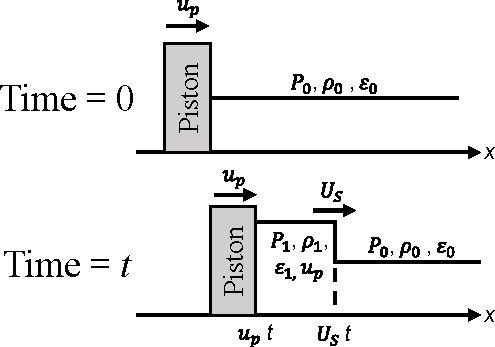
\includegraphics[width=0.6\textwidth]{figures/Theory/Piston.pdf}% Here is how to import EPS art
\caption{\label{fig:Piston} A piston moving at velocity $u_p$ drives a shock through a medium. The shock moves at velocity $U_S$, leaving material behind it in a new shock state denoted by the subscript 1. Based on a diagram in \cite{Zeldovich1966}.}
\end{figure}

Consider a material that is initially at rest, before being compressed by a Piston moving at a velocity $u_p$. This scenario is displayed in Figure \ref{fig:Piston}. After a time $t$ the piston itself has moved by a distance $u_pt$, while the disturbance (shock) it has generated has propagated with a `shock velocity' $U_S$ through the material to a position $U_S t$. Behind the shock the material is at the piston pressure and velocity $P$ and $u_p$, and at a new higher density $\rho_1$. Ahead of the disturbance, the material is unaffected. As the newly shocked material moves at velocity $u_p$, this quantity is known as the `particle velocity'.

Three equations can be derived based on the conservation of mass, momentum, and energy across the disturbance. Considering that the mass behind the shock front cannot have changed, the expression
\begin{equation} \rho_0 U_S = \rho_1 (U_S - u_p) \end{equation}
is obtained\footnote{Here, as in the following equations, $t$ and the area $A$ cancel from both sides of the equation during the derivation}. Considering the momentum of the material (which changes according to the impulse, arising from the difference in pressure either side of the boundary), leads to the equation 
\begin{equation} \rho_0 U_S u_p = P_1 - P_0. \end{equation}
Finally, considering the change in total energy (both internal energy $\epsilon$ and kinetic energy), which must equal the work applied by the piston as it moves the distance $ut$, results in the third equation 
\begin{equation} \rho_0 U_S (\epsilon_1 - \epsilon_0 + \frac{u_p^2}{2}) = P_1 u_p. \end{equation}

These equations relate the four shock variables $U_S$,$u_p$,$P$ and $\epsilon$ to one another. If the state of the material ahead of the shock is known, then finding any two of these variables allows the other to be calculated. They are referred to collectively as the Rankine-Hugoniot relations. They were derived here in a stationary frame (where the shock moves with velocity $U_S$), and are typically expressed as
\begin{equation} \rho_1 = \frac{\rho_0 U_S}{U_S - u_p}, \label{eqn: RH1 stationary} \end{equation}
\begin{equation} P_1 - P_0 = \rho_0 U_S u_p, \label{eqn: RH2 stationary} \end{equation}
\begin{equation} \epsilon_1 - \epsilon_0 = \frac{P_1 u_p}{\rho_0 U_S} - \frac{{u_p}^2}{2}. \label{eqn: RH3 stationary} \end{equation}

\subsection{Rankine-Hugoniot relations in a moving frame}

\begin{figure}
\centering
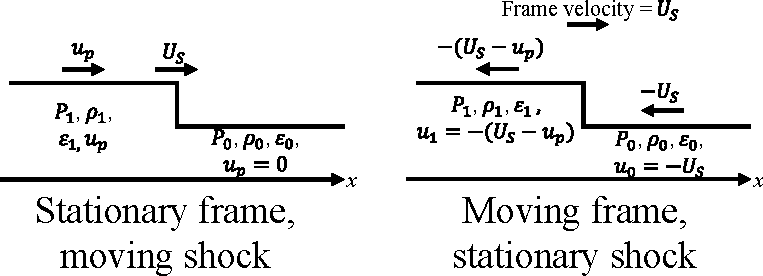
\includegraphics[width=0.8\textwidth]{figures/Theory/ReferenceFrames.pdf}% Here is how to import EPS art
\caption{\label{fig:ReferenceFrames} The shock as viewed in the two frames. In the stationary frame, the shock moves with velocity $U_S$, the shocked material with velocity $u_p$, and the unshocked material is stationary. In the moving frame, the shock is stationary, the shocked material has velocity $u_1$, and the unshocked material has velocity $u_0$. The other variables are unchanged.}
\end{figure}

Alternatively, the same equations can be considered in a moving frame, where the shock is stationary. The frame now moves at velocity $U_S$, as displayed in Figure \ref{fig:ReferenceFrames}. This means the unshocked material moves into the stationary shock front at a velocity $u_0 = -U_S$, while the material behind the shock moves away at the slower velocity $U_1 = -(U_S - u_p)$. This transformation can be applied to each of Equations \ref{eqn: RH1 stationary}, \ref{eqn: RH2 stationary} and \ref{eqn: RH3 stationary} to give the Rankine-Hugoniot relations in an alternative form,
\begin{equation} \rho_1 u_1 = \rho_0 u_0, \label{eqn: RH1 moving} \end{equation}
\begin{equation} P_1 + \rho_1 u_1^2 = P_0 + \rho_0 u_0^2, \label{eqn: RH2 moving} \end{equation}
\begin{equation} \epsilon_1 + \frac{P_1}{\rho_1} + \frac{u_1^2}{2} = \epsilon_0 + \frac{P_0}{\rho_0} + \frac{u_0^2}{2}. \label{eqn: RH3 moving} \end{equation}
These three relations can also be derived by integrating over the differential equations describing the conservation equations given in Section \ref{FluidDerivation}).

These equations can be further manipulated to derive some other useful expressions. Equations \ref{eqn: RH1 moving} and \ref{eqn: RH2 moving} can be used to find new expressions for the velocities $u_1$ and $u_0$, 
\begin{equation} u_1^2 = \nu_1^2 \frac{P_1 - P_0}{\nu_0 - \nu_1}, \label{eqn: RH moving u1} \end{equation}
\begin{equation} u_0^2 = \nu_0^2 \frac{P_1 - P_0}{\nu_0 - \nu_1}, \label{eqn: RH moving u0} \end{equation}
where $\nu$ is the specific volume, $\nu = \frac{1}{\rho}$. Substituting Equations \ref{eqn: RH moving u1} and \ref{eqn: RH moving u0} into Equation \ref{eqn: RH3 moving} then gives
\begin{equation} \epsilon_1 - \epsilon_0 = \frac{1}{2}(P_0 + P_1)(\nu_0 - \nu_1).\label{eqn: Hugoniot relation} \end{equation}

Equation \ref{eqn: Hugoniot relation} is known as the Hugoniot relation. The Hugoniot curve can also be defined, 
\begin{equation} P_1 = H(P_0, \nu_0, \nu_1), \end{equation}
which has a form which depends on that of the specific energy function $\epsilon(P, \nu)$. The form of the Hugoniot curve is notable as it is a function of two parameters - the initial state of the material $(P_0, \nu_0)$. The significance of this will be discussed in the next section.

\subsection{The Hugoniot} \label{The Hugoniot theory}

The Hugoniot curve describes the locus of possible shock states that can be achieved when a single shock is driven through a target with the specified initial state. It is formally defined as a function of $P$ and $\nu$ but the Rankine-Hugoniot relations mean it can be equivalently expressed as a function of any two of the shock variables, and it is often more convenient to discuss it in $(\rho, P)$ or $(u_p, P)$ space. Further discussion of this topic can be found in \cite{Forbes2012}.

\begin{figure}
\centering
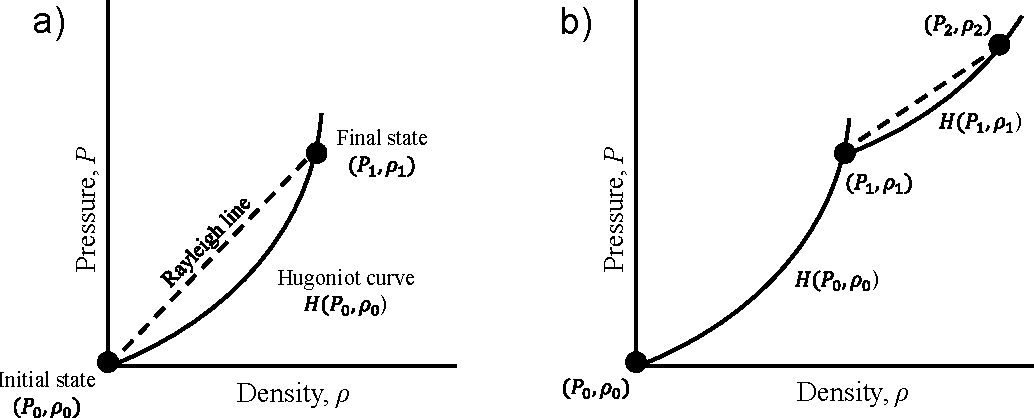
\includegraphics[width=0.8\textwidth]{figures/Theory/SecondaryHugoniot.pdf}% Here is how to import EPS art
\caption{\label{fig:SecondaryHugoniot} a) The principal Hugoniot in $(u_p, P)$ space. A shock compresses material in the initial state along a compression path described by the Rayleigh line to a shock state on the Hugoniot curve. The curve represents the range of possible shock states that could be achieved for a given initial state. b) If a subsequent shock passes through the material, the shock state it will generate lies somewhere on a secondary Hugoniot, which is a unique curve generated for the new initial condition (the shock state achieved by the first shock).}
\end{figure}

The dependence of the Hugoniot on the initial state is significant, as is highlighted in Figure \ref{fig:SecondaryHugoniot}. For the initial state $(u_0, P_0)$, the Hugoniot curve is plotted; this describes the states accessible by a shock from that initial point. Driving a shock with pressure $P_1$ through the target allows the shock state $(u_1, P_1)$ to be achieved. However, following this with a higher shock does not allow a new state on this curve to be accessed, due to the fact that the material ahead of this new shock is no longer in state $(u_0, P_0)$, is but instead $(u_1, P_1)$. To find the state achieved by this second shock requires a new Hugoniot curve to be plotted, $P_2 = H(P_1, \nu_1)$; this curve will pass through the state $(u_1, P_1)$, and describe the locus of states that the new shock can reach.

The Hugoniot curve describing the states that can be accessed from an initially unshocked material, $P_1 = H(P_0 = 0, \nu=\nu_0)$, is particularly significant for two obvious reasons; most materials begin experiments unshocked (and so the first shock state achieved will be on this curve), and the states on this curve are the easiest to measure and access. This curve is known as the `principal Hugoniot'. This curve can be populated experimentally by measuring the state achieved when shocks of different strengths are passed through initially unshocked material.

It is also worth noting that the Hugoniot curve is not the path that the material takes through $(P, \nu)$ space as it is compressed (rather, it is the possible end states of such a compression). The compression path is given by a different curve called the `Rayleigh line' \cite{Forbes2012}. The Rayleigh line is described by Equation \ref{eqn: RH2 stationary}, repeated below:
\begin{equation} P_1 - P_0 = \rho_0 U_S u_p.  \end{equation}
Note that in $(u_p, P)$ space, the Rayleigh line is a straight line with a gradient of $Z = \rho_0 U_S$. If a shock travels through the material with a shock velocity $U_S$, then the final shock state will be the intercept between the Rayleigh line and the Hugoniot. This gradient $Z$ is called the shock impedance, and is significant when considering shocks between different materials. It's also important to note that using Equation \ref{eqn: RH2 stationary} requires all velocities to be in the stationary frame, where the material ahead of the shock is stationary\footnote{In the case shown in Figure \ref{fig:SecondaryHugoniot} (b) where this material ahead of the shock has been preshocked, the `stationary frame' is now moving so that the material ahead of the shock appears stationary. If the material has been preshocked to a pressure $P_a$ and velocity $u_a$, and the new shock moving at $U_S$ drives the material to a pressure $P_b$ and velocity $v_b$, then the Rayleigh line would be given by $P_b - P_a = \rho_0 (U_S - u_a) (u_b - u_a).$ }.

\subsection{Material interfaces and impedance matching \label{IMTheory}}

The previous sections have considered shocks moving through a single material; in this section, the interface between materials will be considered following the descriptions given in \cite{Forbes2012} and \cite{Davison2008}. Imagine a shock $S_1$ travelling through material A, which then reaches an interface with material B. Some fraction of the shock energy will be transmitted across the interface into material B, while some will be reflected into material A. The pressure behind the reflected shock $P_R$ is given \cite{Colvin2013} by 
\begin{equation} \frac{P_R}{P_1} = \frac{Z_2 - Z_1}{Z_2 + Z_1}.  \end{equation}
Three illustrative cases are useful to consider. If the impedances of the two materials are very similar $Z_2 \approx Z_1$, the reflected shock pressure will be effectively zero and almost all the shock energy propagates into the new material. If there is a high impedance mismatch between the materials, then a large fraction of the shock energy is reflected. If the new material is higher impedance $Z_2 > Z_1$, then the reflected pressure is positive and a shock is reflected. If the new material is instead low impedance $Z_2 < Z_1$ then a rarefaction/relaxation wave is instead reflected.

The state achieved either side of the interface after the shock crosses it can be found through an impedance matching calculation. This relies on a key principle. After the shock has crossed the interface, the material on either side is in the state achieved by the transmitted/reflected waves $S_2$ and $S_3$. For the two materials to remain in contact, it is required that the pressure $P$ and particle velocity $u_p$ of the material either side of the boundary must be equal - if this were not the case, the boundary would not be in equilibrium, or the two layers would separate. This enables impedance matching calculations, where the state in each material following the shock crossing the interface can be determined.

\begin{figure}
\centering     %%% not \center
\subfigure{a)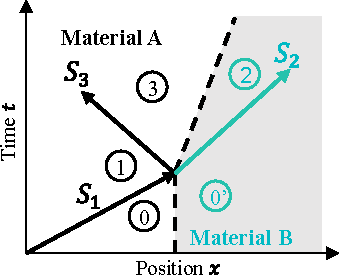
\includegraphics[width=.45\textwidth]{figures/Theory/ShockDiagram.pdf}}
\subfigure{b)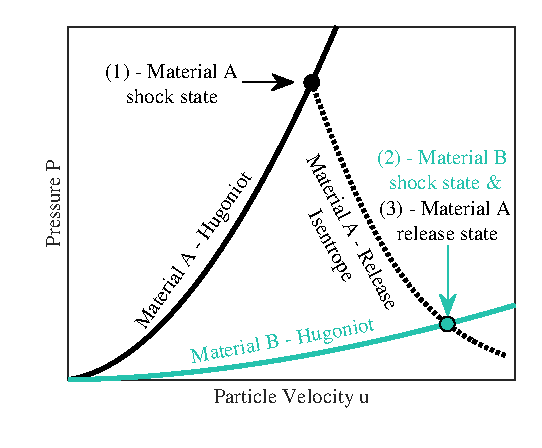
\includegraphics[width=.45\textwidth]{figures/Theory/MatlabIM1.eps}}
\caption{ \label{fig:ShockDiagramAndIMTheory1} a) x-t diagram showing a shock transiting across the interface from a high impedance material into a low one. The dashed line shows the material interface, while the arrows show the shocks. The shock/rarefaction waves are refered to as $S_n$, while the shock states are refered to by the numbers. b) $(u, P)$ plot showing the impedance matching graphically. $S_1$ shocks material in state (0) to a state (1) on the Hugoniot for material A. Rarefaction wave $S_3$ causes A to relax from (1) to a state (3) on the release isentrope for A. Shock $S_2$ shocks B from state (0') to state (2) on the Hugoniot of B. The impedance matching criteria means that (2) and (3) are equivalent in $(u, P)$ space, and thus this state is the intercept of these two curves.}
\end{figure}

This is shown graphically for the case where the second material is lower impedance in Figure \ref{fig:ShockDiagramAndIMTheory1}. Two materials, A and B, are in contact with an interface between them. They are both initially unshocked, in states described as (0) and (0') respectively. The pressure and particle velocity of state (0) can be described as $(u_0, P_0)$ - as both (0) and (0') are unshocked and stationary, both $P$ and $u$ are in fact 0. Note here that the velocity $u_n$ is this section is just used to refer to the velocity of the state labelled $n$, rather than suggesting that a particular reference frame is being used - in fact, it is simplest to do the calculation in the stationary frame.

An initial shock $S_1$ travels through material A shocking it to the state (1) with $(u_1, P_1)$, which must by definition lie on the principal Hugoniot for material A. $S_1$ reaches the interface between the two materials, and this generates a rarefaction wave $S_3$ which travels back into material A, and a shock wave $S_2$ which propagates through material B. As material B is unshocked, the new state $(u_2, P_2)$ lies on the principal Hugoniot for material B. Rarefaction wave $S_3$ travels through the pre-shocked state $(u_1, P_1)$, and causes it to relax to a new state $(u_3, P_3)$. This relaxation occurs along another curve known as the release isentrope, which describes the locus of states that the material could relax to given it's shocked initial state of $(u_1, P_1)$. 

It is clear from Figure \ref{fig:ShockDiagramAndIMTheory1} (a) that after the shock has crossed into material B, the states either side of the interface are the shocked material B in state (2) and which lies on the B Hugoniot, and the relaxed material A in state (1) which lies on the A release isentrope. The impedance matching criteria requires that both pressure and particle velocity must be constant across the interface, and as such $P_3 = P_2$ and $u_3 = u_2$. This condition is satisfied at the intercept of these two curves in $(u, P)$ space, as shown in Figure \ref{fig:ShockDiagramAndIMTheory1} (b). Therefore, the intercept of these two curves\footnote{There are two things to note here. 1) There is only one state which satisfies this condition. However, if the shock $S_1$ strength is changed, the state $(u_1, P_1)$ is changed, and thus the release isentrope (which depends on this initial state) also changes - meaning that the impedance matching criteria where the Hugoniot B and release isentrope are satisfied now also occurs at a different point. 2) While the $(u, P)$ state of the two materials is equivalent, the Rankine-Hugoniot equations used to calculate the other variables reference the initial state of the material being considered - meaning that the other shock variables for these materials will not be equal.} defines both states (2) and (3). 

The general principle is the same if B has a higher impedance than A, but with a few changes. Here, the wave $S_2$ is now a shock wave rather than a rarefaction wave. This means that the state (3) is no longer a relaxed state on the release isentrope, but a new shock state which lies somewhere on a secondary Hugoniot of A (i.e. a Hugoniot generated for the initial conditions of state (1)). This also results in a pressure $P_3 = P_2$ which is greater than $P_1$. However, the impedance matching condition $P_3 = P_2$ and $u_3 = u_2$ still applies, and thus in this case the states (2) and (3) are instead the intercept between the principle Hugoniot of material B with this new secondary Hugoniot of material A (replacing the release isentrope).

\subsection{Measuring shock states experimentally \label{IMTheoryMeasurements}}

%It was shown earlier in this section that the Rankine-Hugoniot relations allow all the shock variables associated with a shock state to be calculated, if at least two of the variables (and the state of the unshocked material) are already known. Experiments to measure shock states therefore require the measurement of any two of these variables. `Absolute' shock state measurements measure two such variables directly. 

%However, impedance matching provides a way to determine the shock state of a material by only measuring one of these variables directly. This relies on the situation described in the previous subsection. A known reference material, which is already well-characterised, is placed in contact with the material of study. Aluminium or quartz are typical examples. A shock is then driven through the reference material, such that it crosses the interface into the material being studied. As discussed, this will result in a shock/rarefaction (depending on the relative impedance) wave propagating back into the reference, and the pressure and particle velocity in the reshocked/relaxed reference and the shocked material of study will be equal.

%This is performed in such a way that the shock velocity can be measured in both materials. The shock velocity in the reference material during the first shock is measured, and this is used to plot the Rayleigh line $P_1 = \rho_0 D u$ in the reference. The intercept of the Rayleigh line and the Hugoniot defines the shock state that the reference material reaches after the first shot. When the reflected shock/rarefaction wave propagates back through the reference, this material will be shocked/relaxed according to an as yet undetermined point somewhere on the known reference Hugoniot/release isentrope. 

%Following the theory in the previous section, it is clear the 

It was shown earlier in this section that the Rankine-Hugoniot relations allow all the shock variables associated with a shock state to be calculated, if at least two of the variables (and the state of the unshocked material) are already known. `Absolute' shock experiments aim to measure two such variables directly. However, impedance matching experiments make use of the impedance matching criteria to enable the shock state in a material to be determined by measuring only one variable (typically the shock velocity) in two different materials: the material of study, and a reference material. This is often simpler experimentally.

\begin{figure}
\centering
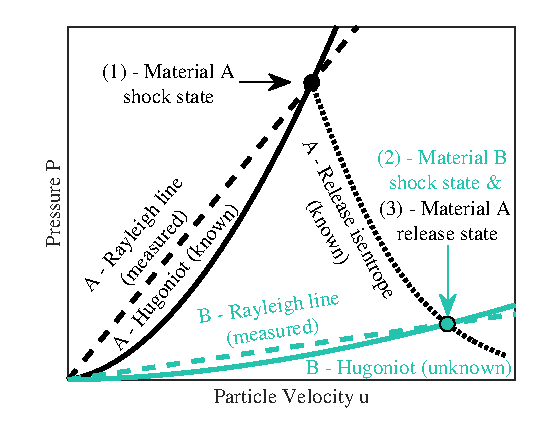
\includegraphics[width=0.6\textwidth]{figures/Theory/MatlabIM2.eps}% Here is how to import EPS art
\caption{\label{fig:IMTheory2} A $(u, P)$ plot as in Figure \ref{fig:ShockDiagramAndIMTheory1}, showing how impedance matching is used experimentally. Material A is a reference, where the Hugoniot (solid black line) and release isentrope (dotted black line) are known. Measuring the shock velocity of $S_1$ in A allows the Rayleigh line to be plotted (dashed black line) - the intercept of this with the known Hugoniot for A allows state (1) to be determined. Measuring the shock velocity of $S_2$ in B also allows a Rayleigh line to be plotted for this shock (dashed teal line). The intercept of this line with the known release isentrope A allows the state (2), a shock state of B which lies on the unknown Hugoniot of B (solid teal line), to be calculated.}
\end{figure}

Consider the situation described in the previous section, but with material A now being a known reference (which means that the relevant curves, such as the Hugoniots and the release isentrope, are already known) and material B being the material of study. Imagine that an experiment is conducted so that the shock velocity of $S_1$ in material A and of $S_2$ in material B are measured.

Measuring the shock velocity $U_{S_1}$ allows the Rayleigh line for this shock to be plotted. As discussed in Section \ref{The Hugoniot theory}, the achieved shock state in material A will be the intercept of the Rayleigh line and the material Hugoniot. As A is a reference material where the Hugoniot is measured, this intercept can therefore be identified, and the shock state (1) determined. This is shown in Figure \ref{fig:IMTheory2}. This shock state (1) can then be used to calculate the release isentrope\footnote{This example is given again for where B is lower impedance than A. If B is higher impedance, replace all mentions of the isentrope with the secondary Hugoniot, and any mention of `relaxed' material A to `reshocked' material A.} for material A. Again, as A is a reference, this isentrope is already known.

Measuring the shock velocity $U_{S_2}$ enables the Rayleigh line for the shock in material B $S_2$ to be plotted, and the intercept with the Hugoniot for material B would define the shock state for that material. As material B is the material for which the shock behaviour is being investigated, this Hugoniot is not known. Howver, the impedance matching criteria means that this is the same $(u, P)$ state achieved in the relaxed (or reshocked) material A, and thus also lies on the release isentrope for this material. The shock state (2) of material B can therefore be identified from the intercept of the release isentrope for A and the Rayleigh line for B. This shock state is thus determined through only measurements of the two shock velocities, and knowledge of the reference material.


%\begin{savequote}[8cm]
%\textlatin{Neque porro quisquam est qui dolorem ipsum quia dolor sit amet, consectetur, adipisci velit...}

%There is no one who loves pain itself, who seeks after it and wants to have it, simply because it is pain...
% \qauthor{--- Cicero's \textit{de Finibus Bonorum et Malorum}}
%\end{savequote}

\chapter{Definitions of key terms} \label{ch:definitions}

\minitoc

\section{Introduction}

Many of the key terms that are ubiquitous in ICF, such as `hotspot' and `ignition', have no single agreed upon definition. This can make it difficult to compare results between different published works, and can mean the use of such terms is ambiguous. This chapter will discuss the definitions for a range of terms and quantities that will be used throughout this thesis, along with the details of exactly how these quantities were evaluated for the simulations presented in later chapters.


\section{Convergence ratio}
The definition of convergence ratio used in this work is 
\begin{equation} \mathrm{CR} =  R_\mathrm{I}/R_\mathrm{HS}, \label{CR} \end{equation} 
where $R_\mathrm{I}$ is the initial interior radius of the DT layer, and $R_\mathrm{HS}$ is the radius of the hotspot. This is the same definition as used in the works by Olson \textit{et al.} \cite{Olson2016} and Zylstra \textit{et al.} \cite{Zylstra2018}, and was selected to ensure compatibility with their findings. This parameter can also be referred to as the `hot-spot convergence ratio', and remains a common definition of convergence ratio for wetted-foam research \cite{Olson2021}.

Other definitions for convergence ratio also exist. Some papers define the initial radius $R_\mathrm{I}$ as the `initial inner radius of the shell' \cite{Craxton2015} or the `initial radius of the DT layer' \cite{Haines2017a}; these are likely the same definition as discussed previously, but the phrasing is potentially ambiguous and could also apply to the DT/ablator interface. Alternatively, a `capsule convergence ratio' is also used where the radius $R_\mathrm{I}$ is instead defined as the outer radius of the capsule, including the CH ablator \cite{Lindl2004}. Further ambiguity is inserted through the $R_\mathrm{HS}$ term. This is often stated as simply the hotspot radius \cite{Olson2016, Olson2021}, but can also be described as the `minimum' hotspot radius, the hotspot radius at peak compression \cite{Craxton2015}, or the stagnated outer radius of the hotspot \cite{Zylstra2018}. These terms are all interpreted to mean the minimum achieved hotspot radius, but it is noted that this does not necessarily occur at the the time of stagnation (itself a poorly defined term) or peak compression. More significant is the ambiguity in how the hostpot radius is identified, as discussed in the following section.

The convergence ratio is often evaluated in simulations where alpha deposition has been turned off \cite{Craxton2015}. This is because alpha deposition leads to increased hotspot pressure, which in turn will decrease the convergence ratio of the capsule. However, if the experimental performance does not match that of the simulations, then this pressure will be reduced and the capsule may converge further before burn begins; and thus using the value derived without alpha deposition represents a worst-case scenario. In this thesis, convergence ratio was calculated with alpha-heating included. This was done for convenience during the capsule optimisation in Chapter \ref{ch-lowCR}, since otherwise two simulations would have been required for each set of parameters (one with alpha-heating to enable calculation of the gain, and one without to enable calculation of the convergence ratio). The focus of this work was largely on achieving break-even, and at these gains the discrepancy between burn and no-burn parameters is minimal (this effect only starts to become significant for gains of around 10 and above \cite{GoncharovPersonalComm}).

\section{Hotspot and shell}

\begin{figure}[ht]
	\centering
	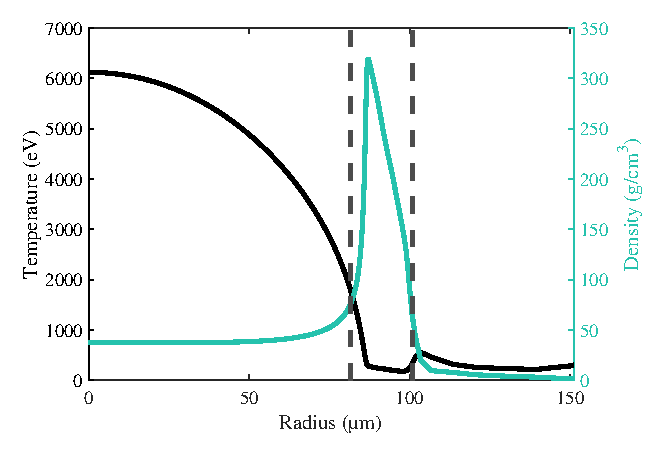
\includegraphics{figures/LowCR/HSDefn.eps}
	\caption{Ion temperature (black) and density (teal) at the time of maximum compression, for an implosion simulated in \texttt{HYADES}. The two dashed lines indicate the position of the hospot and shell radii using the definitions defined in the text.}
	\label{fig:HsDefn}
\end{figure}

The term `hotspot' is used to refer to the low-density, high temperature region at the centre of the ICF capsule, while the `shell' is the cooler high-density region surrounding it. A plot of a capsule at peak compression, such as that shown in Figure \ref{fig:HsDefn}, clearly shows the relevance of this description. However, where the exact interface between the two lies is not clearly defined. This is particularly true if one wishes to extend the concept of the shell to earlier stages in the implosion before stagnation (for instance, in order to calculate the implosion velocity). There is no accepted definition for this interface, and the definition used in a particular paper is not usually provided; the only definition found was in \cite{Olson2021}, which defined the hotspot as the central region where the temperature was above 5keV. This is not a useful definition for small non-igniting capsules, which despite showing similar temperature and density behaviour to Figure \ref{fig:HsDefn} may not achieve such temperatures anywhere in the capsule. This definition would also poorly describe the capsule in Figure \ref{fig:HsDefn}, where quite a large region of low density material would be considered part of the shell. The definition of these parameters is particularly important, since many other terms (including the convergence ratio) are defined with reference to them.

As such, a new definition for hotspot/shell was identified for this work. The hotspot/shell interface (or `hotspot radius') is defined as the radius at which the density has increased by $1/e^2$ of the difference between the central hotspot density and the peak density in the shell. The shell outer radius is defined as the radius where the density has decreased to $1/e^2$ of the peak value. In Figure \ref{fig:HsDefn} this places the two boundaries at the dashed lines, which matches well with the qualitative description. As this definition is based on density, it works throughout the early stages of the implosion - defining a 'shell' which could be used for the calculation of other quantities. 

\section{Hotspot / shell temperature}
The hotspot and shell temperatures referred to in this thesis are the mass-averaged ion temperatures over the hotspot and shell zones respectively. This (along with the definition for convergence ratio) is a clear example of how defining the hotspot and shell influences other important parameters.

\section{Areal density}

Despite areal density typically being referred to as $\rho R$, which suggests that it is the product of the density and the radius at a given position, the more accepted and commonly used version \cite{Craxton2005, Betti2005, Abu-Shawareb2022} of this quantity is \begin{equation} \rho R = \int_{R_1}^{R_2} \rho \cdot dR, \end{equation} the integral of the density $\rho$ with respect to radius $R$ over the region being considered\footnote{My first paper on this work defined $\rho R$ simply as the mass averaged product of these two quantities, which was replaced with the integral form for subsequent papers.}. Definitions for areal density are often not provided, and some works do indeed discuss $\rho R$ as the product of these two quantities \cite{Atzeni2008}.

In this thesis, $\rho R$ is used to refer to the integral version of this quantity. The major benefit of this definition is that the areal density of different regions sums linearly. This means that the total capsule areal density is the sum of the hotspot areal density and the shell areal density, which makes intuitive sense. Areal density can thus be thought of as a measure of how much DT fuel an alpha particle must move through, when generated at the centre of the capsule and travelling (in a straight line) outwards - which highlights why this quantity is important for alpha absorption, self-heating, and thus gain. It also correlates well to the experimentally determined `neutron averaged' areal density, which is an average of the areal density across the neutron line of travel between the point of generation and the detector.


\section{In-flight aspect ratio}

The definition for the in-flight aspect ratio of the capsule used in this work is \begin{equation} \mathrm{IFAR} = \frac{R_\mathrm{shell}}{t_\mathrm{shell}}, \end{equation}
where $R_\mathrm{shell}$ and $t_\mathrm{shell}$ are the shell radius and thickness. This quantity is evaluated when the capsule has been compressed to two-thirds of it's initial radius, in accordance with the common definition provided in the review article by Craxton \textit{et al.} \cite{Craxton2015} (other works evaluate the IFAR at different times, such as when the shell has converged by a factor of one third \cite{Radha2011}). In the analysis performed in these simulations, the IFAR is evaluated at the point when the shell outer radius (as defined previously) reaches 2/3 of the initial inner radius of the wetted-foam layer. The shell thickness is defined as the shell radius minus the hotspot radius. It should be noted that some works define the shell radius as the position of peak shell density - the definition for $R_\mathrm{shell}$ used in this thesis is larger, and will result in a slightly larger IFAR value than using this alternative definition.

\section{Implosion velocity}

The term `implosion velocity' is typically used to refer to the peak velocity achieved as the capsule implodes. The implosion velocity used in this work was a volume averaged velocity across the material used in the shell. This should more correctly be a mass-averaged implosion velocity, but the difference in these quantities is marginal. 

\section{Laser intensity}

The laser intensity will form an important part in the definition in Chapter \ref{ch-lowCR} for the low-instability regime. However, laser intensity is a function of the area over which the laser acts; if the same power is absorbed over a smaller surface area (i.e. as the capsule radius decreases) the intensity will increase.

In this thesis, the intensity compared to the low-instability criteria is calculated using the initial capsule radius. This was done for convenience; since the initial radius of the capsule is known in advance, the laser power can thus be chosen in order to ensure an appropriate intensity (when using this definition). However, it is also reasonable to assume that the time-dependent intensity at the critical density will not increase much beyond this value, as while the radius decreases the coronal plasma would be expected to decrease the power of the incoming laser through absorption and scattering processes.

\section{Yield, gain and bang time}

Yield (or `fusion yield') throughout this thesis is used to refer to the neutron yield, or the energy carried by the neutrons that will escape the fuel assembly and could thus potentially be captured. \texttt{HYADES} outputs a `total yield' which includes the energy of the alpha particles, and the neutron yield is 80 \% of this value. The number of fusion-generated neutrons can be obtained by dividing the neutron yield by the 14.1 MeV neutron energy \cite{Atzeni2008}.

The term `gain' is used throughout this thesis to refer to the `total' or `target' gain, which is defined as \begin{equation} G = \frac{Y_{tot}}{E_{las}}, \end{equation} where $Y_{tot}$ is the neutron yield and $E_{las}$ is the input laser energy. Alternative variants on gain include capsule gain ($G_{cap} = Y_{tot / }E_{abs}$, which compares the yield to only the energy absorbed by the capsule $E_{abs}$) and fuel gain ($G_{fuel} = Y_{tot} / E_{fuel}$, which compares yield instead to the energy absorbed by the DT fuel $E_{fuel}$), both of which are significantly larger \cite{Atzeni2008, Abu-Shawareb2022}.

The bang time of the implosion is defined as the time of maximum neutron generation (i.e. where the peak number of fusion reactions occur) \cite{Craxton2015}.

\section{Adiabat}

The adiabat (or isentrope parameter) of an ICF capsule is used as a measure of the entropy of the cold, highly compressed DT fuel. This is done through comparison with a cold gas with Fermi-degenerate electrons. It is defined as \begin{equation} \alpha = \frac{P(\rho, T)}{P_{deg}(\rho)}, \label{eqn:adiabat} \end{equation} where $P(\rho, T)$ is the pressure of the DT fuel for which the adiabat is calculated, while $P_{deg}(\rho)$ is the pressure for the Fermi-degenerate DT at the equivalent density. This can be calculated using \begin{equation} P_{deg}(\rho) = A_{deg} \rho^{5/3}, \end{equation} where $\rho$ is the density in \unit{\gram\per\centi\meter\cubed}, and $A_{deg} = $ \num{2.17e12} \unit{(\mathrm{erg}/\mathrm{g})/(\mathrm{g}/\mathrm{cm}^3)^{2/3}} for equimolar DT \cite{Atzeni2008}. 

There are multiple ways such a definition can be evaluated, and this is discussed in \cite{Haan2011}. The adiabat is most commonly quoted at the time of peak implosion velocity \cite{Park2014}, but it can also be evaluated post-stagnation. The quoted adiabat value can be either a mass-weighted average, or the minimum adiabat in the DT fuel at that time. If it is an average, the range over which the average is taken can also influence the results. 

An alternative way of calculating adiabat is also provided in \cite{Haan2011}. Here, they instead calculate a mass-averaged entropy at the peak implosion velocity. The equation of state for the DT is then used to calculate the pressure for DT at 1000 \unit{\gram\per\centi\meter\cubed}, on the isentrope defined by that particular entropy value. This calculated pressure is referred to as $P_{cold}$, and replaces the Fermi-degenerate pressure ${P_{deg}(\rho)}$ in the previous equation for adiabat. This is because the cold DT fuel at typical densities achieved in the shell at peak implosion velocity may not be fully ionised, and thus $P_{cold}$ may be lower than ${P_{deg}(\rho)}$. The pressure definition of adiabat does not well account for the density dependence of the DT entropy, and can give behaviour that is non-monotonic in entropy \cite{HainesPersonalComm}. Another alternative definition is to again calculate the mass-averaged entropy of the DT fuel, and then use this value in a fitting formula to calculate the adiabat directly \cite{Haan2011, Haines2022}.

Adiabat does not play a significant role in this thesis, and adiabat values are not reported. In part, this was due to difficulties in this calculation; the adiabat value calculated from Equation \ref{eqn:adiabat} was found to be dependent upon the selection of zones used. \texttt{HYADES} does not return the entropy of the fuel, which means that the alternative definitions could not be used.

%In this work, the reported adiabat is the mass-averaged adiabat of DT in the capsule shell. The minimum adiabat is also calculated, which is the minimum adiabat across the DT zones in the shell. Both of these quantities are calculated as a function of time, and increase as the implosion progresses.

\section{Ignition and break-even}
Of all the ICF parameters, `ignition' is probably the most ambiguous. The National Research Council in 1977 defined ignition as the point at which the fusion energy produced exceeded the laser input \cite{NRC}; this is easy to understand and describes an important milestone in fusion research, but is not linked to any major physics transition/threshold within the capsule. There are both alternative definitions (for example, it can be defined as the point at which a burn wave starts to propagate through the cold shell \cite{Christopherson2020}), and multiple ways that such definitions can be quantified. When the NIF shot N210808 achieved a yield of 1.3 MJ, this ambiguity meant that it had to be evaluated against nine different criteria in order to claim `ignition' had been achieved \cite{Abu-Shawareb2022}. It was able to satisfy these criteria with high confidence despite not achieving the NIC criteria (which was finally satisfied by the December 2012 shot).

Due to this ambiguity and lack of single clear definition, the term `ignition' has been avoided where possible in this thesis. Where it is used, it is done so causally and simply means to achieve a well-performing capsule with high-gain. The term `break-even' is used instead, which has an agreed upon definition of a gain of unity (meaning that it is the same as the NIC ignition criteria, but without the ambiguity).
%\begin{savequote}[8cm]
%Alles Gescheite ist schon gedacht worden.\\
%Man muss nur versuchen, es noch einmal zu denken.

%All intelligent thoughts have already been thought;\\
%what is necessary is only to try to think them again.
 % \qauthor{--- Johann Wolfgang von Goethe \cite{von_goethe_wilhelm_1829}}
%\end{savequote}

\chapter{Low convergence ratio implosions} \label{ch-lowCR}

\minitoc

\section{Introduction}

Wetted-foam ICF capsules, consisting of a low-density foam saturated with liquid DT, can be used in place of conventional DT ice capsules. The use of liquid (rather than frozen) DT means that such capsules are fielded at a higher initial temperature, between 20 and 26K. This higher temperature leads to a higher density of DT vapour within the central void of the capsule, ranging between 0.6 and 4.0 \unit{\milli\gram\per\centi\meter\cubed} \cite{Olson2016}. Higher vapour densities lead to less capsule convergence, and thus varying the temperature of wetted-foam capsules provides an excellent opportunity to explore how implosion physics varies with convergence.

In ideal (1D) implosions, increasing the convergence ratio of the capsule leads to higher areal densities, and higher fusion yields. However, it has also been demonstrated that lower convergence implosions are less susceptible to hydrodynamic instability growth, and initial experiments at the National Ignition Facility using low convergence-ratio implosions of wetted foam capsules demonstrated good agreement with simulations  \cite{Olson2016, Zylstra2018}. The experimental fusion yield of a capsule is a balance of two effects: the increase in ideal fusion yield as the convergence ratio increases, and the decrease in agreement between experiment and simulation.

In this chapter, the possible fusion yield of low-convergence ratio implosions of wetted-foam capsules is explored in a large-scale simulation campaign. A regime was identified (based on low-convergence ratio, and other implosion criteria) where instability growth is expected to be low, and one-dimensional simulations would provide a reasonable estimate of expected performance. This was intended as a first exploration of what may be possible in such a regime; if sufficiently high fusion performance could be obtained, it may be the case that this coupled with the higher-than-typical agreement between simulation and experiment in this regime may in fact outperform higher convergence implosions in experiments.

In Section \ref{sec: PreviousLowCRResults}, the results of previous experiments and simulation efforts relevant to low-convergence implosions are discussed. In Section \ref{sec: Low-Instability} a range of different parameters influencing instability growth is considered - culminating in four criteria to minimise instability growth used to define this new regime, and thus (hopefully) ensuring that 1D simulations are reasonably accurate. The capsule design and laser pulse sequence that will be used in the simulation campaign is then considered in Section \ref{sec: CapsuleAndPulse}. The actual simulation campaign is then discussed in Section \ref{sec: OptimisationCampaign}, before the results are presented in Section \ref{sec: LowCRResults}. Finally, the limitations of this approach are considered in Section \ref{sec: LowCRLimitations}, and ways that the work could be developed further are discussed.



%One of the promising possibilities that wetted foam capsules enable is a degree of control over the convergence ratio that is not possible with conventional capsules. Wetted-foam targets contain liquid DT wicked in a carbon foam. They are thus fielded at higher temperatures between 20 and 26 K (where DT is in liquid form), which in turn leads to higher vapour pressures ranging from 0.6 \unit{\milli\gram\per\centi\meter\cubed} to 4.0 \unit{\milli\gram\per\centi\meter\cubed}. These higher vapour pressures enable lower convergence ratios to be achieved. Not only this, but it also provides a way to control the convergence ratio largely independently from other implosion properties, by varying the temperature at which the capsule is fielded \footnote{Doing this has a small impact on some of the other properties, but this is essentially negligible.}. This enables the impact of convergence ratio on an ICF implosion to be explored.

%The first wetted foam target was shot on the NIF in 2016, in shot N160421. The results were interesting; neutron yield of \hl{VALUES} were achieved, which were promising and suggested a good level of performance could be achieved with these capsules. More promising however was the fact that agreement between the experimental and simulated results were high, suggesting a capsule that was performing roughly as expected, and without significant instability growth. Further shots presented by Zylstra \textit{et al.} confirmed this, and showed explicitly the link with convergence ratio. At low convergence ratio, the agreement with 2D simulations were very high, and as this increased the agreement rapidly began to get worse. 

%This raised the prospect of a new, alternative approach to ICF experiments. Previous approaches had targeted high convergence ratio implosions with very large gains, but failed to achieve them due to poor agreement with simulations - efforts were then ongoing to improve this agreement by reducing the instability growth. The alternative to this would be to operate at low-convergence ratio, in a regime where the agreement between simulation and experiment inherently appeared to be high. If performance could be explored in this regime in simulations and a high-performing design could be identified, then it could be reasonably expected that the experimental performance would also be high. The question was whether it would be possible to achieve sufficiently high performance at low convergence ratio to make such an approach worthwhile.

%The other benefit of this approach was that these low convergence ratio implosions were exhibiting low instability growth. This meant that the performance of such implosions could be reasonably well approximated as one-dimensional, allowing 1D simulations to be used to explore the performance. As 1D codes are relatively simple and quick to run (particularly compared to their 2D or 3D equivalents), this meant that a large-scale simulation campaign would be feasible.

%Such a campaign was therefore performed to explore the possible performance of wetted-foam capsules at low convergence ratio at a range of laser energies, and is described in this chapter. First, some of the previous results of low-convergence work is discussed, and the NIF shots are considered in further detail. Secondly, in an attempt to ensure instability growth is minimal and thus 1D simulations are accurate, other 1D implosion properties that correlate with instability growth are considered; a low-instability regime is thus identified which will set the boundaries for this campaign. Definitions of key parameters are then defined, describing the key metrics through which the simulated implosions will be judged.

S%ection then discussed the form of the implosions considered, in terms of the laser profile and the capsule design. The simulation code and paramters used to simulate these implosions are then discussed in SECTION, before SECTION discusses how the simulation campaign was actually performed and conducted. The results achieved in this campaign are then presented and discussed in SECTION, before a discussion of the limitations of this campaign and the efforts taken to model the impact of these. Finally, a discussion on benchmarking of the code is included.

\section{Wetted foam capsules and low convergence ratio} \label{sec: PreviousLowCRResults}

\subsection{Experimental results}

The first DT-wetted foam shot on the NIF (designated N160421) was performed in 2016, and was reported on by Olson \textit{et al.} \cite{Olson2016}. The results were interesting; a promising $(4.5 \pm 0.1) \times 10^{14}$ neutrons were generated, which suggested that a good level of performance could be achieved with such implosions. More impressive however was the close agreement between the simulation and experiment. 2D simulations were able to match a wide range of implosion metrics (including temperatures, bang time, hotspot radius and inferred pressures) to within the experimental error. These metrics were also very well described even by a 1D RAGE simulation (with a mix model included), which gave a ratio between experimental and simulated yield of nearly 80 \%. 

N160421, and subsequent wetted-foam shots N160626 and N161204, were then discussed by Zylstra \textit{et al.} \cite{Zylstra2018} in 2018. These three shots spanned a convergence ratio range of 12-20. This confirmed that convergence ratio could indeed be controlled using initial capsule temperature. These shots were then simulated using the HYDRA and xRAGE codes. The agreement was again very good at low convergence ratio (with yield and ion temperature agreeing to within 5 \% for N160421 with a convergence ratio of 12), but the discrepancy increased with convergence ratio resulting in a experimental yield for the CR=20 shot that was only 30 \% of that predicted by the simulation. The intermediate shot, with a convergence ratio between 16 and 17, showed a good agreement of above 70 \%\footnote{It should be noted that the exact reason for this discrepancy could not be identified in \cite{Zylstra2018}.}. These NIF shots therefore showed that wetted-foam capsules could be used to generate low-convergence ratio shots on the NIF, and that the agreement with simulations at low-convergence ratio was relatively high.

This was not the first time a link between low convergence-ratio and agreement with simulation was observed; the same result is highlighted in the following (non-exhaustive) collection of references \cite{Kato1996, Nishimura2000, Meyerhofer2001, Li2002, Lindl2004, LePape2014, Khan2016, Haines2017a}. This agreement was identified as far back as 1980 \cite{Key1980}, where it was observed that lower initial aspect ratios (thicker shells as a function of radius - resulting in lower implosion velocities and less convergence) resulted in performance that was more 1D-like; the low laser energies available at the time however made it unfeasible to pursue high gain in this regime. The other innovation provided by wetted-foams was the ability to vary convergence ratio (almost) independently from other parameters, by varying the initial temperature and thus vapour density of the capsule.

While the NIF shots discussed so far were indirect-drive, similar links between convergence ratio and 1D-like performance have also been observed in direct-drive shots on Omega. Regan \textit{et al.} observed that the hotspot pressure and compressed areal density of capsules using DT ice layers (rather than wetted-foams) reached 90 \% of the 1D simulated values for convergence ratios below 17 and adiabats greater than 3.5 \cite{Regan2016}. When the convergence ratio was increased past 17 a rapid drop-off occurred, which shows good qualitative agreement with the trend in yield observed on the NIF shots. This shows that this relationship applied for both indirect and direct-drive implosions, using both DT-ice or DT-wetted foam layers.


\subsection{Simulation work} 

This topic has also been explored through simulation work. 2D simulations were previously used to investigate how the yield of wetted foam capsules with varying vapour density (and thus convergence ratio) changed, for different amplitudes of a Legendre $P_4$ flux asymmetry. As expected, they found that the higher vapour density / lower convergence ratio implosions were significantly more robust to this instability, with a higher ratio of 2D to 1D yield \cite{Olson2013}. Simulations performed in preparation for the NIF shots suggested that sensitivity to capsule instability growth and x-ray flux assymmetries increased with convergence ratio, leading to strong agreement between 2D and 1D simulations for CR=15 shots when surface roughness was applied compared to much worse agreement for high convergence ratio shots - leading to a hypothesis that using low convergence ratios would lead to reduced instability growth and a robust predictive capability \cite{Olson2016a}. 

High resolution 2D xRAGE simulations performed in 2017 investigated full-scale wetted foam capsules with a variety of `asymmetry seeds'. These simulations showed when only surface roughness and drive asymmetries were included yield increased with convergence ratio through the range of 12<CR<20, but  that when the capsule support tent and fill tube were included the yield was roughly constant as a function of convergence up to CR=20, at which point it began to decrease \cite{Haines2017a}. It was identified that it was the capsule support tent that was largely seeding this instability growth in that case. Despite this, the paper concluded "as the level of these asymmetries is reduced, the wetted foam platform will enable layered implosions to be fielded at convergence ratios that optimize the trade-off between enhanced 1D performance and increased implosion instability as the convergence ratio is increased". A number of developments since that work have been found to reduce the amplitude of these instability seeds. Alternative designs for supporting the capsule have been proposed have been proposed \cite{Weber2017, Hammel2018a} and have led to improved capsule performance \cite{Hammel2018a}. In addition to this, the fill tube diameter has been significantly reduced since the 2017 simulations (the N210808 shot had a 2 \unit{\micro\meter} fill tube \cite{Abu-Shawareb2022}), leading again to less yield degradation and improved performance \cite{Weber2020, Pak2020}. Indeed, in 2019 xRage simulations of a wetted-foam capsule with a plastic shell at CR = 19 showed good agreement with experiment \cite{Haines2019a}, suggesting that instabilities can indeed be controlled (even at higher convergence ratios) if asymmetry seeds are well mitigated - although a similar implosion with larger seeds again showed significant yield degradation, again highlighting the impact of the seed amplitude.

There are some differences between the simulations presented in \cite{Haines2017a} and the designs considered in this chapter, but these are unlikely to have too much of an impact. For instance, \cite{Haines2017a} found that the capsule support tent was a major asymmetry seed leading to large instability growth; the support tent is unique to indirect-drive, but direct-drive implosions require stalks to hold the capsule in place which will likely also have a significant effect. Stalks have been shown to outperform silk-strings (the alternative capsule support for direct-drive), but still lead to significant yield degradation compared to experiment \cite{Igumenshchev2009}. The exact impact of capsule stalks has not been quantified to the same degree as support tents, and research into this is still ongoing. Simulation work has suggested that 10-20 \% yield degradation due to stalk, but did not observe differences in experiments between shots (but yield was much lower in all shots) \cite{Shah2017}, while more recent work suggested that the stalk is indeed important but could not quantify the effect on yield \cite{GatuJohnson2020}. The other significant difference from the implosions considered in this chapter is the use in \cite{Haines2017a} of a high-density carbon (HDC) ablator. Such ablators are typically more susceptible to the effects of the fill tube, but may be more robust to the capsule support tent compared to CH \cite{Zylstra2022, Abu-Shawareb2022, Haines2019a, Clark2018}. It has been observed that if the first shock used to compress the target is not strong enough to melt the HDC shell, then the imprint from the support tent and microstructures in the HDC \footnote{the HDC microstructure was not considered in \cite{Haines2017a}} may seed significant instability growth \cite{Mackinnon2014, Haines2019a}; the simulated design in the 2017 xRAGE simulations had a weak first shock, and the authors noted that was likely responsible for the observed instability growth \cite{Haines2017a}. xRAGE simulations of HDC ablator targets using stronger initial shocks demonstrate that the tent caused only a 1 \% reduction of the 2D yield \cite{Haines2019a}, highlighting that this can indeed be well mitigated using a strong first shock (this was also seen in the xRAGE simulations of N160421, the first liquid layer DT shot, with a higher adiabat).

\subsection{Implications of these previous findings} 
The significance of these previous results are clear. The use of low-convergence ratio has been demonstrated in both simulations and in experiments to reduce instability growth, and as convergence ratio is increased yield degradation due to instabilities is observed to increase. However, the xRAGE simulations investigating the impact of convergence ratio \cite{Haines2017a} also show that low-convergence alone isn't sufficient to mitigate instability growth, and that control of asymmetry seeds is also essential for ensuring high fusion yields (and indeed, reduced asymmetry seeds helped contribute to recent high gain experiments \cite{Zylstra2022}).

%High resolution 2D xRAGE simulations performed in 2017 of full-scale wetted foam capsules including surface roughness and drive asymmetries found that yield increased with convergence ratio through the range of 12<CR<20, but found that when the capsule support tent and fill tube were included, the yield was roughly constant as a function of convergence up to CR=20, at which point it began to decrease \cite{Haines2017a}. This discrepancy was largely caused by the capsule support tent.

%However, a range of factors should be considered in interpreting this result. Recent NIF shots (including the DT wetted-foam shots) have used high-density carbon (HDC) shells; these have a higher density and thus higher ablative pressure than the previous plastic (CH) shells. HDC ablators are more susceptible to the effects of the fill tube, but are typically more robust to the capsule support tent compared to CH \cite{Zylstra2022, Abu-Shawareb2022, Haines2019a, Clark2018}. The caveat here is that the first shock should be strong enough to melt the HDC shell; otherwise, microstructures in the HDC may seed instability growth \cite{Mackinnon2014, Haines2019a}. The simulated design in the 2017 xRAGE simulations had a weak first shock, and the authors noted that this made these implosions particularly susceptible to instabilities seeded by the tent \cite{Haines2017a}; as demonstrated by the fact that xRAGE simulations of HDC ablator targets with stronger initial shocks demonstrate that the tent caused only a 1 \% reduction of the 2D yield \cite{Haines2019a}. The xRAGE simulations of N160421 (the first liquid layer DT shot, with a higher adiabat) also demonstrated a much smaller amount of yield degradation from this effect. 

%It's also worth noting the significant improvements that have been made since these 2017 simulations. Alternative designs for supporting the capsule have been proposed have been proposed \cite{Weber2017, Hammel2018a} and have led to improved capsule performance \cite{Hammel2018a}. In addition to this, the fill tube diameter has been significantly reduced since the 2017 simulations (the N210808 shot had a 2 \unit{\micro\meter} fill tube \cite{Abu-Shawareb2022}), leading again to less yield degradation and improved performance \cite{Weber2020, Pak2020}. These improvements may mean that some of the yield degradation observed in the 2017 simulations could be reduced, meaning that some increase in performance with convergence ratio (while staying in the CR<20 convergence ratio range discussed) may indeed lead to increased performance. This matches the conclusion made in that paper, which stated "as the level of these asymmetries is reduced, the wetted foam platform will enable layered implosions to be fielded at convergence ratios that optimize the trade-off between enhanced 1D performance and increased implosion instability as the convergence ratio is increased" - which is the intention of this chapter.

%Simulations of wetted foam with plastic shell at CR = 19 showed good agreement \cite{Haines2019a}, suggesting instabilities can be controlled. However, very conservative. Similar experiment with high asymmetry seeds showed significant yield degradation. When asymmetry seeds are suppressed (i.e. strong shock), then instability growth can be suppressed too.

%Stalks used for direct drive rather than tents. Initial simulation work suggested that stalks outperformed silk string, but still caused significant degradation \cite{Igumenshchev2009}. Simulation work suggested 10-20 \% yield degradation due to stalk, but did not observe differences in experiments between shots (but yield was much lower in all shots) \cite{Shah2017}. Recent work suggested that the stalk was indeed important, but could not quantify the effect on yield \cite{GatuJohnson2020}. Other simulations showed that lonw-wavelength asymmetries, including the target mount, were required to match experimental data.

\section{Defining a `low-instability' regime} \label{sec: Low-Instability}

In this chapter, the performance of low-convergence ratio implosions is explored using one-dimensional radiation hydrodynamic simulations. 1D simulations are used for this investigation as they are relatively fast to run (taking a few hours each), and so large numbers can be performed to effectively explore the available parameter space. However, they are limited in that they do not include hydrodynamic instabilities (and other two or three dimensional effects); and thus it is essential that instability growth is minimal if the simulations are to provide a reasonable estimate of performance. Thus, a regime was identified where this is expected to be the case, and thus such simulations can be expected to be reasonably accurate.

The key feature of this regime is the low-convergence ratio of the implosions, which as discussed previously is known to minimise lead to reduced instability growth. For this work a definition for low-convergence ratio of $CR<16$ was used. This value was chosen as an expected reasonable compromise between two competing effects; the expected increased 1D fusion yield with convergence ratio, and the decreased agreement between experiment and simulation. A CR of 16 would likely give a much higher 1D yield than lowest CR of 12 discussed by Olson \textit{et al.} \cite{Olson2016}, but still fits within the CR range where Olson \textit{et al.} \cite{Olson2016} and Zylstra \textit{et al.} \cite{Zylstra2018} observed reasonable agreement with simulation\footnote{ The xRAGE simulations in \cite{Haines2017a} predicted that such a CR value would fit in the range where yield was flat with performance; this would predict that there was no advantage or disadvantage compared to a lower CR value, but as discussed previously it is likely that the level of instability growth seen in that work could be mitigated, resulting in a more positive trend between CR and performance.}. 

%these this previous work, and in particular the previous experimental results presented in Olson \textit{et al.} \cite{Olson2016} and Zylstra \textit{et al.} \cite{Zylstra2018}, it was decided to investigate the performance of low-convergence ratio capsules. A definition for low-convergence ratio of $CR<16$ was chosen; this allowed for a higher ideal yield than would likely be possible for the lowest $CR$ values they considered, but remained firmly in the regime investigated in those experiments (and where agreement would still be expected to be reasonably high)\footnote{Preliminary simulations were performed in Nym by Warren Garbett, and in Helios by Heath Martin and Rusko Ruskov, as an initial investigation of the performance that may be achievable for low-CR capsules using direct-drive. My work presented here then significantly expanded and explored this idea.}.

However, a number of additional implosion parameters are also know to influence instability growth. A particularly useful reference for the role of different parameters on such implosions is the review article by Craxton \textit{et al.}\cite{Craxton2015}. As such, a number of additional parameters were identified which should be controlled in order to ensure minimal instability growth, alongside the limit on convergence ratio.

In-flight aspect ratio is well known to be a key parameter for hydrodynamic instability growth (IFAR). IFAR, defined in Chapter \ref{ch:definitions}, is a measure of the thickness of the capsule shell compared to the capsule radius. Thinner shells are more susceptible to instability growth and breaking up, and thus a low IFAR value is desirable. By making some assumptions about the nature of the implosion, it is possible to describe the growth-rate of RT instabilities in terms of IFAR, 
\begin{equation} G_l = exp \left[ \alpha_1 \left( \frac{l}{l + \alpha_2 \cdot l \cdot (\mathrm{IFAR})^{-1}} \right)^{1/2} - \alpha_3 \cdot l \cdot (\mathrm{IFAR})^{-1} \right], \label{eq: IFARGrowth} \end{equation} $l$ is the spherical harmonic mode number, and the three $\alpha$ values are numerical constants \cite{Atzeni2008}. This expression describes RT instability growth at the capsule outer surface during the acceleration of the shell; the fact that an expression for RT growth can be derived that depends solely on this parameter highlights it's significance. As a result, a criteria for the IFAR of the implosion was also define. An upper limit of $\textrm{IFAR<30}$ was selected, as previous works noted this as a rough threshold above which significant instability growth and risk of capsule break-up was observed \cite{Lindl1995} (although it should be noted that some works suggest that even lower IFAR values are preferable \cite{Radha2011, Goncharov2003}).

Another key ICF parameter is the implosion velocity of the capsule, or how quickly the shell moves towards the center of the capsule. Implosion velocity does not directly appear in the equations for hydrodynamic instability growth, which instead feature acceleration \cite{Atzeni2008}. The implosion velocity is however a more widely reported parameter, and can in some way provide a limit on acceleration (since a lower velocity means that lower acceleration is likely experienced within the capsule). However, this parameter is also important in ensuring a realistic implosion. Implosion velocity is related to ion temperature and yield, and thus higher implosion velocities give better performing capsules - yet high implosion velocities are challenging to achieve experimentally. A value of 400 \unit{\kilo\meter\per\second} was chosen as an upper limit for implosion velocity; this represents a rough upper limit for the velocities that have been achieved in previous experiments \cite{Craxton2015, Callahan2015}, suggesting these velocities are indeed feasible\footnote{The recent 210808 shot was simulated to have an implosion velocity of 391 \unit{\kilo\meter\per\second}, which again demonstrates that 400 \unit{\kilo\meter\per\second} is a reasonable upper limit \cite{Kritcher2022}.}.

The other parameter which is known to significantly influence instability growth is adiabat. DT-fuel at lower adiabat is more compressible and thus results in a higher ideal gain, the higher ablative velocities achieved at higher adiabat are key for the suppression of hydrodynamic instability growth \cite{Betti2016}. Initial implosions on the NIF targeted very low adiabat \cite{Lindl2014}, which was a key part of the reason for the poor experimental performance - significant improvement was found using 'high-foot' higher adiabat implosions \cite{Hurricane2014}. This effect is coupled with the `strong-first shock' discussed in the xRAGE simulations in \cite{Haines2017a}, as altering the strength of the first shock is the most significant way of changing the adiabat \cite{Robey2013,Haines2017a,Haines2019a}. The importance of adiabat has also given rise to adiabat shaping techniques, where the outer fuel layer is placed on a higher adiabat than the inner fuel; doing so minimises the instability growth at the outer edge, while keeping the inner fuel on a lower adiabat to maximise compressability \cite{Goncharov2003}.

No limit on adiabat was set on this work. Firstly, adiabat is particularly ambiguous (as discussed in Chapter \ref{ch:definitions}) in terms of how it is calculated and reported, which makes comparison with literature values (and implementation in the analysis code) challenging. Secondly, the main technique used to influence adiabat is changing the strength of the shocks, which is a parameter which was treated as fixed in this simulation work (as discussed later, in Section \ref{sec: CapsuleAndPulse}). It is also worth noting that these parameters are not independent, and mathematical relationships exist between many of these parameters (such as implosion velocity and convergence ratio, or convergence ratio and adiabat \cite{Goncharov2013, Landen2021}), and thus it was also hoped that a high adiabat may arise as a consequence of the limits on other parameters\footnote{ Previous research has also suggested that the combination of multiple parameters is important for 1D like behaviour; for instance, requiring low IFAR and high adiabat \cite{Goncharov2014}, or high adiabat and low convergence ratio \cite{Goncharov2003}. For the approach taken here, such limits were not used and each variable was considered independently against the outlined criteria.}. The lack of focus on adiabat (or first shock strength) is a potential limitation of this work, and is something that could be addressed in further simulation campaigns, as discussed in Section \ref{sec: LowCRLimitations}.

It's also worth noting the recent statistical mapping model produced using a large database of Omega implosions \cite{Lees2021}, which highlights how a number of parameters contribute to yield degradation. This model was published after the work done in this chapter was performed, and so was not used in identifying the instability criteria. This mapping model included a term related to hydrodynamic instability, which included IFAR and adiabat (linked through the relation identified in \cite{Goncharov2014}), and convergence ratio. It identified that the agreement between experiment and simulation scaled with convergence to the power of -0.97.

%It is also worth noting that these parameters are not independent. For example, a thin shell will result in a high IFAR, but also a high implosion velocity (due to the relatively low mass of the shell being accelerated). This will also likely result in a high convergence ratio. Mathematical relations can be derived between some of these parameters; for instance, between implosion velocity and convergence ratio. Previous research has also suggested that the combination of multiple parameters is important for 1D like behaviour; for instance, requiring low IFAR and high adiabat \cite{Goncharov2014}, or high adiabat and low convergence ratio \cite{Goncharov2003}. For the purposes of the optimisation these parameters are treated independently, ensuring that the value of each variable is sufficient to minimise growth. This also (hopefully) ensures that despite adiabat not being strictly controlled, it will be compensated for by the other parameters - and indeed, requiring that these parameters are appropriately valued may also result in a well-controlled adiabat.

This discussion has so far related to hydrodynamic instability growth, but parametric instabilities arising from laser plasma interactions are also a concern. Such instabilities lead to decreased laser absorption, and can also result in the generation of hot electrons which preheat the fuel, making it harder to compress and reducing the yield \cite{Rosenberg2018, Yaakobi2000}. A fourth criteria was set,
\begin{equation} I \cdot \lambda^2 < 1 \times 10^{14} \: (\unit{\watt\per\centi\meter\squared}) \cdot \unit{\micro\meter\squared}, \end{equation}
where $I$ is the laser intensity and $\lambda$ is the wavelength. This is a threshold above which significant amounts of parametric instabilities begin to be observed \cite{Montgomery2016}.

\subsection{The four `low-instability' criteria}
The four criteria outlined in the previous subsection should be sufficient to define a regime where instability growth is expected to be minimised, and thus 1D simulation can be expected to be a reasonable estimate of performance. When exploring the parameter space, all implosions will be tested against these limits, and the best performing implosions within the regime defined by these criteria identified. Repeated for clarity, these four criteria are:
\begin{itemize}
    \item $\textrm{CR} < 16$
    \item $\textrm{IFAR} < 30$
    \item $v_{imp} < 400 \: \unit{\kilo\meter\per\second}$
    \item $I \cdot \lambda^2 < 1 \times 10^{14} \: (\unit{\watt\per\centi\meter\squared}) \cdot \unit{\micro\meter\squared}$
\end{itemize}



\section{Capsule design and laser pulse-profile} \label{sec: CapsuleAndPulse}

\begin{figure}
\centering     %%% not \center
\subfigure a){\label{fig:LaserProfile}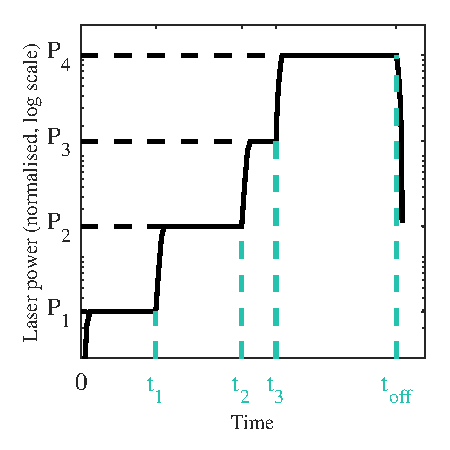
\includegraphics[width=.45\textwidth]{figures/LowCR/LaserProfile_half.eps}}
\subfigure b){\label{fig:CapsuleDesign}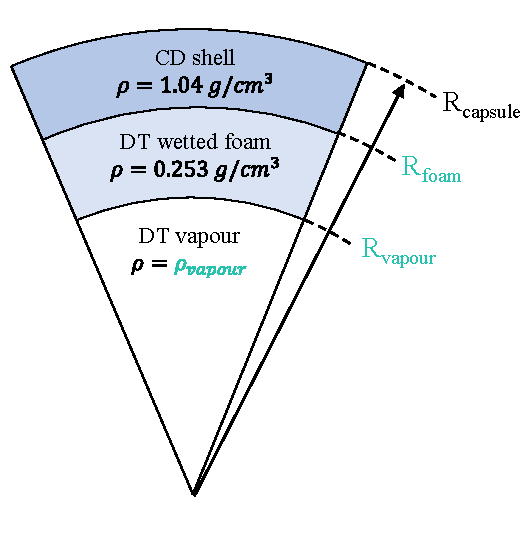
\includegraphics[width=.45\textwidth]{figures/LowCR/Capsule.pdf}}
\caption{Plots of a) the laser profile and b) the capsule design. The laser sequence consists of a laser being applied at the start of the simulation, leading to four pulses of increasing power. The power begins to increase at the times $t_1, t_2$ and $t_3$ (with a linear rise over 200 \unit{\pico\second}), and the laser is switched off at time $t_{off}$ (with a linear decay over 200 \unit{\pico\second}). The capsule has three layers, with material interfaces at  $R_{vapour}$ and $R_{foam}$ and an outer radius of $R_{capsule}$. When optimising this design, $R_{capsule}$ is selected and considered fixed. This is used to define the laser pulse powers $P_1, P_2, P_3$ and $P_4$, which are also not changed. This leaves seven optimisation parameters, which are indicated in teal: $t_1, t_2, t_3, R_{vapour}, R_{foam}$ and $\rho_{vapour}$ (the DT vapour density).}
\end{figure}

The simulation campaign involved optimising a series of capsule within the low-instability regime defined by the four instability criteria. To perform this optimisation, a laser pulse-profile and capsule were designed, with a number of parameters that could be varied between simulations. In this section, the design of this capsule and pulse-profile are described, and the optimisation parameters identified.

The capsule used for the simulations, displayed in Figure \ref{fig:CapsuleDesign}, was a simple three layer design consisting of a central DT-vapour region surrounded by a DT-wetted-foam layer and a deuterated plastic (CD) ablator. The simulation campaign actually consisted of a number of smaller optimisation campaigns for capsules of different outer radius; an outer radius was selected, and then the capsule and implosion were optimised with the outer radius considered a fixed parameter. During this optimisation, the interior dimensions of the capsule ($R_{vapour}$ and $R_{foam}$) were varied, and the density in the vapour region ($\rho_{vapour}$) was varied over the 0.6 \unit{\milli\gram\per\centi\meter\cubed} $< \rho_foam <$ 4.0 \unit{\milli\gram\per\centi\meter\cubed} range achievable with wetted-foam capsules. The wetted-foam layer had a fixed density of 0.253 \unit{\gram\per\centi\meter\cubed}, while the ablator had a density of 1.04 \unit{\gram\per\centi\meter\cubed}. This simple capsule design can be easily optimised, but is also a realistic design similar to those used in experiments\footnote{ The use of a central vapour region surrounded by a dense fuel layer is standard for ignition designs, but the choice of ablator can vary: these can include the use of HDC rather than plastic \cite{Mackinnon2014}, or can contain layers of dopants (such as silicon) to absorb hot-electrons and thus minimise preheating \cite{Solodov2022}.}. 

The laser pulse profile, displayed in Figure \ref{fig:LaserProfile}, consisted of a series of `steps' of constant laser power with a 0.2 \unit{\nano\second} linear rise time between each step. A 351 \unit{\nano\meter} nm laser was used, corresponding to the third-harmonic of Nd:glass. Both three- and four-pulse profiles were considered. The timings of each step ($t_1, t_2$ and $t_3$ in the figure) were treated as optimisation parameters, along with the time at which the laser was switched off ($t_off$). The relative laser powers were fixed and were not changed during the optimisation (the maximum power for the particular capsule radius was calculated from the intensity criteria, and the pulse profile was scaled accordingly). The pulse-powers were chosen to roughly reduce the amount of entropy injected into the fuel, and the overall design was chosen to be simple to implement and optimise, while also being feasible on current facilities. Ideally the pulse powers would also have been optimised, but adding an extra four optimisation variables was deemed to be infeasible.

The three laser timings, laser switch off time, internal capsule radii and DT vapour density resulted in seven optimisation parameters. During each optimisation, the capsule outer radius was selected and kept constant; this also defined the pulse powers. Simulations were then performed to identify the parameters of these seven variables giving the maximum possible yield while satisfying all four instability criteria. Since the capsule radius also defined the laser power and the approximate implosion time, it also defined a rough energy for the implosion to be optimised.


\section{Performing the simulation campaign} \label{sec: OptimisationCampaign}

\subsection{The simulation code HYADES}

The 1D Lagrangian radiation hydrodynamics code HYADES was used for this simulation campaign.  HYADES was developed and is supplied through Cascade inc., and for the purposes of this work was ran on the SCARF supercomputer at the UKRI-STFC Rutherford Appleton Laboratory. It had previously been used for other large-scale simulation campaigns of ICF implosions \cite{Hatfield2019}. 

HYADES contains a number of different options for the various physics models. Those used in these simulations were based on the advice and recommendations of Dr Robbie Scott at the CLF. For this work, an average-atom LTE ionisation model was used, with a multi-group radiation diffusion approximation was used for radiation transport. A multiplier of 0.8 was also applied to the input laser energy to account for losses (such as those due to cross-beam energy transfer). A series of benchmarking simulations were performed after the main campaign to confirm that these settings were sufficient to describe experimental shots; theses are described in the appendix.

The DT vapour regions were described in the simulations using the in-line HYADES QEOS model, while the thin plastic shell was described as deuterated plastic and used the SESAME EOS table for CH. These are the standard, accepted ways of describing these materials. The wetted foam layer was less well-described, as no equation of state table for DT wetted foam was available. Instead, the DT wetted-foam layer was described as a conventional DT ice layer, described by the same DT QEOS model as for the DT vapour. The simulation therefore does not include the presence of the foam. This is a limitation of this work which is discussed further in later sections.

\subsection{Capsule meshing}

HYADES does not have an in-built meshing routine, and thus a meshing script had to be produced to allow different targets to be simulated. This mesh has two major requirements to ensure accuracy; the resolution of the mesh at the capsule outer edge should be sufficiently high, and the relative mass difference between zones should not be much greater than $\sim$ 2\%. In addition to this, an increased number of zones/mesh points leads to an increased simulation time, and thus it is desirable to keep the number of zones to a minimum while satisfying these two conditions.

A custom meshing routine was written for this simulation campaign. This routine was automatic and robust, allowing meshes to be created to describe capsules of a range of different sizes and layer thicknesses relevant to this investigation. The production of such a meshing algorithm was essential to being able to perform the large parameter scans that were the main feature of this work, as it enabled large numbers of capsules with different structures to be simulated with accuracy. The principles of this code (along with the underlying theory) is outlined in Appendix \ref{app:KeyCode}.

The meshing algorithm produced worked sufficiently well for the campaign to be conducted. It operated less well as the thicknesses of the layers began to vary too drastically, but this did not prevent the optimisations being performed; if the thicknesses had changed drastically enough that for the meshing code to stop working well, the performance had always decreased to such an extent that it was clearly not worth investigating, or the criteria for implosion velocity/IFAR would have been exceeded. However, if simulations of drastically different designs were required, a new and more robust meshing algorithm would need to be developed.

\subsection{Conducting the simulation campaign}

The overall simulation campaign consisted of a number of smaller campaigns, each optimising a different capsule outer radius (and thus producing an implosion at a different energy). For each campaign, a rough initial simulation was created with reasonable initial parameters. Large parameter scans were then performed varying either the two layer thicknesses, or two of the three laser timings, over the course of around 100 simulations. The results of these would then be analysed on a series of plots considering the gain, convergence ratio, implosion velocity and IFAR as a function of the input parameters. Trends in these parameters were identified, and the simulations giving the optimal balance of yield and the instability criteria selected. A new round of simulations would then be performed varying further parameters, and the process repeated. This was an iterative process - optimising the laser timings would then often lead to a new optimal thickness, which in turn would lead to a change in the optimal laser timings again. This process was repeated until it stopped yielding capsules with better performance.

Througout this optimisation, the results would be monitored and the vapour density would also be investigated. For instance, if there were a number of capsules with lower yield than the current `optimal' design, but which also had a much lower convergence ratio than the limit of 16, then the vapour pressure would be reduced - this would increase the CR and gain of these capsules, and may result in them outperforming the previous best result. Equally, if a large number of the capsules satisfied the other criteria but the convergence ratio was too high, the vapour density would be reduced. This led to multiple repeats of the same round of optimisation at different vapour densities.

The time at which the laser was turned off was also treated separately from the other optimisation parameters. In all ICF implosions, there is a point after the peak implosion velocity is achieved at which the laser accelerates the shell no further. After this point, there is no benefit to applying the laser in terms of fusion performance - but doing so will increase the input energy, and thus decrease the gain. This effect could be substantial, and trends in the gain were being obscured based on how long after this point the laser was applied for. To resolve this, the laser was applied until the end of the each simulation, and the gain calculation was adjusted so that only the laser energy used up until the bang time was included in the calculation. This meant that the influence of this laser switch-off time was removed. Once the implosion had otherwise been optimised, the laser switch off-time would then be varied and the true gain (using the full applied laser energy) would be calculated; this would reveal a clear optimal value, and this would then be reported as the final gain and optimised implosion.

Care was also taken to ensure that appropriate time resolution was being used in all simulations, and that the simulation end time was appropriate. If the simulation ended before the capsule had properly converged, the gain would inevitably be too low. This could typically be spotted by unfeasible data (for instance, a very low convergence ratio). To test for this, a representative number of the simulations would be analysed individually to check that the full behaviour was being captured, and that the simulations looked appropriate.

This procedure generated the `optimal' design for a particular capsule radius, and a particular number of laser pulses. The procedure was repeated multiple times to generate optimal 3-pulse and 4-pulse sequences for a range of different capsule radii.

\subsection{Hydroscaling}

When this campaign was first conducted (in 2020) it was done from first principles for each capsule to minimise the number of assumptions on the optimal implosion. However, it was clear that all the capsules had comparable relative thicknesses and timings. In 2022, a further optimisation was performed to fill in a gap in the energies investigated, and this time hydrocaling relations were applied to produce an initial capsule from which to start the optimisation. This significantly reduced the rounds of simulations required to achieve convergence.

Hydroscaling makes use of the fact that much of the physics in an ICF implosion (particularly in 1D) is scale independent, and thus many of the parameters scale in a straightforward manner with capsule size. These relations state that $t \propto R \propto E^{1/3}$ where $t$ and $R$, are the implosion timings (including all laser timings) and capsule radii (including all internal boundaries) respectively, and $E$ is the laser energy \cite{Nora2014}. This meant that, based on the energy desired for the implosion, a rough estimate could be produced of the necessary capsule size. The interior dimensions of the capsule could be scaled accordingly, as could the laser timings. This was then used as the starting point of the optimisation to produce a capsule that already had a good level of fusion performance, which was then further increased by the optimisation.

\section{Results and analysis} \label{sec: LowCRResults}

Over 20,000 simulations were performed in total, with over 10,000 satisfying all four instability criteria; these $\sim$10,000 valid simulations are plotted as a function of gain vs laser energy in Figure \ref{fig:loglog}. The data can be seen to form eight rough peaks, corresponding to the eight different outer radii (and thus energy scales) considered. The four-pulse laser sequences are displayed in black, while the three-pulse sequences are displayed in teal. As expected, the lower adiabat four-pulse sequences outperformed the three-pulse sequences at all energy scales. The best performing three-pulse and four-pulse simulation for each capsule size has been tabulated in Table \ref{tab:ThirdHarmonic}. 

\begin{figure}[ht!]
\centering
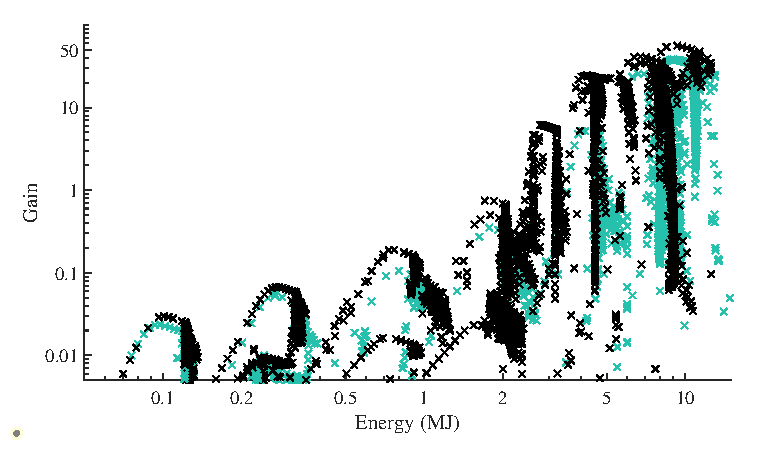
\includegraphics{figures/LowCR/AllData_full.eps}
\caption{A log-log plot showing the simulated gain vs input energy, for the simulations where the criteria to minimise instabilities were satisfied. Simulations where a 3-pulse sequence was used are represented by a red/grey point, whilst those using 4-pulse sequences are coloured blue/black. Nine groupings of points are visible, corresponding to the nine different capsule sizes used.}
\label{fig:loglog}
\end{figure}


\begin{table}
\resizebox{\textwidth}{!}{%
  \centering
\begin{tabular}{|c|c|c|c|c|c|c|c|c|}
\hline
 Number of pulses & \multicolumn{8}{c|}{3} \\
 \hline
 Size multiplier & 0.25 & 0.35 & 0.5 & 0.65 & 0.75 & 0.85 & 1 & 1.1 \\ 
\hline
Laser energy (MJ) & - & - & 0.80 & 1.8 & - & 4.0 & 6.6 & 8.9\\ 
Gain & - & - & 0.11 & 0.35 & - & 5.2 & 26 & 38\\ 
Convergence ratio & - & - & 15.3 & 15.5 & - & 15.9 & 16.0 & 16.0\\ 
IFAR & - & - & 20.3 & 18.7 & - & 15.2 & 14.3 & 12.7 \\ 
Implosion velocity (km/s) & - & - & 399.2 & 395.4 & - & 373.9 & 358.4 & 332.4\\ 
Max pulse power (TW) & - & - & 173.00 & 292.38 & - & 500.12 & 692.13 & 837.50\\ 
Pulse 2 switch on time (ns) & - & - & 3.65 & 3.80 & - & 5.00 & 6.20 & 7.00\\ 
Pulse 3 switch on time (ns) & - & - & 4.15 & 4.90 & - & 6.30 & 7.60 & 8.80\\ 
Laser switch off time (ns) & - & - & 8.50 & 10.50 & - & 13.75 & 16.50 & 18.60\\ 
Vapour/liquid boundary (\si[per-mode=symbol]{\milli\meter}) & - & - & 1.3000 & 1.6835 & - & 2.2100 & 2.6100 & 2.8710\\ 
Liquid/CD boundary (\si[per-mode=symbol]{\milli\meter}) & - & - & 1.4000 & 1.8200 & - & 2.3800 & 2.7900 & 3.0580\\ 
Outer radius (\si[per-mode=symbol]{\milli\meter}) & - & - & 1.4250 & 1.8525 & - & 2.4225 & 2.8500 & 3.1350\\ 
Vapour density (\si[per-mode=symbol]{\milli\gram\per\centi\meter\cubed}) & - & - & 1.00 & 0.85 & - & 0.65& 0.65 & 0.70\\
\hline

Number of pulses & \multicolumn{8}{c|}{4} \\
\hline
Size multiplier & 0.25 & 0.35 & 0.5 & 0.65 & 0.75 & 0.85 & 1 & 1.1 \\ 
\hline
Laser energy (MJ) & 0.10  & 0.27 & 0.77 & 1.7 & 2.8 & 4.2 & 6.7 & 8.5\\ 
Gain & 0.030 & 0.067 & 0.19 & 0.75 & 6.1 & 24 & 42 & 54\\ 
Convergence ratio & 15.7 & 15.7 & 16.0 & 15.8 & 16.0 & 15.9 & 16.0 & 15.7\\ 
IFAR & 23.4 & 27.5 & 29.7 & 25.1 & 23.8 & 21.2 & 18.4 & 15.7\\ 
Implosion velocity (km/s) & 391.4 & 395.8 & 399.6 & 399.6 & 387.8 & 347.5 & 334.1 & 311.0\\ 
Max pulse power (TW) & 43.26 & 84.79 & 173.00 & 292.38 & 389.36 &500.12 & 692.13 & 837.50\\ 
Pulse 2 switch on time (ns) & 1.10 & 2.20 & 2.60 & 3.60 & 4.20 & 3.70 & 5.20 & 5.70\\ 
Pulse 3 switch on time (ns) & 3.00 & 4.60 & 5.60 & 7.80 & 8.80 & 9.40 & 12.80 & 15.00\\ 
Pulse 4 switch on time (ns) & 3.60 & 5.50 & 6.80 & 9.50 & 10.90 & 11.40 & 15.30 & 18.00\\ 
Laser switch off time (ns) & 5.80 & 8.50 & 11.00 & 15.00 & 17.65 & 19.40 & 24.50 & 27.50\\ 
Vapour/liquid boundary (\si[per-mode=symbol]{\milli\meter}) & 0.6325 & 0.8950 & 1.3050 & 1.6705 & 1.9275 & 2.2100 & 2.6000 & 2.8270\\ 
Liquid/CD boundary (\si[per-mode=symbol]{\milli\meter}) & 0.69625 & 0.976 & 1.3950 & 1.8200 & 2.1000 & 2.3630 & 2.7800 & 3.0580\\ 
Outer radius (\si[per-mode=symbol]{\milli\meter}) & 0.7125 & 0.9975 & 1.4250 & 1.8525 & 2.1375 & 2.4225 & 2.8500 & 3.1350\\ 
Vapour density (\si[per-mode=symbol]{\milli\gram\per\centi\meter\cubed}) & 1.35 & 1.35 & 1.05 & 1.00 & 0.90 & 0.85 & 1.00 & 1.00\\
\hline
\end{tabular}}
\caption{Simulation parameters used to achieve the maximum gains for each capsule size for both pulse sequences. The original capsule was the column with size multiplier of 1. New capsule sizes (and thus energy scales) were simulated by multiplying the radius by the size multiplier. In order to keep $I\lambda^2$ constant over different capsule sizes, the pulse powers were then multiplied by the square of the size multiplier. Gain is given to two significant figures, whilst convergence ratio, IFAR and implosion velocity are given to one decimal place. This level of precision is higher than would typically be quoted for a 1D simulation, but is used here to indicate how the values compare with the imposed limits. While convergence ratio is in places displayed as 16.0, the value to the precision calculated in the analysis is below this upper limit. The original simulation campaign was performed for five capsule sizes; three further sizes (0.25, 0.35 and 0.75) were performed later, but only four pulse sequences were optimized.}
\label{tab:ThirdHarmonic}
\end{table}

These results demonstrate that high reactor-level gains can be achieved in this conservative regime, with a gain of 54 being achieved for an energy of 8.5 \unit{\mega\joule}. However, this is a much higher energy than is currently achievable, and is likely too high for an economically viable fusion reactor - suggesting that a fusion reactor could not be constructed using this particular approach. However, the lower energy performance is interesting. The gains of 0.19 and 0.75 at 0.77 \unit{\mega\joule} and 1.7 \unit{\mega\joule} respectively are impressive given the conservative nature of this regime. It is also worth noting that when this work was performed the record ICF gain was 0.03, and so this result suggested an improvement (at the time) of an order of magnitude. Recent developments have led to higher gains, but this suggests that comparable performance can be achieved in a conservative regime, where instability growth is less of a concern (and implosions would hopefully be robust). The recent NIF results (a gain of 0.7 at 1.9 MJ, and a gain of 1.5 at 2.05 MJ) actually fit just below the trend of this data (this is plotted in Figure \ref{fig:ArF and Two colour} in the following chapter), suggesting that the performance of the current best shots is comparable to what is predicted here.

The conditions in the hotspot and shell of the 0.77 \unit{\mega\joule} capsule are displayed in \ref{fig:HSandShellLMJ}. It can be seen that the hotspot conditions are close to that required for ingition. The areal density is greater than the 0.3 \unit{\gram\per\centi\meter\squared} commonly quoted as required for ignition to occur, but the ion temperature (just below 4 keV) is slightly too low. This suggests that ignition could be within reach, if it was possible to increase this ion temperature just prior to the bang-time. This is investigated further in Chapter \ref{ch-FurtherSims}. It is also interesting to note the relatively low areal density of the shell, which arises from the limited convergence of the capsule. This is most easily increased in this regime by increasing the size of the capsule.

It is useful to note again here the purpose of this work, which is not to claim that these exact gains are possible - these are the results of 1D simulations only, and thus can not be expected to be fully accurate. However, the expected low-instability growth means that such simulations are expected to be a more representative estimate of performance than would otherwise be the case, and thus should be sufficient to give a good first-estimate of potential experimental performance. Overall, these results show that it may indeed be possible to achieve interesting fusion performance (comparable to the current best-performing shots on the NIF) in this conservative regime, based around low-convergence ratio and where performance is expected to be minimal.

\begin{figure}[ht]
\centering
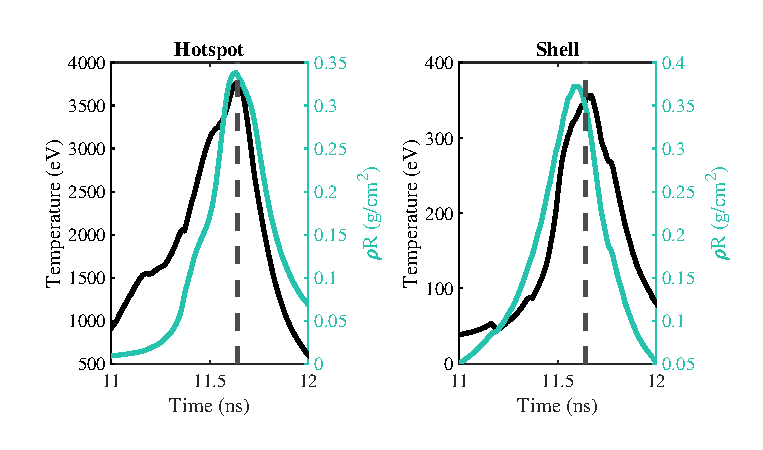
\includegraphics{figures/LowCR/RhoRandT.eps}
\caption{A log-log plot showing the simulated gain vs input energy, for the simulations where the criteria to minimise instabilities were satisfied. Simulations where a 3-pulse sequence was used are represented by a red/grey point, whilst those using 4-pulse sequences are coloured blue/black. 5 groupings of points are visible, corresponding to the five different capsule sizes used.}
\label{fig:HSandShellLMJ}
\end{figure}


\section{Limitations and suggested future work} \label{sec: LowCRLimitations}
There are a number of limitations of this work, some of which will be investigated further in the following chapters. These limitations also suggest potential avenues for future research.

Firstly, the fundamental limitation of this work is the use of 1D simulations. While the effort made here to define a low-instability regime means that 1D like-behaviour is expected, this is still a fundamental assumption upon which this work relies. While 1D simulations are sufficient for an initial investigation of the regime as has been conducted here, to explore it with greater confidence simulations in higher dimensions are required. We have recently secured access to the University of Rochester's RIGEL code, and plan to use this for confirmatory 2D simulations.

Secondly, the direct-drive nature of this work coupled with the high laser energies makes experimental verification of the regime challenging. When this work was performed, the use of cryogenic targets and the high energies meant that performing shots based on these designs would not be possible, due to a lack of cryogenic capabilities for direct-drive shots at the NIF \cite{Hohenberger2015}. Fortunately this has since been rectified, and direct-drive shots of wetted-foam targets are being planned. However, this still requires cryogenic shots on the NIF, which makes limits the opportunity to test this regime. An alternative solution to this is proposed in the next chapter. In addition, such shots would need to be performed in a PDD configuration. This is contrary to these simulations, where fully symmetric direct-drive was assumed (and the benchmarking simulations in Appendix \ref{app:benchmark} suggest that a reduced laser input multiplier would potentially be required to describe PDD shots).

Thirdly, the simulations make a number of approximations that are not particularly accurate, which likely lead to some over-estimation of the performance. The two main ones are as follows: 1) the laser in the 1D simulations is focussed at the centre of the capsule, which means that it remains perfectly focused as the capsule implodes. This is unphysical. However, the benchmarking simulations in Appendix \ref{app:benchmark} suggest that the input multiplier used to account for this is reasonable for in the case of a spherical direct-drive implosion, although a lower multiplier may be required for a polar direct drive setup. 2) The description of the wetted foam as simply a DT layer (with the CH foam not accounted for) is a poor one, and is only valid if the foam density is below $\sim10$~\si[per-mode=symbol]{\milli\gram\per\centi\meter\cubed} \cite{CHFoamLim}. Other groups have used a less-compressible mixed CH + DT equation of state to describe this material with more accuracy \cite{Olson2021}; this is investigated in the following section. This is further complicated by the fact that the equation of state for even dry foams at these low densities are not well simulated, which motivated the experiment in later chapters. Further study is required to better describe this material if wetted-foams are to be simulated to higher accuracy, and ultimately experiments to measure the wetted foam equation of state are required; this is enough topic that we are continuing to investigate.

In addition, while these are presented as `optimisation' campaigns, exploring such large parameter spaces manually is incredibly difficult, and thus no guarantee can be made that optimal performance has been obtained. This approach would be well-suited to a machine learning approach, which could automate the optimisation process and hopefully explore the parameter space more efficiently. Machine-learning has been applied to ICF for similar problems in the past successfully \cite{Hatfield2019}, and this is something that we are currently investigating within our research group. If this could be done successfully, it would allow many more simulation campaigns to be performed of this ilk with relative ease. The impact of more parameters could be explored (for example, the laser pulse powers), and the criteria applied to limit the parameter space could be adjusted (i.e. to investigate alternative maximum implosion velocities) or to include other parameter (for instance, applying a minimum permitted adiabat).

In addition, while the regime identified is expected to be result in low-instability growth, there are other parameters which could be included to increase confidence in this. The most obvious would be the adiabat of the implosion. In addition, no limit was placed on the strength of the first shock, as the impact of particular asymmetry seeds was not considered in this work. This is a significant limitation, since the strength of the first shock has been shown to be key to mitigating instabilities from the support tent (in indirect implosions) and ablator micro-structure. If future simulation campaigns were to be performed (particularly if machine learning was to be applied), repeating this campaign with a 10 Mbar first shock should be a priority.

\section{Conclusion} \label{sec:LowCRConclusions}
A simulation campaign to investigate the performance of wetted-foam capsules in a low-instability regime was presented, where the regime is defined by low convergence ratio, IFAR, implosion velocity, and laser intensity. While the laser energy necessary for an IFE reactor based on this approach is not feasible, the performance at lower energies is comparable to the recent record shots on the NIF. This suggests that substantial fusion performance can be obtained despite the conservative approach taken here, and that further exploration of this regime could be interesting. A variety of potential extensions and improvements to this work have been suggested, many of which are explored in the following chapter.

This chapter has also demonstrated the utility of such an optimisation campaign - a general platform which can be used to explore fusion performance in a particular parameter space. This approach has again been applied in the subsequent chapter to explore variations on the implosion scheme discussed here.





















%\begin{table}[t]
%\resizebox{\textwidth}{!}{%
%\centering
%\begin{tabular}{|c|c|c|c|c|c|c|}
%\hline
% Number of pulses & \multicolumn{6}{c|}{3} \\
% \hline
% Size multiplier & 0.5 & 0.65 & 0.75 & 0.85 & 1 & 1.1 \\ 
%\hline
%Laser energy (MJ) & 0.80 & 1.8 & - & 4.0 & 6.6 & 8.9\\ 
%Gain & 0.11 & 0.35 & - & 5.2 & 26 & 38\\ 
%Convergence ratio & 15.3 & 15.5 & - & 15.9 & 16.0 & 16.0\\ 
%IFAR & 20.3 & 18.7 & - & 15.2 & 14.3 & 12.7 \\ 
%Implosion velocity (km/s) & 399.2 & 395.4 & - & 373.9 & 358.4 & 332.4\\ 
%Max pulse power (TW) & 173.00 & 292.38 & - & 500.12 & 692.13 & 837.50\\ 
%Pulse 2 switch on time (ns) & 3.65 & 3.80 & - & 5.00 & 6.20 & 7.00\\ 
%Pulse 3 switch on time (ns) & 4.15 & 4.90 & - & 6.30 & 7.60 & 8.80\\ 
%Laser switch off time (ns) & 8.50 & 10.50 & - & 13.75 & 16.50 & 18.60\\ 
%Vapour/liquid boundary (\si[per-mode=symbol]{\milli\meter}) & 1.3000 & 1.6835 & - & 2.2100 & 2.6100 & 2.8710\\ 
%Liquid/CD boundary (\si[per-mode=symbol]{\milli\meter}) & 1.4000 & 1.8200 & - & 2.3800 & 2.7900 & 3.0580\\ 
%Outer radius (\si[per-mode=symbol]{\milli\meter}) & 1.4250 & 1.8525 & - & 2.4225 & 2.8500 & 3.1350\\ 
%Vapour density (\si[per-mode=symbol]{\milli\gram\per\centi\meter\cubed}) & 1.00 & 0.85 & - & 0.65& 0.65 & 0.70\\
%\hline

%Number of pulses & \multicolumn{6}{c|}{4} \\
%\hline
%Size multiplier & 0.5 & 0.65 & 0.75 & 0.85 & 1 & 1.1 \\ 
%\hline
%Laser energy (MJ) & 0.77 & 1.7 & 2.8 & 4.2 & 6.7 & 8.5\\ 
%Gain & 0.19 & 0.75 & 6.1 & 24 & 42 & 54\\ 
%Convergence ratio & 16.0 & 15.8 & 16.0 & 15.9 & 16.0 & 15.7\\ 
%IFAR & 29.7 & 25.1 & 23.8 & 21.2 & 18.4 & 15.7\\ 
%Implosion velocity (km/s) & 399.6 & 399.6 & 387.8 & 347.5 & 334.1 & 311.0\\ 
%Max pulse power (TW) & 173.00 & 292.38 & 389.36 &500.12 & 692.13 & 837.50\\ 
%Pulse 2 switch on time (ns) & 2.60 & 3.60 & 4.20 & 3.70 & 5.20 & 5.70\\ 
%Pulse 3 switch on time (ns) & 5.60 & 7.80 & 8.80 & 9.40 & 12.80 & 15.00\\ 
%Pulse 4 switch on time (ns) & 6.80 & 9.50 & 10.90 & 11.40 & 15.30 & 18.00\\ 
%Laser switch off time (ns) & 11.00 & 15.00 & 17.65 & 19.40 & 24.50 & 27.50\\ 
%Vapour/liquid boundary (\si[per-mode=symbol]{\milli\meter}) & 1.3050 & 1.6705 & 1.9275 & 2.2100 & 2.6000 & 2.8270\\ 
%Liquid/CD boundary (\si[per-mode=symbol]{\milli\meter}) & 1.3950 & 1.8200 & 2.1000 & 2.3630 & 2.7800 & 3.0580\\ 
%Outer radius (\si[per-mode=symbol]{\milli\meter}) & 1.4250 & 1.8525 & 2.1375 & 2.4225 & 2.8500 & 3.1350\\ 
%Vapour density (\si[per-mode=symbol]{\milli\gram\per\centi\meter\cubed}) & 1.05 & 1.00 & 0.90 & 0.85 & 1.00 & 1.00\\
%\hline
%\end{tabular}}
%\caption{Simulation parameters used to achieve the maximum gains for each capsule size for both pulse sequences. The original capsule was the column with size multiplier of 1. New capsule sizes (and thus energy scales) were simulated by multiplying the radius by the size multiplier. In order to keep $I\lambda^2$ constant over different capsule sizes, the pulse powers were then multiplied by the square of the size multiplier. Gain is given to two significant figures, whilst convergence ratio, IFAR and implosion velocity are given to one decimal place. This level of precision is higher than would typically be quoted for a 1D simulation, but is used here to indicate how the values compare with the imposed limits. While convergence ratio is in places displayed as 16.0, the value to the precision calculated in the analysis is below this upper limit.}
%\label{tab:ThirdHarmonic}
%\end{table}

%\begin{table}[t]
%\centering
%\begin{tabular}{|c|c|c|c|}
%\hline
%Number of pulses & \multicolumn{3}{c|}{4} \\
%\hline
%Size multiplier & 0.25 & 0.35 & 0.75 \\ 
%\hline
%Laser energy (MJ) & 0.10  & 0.27  & 2.8\\ 
%Gain & 0.030 & 0.067 &  6.1\\ 
%Convergence ratio & 15.7 & 15.7 &  16.0\\ 
%IFAR & 23.4 & 27.5 & 23.8\\ 
%Implosion velocity (km/s) & 391.4 & 395.8 & 387.8\\ 
%Max pulse power (TW) & 43.26 & 84.79 & 389.36\\ 
%Pulse 2 switch on time (ns) & 1.10 & 2.20 & 4.20\\ 
%Pulse 3 switch on time (ns) & 3.00 & 4.60 & 8.80\\ 
%Pulse 4 switch on time (ns) & 3.60 & 5.50 & 10.90\\ 
%Laser switch off time (ns) & 5.80 & 8.50 & 17.65\\ 
%Vapour/liquid boundary (\si[per-mode=symbol]{\milli\meter}) & 0.6325 & 0.8950 & 1.9275\\ 
%Liquid/CD boundary (\si[per-mode=symbol]{\milli\meter}) & 0.69625 & 0.976 & 2.1000\\ 
%Outer radius (\si[per-mode=symbol]{\milli\meter}) & 0.7125 & 0.9975 & 2.1375\\ 
%Vapour density (\si[per-mode=symbol]{\milli\gram\per\centi\meter\cubed}) & 1.35 & 1.35 & 0.90\\
%\hline
%  \end{tabular}
%\caption{Simulation parameters used to achieve the maximum gains for three further capsules. These optimisations were done after the main campaign. The three-pulse sequences for these capsules were not fully optimised, and so have not been tabulated.}
%\label{tab:ThirdHarmonic_2}
%\end{table}
%\begin{savequote}[8cm]
%Alles Gescheite ist schon gedacht worden.\\
%Man muss nur versuchen, es noch einmal zu denken.

%All intelligent thoughts have already been thought;\\
%what is necessary is only to try to think them again.
 % \qauthor{--- Johann Wolfgang von Goethe \cite{von_goethe_wilhelm_1829}}
%\end{savequote}

\chapter{\label{ch-FurtherSims} Further simulation campaigns in the low-CR regime}

\minitoc

\section{Introduction}
The previous chapter had three key results. Firstly, this new expected low-instability regime was defined, where 1D simulation is expected to provide a reasonable estimate of performance. Secondly, the performance of conventional hot-spot implosions of wetted-foam capsules using third-harmonic laser light was explored and well-characterised. Finally, the code and methodology for this style of optimisation campaign was established.

In this chapter, these previous results will be built upon through further simulation.  In Section \ref{sec:MixedEOS}, the impact of the EOS model used to describe the wetted-foam is investigated, in an attempt to address one of the limitations noted at the end of the previous chapter. One of the other limitations mentioned of this approach was the difficulty of verifying this regime experimentally, and so in Section \ref{sec:Hydroequivalent} a new surrogate target (the `hydrodynamic equivalent' capsules) are proposed and optimised to allow room temperature experiments.

In the second half of the chapter, further simulation campaigns are performed to explore how new techniques could be applied within the low-instability regime to further increase fusion performance. In Section \ref{sec:AlternativeDrivers} the potential performance benefits of using higher frequency lasers are investigated, through additional implosion optimisations. Finally, in Section \ref{sec:AuxiliaryHeating}, an auxiliary heating scheme using electron beams is discussed and applied to the previous simulations.

\subsection{An alternative fusion metric: the burning plasma parameter}
It is relevant at this stage to introduce an additional fusion metric, which will be used later in this chapter (in particular in Section \ref{sec:AuxiliaryHeating}) to evaluate fusion performance. So far in this thesis gain has been the primary fusion metric, but this measure of performance has some limitations for this particular work. Gain requires the input energy of the implosion to be known, which this is not the case in Section \ref{sec:AuxiliaryHeating} where the energy required for the auxiliary heating is not known to high accuracy. This dependence on input energy means that an identical implosion will therefore appear more/less successful in terms of gain depending on the efficiency with which it can be driven. As such, it is useful to introduce alternative metrics that do not suffer from this.

Therefore, a metric known as the `burning plasma parameter' is used. The version used here - the `total capsule burning plasma parameter' - is defined as 
\begin{equation} Q^\mathrm{{tot}}_{\mathrm{\alpha}} = \frac{1}{2} \frac{E_\mathrm{\alpha}}{ E^\mathrm{{tot}}_{\mathrm{PdV}}}, \label{eqn:Qtot defn} \end{equation} where $E_\mathrm{\alpha}$ is the alpha particle energy deposited back into the hotspot over the total duration of the implosion, and $E^\mathrm{{tot}}_{\mathrm{PdV}}$ is the total work done on the capsule hotspot and shell at the time of stagnation (maximum pressure) \cite{Betti2015}. This metric compares the energy absorbed from alpha self heating at the bang time of the capsule to the external energy used to compress the capsule; the burn is assumed to be symmetric around the bang time, such that the alpha self-heating at the bang time is equal to half of the total alpha heating $E_\mathrm{\alpha}$ (explaining the factor half in the formula). 

A value of $Q^\mathrm{{tot}}_{\mathrm{\alpha}} > 1$ defines the `burning plasma' regime, where more alpha heating is the dominant source of energy in the capsule \cite{Christopherson2020}. The burning plasma parameter is therefore a useful metric for fusion capsules, as it provides direct information about the energetics of the implosion. It does not depend on input energy, and thus how efficiently the capsule is driven; this makes it ideal for analysing the auxiliary heating capsule, as unlike gain it is not influenced by factors such as how efficiently the electron beams could be generated (which are independent of the implosion).

An early rough indicative estimate for ignition based on the burning plasma parameter was set at $Q^\mathrm{{tot}}_{\mathrm{\alpha}} = 10$, where the cumulative alpha heating at the bang-time is ten times greater than the work done on the hot spot and shell \cite{Betti2011}. However, it should be noted that there is a subtly different variant of the burning plasma parameter, known as the `hotspot burning plasma parameter', where the total work done on the whole capsule $E^\mathrm{{tot}}_{\mathrm{PdV}}$ is instead replaced by the total work done on the hotspot only, and the value is typically around twice as large \cite{Betti2015}. An alternative ignition criteria has been proposed based on this parameter \cite{Christopherson2020}, where $Q^\mathrm{{hs}}_{\mathrm{\alpha}} > 1.4$ is treated as the threshold. This definition treats ignition as the the point at which self-heating results in burn propagation through the cold shell (demonstrating the ambiguity surrounding ignition discussed in Chapter \ref{ch:definitions}).

\section{Estimating the impact of the wetted-foam EOS} \label{sec:MixedEOS}

The HYADES simulations used in this thesis are intended to describe wetted-foam targets, but in reality this layer is described using the pure-DT equation of state. This approximation does not account for the presence of the foam material, and this was highlighted as a limitation of this work in the previous chapter. There is no wetted-foam equation of state that is currently generally available. Other work (at US national labs) has used a mixed equation of state, which does include the presence of the foam \cite{Olson2021}; this is reported to be less compressible than pure-DT, resulting in a thicker but less dense shell and a reduced fusion yield.

A variety of attempts were made to estimate the impact that an improved equation of state might have on the implosions presented in the previous chapter. In this section, the results of simulations using the 1D radiation-hydrodynamic code HELIOS are presented \cite{MacFarlane2006}. Unlike HYADES, HELIOS does not include alpha-deposition; alpha particles generated in fusion reactions cannot be reabsorbed, and thus ignition is not possible. HELIOS can be used with an additional program, PropacEOS, which allows equation of state tables to be generated based on material composition. These PropacEOS tables can then be used in Helios for the material. This program was used to produce a wetted-foam EOS table, by assuming that such a foam was made of a 2\% atomic fraction of carbon, 48\% tritium, and 50\% tritium (corresponding to a 25 \unit{\milli\gram\per\centi\meter\cubed} deuterated plastic foam, saturated with a 50:50 mix of liquid DT).

\begin{figure} 
	\centering     %%% not \center
	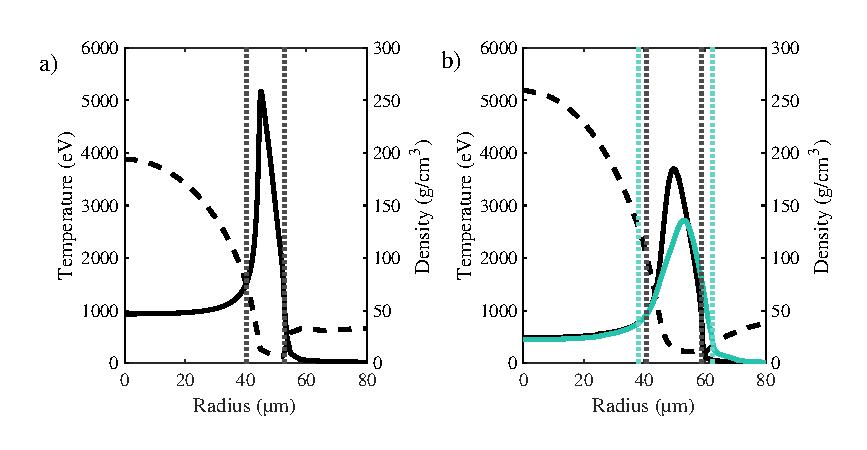
\includegraphics[width=.8\textwidth]{figures/FurtherSims/MixedEOS.eps}
	\caption{\label{fig:MixedEOS} Temperature (dashed lines) and density (solid line) at the bang time for a) the 0.25 size 4-pulse implosion simulated in HYADES, and b) the same simulation in HELIOS. In b), the teal solid line represents the density profile for the same simulation when a mixed-EOS is used (the temperature profiles for these two simulations overlap). The dotted vertical lines show the hotspot and shell boundaries (where again, the dotted teal lines refer to the mixed-EOS). )}
\end{figure}

\begin{table}
	\centering
	\begin{tabular}{|c|c|c|c|}
		\hline
		Code &  HYADES & HELIOS & HELIOS \\ 
		\hline
		EOS & Pure DT & Pure DT & Mixed \\
		\hline
		Vapour density & & & \\
		Gain &  &  &   \\
		Convergence Ratio &   &  &  \\ 
		IFAR &  &  & \\ 
		Implosion velocity (km/s) & & & \\
		\hline
	\end{tabular}
	\caption{Simulation outputs for the same 0.25 simulations simulated in HYADES with a pure-DT EOS, and in HELIOS with both pure-DT and mixed-EOS.}
	\label{tab:MixedEOS}
\end{table}

First, the four-pulse 0.25 size design (presented in Table \ref{tab:ThirdHarmonic}) was simulated in HELIOS using the pure-DT PropacEOS equation of state. The simulation input is unchanged from that in HYADES; this was intended to give an equivalent HELIOS simulation which the new mixed-EOS simulation can be compared to, since it would be expected that there would be some changes in performance due to the use of the different codes and models. The hotspot/shell conditions achieved at the bang-time in the two simulations are compared in Figure \ref{fig:MixedEOS}, while the key implosion metrics are provided in Table \ref{tab:MixedEOS}. A small capsule was used where minimal alpha-heating is expected, such that HELIOS would be expected to provide a reasonable estimate of the yield. The HELIOS simulations showed broadly similar performance. It had a noticeably higher yield, with a higher temperature and lower areal density. The vapour density was slightly increased to match the convergence ratio, but once this was done the hydrodynamic performance matched well with that seen in HYADES. Differences are to be expected between the two codes, and the discrepancies seen here were not considered to be overly significant.

The simulation was then repeated using the new mixed-EOS table. As expected (given the presence of the foam, and the results discussed in \cite{Olson2021}) the mixed-foam is seen to be less compressible than pure-DT, resulting in a thicker shell with lower areal density. This is also shown in Figure  \ref{fig:MixedEOS}. The temperature displays no noticeable changes from the pure-DT simulation. This shows good qualitative agreement with the results of Olson \textit{et al.} \cite{Olson2020a}, and results in a gain that is about 70\% of that seen in the pure-DT simulations.

The higher convergence ratio in the mixed-foam simulation is not thought to be significant. The definition of hotspot used in this work meant that, since the peak density of the shell was reduced, the hotspot-shell interface moved inwards to a lower radius and thus a higher convergence ratio was calculated. However, the radius of peak density is very similar (and actually occurs at a higher radius for the mixed-EOS simulation), as was the temperature profile of the hotspot. It appears therefore that the physical convergence behaviour is largely unchanged between the two simulations, and the higher reported convergence ratio instead is a result of the particular definition of `hotspot' used in this work.

This is not an ideal comparison. The main simulation was performed in HYADES, and ideally the impact of the wetted-foam would be evaluated in that code as well. While it was possible to convert the PropacEOS tables for use in HYADES, attempts to use these in simulations did not return physical results\footnote{indeed, this has helped identify that there appears to be an issue regarding unphysical ablation into the hotspot when using SESAME or PROPACEOS DT-tables in HYADES compared to other codes. This is currently under investigation}. It is also difficult to extrapolate these results to higher gain capsules where alpha-deposition is significant, since the reduced number of fusion reactions in the mixed-EOS simulation would be expected to lead to lower temperatures in the hotspot, and thus induce less subsequent fusion reactions compared to the pure-DT simulation. However, Olson \textit{et al.} in their studies of this issue did use a higher gain capsule, and found that pure-DT simulation with a yield of 100~MJ dropped to 71~MJ when using a mixed-foam EOS - again observing a roughly 30\% reduction. The fact that similar behaviours have been observed in both works is encouraging.

Further investigation of this topic is encouraged. Ideally, a wetted-foam EOS that is compatible with a range of simulation codes should be produced and distributed, so that future wetted-foam simulations can use the more accurate description. Ultimately, experiments should be performed to measure the compression behaviour of DT-wetted-foams, so that the accuracy of such models can be assessed. In addition, it would be interesting to return to this study in HYADES, if and when the current issues in the code are addressed.

%This work was done using the alternative radiation-hydrodynamics code HELIOS. HELIOS is compatible with an additional program, PropacEOS, which allows the equation of state of materials of different composition to be produced, which can then be incorporated into HELIOS for use in radiation-hydrodynamics simulations. Attempts to use the PropacEOS table in HYADES did not return physical results.

%First, one of the previous best-performing HYADES simulations was simulated in HELIOS, using the pure-DT equation of state modelled in PropacEOS. Helios does not include alpha-heating, and thus large scale capsules would show significant discrepancy between the two codes; as such, a small capsule was chosen where the effects of alpha-heating were expected to be small. The Helios simulation showed some differences in performance, with a higher yield, higher temperature and lower areal density. Despite this the hydrodynamic performance (convergence ratio, implosion velocity, and in-flight aspect ratio) were reasonably similar \footnote{Such differences are to be expected between different simulation codes.}. This provided a baseline pure-DT implosion in HELIOS for comparison with the new mixed simulation.

%Another HELIOS simulation with the mixed equation of state shows the impact of the foam. The mixed equation of state is seen to be less compressible than the pure-DT EOS, and results in a thicker shell with lower areal density. The temperature is largely similar (though is slightly lower for the mixed EOS as well). This results in a gain that is about 70\% of that seen in the pure-DT simulations. The effect of this would likely be more significant for larger capsules due to the nature of alpha-heating, but this could not be simulated in HELIOS due to the lack of this effect. These results broadly agree with those presented by \textit{Olson et al.}, who also observed a less-compressible shell in the mixed case and observed qualitatively similar behaviour to that shown here \cite{Olson2020a}.

%This topic requires further investigation. Ideally, a publicly available mixed EOS that can be used in a variety of simulation codes should be produced. If a mixed EOS that was found to be compatible with HYADES could be obtained, then an optimisation campaign could again be conducted to find the optimal performance using this EOS (since this may be different than the optimal for the pure-DT EOS). Ultimately, work on the wetted-foam EOS also requires experiments to measure the true compression behaviour of this material.



\section{Hydrodynamic equivalent capsules} \label{sec:Hydroequivalent}
The capsules described in the previous chapter use cryogenic capsules, and operate with a direct laser drive. At the time that this work was performed this presented a major barrier to experimental verification of this work, as there were no facilities that operated at the high (0.8 and 1.7 MJ) energy scales proposed that could conduct direct-drive shots of cryogenic targets \cite{Hohenberger2015}. Recent developments since this work was performed have addressed this and wetted-foam PDD shots are now planned for the NIF, but the relative scarcity of cryogenic NIF shots makes alternative ways of verifying such work experimentally remain useful. As such, potential surrogate `hydrodynamic equivalent' or `hydro-equivalent' versions of these implosions were developed (following in the footstep of previous surrogate experiments using symmetry capsules to study hydrodynamic behaviour \cite{Weber2016}). 

Here, the cryogenic DT-wetted foam layer is replaced with a dry foam (without DT-wetting) of equivalent density, removing the need for cryogenic cooling. This change is demonstrated in Figure \ref{fig:Hydroequivalent}. In the original capsule, the wetted foam layer consisted of a low density foam ($\sim$25~\si[per-mode=symbol]{\milli\gram\per\centi\meter\cubed}) saturated with liquid DT, giving an overall layer density of 253~\si[per-mode=symbol]{\milli\gram\per\centi\meter\cubed}. In the new capsule this layer is replaced with a higher-density 253~\si[per-mode=symbol]{\milli\gram\per\centi\meter\cubed} foam, without any DT, to leave the overall layer density  unchanged. Other than the density and presence/absence of DT, the foam used in the two capsules is equivalent.

\begin{figure} 
\centering     %%% not \center
\subfigure a){\label{fig:280Cap}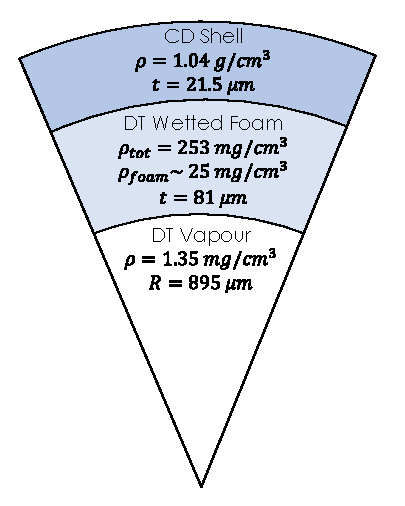
\includegraphics[width=.35\textwidth]{figures/LowCR/280Capsule.pdf}}
\subfigure b){\label{fig:280Hydro}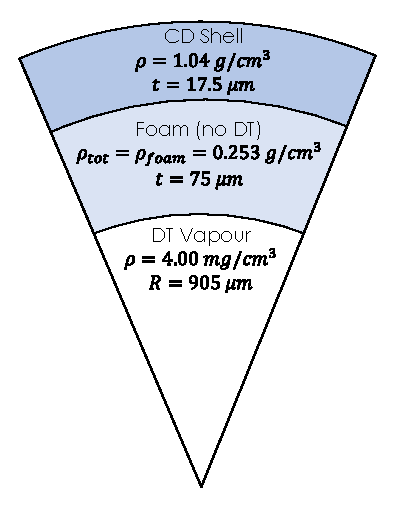
\includegraphics[width=.35\textwidth]{figures/LowCR/280Hydro.pdf}}
\caption{\label{fig:Hydroequivalent} a) The original 280 kJ wetted foam capsule. b) The 280 kJ hydroequivalent capsule. A higher foam density is used to compensate for the lack of DT, to give an equivalent layer density. The optimisation process if then reran, resulting in slightly different laser timings and layer thicknesses.}
\end{figure}

Hydro-equivalent versions of three different implosions have been developed, and are displayed (and compared to the original designs on which they are based) in Table \ref{tab:Hydroequivalent}. In each case, the new capsule was optimised according to the same optimisation procedure used in the previous chapter, maximising the gain of the implosion while satisfying the four criteria. In each case, this results in an implosion with much reduced yield and gain (due to the significantly reduced quantity of DT). However, the key hydrodynamic variables used to define the low instability regime - the convergence ratio, IFAR, and implosion velocity - are very similar to the original capsules, and continue to satisfy the low-instability criteria.

\begin{table}
\resizebox{\textwidth}{!}{%
\centering
\begin{tabular}{|c|c|c|c|c|c|c|}
\hline
Size multiplier &  \multicolumn{2}{c|}{0.35} & \multicolumn{2}{c|}{0.5} & \multicolumn{2}{c|}{0.65} \\ 
\hline
Hydroequivalent? & - & H.E. & - & H.E. & - & H.E.  \\
\hline
Laser energy (MJ) & 0.27 & 0.24 & 0.77 & 0.78 & 1.7 & 1.5 \\ 
Gain &  0.067 & 0.0094 & 0.19 & 0.016 & 0.75 & 0.023\\ 
Convergence ratio & 15.7 & 16.0 & 16.0 & 16.0 & 15.8 & 15.8 \\ 
IFAR & 27.5 & 28.4 & 29.7 & 29.4 & 25.1 & 29.3 \\ 
Implosion velocity (km/s) & 395.8 & 396.3 & 399.6 & 388.9 & 399.6 & 387.5\\ 
Max pulse power (TW) & 84.79 & 84.79 & 173.00 & 173.00 & 292.38 & 292.38\\ 
Pulse 2 switch on time (ns) & 2.20 & 2.70 & 2.60 & 2.50 & 3.60 & 3.70\\ 
Pulse 3 switch on time (ns) & 4.60 & 4.90 & 5.60 & 5.90 &7.80 & 7.80\\ 
Pulse 4 switch on time (ns) & 5.50 & 5.80 & 6.80 & 6.90 & 9.50 & 9.20 \\ 
Laser switch off time (ns) & 8.50 & 8.50 & 11.00 & 11.20 & 15.00 & 14.20 \\ 
Vapour/liquid boundary (\si[per-mode=symbol]{\milli\meter}) & 0.8950 & 0.9050 & 1.3050 & 1.3150 & 1.6705 & 1.7225\\ 
Liquid/CD boundary (\si[per-mode=symbol]{\milli\meter}) & 0.976 & 0.980 & 1.3950 & 1.3950 & 1.8200 & 1.8135\\ 
Outer radius (\si[per-mode=symbol]{\milli\meter}) & 0.9975 & 0.9975 & 1.4250 & 1.4250 & 1.8525 & 1.8525\\ 
Vapour density (\si[per-mode=symbol]{\milli\gram\per\centi\meter\cubed}) & 1.35 & 4.00 & 1.05 & 3.90 & 1.00 & 3.75\\
\hline
  \end{tabular}}
  \caption{Hydroequivalent implosions for three capsule size. The wetted foam implosion for each size has been included for comparison. All implosions use a four-pulse laser sequence. The hydroequivalent capsules have been optimised, resulting in slightly different values for the optimisation parameters and the laser energy, but the hydrodynamic parameters are broadly similar.}
  \label{tab:Hydroequivalent}
\end{table}

This provides a series of surrogate capsules, which could be used in room temperature experiments to validate this regime and verify the assumptions of low instability growth. These capsules could be shot, the amount of instability growth quantified, and their performance compared to the 1D simulations. If the instability growth is low and the agreement with the simulations good, then this would suggest that the four criteria used to define this regime are indeed sufficient to guarantee good agreement, and thus that the designs presented in the previous chapter would likely perform with similar agreement. 

\section{Alternative laser drivers} \label{sec:AlternativeDrivers}

A possible way to increase fusion performance is to increase the frequency of the laser driver. Higher frequency lasers have have a higher energy coupling with the plasma, which results in a greater ablation pressure for equivalent laser intensity. The higher frequency also has a higher critical density and can thus propagate further into the plasma, leading to increased laser absorption (since the light travels through more material) and a higher density blow-off \cite{Obenschain2020}. The lower laser wavelength also means that higher intensities are permitted before the onset of significant parametric instability growth \cite{Montgomery2016} (as highlighted by the $I \cdot \lambda^2$ criteria for the low-instability regime). 

The simulation platform described in the previous section is well-suited to an investigation of different laser drivers. The laser frequency can easily be changed in the Hyades input decks, and the same style of optimisation campaign can then be performed. The purpose of doing such is two-fold: the possible performance in the low-instability regime is further investigated, and the possible impact of increasing the laser driver can be investigated, quantified, and compared to the third-harmonic simulations in the previous section (all in a regime where reasonable agreement is expected between experiment and simulation). Two different laser drivers are considered in this section: a 193 \unit{\nano\meter} laser with a similar pulse profile to the previous simulations, and a novel `two-colour' laser driver.

\subsection{Background to possible IFE laser drivers}

Designs for IFE power plants have a number of requirements, including high laser efficiency, broadband laser operation, and (obviously) high gain. There are two main laser technologies that are seen as potentially satisfying these requirements; diode-pumped solid-state lasers (DPSSL) and electron-beam pumped excimer lasers, such as KrF or ArF \cite{Craxton2015}. 

The DPPSL fundamental wavelength is 1.05 \unit{\micro\meter}, which can be frequency tripled to 0.35 \unit{\micro\meter} - the same frequency used at the NIF, and thus that the previous simulations were performed for. The DPSSL technology is similar to that used at the NIF, where flash lamps are used to pump a solid state glass gain medium; but for DPSSL, the flashlights (which are inefficient, as they emit broadband light) are replaced with diode lasers which pump the medium at the appropriate frequency much more efficiently \footnote{the gain medium is not necessarily the same Nd:glass medium currently used at the NIF, but this is an option under consideration}. 

Excimer lasers are naturally higher frequency, with fundamental wavelengths of 0.258 \unit{\micro\meter} for KrF lasers and 0.193 \unit{\micro\meter} for ArF lasers. In excimer lasers, the gain medium is a gaseous mixture of a noble gas (Kr or Ar) and a halide (F). An electrical discharge is driven through the medium to excite it, leading to the formation of exciplex molecules - these emit UV radiation when they relax, and it is this relaxation which is used to provide the laser emission. There have been a number of excimer lasers developed (including Sprite/Titania at the CLF \cite{Divall1996}, Garpun at Lebedev Physical Institute \cite{Zvorykin2006}, and Nike at the NRL \cite{Obenschain1996}), but these have so far been limited to energies below 10 kJ. 

The `high average power laser' programme conducted between LANL and NRL investigated future laser drivers for IFE power-plants, and led to the development of high repetition rate lasers based on the two technologies \cite{Craxton2015}; the Electra KrF laser at the NRL (which could produce energies of up to 700 J and repetition rates of up to 5 Hz), and the Mercury DPSSL laser an LANL (which gave shots greater than 50J, with a repetition rate of up to 10 Hz \cite{Sethian2010}. Both lasers performed well, and this led to the conclusion that either technology could be viable for an IFE power plant and development of both approaches should be pursued.

Both approaches have their advantages. DPSSL lasers are likely more robust (as they are entirely solid-state), and the lower fundamental frequency is beneficial for preventing damage to laser optics \cite{Sethian2010}. However, excimer lasers have some strong advantages for direct-drive fusion performance. This includes the higher frequency (and thus greater laser absorbiton), but also a very smooth beam profile (desirable for direct-drive), good capability for focal zooming, and an inherently high bandwidth (significant for preventing parametric instability growth). These properties mean that simulations suggest that KrF or ArF lasers could be used to achieve higher gains for equivalent energies to DPSSL lasers. There is therefore a continuing interest in these technologies, as demonstrated by recently published simulations suggesting significant gains at low energies using ArF lasers for shock ignition \cite{Obenschain2020}.

\subsection{ArF lasers}

The optimisation procedure described in the previous chapter was repeated for a series of capsule sizes, but the laser frequency within the simulations was changed from the third-harmonic of Nd:glass to the 193~nm - the fundamental frequency of an ArF laser, and the same frequency used for the previously mentioned shock-ignition simulations \cite{Obenschain2020}. This can be easily achieved simply by changing the frequency in the HYADES input decks. In the low instability-regime outlined in the previous chapter, the maximum permitted laser power is set by a limit on $I \cdot \lambda^2$; increasing the frequency thus meant that the laser power could also be increased, while continuing to satisfy this criteria. All the laser powers were thus scaled accordingly. 

Other than the change to the laser frequency and the laser pulse powers, the simulation campaign was identical. The same capsule structure and four-pulse laser sequence was used, with the same seven optimisation parameters. This new campaign therefore is used to investigate the performance that could be achieved within the low-instability regime using an ArF laser. However, as the changes depend only on the frequency, this is used to demonstrate more broadly how moving to higher frequencies generally - be that from using a KrF laser (0.258 \unit{\micro\meter}), or using the fourth (0.263 \unit{\micro\meter}) or fifth (0.210 \unit{\micro\meter}) harmonic of Nd:glass - would influence the performance.

Three different capsule sizes were simulated and optimised by two summer students (Heath Martin and Rusko Ruskov) under my supervision. I provided the code required to do the simulation campaign, adjusted this to provide simulations at the new frequency with the new pulse powers, and then trained and supervised the two students as they performed the simulations. The tabulated results are displayed in \ref{tab:TwoColourTable}, and are plotted in \ref{fig:ArF and Two colour}.

\begin{figure}[ht]
\centering
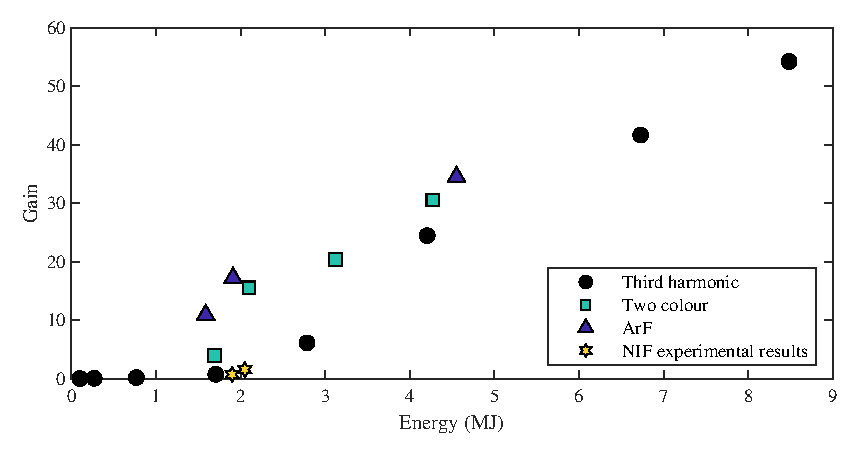
\includegraphics{figures/FurtherSims/ArFandTwoColour.eps}
\caption{A plot of the gain vs the laser energy for simulations using the three different laser drivers. The NIF 210808 experimental shot, and the recent NIF ignition shot, have been included for comparison.}
\label{fig:ArF and Two colour}
\end{figure}

\begin{table}
\resizebox{\textwidth}{!}{%
\centering
\begin{tabular}{|c|c|c|c|c|c|c|c|}
\hline
Laser driver   & \multicolumn{3}{c|}{ArF} & \multicolumn{4}{c|}{Two-colour} \\ 
\hline
Size multiplier & 0.45 & 0.5 & 0.65 & 0.5 & 0.65 & 0.75 & 0.85 \\
\hline
Total laser energy (MJ)  & 1.59 & 1.91 & 4.55 & 1.69 & 2.10 & 3.12 & 4.27\\ 
3rd harmonic energy (MJ) & - & - & - & 0.92 & 1.82 & 2.75 & 3.96 \\
ArF energy (MJ)  & 1.59 & 1.91 & 4.55 & 0.77 & 0.28 & 0.37 & 0.32\\
Gain & 10.9 & 17.3 & 34.5 & 4.0 & 15.5 & 20.4 & 30.5 \\ 
Convergence ratio  & 16.0 & 15.9 & 14.0 & 16.0 & 16.0 & 16.0 & 16.0\\ 
IFAR  & 11.3 & 10.5 & 8.5 & 16.1 & 20.4 & 23.8 & 23.4 \\ 
Implosion velocity (km/s)  & 390.7 & 398.9 & 360 & 391.1 & 399.9 & 396.4 & 391.6\\ 
Max 3rd harmonic power (TW)  & - & - & - & 173 & 292 & 389 & 500\\
Max ArF laser power (TW)  & 464 & 572 & 967 & 274 & 463 & 617 & 792\\ 
Pulse 2 switch on time (ns)  & 3.90 & 3.50 & 2.50 & 1.95 & 3.00 & 2.70 & 3.50\\ 
Pulse 3 switch on time (ns)  & 7.10 & 7.50 & 8.90 & 4.35 & 7.80 & 7.20 & 9.10\\ 
Pulse 4 switch on time (ns)  & 8.85 & 9.25 & 10.80 & 8.05 & 9.40 & 9.10 & 11.10\\ 
2nd laser switch on time (ns)& - & - & -  & 10.00 & 14.70 & 15.20 & 18.20 \\
Laser switch off time (ns)  & 11.95 & 12.25 & 15.10 & 12.80 & 15.30 & 15.80 & 18.60\\ 
Vapour/ice boundary (\si[per-mode=symbol]{\milli\meter})  & 1.072 & 1.210 & 1.435 & 1.230 & 1.645 & 1.933 & 2.210\\ 
Ice/CD boundary (\si[per-mode=symbol]{\milli\meter})  & 1.200 & 1.340 & 1.780 & 1.360 & 1.818 & 2.100 & 2.374\\ 
Outer radius (\si[per-mode=symbol]{\milli\meter}) & 1.2800 & 1.425 & 1.8525 & 1.425 & 1.8525 & 2.1375 & 2.4225 \\ 
Vapour density (\si[per-mode=symbol]{\milli\gram\per\centi\meter\cubed})& 1.00 & 1.03 & 0.60  & 1.02 & 1.05 & 1.00 & 1.01 \\
\hline
  \end{tabular}}
  \caption{Simulation parameters for the two-colour and high frequency implosions.}
  \label{tab:TwoColourTable}
\end{table}

It can be seen in Figure \ref{fig:ArF and Two colour} that the ArF implosions display a significant improvement in gain for a given energy compared to the previous third-harmonic simulations. A gain of 11 can be achieved for around 1.6 MJ of laser energy, which is an order of magnitude higher than is predicted using third-harmonic. This clearly displays the potential benefits of using a higher frequency laser driver. It should again be noted that this is in the low-instability regime, and thus it should be expected that instability growth would be minimal and 1D simulations should give a reasonable estimate of performance.

The physical properties of these implosions should also be commented on. For an ArF implosion the laser power is much higher compared to a third-harmonic implosion, but the limit on implosion velocity means that the implosion takes a similar amount of time. This means that the ArF implosion for a given capsule size has a much higher laser energy than an equivalently sized third-harmonic capsule (or alternatively, for the same energy the ArF implosion will use a smaller capsule). In terms of fusion performance, using a higher laser frequency has essentially shifted the ignition curve to lower energies; the capsule fuel mass has not changed, and so if the laser energy was allowed to increase indefinitely the yield would saturate at the same value. Rather, the ArF laser allows more favourable temperatures and densities to be achieved at a given energy, meaning that the onset of fusion reactions (and thus ignition) occur at lower energies. 

\subsection{Two-colour implosions}

Higher frequency lasers (whether excimer or higher harmonics of Nd:glass) are less technologically developed than third-harmonic Nd:glass lasers, and have not yet been demonstrated at such high energies. This makes the previous ArF results challenging to achieve in practice. As such, an alternative driver-scheme is proposed, where the higher frequency laser is used to supplement a third-harmonic driven implosion. This still requires much larger high frequency laser energies than are currently available, but it is a significant reduction compared to the previous simulations. The new scheme is a compromise solution, allowing some of the performance benefits of the higher frequency laser to be realised, without requiring such a large laser based on this novel technology. This concept will be referred to as a `two-colour' approach.

The laser scheme proposed is shown in figure \ref{fig:Two colour sequence}. A four-pulse third-harmonic sequence is applied, of the with the same pulse-profile as used in the previous simulation campaigns. Then, at a late stage in the implosion, a high-power short-duration pulse is applied at the higher ArF laser-frequency. While the four-pulse sequence was already at the maximum allowed power under the $I \cdot \lambda^2$ criteria, the lower wavelength of the final pulse means a higher power can be tolerated. The $I \cdot \lambda^2$ criteria is applied separately for the two lasers, given the large separation in wavelength between them (it has been demonstrated previously that using multiple frequencies leads to lower instability growth \cite{Follett2018}).

\begin{figure}[ht]
\centering
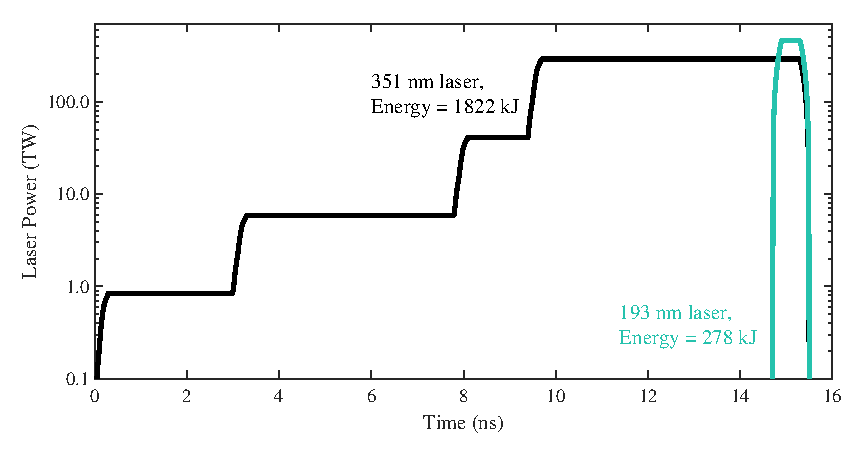
\includegraphics{figures/FurtherSims/TwoColourLaser.eps}
\caption{A log plot of laser power vs time for the 0.65 size two-colour implosion (which achieves a gain of 15.5). A four-pulse third harmonic laser is applied, which is supplemented by a single late pulse from an ArF laser. The ArF has a higher frequency, and thus a higher peak power can be used than for the third harmonic laser.}
\label{fig:Two colour sequence}
\end{figure}

As before, the four criteria for the low-instability regime continued to be applied. In particular, this meant that the implosion velocity was still unable to increase past 400 \unit{\kilo\meter\per\second} at any point in the implosion. This meant that heavier (thicker) shells were used which were accelerated to lower velocities by the third-harmonic laser, so that they continued to remain under the 400 \unit{\kilo\meter\per\second} limit once the high-frequency pulse has been applied. The addition of a late pulse made the optimisation more challenging, as it added an additional optimisation parameter (the switch on time of the final pulse). A  lower maximum ArF laser power was used for the late pulse than the maximum permitted under the $I \cdot \lambda^2$ constraint, or than was used for the ArF-frequency implosions; this appeared to be beneficial in preliminary simulations, but the more challenging optimisation procedure meant this parameter was not investigated further. 

Four two-colour implosions were optimised. I wrote the code to allow this new simulation campaign to be conducted/analysed and performed some preliminary simulations, with the main optimisation campaign then again performed by Heath Martin and Rusko Ruskov under my supervision. The results are displayed alongside those of the ArF simulations in \ref{tab:TwoColourTable}, and are plotted in \ref{fig:ArF and Two colour}.

It can be seen that, as expected, the results for the two-colour implosions consistently fit somewhere between those of the third-harmonic and ArF-frequency results. At 1.7 MJ, the two-colour sequence results in a gain of 4; lower than the gain of 11 achieved for a 1.6 MJ ArF sequence, but a significant improvement compared to the gain of 0.8 achieved using third-harmonic driver. Perhaps more significant is the gain of 15.5 achieved at 2.1 MJ, requiring only 280 kJ of the high-frequency laser. While still a significant increase over current energies for these lasers, this provides a clear demonstration of how this technique leads to significant increases in gain for much more moderate amounts of high-frequency laser energy; although it should be noted that this scheme would require a facility where the capsule can be irradiated uniformly using two different frequencies at the same time \footnote{This approach would therefore perhaps be more suited to higher harmonics of Nd:glass rather than an ArF laser, as then a single laser system could be used with the higher frequency provided by further frequency conversion on some of the beams}.

There are other features of this implosions that it is interesting to comment on. First, note the variation in the proportion of the total energy within the late pulse. This is likely a result of the difficulty in optimising these sequences, due to the additional optimisation parameter. These results are intended only as an initial investigation of this approach, but it appears that it may be possible to gain increased performance with further optimisation. Also, the low IFAR values of these implosions should also be noted, highlighting that this increased performance is achieved by accelerating thicker shells compared to the third-harmonic implosion. Some caution is required here when predicting the amount of Rayleigh-Taylor growth based on the IFAR value, due to the fact that the IFAR quoted corresponds to that measured when the capsule shell is at two thirds of the initial capsule radius. This is before the late-pulse is applied, and thus the IFAR value contains no information about the effect of this late pulse. Trends between the IFAR value and the amount of instability growth are based on experiments and theory which do not include the impact of this late pulse, and thus do not necessarily apply in the same way to the two-colour approach. However, low-instability growth is still predicted, due to three reasons: 1) the IFAR values are low even compared to the criteria of 30, allowing for some further compression of the shell; 2) the three additional criteria also serve to minimise instability growth; and 3) as the additional pulse is applied late, there is less time for any instabilities that it potentially seeds to grow. If this approach were to be pursued, these predictions should be tested with two-dimensional simulations.

\subsection{The burning plasma parameter for alternative laser drivers}

The burning plasma parameter for all of the implosions shown in Figure \ref{fig:ArF and Two colour} has been calculated\footnote{The terms were evaluated as follows: 1) the total work done $E^\mathrm{{tot}}_{\mathrm{PdV}}$ was evaluated as the sum of hotspot and shell kinetic and thermal energies, at the point during the deceleration of the shell where these two energies are equal. This corresponds to a period where the total energy of the capsule is constant, just prior to the onset of fusion reactions. 2) the deposited alpha energy over the full capsule was used rather than the hotspot for $E_\mathrm{\alpha}$, assuming that this absorbtion is dominated by the hotspot \cite{Christopherson2018}. These quantities were evaluated in this way to reduce the dependence of the calculated quantity on the exact position of the hotspot interface, so that it was more robust to issues with hotspot tracking.}, using Equation \ref{eqn:Qtot defn}. The ArF and two-colour implosions can all be seen to be well within the burning-plasma regime, with burning plasma parameters of around 10 and above. It can be seen that the 1.7 MJ third-harmonic implosion is the first third-harmonic result to achieve burning plasma.

\begin{figure}[ht]
\centering
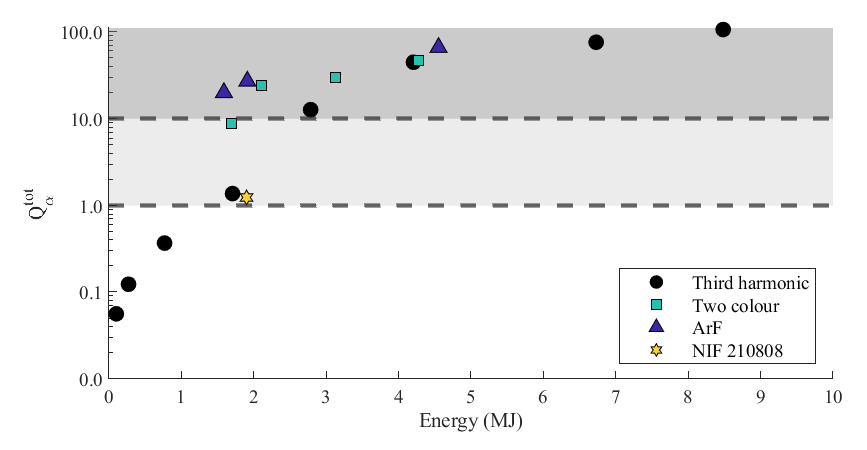
\includegraphics{figures/FurtherSims/QTwoColour.eps}
\caption{A log plot of the total capsule burning plasma parameter $Q^\mathrm{{tot}}_{\mathrm{\alpha}}$ vs laser energy for the optimised capsules using the three laser drivers. Values of $Q^\mathrm{{tot}}_{\mathrm{\alpha}} = 1$ and $Q^\mathrm{{tot}}_{\mathrm{\alpha}} = 10$ are indicated.}
\label{fig:TwoColourQ}
\end{figure}

NIF shot data for N210808 (the 1.3 MJ yield shot) has also been estimated and plotted on this graph, but this is very approximate and illustrative only. To do this, the reported shot data for 210808 \cite{Abu-Shawareb2022} was used to obtain the hotspot burning plasma parameter (this was plotted in \cite{Abu-Shawareb2022} and so could be estimated). The hotspot compression energy is assumed to be roughly half that of the total compression energy, giving an approximate total capsule burning plasma parameter that is half that of the reported hotspot burning plasma parameter \cite{Betti2015}. Insufficient data was available at the time of writing to plot this for the recent 3.5 MJ yield shot. As was noted with the gain of N210808, the burning plasma parameter suggests that the performance of this shot was close to (but slightly lower) than the simulated third-harmonic low-instability targets (although this is experimental data, compared to 1D simulated results which are likely an over-estimate).

\subsection{The zoomed focus technique}

Another potential benefit of these approaches are their compatibility with the `zoomed focus' technique. As the implosion occurs and the capsule is compressed, the critical surface of the capsule will move inwards (away from it's original position). However, the laser focus normally remains fixed at this original position. This smaller radius means that some light that previously would encounter the critical density surface will now miss it entirely. This results in reduced laser absorption. In addition, an increased amount of light travelling through the coronal plasma will contribute to increased cross-beam energy transfer, resulting in further decreased laser absorbtion and less uniform compression.

The `zoomed focus' or `zooming focus' technique sees the focus of the laser change during the course of the laser drive, allowing the laser spot size to be better matched to the imploding capsule \cite{Kehne2013, Eimerl2014}. While this is feasible but complex to achieve using conventional Nd:glass lasers \cite{Obenschain2015}, on excimer lasers (such as KrF or ArF) it is reasonably straight-forward to implement (due to differences in how the laser is smoothed) and it has been successfully demonstrated on the Nike KrF laser \cite{Kehne2013}. This would result in lower losses for an ArF setup compared to a third-harmonic driver (without such a technique implemented), and thus improvements to the fusion performance. The two-colour scheme is also a natural fit for such a technique; the high frequency laser can have a smaller focal spot than the third-harmonic laser, providing the `zoom' late in the implosion.

This effect is not included in the simulations presented here. In the 1D Hyades simulations, the laser provides perfect uniform and spherical illumination, and the laser is focused at the center of the target \footnote{It is possible in Hyades to use ray-tracing to simulate the impact of rays of light travelling at non-normal angles. However, it is not possible to include the effect of the finite spot-size, rather than an infinitesimally small focus. This is not sufficient to simulate the effect described here.} - meaning that the negative effects discussed above are not included. These simulations represent an ideal case, while the zoomed focus technique is an attempt to solve a non-ideal and practical problem. It should therefore be expected that implementing focal zooming (as could be done on ArF or two-colour implosions) would reduce a degradation mechanism not seen in the code, and thus give performance closer to that simulated than would be achieved without this technique.

\section{Auxiliary heating using relativistic electron beams} \label{sec:AuxiliaryHeating}

In Chapter \ref{ch-lowCR}, it was noted that the areal density of the hotspot for the 0.8 MJ capsule exceeded 0.3 \unit{\gram\per\centi\meter\cubed}. This is significant, as this is the areal density generally considered to be required for ignition to occur; and thus if the ion temperature could be increased in some way, it may be possible for this capsule to ignite and thus the gain to be significantly increased.

In this section, an auxiliary heating scheme is investigated which could potentially be used to increase the temperature of such capsules, thus improving the fusion performance. This is based on the scheme proposed and described by Ratan \textit{et al.} \cite{Ratan2017}. First, a brief description of the scheme will be provided - summarising how it was understood at the time that this work was performed, and (for completeness) developments since then. Then, how this was applied to the simulations from Chapter \ref{ch-lowCR} will be described, before the results are discussed. Finally, how such a scheme interacts with the higher gain capsules (achieved using alternative drivers) is investigated, along with alternative capsules optimised for areal density (rather than yield).

\subsection{Principles of the auxiliary heating scheme}

The scheme as described by by Ratan \textit{et al.} \cite{Ratan2017} works as follows. Two relativistic electron beams are produced and fired at a central hotspot implosion, such that they overlap within the hotspot. It was proposed that this was most suitable for low convergence ratio implosions, which have a large hotspot in which the beams could be overlapped. The electron beams lead to a bump-on-tail instability, which results in the growth of Langmuir waves, with energy transferred from the electron beam to these waves. These waves eventually undergo Landau damping, which smooths the distribution function and results in the transfer of the energy to the bulk electrons in the plasma and results in an increase in the electron temperature within the hotspot. Ion-electron collisions lead to an equilibration of the electron and ion temperatures, and so the ion temperature also increases. This process takes place over the order of a few picoseconds, which is very fast compared to the compression timescales of the capsule. In their investigation and description of this heating scheme, Ratan \textit{et al.} performed Vlasov simulations (which simulate the full distribution function of the electrons and ions) of overlapping electron beams within the plasma. This allowed them to estimate the growth rates of the different instabilities, and to predict (in fusion relevant plasma conditions) that energy is deposited from the electron beams into the plasma electrons with an efficiency of 18 \%.

How the electron beams are generated are not the focus of this work, but is a topic that has been explored  due to the application of such beams to fast ignition \cite{Tabak2005, Kemp2014}. Typically, it is expected that an ultra-high intensity short pulse laser would generate the electrons in the plasma through a range of potential interactions. These can include SRS and TPD in the low-density region of the plasma,  resonant absorption, vacuum heating\footnote{Also referred to as `Brunel' or `Not-so-resonant resonant absorption', this is a case of resonant absorption where electrons within the skin-depth of the critical density plasma are dragged out by the (rapidly-decaying) electric field associated with the EM wave, and then accelerated back into the high density region at high velocity a half-cycle later}, and $\vec{j} \times \vec{B}$ heating\footnote{This effect is important for high intensities, where the magnetic component of the EM wave cannot be neglected. If the wave travels normal to the critical density surface and the electric field causes electrons to oscillate in the direction of the E field, then the $\vec{v} \times \vec{B}$ component of the Lorentz force will also be normal to the surface, and electrons can be accelerated across the critical density surface}\cite{Wilks1997}.

The auxiliary heating scheme appears well suited to the designs presented in the previous chapter. It would be expected to drive a rapid increase in the ion temperature (as is required), leading to an increase in the fusion yield. The low convergence-ratio implosions also have the large hotspot that such a scheme requires. Since this work was performed, further research into this scheme has been performed which has improved the understanding of how it behaves \cite{Lee2023}; these new developments are discussed in Section \ref{sec:AuxHeatingDevlopments}.

\subsection{Simulating auxiliary heating in Hyades}

Simulating auxliary heating of ICF capsules is a challenging problem, due to the multi-scale nature of such a setup. Fluid such as Hyades can simulate the imploding capsule, but cannot simulate the auxiliary heating scheme itself as they do not include the physics necessary to describe the heating (it is not possible to generate Lagnmuir waves or to simulate Landau damping in such a code). Alternatively, particle-in-cell or Vlasov codes do include these effects, but cannot be feasibly ran over the nanosecond timescales and spatial scales required to simulate the ICF implosion. As such, approximations must be made.

In this work, Hyades is used to estimate the impact of the auxiliary heating, by estimating the effect that such a scheme would have on the electron energy. The Vlasov simulations performed by Ratan \textit{et al.} suggest that, for relevant conditions, the heating scheme would lead to an increase in the bulk plasma electron energy in the centre of the capsule. As such, Hyades simulations were performed where some amount of electron energy was added to the central zones (for convenience, this was done over those zones which initially contained the DT vapour at the start of the implosion), over a 7 picosecond window (corresponding to the timings from \cite{Ratan2017}) at a point just before the bang time of the implosion. The electron beams, Langmuir waves, and Landau damping are not simulated - but the estimated impact of such a scheme is. The effect this heating has on the fusion performance of the implosion is thus investigated.

The implementation in HYADES is demonstrated in Figure \ref{fig:EnergyDist}. In Figure \ref{fig:EnergyDist} (a), the thermal, kinetic, and total energy within a standard implosion (without auxiliary heating) over a 0.4 ns window around the bang time is seen. As the shell decelerates and the capsule stagnates, the kinetic energy decreases and the thermal energy increases accordingly. The total energy is initially constant, but a small amount of fusion reactions occur which leads to a small increase in energy (through alpha self-heating). In Figure \ref{fig:EnergyDist} (b), the same capsule is shown, but with 20 kJ of electron energy added in the central zones at the time represented by the dashed black line. This leads to a sudden and almost instantaneous jump in the thermal energy. this increase in the thermal energy and ion temperature leads to a significant increase in the amount of fusion reactions - as shown by the further increase in energy that occurs after the initial heating takes place.

\begin{figure}[ht]
\centering
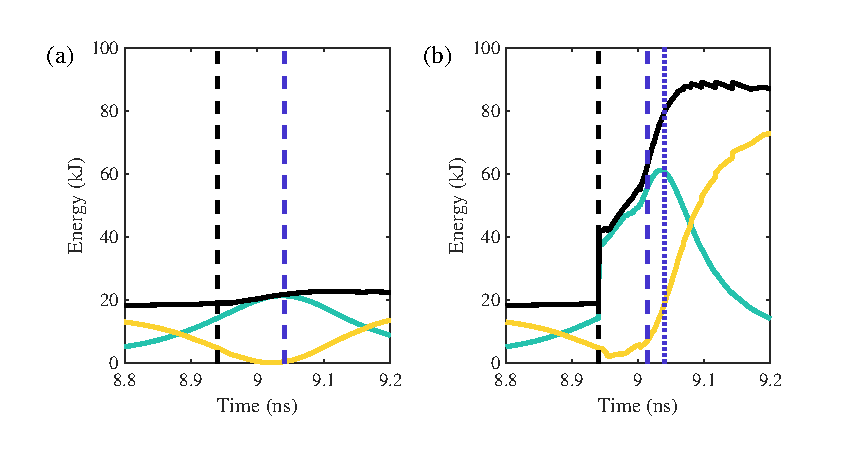
\includegraphics{figures/FurtherSims/EnergyDist.eps}
\caption{Plots showing the distribution of energy in a) an unheated capsule and b) a capsule where auxiliary heating is applied. The total energy is shown in black, with the kinetic energy in yellow and the thermal energy in teal. In both plots, the bang time is displayed by a dashed blue line, and the optimal time for auxiliary heating is a black dashed line. In b), the dotted blue line indicates the bang time for the unheated capsule (the dashed blue line in (a)), showing that the bang time occurs earlier in the implosion when heating is applied.}
\label{fig:EnergyDist}
\end{figure}

This demonstrates that adding electron energy in this way can indeed be used to improve the fusion performance of the capsule. In the following sections, this approach is applied to and investigated using four of the capsules developed in Chapter \ref{ch-lowCR}. The key data for these capsules has been summarised in Table  \ref{tab:Heating capsules} for convenience, where they are labelled capsules A-D. In the simulations discussed in this section, the implosion is unchanged from that reported in Table \ref{tab:ThirdHarmonic} apart from the addition of the electron energy. The capsule and laser parameters are not varied. Throughout this section, the laser in the simulation - the four-pulse third-harmonic profile optimised in the previous chapter - will be referred to as the `long-pulse' laser energy, to differentiate from the hypothetical `short-pulse' laser that would be used to generate the electron beam. The phrase `heating energy' will be used to describe the added electron energy; this is varied independently of the long-pulse laser, which always has the energy described in Table \ref{tab:ThirdHarmonic}.

\begin{table}
\centering
\begin{tabular}{|c|c|c|c|c|}
\hline
Capsule label &  A & B & C & D \\ 
\hline
Size multiplier & 0.25 & 0.35 & 05 & 0.65 \\
`Long-pulse' laser energy (kJ) & 101  & 270 & 768 & 1710 \\ 
Gain & 0.030 & 0.067 & 0.19 & 0.75\\ 
\hline
  \end{tabular}
  \caption{The four capsules (labelled A-D) for which the auxilliary heating is applied to. Only the key parameters are shown; refer to Table \ref{tab:ThirdHarmonic} for full simulation details}
  \label{tab:Heating capsules}
\end{table}

\subsection{Timing of electron energy deposition}

The timing at which the heating is applied to the implosion has a large impact on the increase in fusion performance. To investigate this, simulations were performed where 4 kJ of electron energy was added to each of the four implosions being simulated, at different times around the bang-time of the unheated implosions. The results are displayed in Figure \ref{fig:HeatingTiming}. The metric used here to evaluate performance is the relative yield amplitude, which is defined here as the yield of the capsule when the heating is applied compared to the yield without auxiliary heating \footnote{Note that this is different to it's conventional usage comparing the yield when alpha self-heating is/isn't included.}.

There is a clear peak in the yield amplification as a function of time for each capsule, indicating the optimal time for the heating to be applied. This optimal time is also that displayed in Figure \ref{fig:EnergyDist}, where it can be seen that it occurs just before the minimum in kinetic energy (as the shell stops moving inwards), and just before significant amounts of fusion reactions begin. This is unsurprising: adding the energy to the hotspot prior to this point would make it harder to compress and thus reduce the density, while adding it after significant fusion has occurred will mean that the burn wave has already started to propagate, and will mean that the added energy is smaller relative to the energy of the system. Further simulations repeating this with 20 kJ of injected energy observed the same behaviour and timings as Figure \ref{fig:HeatingTiming}, suggesting these optimal values are independent of the amount of energy added.

\begin{figure}[ht]
\centering
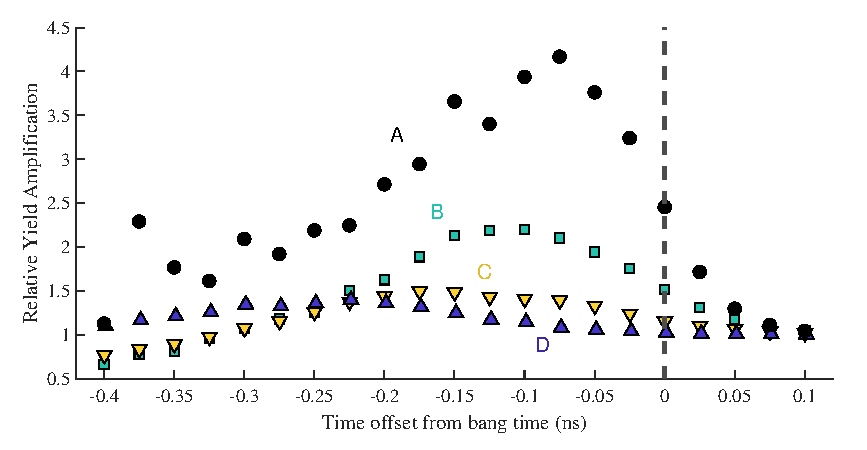
\includegraphics{figures/FurtherSims/HeatingTiming.eps}
\caption{Relative yield amplification for the capsules A-D as a function of time at which 4 kJ of electron energy is added. The capsule labels correspond to those in Table \ref{tab:Heating capsules}. The increased variation in capsule A compared to the others is likely due to the low gain of that capsule, as small changes in performance thus have a larger relative effect.}
\label{fig:HeatingTiming}
\end{figure}

\subsection{Magnitude of deposited electron energy}

Further simulations then investigated how the fusion performance varied as the amount of electron energy added was varied. The optimal time for energy deposition for each capsule from Figure \ref{fig:HeatingTiming} were identified, and the simulations then performed with between 3 to 60 kJ of electron energy deposited at this optimal time. The results can be seen in Figure \ref{fig:HeatingPower}. It can be seen that (as expected) adding more energy has a larger impact on the yield amplification, and even modest amounts of injected energy can have a significant effect. The relative yield amplification decreases as the capsule size increases; this is as expected, since 1) the larger capsules are higher energy, and thus the deposited electron energy is a smaller proportion of the capsule energy, and 2) the yield of the unheated capsule will be higher, and so a larger increase in yield is required for the same relative amplification.

\begin{figure}[ht]
\centering
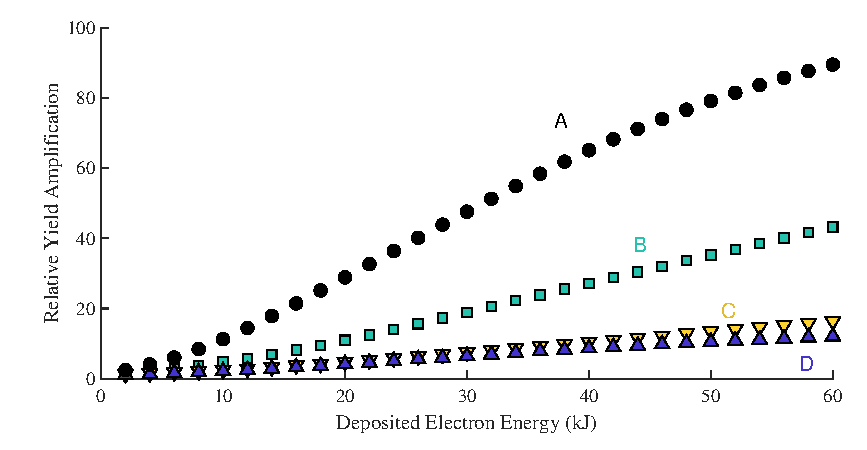
\includegraphics{figures/FurtherSims/HeatingPower.eps}
\caption{Relative yield amplification for capsules A-D as a function of the amount of deposited electron energy. The energy is injected at the optimal time for each capsule identified from Figure \ref{fig:HeatingTiming}.}
\label{fig:HeatingPower}
\end{figure}

The results are most notable for the smallest capsule (A), where 10 kJ of deposited energy gives over 10 times yield amplification, and 60 kJ amplified the yield by a factor greater than 80. Even for the largest capsule (D), 10 kJ of deposited energy is sufficient to double the yield, while 60 kJ amplifies the yield by over 12 times. This clearly shows the potential this scheme has for increasing capsule performance.

\subsection{The burning plasma parameter for heated capsules}

The (total capsule) burning plasma parameter $Q^\mathrm{{tot}}_{\mathrm{\alpha}}$ has been evaluated for the heated capsules A-D, and is displayed in Figure \ref{fig:HeatedQ}
as a function of the deposited energy \footnote{The terms were evaluated as follows: 1) the total work done $E^\mathrm{{tot}}_{\mathrm{PdV}}$ was evaluated as the sum of hotspot and shell kinetic and thermal energies just after the electron energy was added, such that the deposited energy is included in the calculation 2) the deposited alpha energy over the full capsule was used rather than the hotspot for $E_\mathrm{\alpha}$, assuming that this absorbtion is dominated by the hotspot \cite{Christopherson2018}}. These results again show the good level of performance achieved by all four capsules using auxiliary heating. While capsule D is already within the burning plasma regime, it can be seen that auxiliary heating enables both capusles B and C (which were initially sub-burning plasma) to enter it. The improvement in performance for all capsules is also clear from the improvement in $Q^\mathrm{{tot}}_{\mathrm{\alpha}}$ with heating; this is well demonstrated by capsule D which sees an improvement of almost a full order of magnitude. With the highest levels of heating it achieves a $Q^\mathrm{{tot}}_{\mathrm{\alpha}}$ approaching 10, suggesting that alpha self-heating adds almost ten times the energy to the capsule that the external compression.

\begin{figure}[ht]
\centering
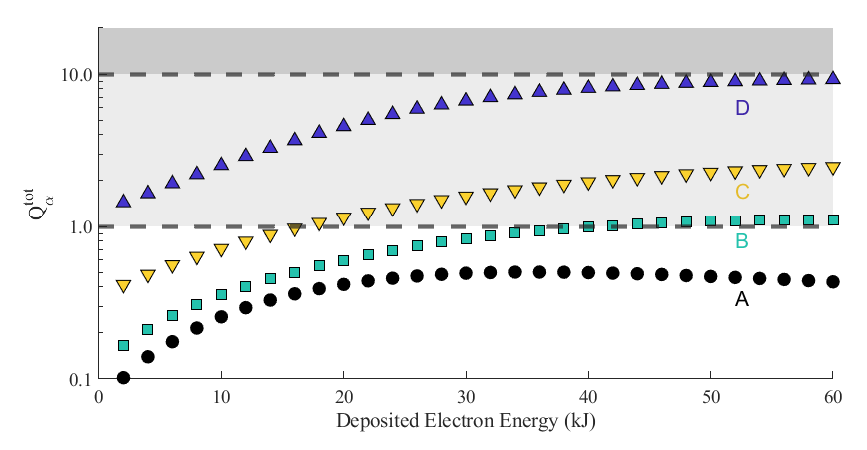
\includegraphics{figures/FurtherSims/QHeatingPlot.eps}
\caption{A log plot of the total capsule burning plasma parameter $Q^\mathrm{{tot}}_{\mathrm{\alpha}}$ vs deposited electron energy for the four capsules. Values of $Q^\mathrm{{tot}}_{\mathrm{\alpha}} = 1$ and $Q^\mathrm{{tot}}_{\mathrm{\alpha}} = 10$ are indicated.}
\label{fig:HeatedQ}
\end{figure}

\subsection{Estimating the gain of heated capsules}

Despite the challenges in calculating gain for these capsules, it is still the ultimate metric of interest for inertial fusion energy applications. Thus, the gain has been estimated using values for the relevant efficiencies from relevant literature. These efficiencies are not known to high accuracy, and thus these values are indicative only. There are two processes involved for which efficiencies must be estimated: 1) the deposition of energy into the plasma via the electron beams; and 2) the generation of the electron beams via short-pulse laser. The first of these conversion efficiencies can be taken from the Vlasov-Maxwell simulations reported by Ratan \textit{et al.} \cite{Ratan2017}, which found that the electron beams deposit electron energy with an efficiency of 18 \%.

Previous research on fast ignition has investigated electron-beam generation using short-pulse lasers, and have produced a range of estimates for the efficiencies with which such beams can be generated and transported (some examples are \cite{Ma2012, Kemp2014, Kemp2009}, and the review article \cite{Norreys2014}). For the estimates used here, two results are highlighted. The first is that of \cite{Strozzi2012}, who performed particle-in-cell simulations for an ignition scale plasma; they estimated an overall laser to electron power conversion efficiency of 52\%, which they then coupled to a hydrodynamic code for fast ignition simulations. The second is that of \cite{Tonge2009}, who also performed particle-in-cell simulations but found that as the electron beam passes through the weakly collisional background plasma a significant proportion of the energy is lost. They therefore calculated a lower efficiency of 15\% - although they also observed that this increased with both laser power, and the time for which the laser was applied. The maximum simulation time of 2.5 ps used in their work was lower than the 7 ps that the electron energy is deposited over in the Hyades simulations, iand so if this trend between deposition time and efficiency were to continue it is possible a higher effiency could be expected for this heating scheme.

In recognition of the range of values from different works, the value of 52 \% from \cite{Strozzi2012} and 15 \% from \cite{Tonge2009} have been used to provide two separate estimates of the gain. Each of these efficiencies have been combined with the 18 \% simulated coupling efficiency for electron beam energy deposition into the plasma to calculate an overall efficiency for the auxiliary heating process (capturing generation of the electron beams from short pulse laser, transport of these beams, and deposition into the plasma). The short-pulse laser energies required to cause the deposited electron energies in Figure \ref{fig:HeatingPower} were thus calculated; this was added to the `long-pulse' laser energy required for each implosion to calculate the total input energy, which was then used to calculate the gain. These two sets of estimates are displayed in Figure \ref{fig:HeatedGain}.

\begin{figure}[ht]
\centering
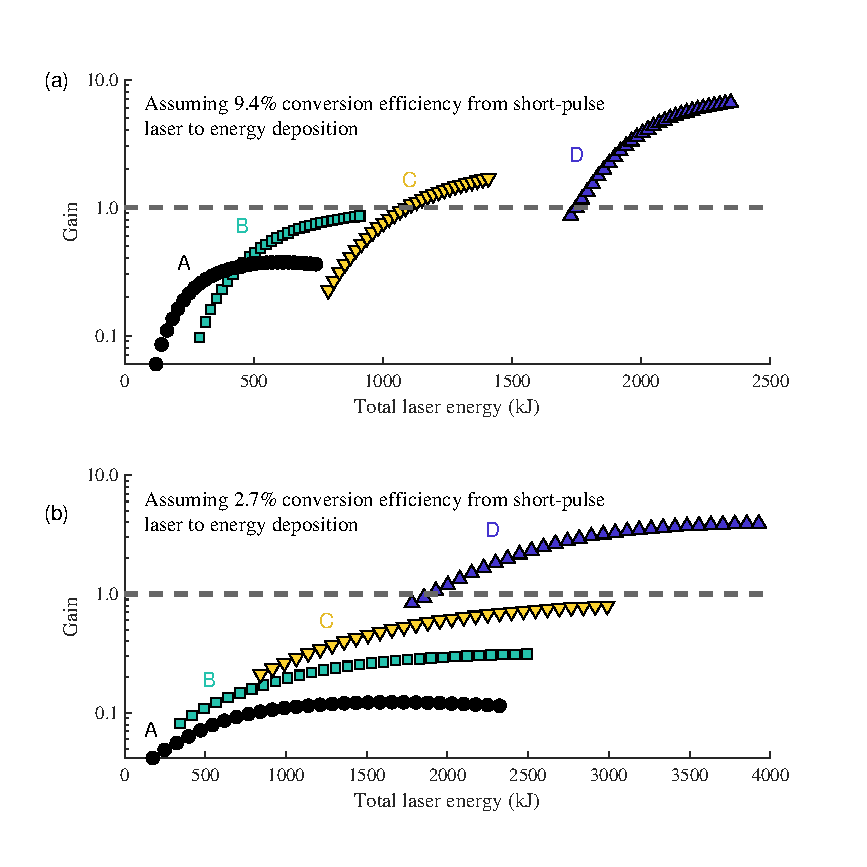
\includegraphics{figures/FurtherSims/HeatingGain.eps}
\caption{Estimated gain vs total input energy (including the `long-pulse' laser energy used to drive the implosion as reported in Table \ref{tab:Heating capsules}, and the estimated `short-pulse' laser energy required to generate the simulated amount of auxiliary heating. (a) and (b) use different estimates for the efficiency with which the heating can be generated, as indicated on the plots.}
\label{fig:HeatedGain}
\end{figure}

The general trends are the same in both figures; auxiliary heating causes an increase in gain, although this begins to saturate for larger amounts of heating energy. For the high efficiency case (a), higher gains can be achieved by using a smaller capsule with some auxiliary heating than through conventional hotspot ignition alone (as seen by the fact that lower energy capsules with a small amount of heating reach the same gains as the larger capsules for less total energy). This is unsurprising, as the 9.4 \% heating efficiency is higher than the roughly 6 \% efficiency for direct-drive laser compression \cite{Campbell2017, Goncharov2016}. For the lower efficiency case (b), direct-drive compression is higher efficiency, and so this is no longer observed. The saturation at large amounts of auxiliary heating is also not surprising; this is likely because both high density and high temperatures are required for high fusion yields, and at some point the density starts to become the limiting factor.

The results are obviously far more impressive for the high efficiency case, which predicts break-even for capsule C at around 1.1 MJ of total energy (using $\sim$ 350 kJ of short-pulse laser energy to deposit 32 kJ of electron energy into the hotspot), and gains of up to $\sim$ 3.5 for under 2 MJ of energy using capsule D. Given the observed trends, it appears likely that a capsule with size between B and C would achieve break-even for under 1 MJ of total energy. However, even in the low efficiency case, it is clear that auxiliary heating can still be a useful tool to improve the performance of a capsule, and capsule D can be seen to achieve break-even for under 2 MJ using this technique.

\subsection{Comparison with previous simulated and experimental results}

The results presented for capsules A-D can be compared to a range of previous results. Simulations were previously performed to estimate the impact such a scheme may have on indirectly-driven targets, which were presented in \cite{Norreys2021}. This was based on the NIF shot N160421, with a low convergence ratio and a drive energy of $\sim 800$ kJ. The greater efficiency of direct-drive implosions results in an approximately five-fold increase in the amount of energy deposited in the hotspot \cite{Campbell2017, Goncharov2016}, which means that such a capsule should be roughly equivalent to an implosion in this work with an energy of around 150 kJ. There are some minor differences between these works; the indirect-drive results demonstrate less dependence on the time at which the heating is applied, and a lower level of amplification than would be expected based on the results presented here (some differences should be expected due to the use of a different code, XRAGE, for the indirect drive simulations, and for the differences in the base implosions - with the indirect-drive implosion having significantly lower yield). Despite this the results are broadly similar between the two works, with similar trends observed in both the direct and indirect-drive simulations.

The fusion performance of capsule B is also comparable to that of NIF shots N190918, N191007, and N191110 (the capsules with record inertial fusion yields when this work was first performed \cite{Zylstra2021}), although these shots targeted higher convergence ratios over 25. These NIF shots produced neutron yields ranging from \num{0.75e16} to \num{2e16} (compared to \num{0.8e16} for capsule B without auxiliary heating) and fuel kinetic energies of $\sim$15~kJ (also similar to capsule B), for $\sim$1.9~MJ of indirect drive input energy. These shots led to predictions that laser energies of $\sim$3~MJ \cite{Zylstra2021} may have been required to achieve MJ-level yields (other predictions thought energies of up to $\sim$5~MJ may be required \cite{Zylstra2021, Cheng2021}). However, extrapolating the auxiliary heating results presented for capsule B to these implosions suggested that MJ-level yields could be achieved for a total of 2.3 MJ \footnote{This was estimated by taking the 56 kJ yield of N191110, and assuming based on implosion B in Figure \ref{fig:HeatingPower} that a yield amplification of twenty times could be achieved for 32 kJ of auxiliary heating, which would require less than 350 kJ of short-pulse laser energy assuming a conversion efficiency of 9.6 \%.}. This highlights how such a heating scheme could potentially be used to improve the performance of real NIF shots. These results could also be extrapolated for the 1.3 MJ yield shot N210808. This has a yield between those of capsules C and D; applying a similar extrapolation suggests that this yield could be doubled for only 10 kJ of deposited energy. These are illustrative examples only, but serve to demonstrate how this technique could be applicable more widely than just for the low-instability shots discussed here.

\subsection{Auxiliary heating of high gain capsules}
Auxiliary heating was also later applied to three of the alternative laser drivers implosions. The main purpose of this was to see the effect of auxiliary heating on high gain capsules; auxiliary heating helps the capsule to achieve ignition without adding more fuel, and thus it is likely that for better performing capsules the increase in performance would be more moderate. It also allowed the combination of these technologies to be assessed. These simulations were performed by summer students Tat Li and Eugene Kim, under my supervision.

Three capsules were used: the 0.5 and 0.65 size two-colour implosions, and the 0.5 size ArF implosion \footnote{These simulations were performed a year after the capsules were first optimised, and used the updated HYADES version 01.12.05 compared to version 01.12.03 for the original simulations. Rerunning the unheated input decks using this new version resulted in a slightly increased yield. This explains why the gain at low heating levels in Figure \ref{fig:TwoColourAux} is still higher than that reported in Table \ref{tab:Heating two colour capsules}.}.  These capsules are labelled E-G in Table \ref{tab:Heating two colour capsules}. The auxiliary heating was simulated exactly as described in the previous sections, and the optimal timing for the heating was identified as outlined previously, before the amount of deposited energy was varied. The results are shown in Figure \ref{fig:TwoColourAux}.

\begin{table}
\centering
\begin{tabular}{|c|c|c|c|}
\hline
Capsule label &  E & F & G  \\ 
\hline
Laser driver & \multicolumn{2}{c|}{Two-colour} & ArF \\ 
\hline
Size multiplier & 0.5 & 0.65 & 0.5 \\
\hline
`Long-pulse' laser energy (MJ) & 1.69  & 2.10 & 1.91 \\ 
Gain & 4.0 & 15.5 & 17.3 \\ 
\hline
  \end{tabular}
  \caption{The three high gain implosions (labelled E-G) for which the auxilliary heating is applied to. Full details can be found in Table \ref{tab:TwoColourTable}.}
  \label{tab:Heating two colour capsules}
\end{table}

\begin{figure}[ht]
\centering
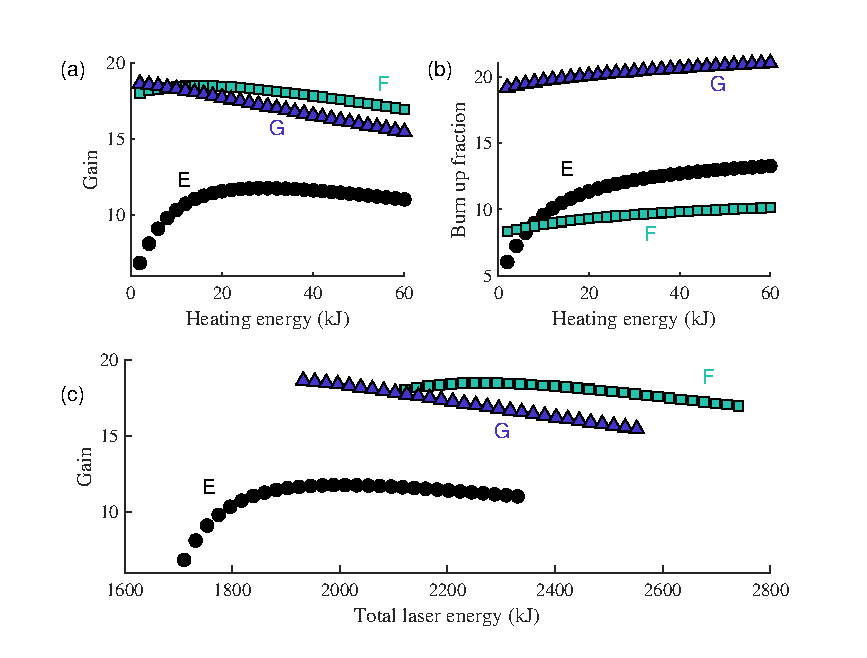
\includegraphics{figures/FurtherSims/TwoColourAux.eps}
\caption{Auxiliary heating for two two-colour implosions (E and F) and one ArF implosion (G). In (a), the estimated gain (assuming a 9.4 \% heating efficiency) is plotted as a function of the heating energy. In (b), the burn-up fraction of the three implosions versus heating energy is displayed. (c) shows the estimated gain, as a function of the total estimated input energy.}
\label{fig:TwoColourAux}
\end{figure}

As expected, it was found that for higher gain capsules, the auxiliary heating is much less beneficial. The 0.5 size capsule has the lowest base gain, and it can be seen that adding electron energy allows the gain to increase by a moderate amount, but after this it actually begins to decrease. This corresponds to a scenario where the additional fusion reactions generated by the increase in energy no longer compensate for the additional cost. This is not unexpected - this capsule has already achieved the conditions necessary for a large amount of fusion reactions to occur, and thus the amount of electron energy deposited (as a fraction of the hotspot energy) is much less significant than for the previous capsules.

As the yield of the unheated implosion further increases, this effect becomes even more dramatic. The 0.65 size two-colour capsule sees an even smaller fractional increase in performance, and less electron energy can be added before the gain begins to decrease. For the ArF capsule, adding electron energy offers no benefit and the gain decreases from the start. This is despite the unheated gain being very similar to that for the 0.65 size two-colour capsule. The reason for this is that the ArF capsule is smaller (the energy is the same due to the higher laser power), and has a much higher burn up fraction (as shown in Figure \ref{fig:TwoColourAux} (b)). The unheated ArF capsule is therefore further along it's ignition curve - it is already igniting very well, and is close to the maximum possible yield for this capsule. The two-colour capsule is larger, with more fuel and a higher saturation gain, and thus the performance can be further increased compared to the ArF capsule.

\subsection{Optimisation and heating of high areal-density capsules}
The implosions A-D (and the high gain capsules) are each implosions that were originally optimised for high gain, in the absence of auxiliary heating. However, it may be that if the conventional implosion and the auxiliary heating were considered together, there may be alternative implosions that would return a higher gain once the heating is applied.

This would add significant complexity to the optimisation, which makes it infeasible to explore without further development. However, it is possible to predict the form of such an implosion. Auxiliary heating allows the temperature of the capsule to be significantly increased, but the areal density is unchanged. As such, it was suggested that if an implosion could be developed with a higher areal density (at the expense of a lower temperature and yield), then once auxiliary heating is applied to increase the ion temperature the resulting yield/gain may be higher than if a capsule optimised for yield was heated.

To explore this, a further two optimisations were performed. This followed the exact procedure as before, but the implosions were optimised to produce a capsule with the maximum possible areal density (i.e. the areal density of DT within both hotspot and shell), rather than yield. I again produced the changes to the code necessary to enable this, and then supervised a summer student, Tat Li, in performing the optimisation. The resulting `optimal areal density' implosions are included in Table \ref{tab:Optimal Areal Density}, along with the corresponding `high gain' version. Auxilliary heating was then applied, first identifying the optimal timing for the capsules, and then varying the deposited energy. The resulting gains (assuming the optimistic 9.4\% conversion efficiency for the heating) is then displayed in Figure \ref{fig:OptimisedRhoR}.


\begin{table}
\centering
\begin{tabular}{|c|c|c|c|c|c|c|}
\hline
Laser driver & \multicolumn{2}{c|}{Third harmonic} & \multicolumn{2}{c|}{ArF} \\ 
\hline
Size multiplier & \multicolumn{2}{c|}{0.5} & \multicolumn{2}{c|}{0.5} \\ 
\hline
Optimised for & Gain & $\rho R$ & Gain & $\rho R$  \\
\hline
Laser energy (MJ)  & 0.77 & 0.80 & 1.91 & 2.16 \\ 
Gain (original) &  0.19 & - & 17.3 & -\\ 
Gain (at time of work) &  0.19 & 0.12 & 18.7 & 24.7\\ 
Areal Density (\unit{\gram\per\centi\meter\squared}) & 0.71 & 0.76 & 1.04 & 1.30\\
Convergence ratio  & 16.0 & 15.9 & 15.9 & 15.9 \\ 
IFAR  & 29.7 & 23.2 & 10.5 & 9.0 \\ 
Implosion velocity (km/s)  & 399.6 & 358.1 & 398.9 & 361.9\\ 
Pulse 2 switch on time (ns)  & 2.60 & 3.60 & 3.50 & 4.20\\ 
Pulse 3 switch on time (ns) & 5.60 & 6.80 & 7.50 & 9.20\\ 
Pulse 4 switch on time (ns)  & 6.80 & 8.20 & 9.25 & 11.00 \\ 
Laser switch off time (ns)  & 11.00 & 12.60 & 12.25 & 14.40 \\ 
Vapour/liquid boundary (\si[per-mode=symbol]{\milli\meter})  & 1.305 & 1.290 & 1.210 & 1.150\\ 
Liquid/CD boundary (\si[per-mode=symbol]{\milli\meter})  & 1.3950 & 1.390 & 1.340 & 1.340\\ 
Outer radius (\si[per-mode=symbol]{\milli\meter})  & 1.425 & 1.425 & 1.425 & 1.425\\ 
Vapour density (\si[per-mode=symbol]{\milli\gram\per\centi\meter\cubed})  & 1.050 & 1.200 & 1.030 & 1.405\\
\hline
  \end{tabular}
  \caption{Newly optimized `optimal areal density' implosion simulation parameters, for the 0.5 size third-harmonic and ArF implosions. The data for the original `optimal gain' implosions have been included for comparison.}
  \label{tab:Optimal Areal Density}
\end{table}

\begin{figure}[ht]
\centering
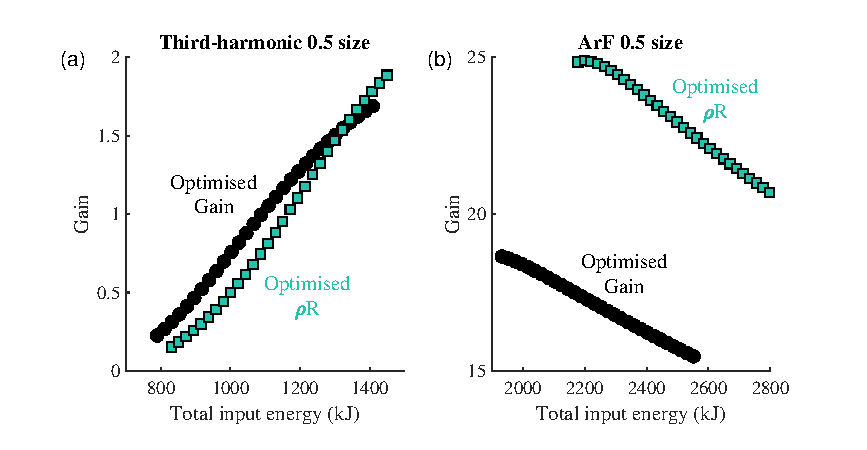
\includegraphics{figures/FurtherSims/OptimisedRhoR.eps}
\caption{Estimated gain vs total input energy for the 0.5 sized capsules optimised for gain (black) and areal density (teal), for a third-harmonic (a) and ArF (b) laser driver.}
\label{fig:OptimisedRhoR}
\end{figure}

The gain for the smaller of the two capsules, seen in Figure \ref{fig:OptimisedRhoR}, behaved as predicted. It can be seen that at low amounts of heating energy the `optimal gain' capsule outperforms the `optimal areal density' version, as expected. However, as the heating energy is increased further, the `optimal areal density' capsule begins to perform better, producing a higher gain that the `optimal gain capsule'. The `optimal gain' capsule begins to saturate earlier - this makes sense, since it has a lower areal density and a higher temperature, and so the temperature stops being the limiting factor much earlier than for the `optimal areal density' version.

A number of factors mean that the data in Figure \ref{fig:OptimisedRhoR} is more complicated to analyse. Firstly, the optimisation procedure in this case gave an `optimal areal density' capsule at a higher laser drive than the `optimal gain' capsule (recall that this is the optimal capsule for a given radius - and not necessarily a given drive energy). The higher laser drive meant that the capsule gain was also higher, hindering useful comparison between the two capsules \footnote{This also indicates, as explained earlier, that the optimisation is not exhaustive - as there is clearly a design for this capsule radius with a higher gain than that initially optimised.}. As seen in Figure \ref{fig:OptimisedRhoR} (b), the gain is therefore higher for all amounts of deposited energy. Secondly, the much higher gain of this capsule means that the auxiliary heating in both cases does not lead to significant increases in gain, as discussed in SECTION. However, qualitative differences are still visible - although increases in gain are not seen, it is clear that `optimal areal density' capsule is still improved more by the heating (despite the higher gain and laser energy), as indicated by the fact that the gain is relatively constant at low energies as opposed to decreasing (as seen for the `optimal gain' capsule). This is confirmed by the relative yield amplification, which shows a greater relative increase for the `optimal areal density' capsule at low energies.

\subsection{Limitations and suggested future direction}

As stated at the start, the simulations presented here are an initial investigation of the effects of such a heating scheme. They do not simulate the scheme itself, and thus high accuracy should not be expected. However, they indicate a promising level of performance, and suggest that further investigation of this heating process in more detail could be useful. This includes simulations of the full heating process using Vlasov-Maxwell and particle-in-cell codes, along with multi-scale modelling. These are directions that are under further investigation within our group.

Another limitation of this work is the lack of accuracy to which the efficiencies for the generation and transport of the electron beams are known. These efficiencies are vital for accurate estimates of the implosion gain, and so should be determined if such a scheme is to be pursued.

A final potential limitation of this approach are the high short-pulse laser energies required. These are significantly higher than the short-pulse energies available at current facilities, and are similar to those necessary for fast-ignition schemes \cite{Strozzi2012}. Again, this an an initial investigation of this approach, which is focussed on whether such a scheme may be worthwhile than the practical aspects of achieving it. However, recent developments such as plasma beam combiners \cite{Kirkwood2018,Kirkwood2018a} may offer a route through which short-pulse laser energies could be increased in the future to the levels required \cite{KirkwoodPersonalComm}. Plasma beam combiners utilise non-linear scattering interactions within plasma-based optical components to produce a single laser output from multiple input beams, achieving a much higher intensity than is possible with conventional optics. It is hoped that continued development of this approach, and of short-pulse laser technology more generally, may enable the energies required for such a scheme.

\subsection{Subsequent developments of the auxiliary heating technique} \label{sec:AuxHeatingDevlopments}
Since this work was performed, there have been further developments in understanding this technique which affect how it would be applied; these are described in \cite{Lee2023}. This is not my work (it was performed by Jordan Lee, Rusko Ruskov, and Heath Martin) - but it was performed following the promising results shown here, and is mentioned for completeness and improved understanding of the technique.

In the previous discussions, the heating scheme was assumed to require two overlapping electron beams. This was the setup proposed in \cite{Ratan2017}; the highest growth rates for the instabilities was seen at the overlap of these beams, and it was expected that this would therefore be where the most significant heating occurred. Having two beams in this way allowed for control over where the energy would be deposited. However, further research instead discovered that there is no benefit to using two beams - the heating growth quickly saturates, and thus two beams provides no benefit over one. The heating occurs along the beam according to the plasma conditions, and thus the position of the energy deposition cannot be controlled in this way.

Simulations of an electron beam incident on the capsule around the bang-time found that the vast majority of the energy is deposited at the edge of the hotspot. The electron beam passes through the cold, dense shell with very little absorption, but is absorbed effectively as soon as it reaches the high temperature hotspot. This is different to the simulations here, where the energy deposition was assumed to be uniform over the central region in the simulation. However, updated versions of these HYADES simulations (performed by Jordan Lee) accounted for this, instead depositing the electron energy in a thin shell (of appropriate thickness) around the hotspot. It was found that these actually slightly improved the performance\footnote{It is suggested that this is because the material at the edge of the hotspot is likely slightly higher density but colder - and thus the heating has more of an effect}. This assumes that the heating is spherical, whereas in fact this would only occur in the direction of the beam - 2D simulations are required to investigate this in further detail.

\section{Conclusions}
This chapter expanded upon the results of the previous chapter in a variety of different ways. Firstly, two potential limitations of the previous work were explored. The impact of the EOS used to describe the wetted-foam layer was investigated through simulations in the alternative 1D code HELIOS, where a PropacEOS `mixed-EOS' table could be used which included the CH foam. This investigation was limited (due to the need to use an alternative code, and the lack of alpha-heating in HELIOS), but suggested that using a more accurate EOS for the foam layer could potentially decrease performance by around 30\%, which is comparable to other results published in the literature. Secondly, surrogate `hydrodynamic equivalent' implosions were optimised for a number of capsules, and displayed equivalent hydrodynamic performance to the main implosions. This provides a way that the results of the previous chapter (and the low-instability nature of the regime) could be explored in room-temperature experiments.

The impact of alternative laser drivers on implosions in this regime were then explored. It was demonstrated that switching from a third-harmonic Nd:glass laser to a higher frequency (ArF in this work) could lead to substantial increases in fusion performance at a given energy. A `two-colour' laser sequence was also proposed, which would allow some of the performance benefits of higher frequency laser energies to be obtained, while allowing the bulk of the energy to be provided by the more mature Nd:glass technology.

Finally, the effect of auxiliary heating on a number of these implosions was simulated. It was found that such a technique could potentially be used to significantly improve the fusion performance of a range of capsules. The increase on gain was also estimated to be significant, but this is highly dependent on how efficiently electron beams can be generated and their energy deposited into the hotspot. Further simulation identified that the impact is significantly decreased as the yield of the unheated implosion increases, suggesting that auxiliary heating is more useful for helping sub-ignition capsules to ignite rather than amplifying the gain of already well-performing capsules. 






%%\begin{savequote}[8cm]
%Alles Gescheite ist schon gedacht worden.\\
%Man muss nur versuchen, es noch einmal zu denken.

%All intelligent thoughts have already been thought;\\
%what is necessary is only to try to think them again.
 % \qauthor{--- Johann Wolfgang von Goethe \cite{von_goethe_wilhelm_1829}}
%\end{savequote}

\chapter{\label{ch:2D}Two-dimensional simulations of the low instability regime}

\minitoc



%\begin{savequote}[8cm]
%Alles Gescheite ist schon gedacht worden.\\
%Man muss nur versuchen, es noch einmal zu denken.

%All intelligent thoughts have already been thought;\\
%what is necessary is only to try to think them again.
 % \qauthor{--- Johann Wolfgang von Goethe \cite{von_goethe_wilhelm_1829}}
%\end{savequote}

\chapter{\label{ch-experiment}Measuring the TMPTA principal Hugoniot}

\minitoc

\section{Introduction}

Foams are interesting to study for a variety of reasons. Their relevance to this thesis is obvious: their role in the wetted-foam capsules discussed extensively in previous chapters, and in the hydrodynamic-equivalent capsules proposed in SECTION. However, they also have potential application in laser beam smoothing and imprint mitigation \cite{Depierreux2009, Hu2018} (where the foam is used to spread energy from an incoming laser beam laterally, reducing the imprint issues associated with direct-drive), adiabat shaping \cite{Craxton2015, Bodner1998, Collins2005} (where the adiabat can be shaped so that the outside of the shell is higher adiabat - and thus less susceptible to instability growth - while the inner fuel is kept on a lower adiabat and can thus be better compressed), increasing absorption of Nd-laser light \cite{Skupsky2004} (as the laser can propogate further into the material, due to regions where it is underdense, compared to a uniform material), and increasing conversion from laser light into X-rays \cite{Shang2016}. As a result foams are of significant research interest; with particular interest on the topics of homogenisation (how the inhomogenous foam transitions over time to a homogeneous plasma) and the impact of micro-structure on foam compression \cite{Hazak1998, Cipriani2021, Cipriani2018a, Colvin2013}.

An interesting question surrounding foams is how best to describe them in equation of state models. The inhomogeneity of the material could potentially have significant effect - with the voids within the structure requiring energy to close, costing energy, before more regular compression can begin. This process is not well modelled - and indeed, it is common to see foam described in simulations as a low-density version of the homogeneous material upon which they are based (as was done in the simulations in earlier sections). However, previous experiments have shown that such an approach can be inaccurate \cite{Nicolai2012}. Inaccuracies in the equation of state have significant implications for simulations which aim to describe such foams, making this a potential barrier for wetted-foam implosions.

This problem motivated us to propose and perform an experiment to investigate the equation of state - through principal Hugoniot measurements - of fusion-relevant TMPTA plastic foam, using the VULCAN kJ-class Nd:glass laser at the UKRI-STFC Rutherford Appleton Laboratory. This experiment is described in this chapter. First, the basic concept of the experiment will be discussed, along with the initial experiment setup and plan. The experiment itself will then be covered, along with changes from this initial plan. The analysis, results and interpretation will be considered in the subsequent chapter.

This experiment was a large international collaboration between a number of institutions, but the work I present was largely performed by me. I will highlight where work I present was performed by someone else. I prepared the initial proposal for the experiment, which my supervisor submitted as PI. I then performed most of the preparation work before the experiment (which was supported by simulation work by some of my collaborators). I attended the experiment for the full run, and was the scientific lead throughout, supported by a large number of collaborators. At the start of the experiment these collaborators also served as `target-area operator', before I also took on this role for the final three weeks. Finally, I performed the large majority of the analysis - again supported with data and some simulation work by my collaborators.

\section{Experiment overview and diagnostics}

A mutli-layer target, containing a layer of TMPTA plastic foam at an initial density of 260~\unit{\milli\gram\per\centi\meter\cubed}, was shocked via irradiation from the Vulcan laser. The target was a sandwich design consisting of four layers: an $\sim$~40~\si[per-mode=symbol]{\micro\meter} CH ablator, followed by an $\sim$~3~\si[per-mode=symbol]{\micro\meter} gold layer, an $\sim$~40~\si[per-mode=symbol]{\micro\meter} $\alpha$-quartz reference layer, and then finally the $\sim$~40~\si[per-mode=symbol]{\micro\meter} TMPTA foam. A schematic of this target can be seen in Figure \ref{fig:target}. VULCAN was used to irradiate the CH layer - material was ablated, and this generated a strong shock which propagated through the target. The gold layer prevented pre-heating of the quartz/foam, by absorbing any x-rays generated in the coronal plasma.

\begin{figure}
\centering
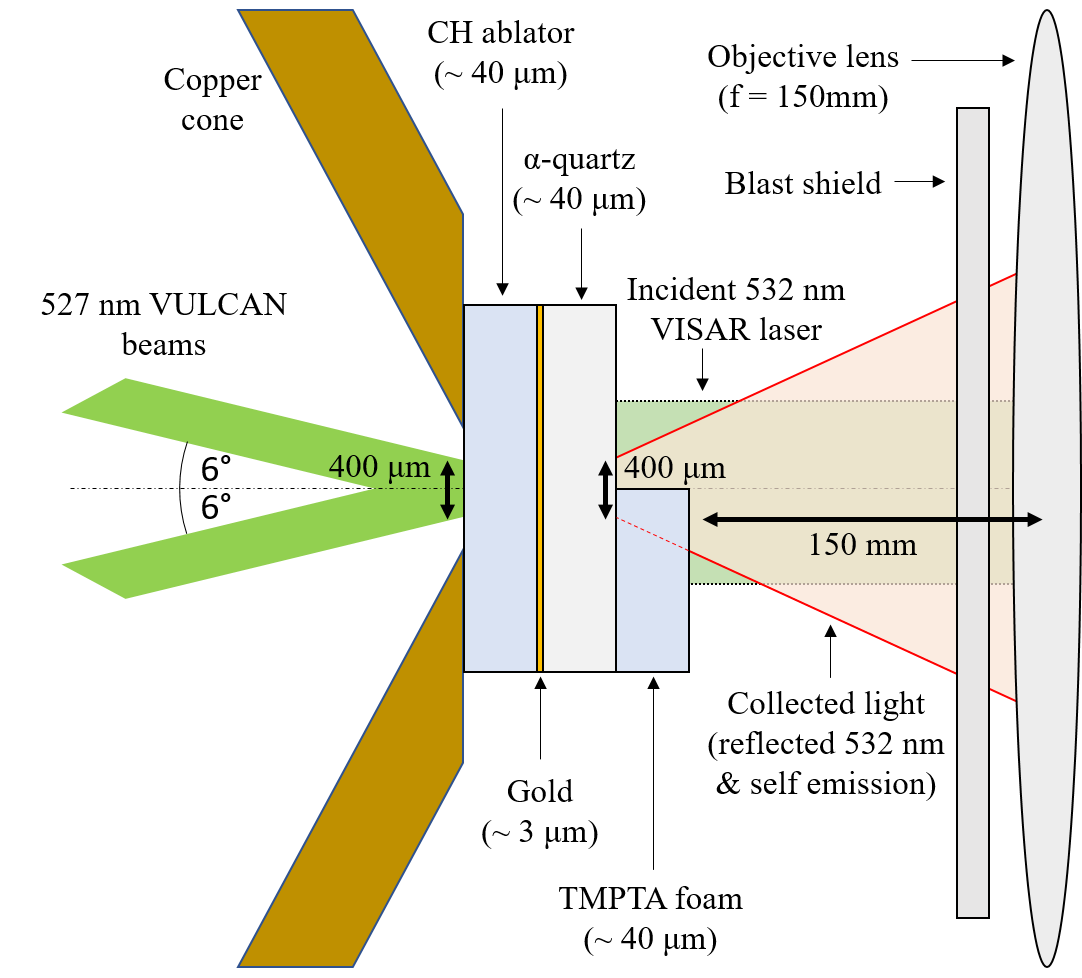
\includegraphics[width=0.45\textwidth]{figures/Experiment/TargetSchematic.png}% Here is how to import EPS art
\caption{\label{fig:target} Simple schematic showing the target and objective lens (top view, not to scale)}
\end{figure}

The shock was roughly uniform over a $\sim$~400~\unit{\micro\meter} diameter. To generate this, the six main VULCAN beams were overlapped spatially to produce a `top-hat' beam with a $\sim$~400~\unit{\micro\meter} diameter. The pulse power profile was also a `top-hat', with a rise and fall time of $\sim$~200~\unit{\pico\second}. 

The target had a step in the rear side, so that the TMPTA foam only covered half of the quartz surface in the $\sim$~400~\unit{\micro\meter} shocked region. This meant that both quartz and foam were visible to the diagnostics, and is similar to targets used in previous experiments to investigate other materials \cite{Falk2014a, Falk2020}. The shock velocity in both layers was measured using VISAR, which was driven using a probe laser reflected off the rear surface of the target. The shock temperature of both layers was determined using streaked optical pyrometry (SOP).

The quartz layer in this experiment was used as a reference material for an impedance matching calculation. The shock velocity in both the quartz and the foam were measured in each shot and used to determine the foam shock state; the theory behind this process is described in Sections \ref{IMTheory} and \ref{IMTheoryMeasurements}. This defines a shock  state on the foam Hugoniot per shot. By performing a series of shots at different laser powers (and thus intensities), a the Hugoniot curve could therefore be populated over a range of pressures.

\subsection{The VULCAN laser}

The VULCAN laser is a user-facility based at the UKRI-STFC Rutherford Appleton Laboratory's Central Laser Facility. It is a 2.6 kJ Nd:glass laser with a fundamental frequency of 1053 \unit{\nano\meter}, with 8 beamlines (6 long-pulse, and 2 short-pulse) and two experimental areas providing different operational modes. At Target Area West, the 6 long-pulse beams are available alongside 2-short pulse beams. The long-pulse beams can each deliver energies ranging from 300 \unit{\joule} to 50 \unit{\joule}, dependent on pulse lengths ranging from 0.5 \unit{\nano\second} to 10 \unit{\nano\second}. These beams can be converted to second harmonic using KDP crystals (with some conversion losses) \cite{Ross1981}. The short-pulse beams can either both deliver 1 \unit{\pico\second} pulses, or offer a mixture of 1 \unit{\pico\second} and 10 1 \unit{\pico\second} pulses, with an intensity up to mid $10^{19}$ \unit{\watt\per\centi\meter\squared}. At Target Area Petawatt, a single short-pulse petawatt beam can provide intensities of up to $10^{21}$ \unit{\watt\per\centi\meter\squared} at shorter pulse times of $500$ \unit{\femto\second} (or lower powers and intensities for pulse times up to tens of \unit{\pico\second}), alongside a long-pulse beam line with the aforementioned properties.

Each beamline begins with a `seed' pulse, which is amplified to produce the main beam \cite{Ross1981}. For the long-pulse beams this seed is relatively high energy, and thus the preamplfication stage consists of a single rod amplifier \cite{Springate2010}. The pulse the enters the main amplification stage, where it is amplified by a series of further glass amplifiers. After each round of amplification, the beam diameter is increased; this reduces the intensity, which keeps it below the damage threshold of the laser glass. Rod amplifiers are used up to a diameter of 45 \unit{\milli\meter}, above which more efficient disk amplifiers are used \cite{Springate2010}. 

Producing short-pulse high intensity beams can be challenging, as above a threshold damage intensity the beam can no longer be amplified using conventional glass amplifiers. This issue was resolved by the invention of chirped pulse amplification (CPA) \cite{Strickland1985}. In this process, a relatively low power `seed' pulse with a short pulse length is `stretched' temporally, by chirping the beam so that the frequencies become separated out. The longer pulse i can be amplified up to the damage threshold of conventional optics, before being compressed back to the original pulse length by reversing the chirp. This short-pulse now has an intensity significantly higher than that of the damage threshold.

On VULCAN, CPA is used for the short-pulse beams. A short seed pulse is produced, stretched temporally, and then pre-amplified by a few rod amplifiers. The beam then undergoes the main amplification process described for the long-pulse beams, before being compressed in the target chamber.

For the Petawatt beamline, a 120 \unit{\femto\second} initial pulse is stretched to 4.2 \unit{\nano\second} \cite{Hernandez-Gomez2006} and preamplified through mulitple rounds of optical parametric chirped pulse amplification (OPCPA) \cite{Musgrave2015}. OPCPA is a variation on CPA, where optical parametric amplification (OPA) is used - a process through which a powerful `pump' laser is used to amplify a weaker signal laser \cite{Ross1997}. OPA is used rather than glass amplifiers due to the gain narrowing effect; the eventual short pulse duration imposes a stringent minimum bandwidth requirement, and gain narrowing in glass amplifiers prevents this from being achieved \cite{Danson2004}. Using optical parametric amplification initially and then optimising the subsequent glass amplifiers to maximise this bandwidth enables this requirement to be satisfied. The pulse then undergoes amplification as described for the other beams.

Finally, each beam is delivered to the target area. The short-pulse beams are compressed, reversing the effect of the chirp and resulting in a shorter and thus higher power laser pulse. All the beams also have a large diameter by this stage, and are focused down to a small spot to give a high intensity on target.

This experiment was conducted in Target Area West, and used only the six long-pulse beams. These were frequency doubled to second harmonic, and focused using custom phase plates into a single `top-hat' style laser spot with a diameter of 400 \unit{\micro\meter}. The same pulse was requested from each beam, coincident in time, to produce a single flat-topped laser pulse. This pulse time was varied throughout the experiment between 2 \unit{\nano\second} and 9 \unit{\nano\second}; this resulted in a range of pulse energies and intensities, thus driving shocks of a range of different strengths.

\subsection{VISAR}

VISAR (an acronym for `velocity interferometer system for any reflector') is a velocity interferometry technique, which allows the velocity of a moving surface to be detected \cite{Barker2000, Barker1972}. A probe laser is reflected from the surface to be measured, and the reflected light is passed into the interferometer (or `the VISAR'). The interferometer produces a fringe pattern, from which the velocity of the surface can be calculated. In this experiment, VISAR is used in this way to determine the shock velocity of the quartz (while also being used to identify breakout times, allowing the average foam shock velocity to be calculated).

A simple scehmatic of a VISAR is shown in Figure \ref{fig:VISAR_Schematic}. The interferometer consists of two legs. Leg `B' contains an etalon, and this serves to delay light passing through this leg by a time $\tau$ compared to the light passing through leg `A'. The effect of this is two photons which arrive at the recombination beamsplitter from the two different legs will have entered the VISAR unit at different times, separated by this delay time $\tau$. This means that the photons will also have reflected from the surface at different times, and as therefore have encountered the surface at different positions (since it is moving). The distance travelled by the two photons will therefore differ based on the surface velocity - this information, through the phase difference, is encoded in the resulting interference pattern.

\begin{figure}
\centering
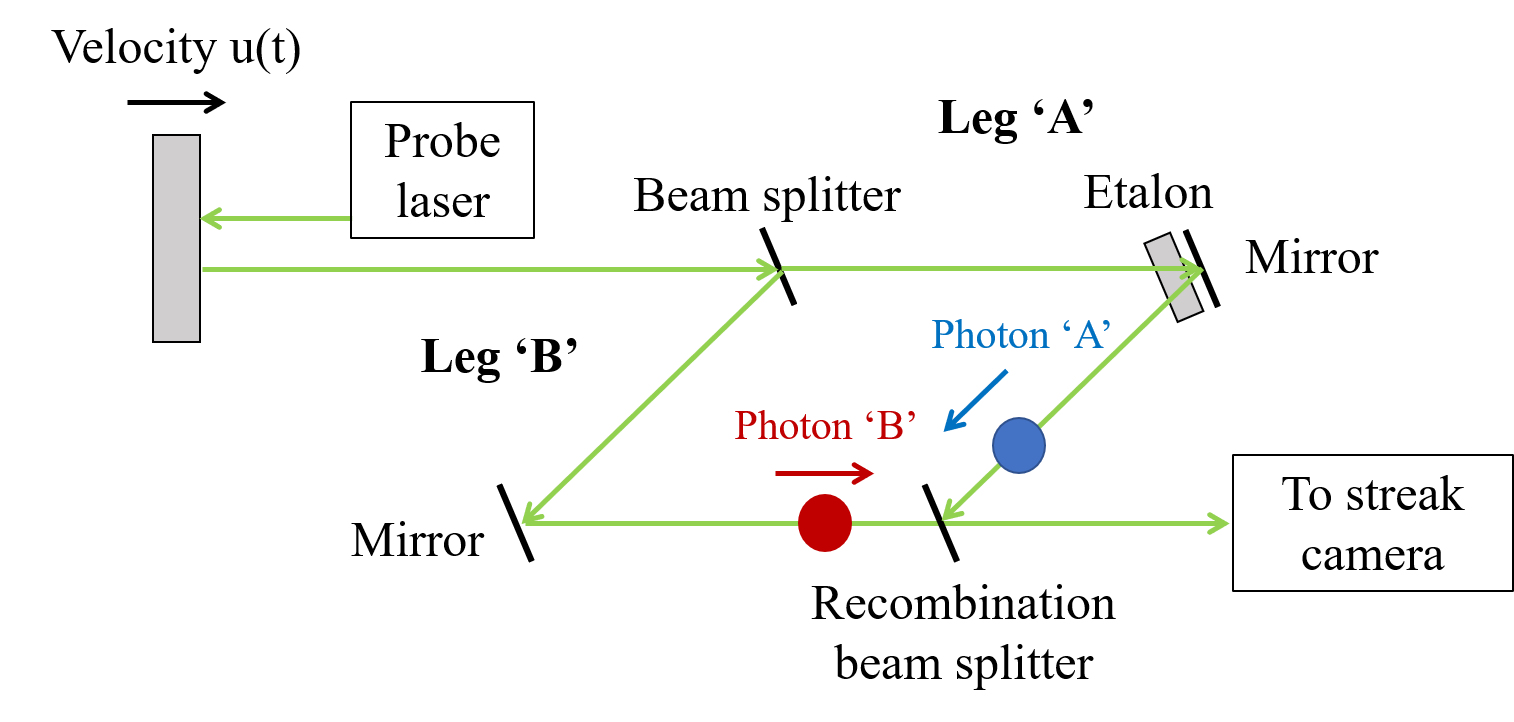
\includegraphics[width=0.6\textwidth]{figures/Experiment/VISARSchematic.png}% Here is how to import EPS art
\caption{\label{fig:VISAR_Schematic} Simple schematic of a VISAR. Photon `A' and photon 'B' travel down different legs to arrive at the recombination beam splitter at the same time and interfere with one another. These photons entered the VISAR (i.e. reached the first beam splitter) at different times; as the delay leg (leg 'A') takes an extra time $\tau$ to transit compared to leg 'B', photon 'A' must therefore have entered the VISAR a time $\tau$ earlier than photon 'B'.}
\end{figure}

Numerous mathematical descriptions of the VISAR exist. The one presented here is a simple explanation which considers the signal from the point of view of interferometry, as suggested originally in \cite{Barker1968} (and conceptually similar to the explanation given in \cite{Barker2000}). This derivation neglects the doppler shift caused by the moving mirror, and instead simply considers the change in the mirror position to derive the correct result. Alternative derivations derive the same behaviour through the doppler effect\footnote{The most simple form of this derivation is that presented in \cite{Barker1968}. Using the same variables defined in the main equation, the moving mirror introduces a doppler shift in the light of $\Delta \lambda (t) = - \frac{2 \lambda}{c} u(t)$. The length of the delay leg can be written in terms of multiples of the laser wavelength, $N \lambda = c \tau$. Differentiating this gives $\Delta N(t) = - \frac{c}{\lambda^2}\Delta \lambda (t)$. Substituting in the expression for $\Delta \lambda (t)$ then gives $u(t) = \frac{\lambda}{2\tau} \Delta N(t)$. The interference pattern is based on the difference in path length between the two legs, and thus the fringe shift is proportional to $\Delta N$ - leading to the same equation for the VPF as the main derivation.}, but these often ignore the phase difference due to the movement of the surface. Derivations based on this approach can be found in numerous sources \cite{Barker1968, Barker1972, Barker2000, Hammel2018}. More complete derivations (such as those by Clifton \cite{Goosman1975a}, Goosman \cite{Goosman1975} and Bennett \cite{Bennett2016}) reconcile these two approaches.

Consider photons A and B in Figure \ref{fig:VISAR_Schematic}, which travel down the VISAR legs A and B respectively. Both arrive at the recombination beamsplitter at the same time. Photon A travelled down the delay leg, and thus took a time $\tau$ longer than photon B to travel through the VISAR - for them to arrive at the same time, it must therefore have entered the interferometer a time $\tau$ earlier.

Before entering the VISAR, both photons travel from the probe laser to the reflective surface, and then from the surface to the VISAR. For the photon `A', travelling at the earlier time, this distance can be denoted as $D$. If the surface is moving, then photon B travelling at a different time will encounter the surface in a slightly different position. It therefore travels a distance $D+2d$, where $d$ accounts for this small change (it is multiplied by two, accounting for the fact that the photon will travel this distance both to and from the surface). This distance d is given by \begin{equation} d = \int_{t_1}^{t_2} u(t') \cdot dt' = \int_{t_1}^{t_1 + \tau} u(t') \cdot dt',\end{equation} where $u(t')$ is the surface velocity as a function of time $t'$, $t_1$ is the earlier time at which photon A encounters the surface, and $t_2$ is the time at which photon B encounters it. The approximation $t_2 = t_1 + \tau$ has been made, which neglects the time taken for the photon to cover the distance d; this is reasonable, since the distance $d$ is very small and thus this time is typically much smaller than the time delay $\tau$ introduced by the etalon. The time $t_1 = t - T$ can be linked explicitly to the time at which the measurement is made at the streak camera $t$ by considering the time $T$ it takes the photon A to reach the streak camera; the distance $d = d(t)$ is therefore itself clearly shown to be a function of time.

The two photons therefore have a total path difference (when they interfere at the recombination beamsplitter) of $ \Delta x = 2d + \epsilon $, where $\epsilon$ is the (constant) additional path length introduced by the etalon. This leads to a phase difference of \begin{equation} \Delta\phi = k (2d + \epsilon),\end{equation} where $k = 2\pi / \lambda$ is the wave vector. Following the standard theory for interference between two waves \cite{Hecht2017}, the resulting intensity is given by  \begin{equation}I = I_1 + I_1 + 2\sqrt{I_1 I_2} \cos{\Delta \phi},\end{equation} where $I_1$ and $I_2$ are the intensity of the two waves in the different interferometer legs. As these are of equal intensity, $I_0 = 2 I_1 = 2 I_2$ can be declared and this equation simplified to \begin{equation} I = I_0 (1 + \cos{\Delta \phi}) = I_0 (1 + \cos{k (2d + \epsilon)}).\end{equation}

In this form, the intensity profile does not depend on spatial position (assuming that velocity is constant across the surface), and thus the interference `pattern' would be constant spatially. In order to produce spatial fringes, the recombination beamsplitter is rotated slightly to introduce a small linear phase ramp. This gives an intensity of \begin{equation} \label{eqn:VISAR eqn}I \propto  I_0 [1 + \cos(k (2d + \epsilon + x\sin(\theta) ))],\end{equation} where $x$ is the spatial position and $\theta$ is the (constant) angle of the beamsplitter, adding spatial dependence and resulting in a repeating pattern of fringes.

At this point, it is useful to consider two illustrative cases. First, consider the situation when the surface is stationary, or moving at a constant velocity $u_1$. In this case the distance $d$ will be given by $d = \tau u$, and will be constant. Equation \ref{eqn:VISAR eqn} will then feature no time dependence, and the fringe pattern will be constant as a function of time, described by 
\begin{equation} I(t_1) \propto I_0 [1 + \cos(\phi_1)] =  I_0 [1 + \cos(k (2\tau u_1 + \epsilon + x\sin(\theta)))].\end{equation}
Now, consider that the velocity of the surface changes to a new constant velocity $u_2$. This will result in a new fringe pattern described by \begin{equation}I(t_2) \propto I_0 [1 + \cos(\phi_2)] =  I_0 [1 + \cos(k (2\tau u_2 + \epsilon + x\sin(\theta)))] = I_0 [1 = cos(\phi_1 + 2k\tau \Delta u)] \end{equation}
representing a small fringe shift from the original pattern based on the difference in the two velocities $\Delta u = u_2 - u_1$. It is clear that there will be a single fringe shift when $2k\tau \Delta u = 2 m \pi$, where $m$ is any integer. The 'velocity per fringe', or VPF, is the velocity change that accompanies a full fringe shift, and is therefore defined as \begin{equation} VPF = \frac{\lambda}{2\tau}. \end{equation}

A small correction is applied to this equation, \begin{equation} VPF = \frac{\lambda}{2\tau (1 + \delta)}, \end{equation} to account for dispersion within the etalon $\delta$ \cite{Barker1974}. Further specific corrections can also be required depending on the precise experimental target configuration \cite{Barker1970, Celliers2004}.

This shift in fringes thus allows the velocity of the surface to calculated. The VISAR begins recording when the surface is stationary, and as the surface moves the total fringe shift is recorded. The VPF can then be used to calculate the surface velocity based on this fringe shift, allowing the velocity profile of the surface as a function of time to be determined. Analysis of VISAR data follows this principle, and a description of how this is performed in practice is provided in Appendix \ref{appdx: VISAR analysis}.

%\subsection{Old VISAR explanation}

%VISAR (or `Velocity Interferometer System For Any Reflector') is a velocity interferometry technique which allows the velocity of a moving surface to be measured. A probe laser is reflected from the measurement surface, and the reflected light captured and passed into the interferometer (often referred to as `the VISAR'). The resulting fringe pattern contains information about velocity changes at the surface. In this experiment, the VISAR is used to determine the shock velocity of both the quartz and the foam.

%A simple schematic of a VISAR is shown in figure. The reflected probe laser is split by a beamsplitter, and passes down two seperate legs, before being interfered at a recombination beamsplitter. An etalon is used so that the delay leg has a longer optical path, and thus a longer transmission time. This means that the photons interfering at the beamsplitter from the two different legs entered the interferometer at differnt times, and thus the interference is thus between the laser, and the laser released a short time previously.

%The effect of this is that the photons being interfered at the recombination beamsplitter entered the 

%This has a significant effect. As there is a difference in the transmission time through the two legs ($\tau$), two photons which arrive at the recombination beamsplitter entered the interferometer at different times. This means the interference is between the laser light, and the laser light a time $\tau$ previously. The resulting interference pattern thus is due to the changes in the phase of the beam over time. 

%These phase changes arise from the movement of the target, which is what enables velocity measurements using this technique. Consider the photon that arrives first. To reach the interferometer, the photon travelled from the laser to the measurement surface, and then back to the interferometer - a distance $D$. Now consider the second photon. In the time $\tau$, the surface has moved by a distance $d = \tau u$, where u is the average velocity of the surface over that time. The total distance the second photon travels is therefore $D+2d$ - a longer distance, which results in a phase shift (the factor 2 accounts for the fact that this distance must be covered twice. (A more rigorous analysis would include the fact that it would take some time to cover the distance d, but this is essentially negligible given that the the photon travels at the speed of light).

%The total path difference of the two beams at the recombination beamsplitter is therefore $\tau u + \delta$, where $\delta$ is the additional path length introduce by the delay etalon. This path difference results in a phase difference of $\phi = k (\tau u + \delta)$, where $k = 2\pi / \lambda$ is the wave vector. The resulting interference pattern varies according to the phase as $cos(\phi) = cos(k (\tau u + \delta)$. As described, and assuming no spatial variation in the reflector, the phase difference would be spatially constant. In order to produce a fringe pattern, the beamsplitter is rotated slightly to introduce a small linear phase ramp in the spatial position $x$, so that $\phi = k (\tau u + \delta + xsin\theta)$. This means that the image is now a fringe pattern.

%Consider the case where the surface is stationary or moving at a constant velocity, so that $u$ is a constant. In this case, the phase difference $\phi$ between the two signals is constant as a function of time, and thus the interference pattern is stationary - resulting in a static fringe pattern. However, consider the case where the surface velocity is changing, and thus $u$ varies. In this case, the phase will change by $k\tau \Delta u$, and thus the fringe pattern will also move. The pattern will repeat when $k\tau \Delta u = n\pi$ where n is an integer, and thus a full fringe change will occur when the change in velocity $\Delta u = \lambda /2 \tau$.

%In this way, the velocity of the surface can be determined. The experiment is begun with a stationary surface, and as the velocity changes the fringe pattern will be altered. The fringe shift F(t) is recorded, and can be converted into a velocity using this `Velocity per fringe', or VPF. This enables dynamic measurement of velocity vs time. The VPF needs an additional correction to account for dispersion, which leads to an actual VPF of \hl{equation}

\subsubsection{Etalon selection}

The etalon used in the VISAR determines the delay time $\tau$, and thus determines the VPF of the system. Using a thicker etalon results in a larger time delay and a lower velocity per fringe, giving increased velocity resolution. The value of $\tau$ also determines the time resoltion of the system; if a velocity change occurs in a time less than $\tau$, it will be recorded as a sudden discontinuity in the phase pattern.

Accurate determination of the velocity requires the fringe shift F(t) to be known. A discontinuity in the phase pattern prevents F(t) from being known with certainty, as the fringe pattern repeats if velocity increases by the VPF. A fractional phase shift could therefore correspond to a number of possible velocities, each seperated by integer multiples of the VPF. However, the ambiguity in velocity this causes can be resolved by introducing a second VISAR, using a different etalon. As long as the VPFs of the two etalons are not integer multiples, and sudden change in velocity will cause different fractional phase shifts on the two VISAR systems. Only one velocity will be compatible with the fractional phase jump measured on the two systems, and thus the velocity of the surface can be unambiguously calculated.

\subsubsection{VISAR design and operation}

A labelled diagram of the VISAR used in this experiment is displayed in Figure \ref{fig:Dan_VISAR}. This VISAR was developed and designed by Daniel Eakins. While the main components are the Mach-Zehnder interferometer, the overall device contains a series of optics to aid with alignment.

\begin{figure}
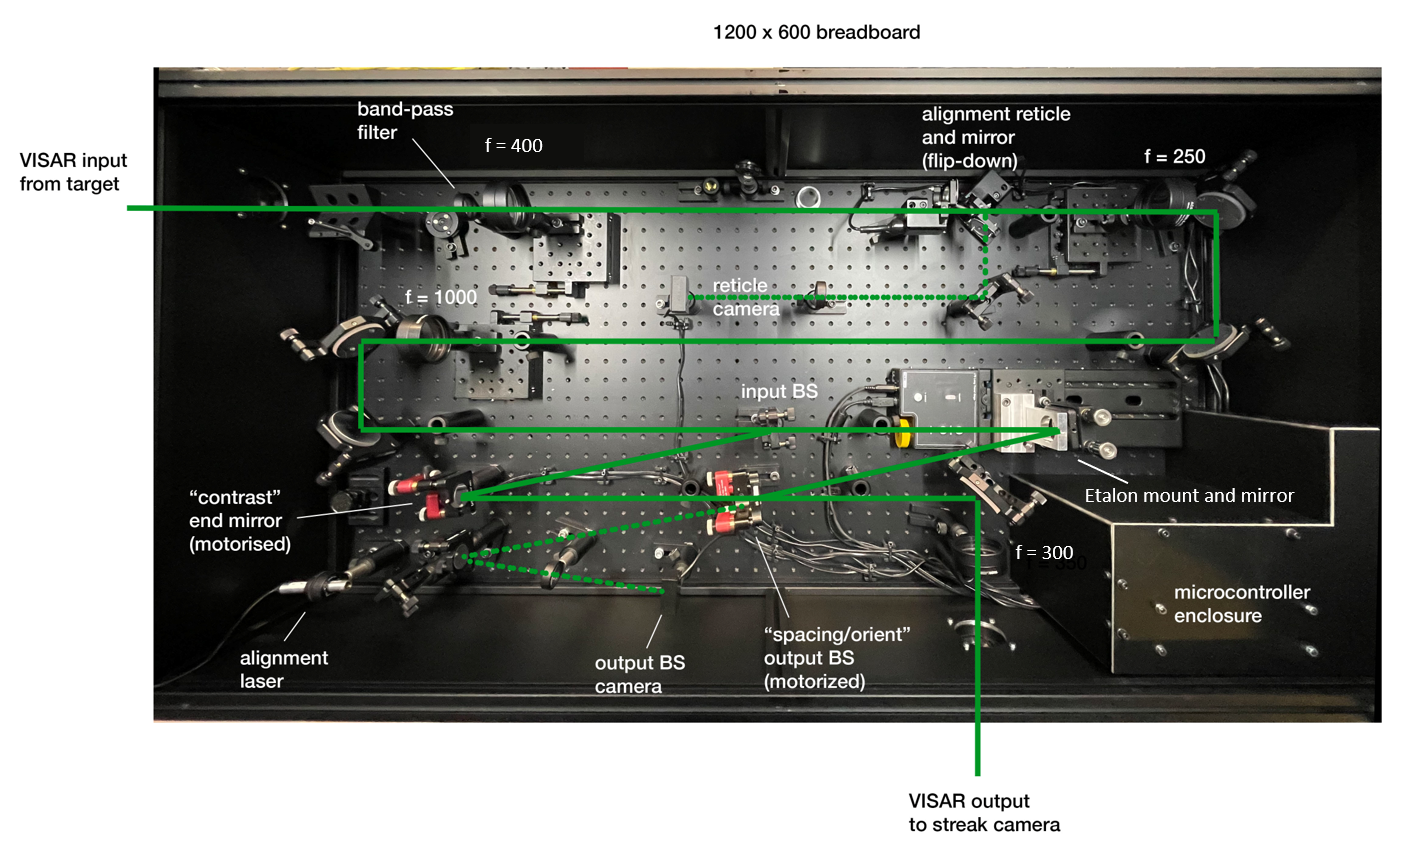
\includegraphics[width=1.0\textwidth]{figures/Experiment/Dan_VISAR.PNG}% Here is how to import EPS art
\caption{\label{fig:Dan_VISAR} The VISAR design used in this experiment (designed and developed by Daniel Eakins). The actual interferometer consists of the components between the input/output beamsplitters, while the other components are used for alignment and to ensure good image contrast. Image provided by Daniel Eakins, with minor changes to labels to reflect the lens setup used in our experiment. }
\end{figure}

The VISAR is internally aligned so that the first flip reticule is positioned in the center of the beampath. This can then easily be used to confirm that the external probe beam entering the VISAR is co-aligned with the system. However, it also serves another important purpose. The etalon and mirror in the delay leg are placed on a piezo-electric motor. As these components are aligned at an angle to the incoming beam, moving them will shift the position of the image. 

For VISAR operation it is required that these two images are aligned. To do this, the etalon is first removed from the delay leg. White light is injected into the VISAR, and the motorised stage on which the mirror and etalon mount sit in the delay leg moved until fringes appear. The white light is incoherent, and so fringes are only observed when the two legs have equal path length - this is sometimes referred to as the `null' or `white-light' position. The system is aligned so that the images are coincident for this seteup, which is confirmed by flipping the reticule into the beam and viewing the images at the output beamsplitter camera.

The etalon is then inserted. This introduces some refraction of the beam, and thus shifts the image. The etalon and mirror are thus translated on the motorised stage until the images are colinear again. This offset can be calculated\footnote{In practice, this offset is found experimentally, and this allows the angle $\theta_h$ to be calculated. This can then be used to accurately determine $\tau$ for the etalon.} by the formula \begin{equation} d = t \left(1 - \frac{\cos\theta_h}{n \cos(\sin^{-1}(\frac{\sin\theta_h}{n}))}\right), \end{equation} where $t$ and $n$ are the thickness and refractive index of the etalon, and $\theta_h$ is the angle of incidence between the laser and the VISAR components \cite{Bolme2013}. This results in a difference in path length which would prevent fringes from being observed with white length; however, the probe laser has a long coherence length, and thus this change is path length is not significant. Ensuring the images are coincident again ensures that the image has good spatial resolution, and also serves to increase fringe contrast - making the signal easier to detect. The time delay that the etalon introduces in a VISAR of this design can be calculated according to \begin{equation} \tau = \frac{2t (n - \frac{1}{n})}{c \cos(\sin^{-1}(\frac{\sin\theta_h}{n}))}, \end{equation} where $c$ is the speed of light \cite{Bolme2013}. 

The main benefit of a Mach-Zehnder design for the VISAR is that the use of two beamsplitters makes it possible to control the image alignment (and thus contrast) and the linear ramp/fringe spacing independently \cite{Celliers2004}. The `contrast mirror' is motorised, and can be adjusted to ensure the best possible overlap between images at the recombination beamsplitter, enabling contrast to be maximised. Independently, the recombination beamsplitter can be rotated to adjust the linear phase ramp, and thus change the number/spacing of the fringes (an important factor in analysing the resulting data). 

\subsubsection{Making shock velocity measurements with VISAR}

The previous descriptions describe how VISAR can be used to dynamically measure the velocity of a moving surface. Measuring shock velocity using VISAR introduces additional complexity, as the surface to be measured is a density interface within the target. To determine what exactly will be measured, it is necessary to consider which surface the VISAR will be reflected from, and it's properties.

The first way to measure shock velocity using VISAR is where the unshocked velocity is transparent to the probe beam, but the shocked material is reflective. In this case, the probe laser can propogate through the unshocked material, and reflect directly off the shock front; this shock front is the measurement surface, and the shock velocity can be measured directly \cite{Celliers2004}. This is the case for alpha-quartz (the reference used in this experiment), which for pressures above $\sim$ 100GPa becomes a conductive fluid with significant reflectivity at 532 \unit{\nano\meter} \cite{Hicks2006a}.

A different approach is required for opaque materials, such as the foam in this experiment. In this case the probe laser will reflect from the stationary front surface of the material, and so will not reach the shock front - the VISAR will thus measure the a zero velocity rather than the shock velocity. However, the VISAR can be used to detect changes to this surface. Fringes will be produced when the surface is intact, but will suddenly disappear when the surface is blown-out and stops reflecting - as occurs at shock breakout. By using steps in the material of known thickness and using the VISAR to identify the time at which the shock transits the steps, it is possible to calculate the average shock velocity through this region.

\subsubsection{VISAR application in this experiment}

In this experiment, the target has a step structure - so that half the rear surface is exposed quartz, and the other is foam. The spot is positioned over this step - so that half of the VISAR image corresponds to signal from the quartz, and the other half from the foam. To illustrate this, some simulated VISAR data has been produced, and is displayed in Figure \ref{fig:VISARToy}. Figure \ref{fig:VISARToy} (a) shows simulated streak images of this VISAR data for two different etalon choices.

\begin{figure}
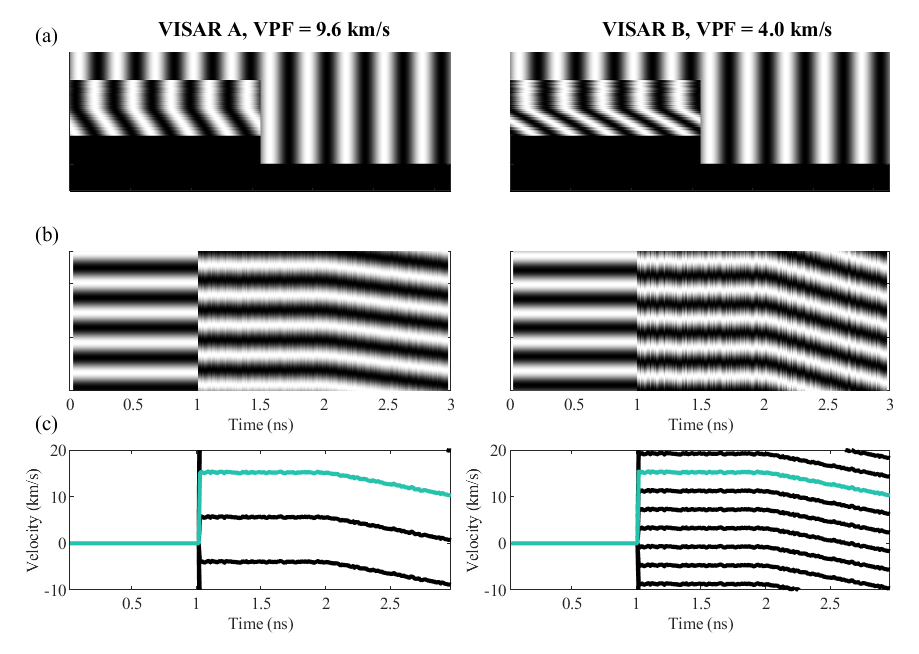
\includegraphics[width=1.0\textwidth]{figures/Experiment/VISARToy.eps}% Here is how to import EPS art
\caption{\label{fig:VISARToy} Simulated VISAR data for two different etalons. Row (a) shows the simulated streak image from each VISAR (where time increases with decreasing $y$ position, and the $x$ dimension represents different positions on the target. In row (b), portion of the data corresponding to the quartz has been selected, rotated, and a timescale added based on the simulated streak window. This has then undergone the filtering and phase unwrapping procedure described in the VISAR analysis section. In row (c), the resulting velocity traces for each VISAR are displayed. The discontinuity could correspond to any integer number of VPFs. However, using two VISARs with different etalons allows for unambiguous determination of the real velocity, since only one of these velocity traces is common to both VISARs (displayed in teal).}
\end{figure}

The underlying data for these simulated images has been chosen to best illustrate the key features/behaviours rather than representing realistic timings or shock profiles, and additional behaviours (such as changes in reflectivity) are neglected for simplicity. A 5 \unit{\nano\second} streak time/measurement window chosen. For the first 1 \unit{\nano\second}, the shock is in the ablator/quartz. The shock is in the quartz for the next 2 \unit{\nano\second}, and in the foam for a further 1 \unit{\nano\second} - breaking out of the rear of the target 1 \unit{\nano\second} before the end of the measurement window. The quartz shock velocity is constant at 15 \unit{\kilo\meter\per\second} for 1 \unit{\nano\second}, and then decays linearly to 10 \unit{\kilo\meter\per\second} over the next 1 \unit{\nano\second}. A small amount of Gaussian noise has been added to these velocities. These values are not representative of what is expected experimentally. The streak images have been created to match the real experimental measurements, with time increasing with decreasing $y$ position in the image, and the $x$ direction representing different points on the target. In this simple model the velocity is constant with position in the two regions; but as the VISAR has spatial resolution, a spatially varying velocity profile could also be measured.

The left half of each streak image in Figure \ref{fig:VISARToy} (a) corresponds to the quartz signal. Initially, the VISAR probe laser will pass through the quartz and initially reflect from the stationary gold layer. When the shock transits through from the gold to the quartz, the laser will begin to reflect from the shock front instead - leading to a sudden jump from a measured velocity of 0 to a measured velocity of $U_{s}^{quartz}$ (15 \unit{\kilo\meter\per\second} in this case). The sudden change in velocity results in a sudden fringe shift. These fringes are static in the new position while the shock velocity is constant, but as the shock velocity begins to decay the fringes are seen to shift smoothly as a function of time. The right side of the image shows the foam signal. The foam is opaque to the probe laser, which continues to reflect off the foam surface - this surface is stationary, and thus the fringe pattern is static.

When the shock breaks out from the quartz, the laser on the quartz side has no surface to reflect off and thus the fringes disappear. The laser on the fringe side continues to reflect off the stationary foam surface until the shock breaks out from this surface too, at which point fringe extinction again occurs. The $y$ position in the streak images can be converted to a time scale, based on the streak time, and thus the shock transit time through the quartz and the foam can be identified from these images, enabling calculation of the average shock velocity.

The quartz velocity can also be obtained as a function of time through VISAR analysis of these images. In Figure \ref{fig:VISARToy} (b), the quartz section of the image has been selected and rotated, and the time scale has been added. The VISAR analysis procedure \footnote{The code I used to do this was based on a VISAR analysis script provided by Daniel Eakins} described in Appendix \ref{appdx: VISAR analysis} was then applied to calculate the shock velocity profiles seen in Figure \ref{fig:VISARToy} (c). While the shock decay is larger than the 4 \unit{\kilo\meter\per\second} VPF of the second VISAR, the extended period this change occurs over means this can easily be resolved. However, the sudden change in shock velocity as the shock enters the quartz leads cannot be resolved, leading in a fringe discontinuity. This could correspond to an infinite number of possible velocity jumps each seperated by an integer multiple of the VPF, as seen for each VISAR in Figure \ref{fig:VISARToy} (c). However, the use of two VISARs with different etalons allows the true velocity profile to be identified, as this profile will be in common between the two images \footnote{Mathematically, this leads to two simultaneous equations: $u = (m_1 + a) \cdot \textrm{VPF}_1$ and $u = (m_2 + b) \cdot \textrm{VPF}_2$, where $u$ is the true velocity, $m_1, m_2$ are the appropriate integer number of fringes missed in the discontinuity, and $a,b$ are the fractional fringe shifts measured in the two streak images. As both signals correspond to the same true velocity, the integers $m$ can be calculated and thus the true velocity determined.}. This is the teal profile displayed in Figure \ref{fig:VISARToy} (c). The shock velocity profile can thus be unambiguously determined.




%It is also necessary to include a translation offset in the delay leg, to account for the refractive index of the etalon. The etalon is placed at an angle to the beam, to avoid reflections from the etalon surfaces introducing interference; this however introduces refraction, which would shift the position of the beam at the recombination beamsplitter. To avoid this, the etalon and mirror in the delay leg are placed on a motorised stage. The etalon is removed, and the mirror translated to find the position corresponding to zero path difference. The etalon is then reinserted, and the mirror/etalon then repositioned until the image is coincident with the null position. this distance, $d = h(1 - 1/n)$ is then recorded. 

%The optical path difference between the delay and non-delay legs is $2(hn - h)$ (as the h thickness of etalon, with optical path $hn$, replaces a distance $h$ of air with a refractive index of 1. The factor 2 comes from the fact that the light passes through this etalon twice). Combining this and the translation offset gives a total path difference of $2h(n - 1/n)$, and thus an optical time delay of $\tau = 2h/c (n - 1/n)$.

%In any interferometer, the fringe frequency is the frequency difference (or beat frequency) of the two legs. In the velocity interferometer, this frequency difference is determined by the time dependent Doppler shift of the reflected light. The light being interfered is a reflection from the measurement surface at a time t1 and a time t1 + $\tau$. The Doppler shift of the reflected beam is dependent on the surface velocity, and thus the frequency difference between these two signals is also linked to the velocity. It is thus clear that the beat frequency will change as a function the velocity of the measurement surface, and thus the fringe pattern will change. However, the operation of the VISAR can be better illustrated by considering the path difference experienced by photons.

%The effect of the VISAR is to interfere photons that were reflected from the measurement surface at different times. At any given time, the photons being interfered at the recombination beamsplitter passed through the seperation beamsplitter at a time $\tau$ apart, and thus reflected from the measurement surface at different times. The measurement surface has a velocity $v(t)$, and thus a position $x(t)$. There will therefore be an additional path difference $\delta x$ between the two paths from the movement of the surface, introducing an additional optical time delay of $2h/c \delta x$.

%If the surface is stationary, then $\delta x$ is constant (zero) and the phase difference between the two legs is constant. The resulting interference pattern is thus unchanging as a function of time. If the surface is moving at a constant velocity, then $\delta x$ is also constant as a function of time. However, if there velocity of the surface is changing, then the phase change will also change, and the fringe pattern will move to reflect this. If the change is large and occurs much faster than the time resolution of the detector, this will result in discontinuities in the fringe pattern.

%The phase difference associated with this delay is given by $\Deltat\phi = kx = x/\Lambda$. As the fringe pattern is given by sin($\Deltat\phi$), one complete fringe corresponds to a phase difference of 2 pi.

\subsection{Streaked Optical Pyrometery} \label{SOP theory}

Streaked Optical Pyrometry enables the temperature of a body to be determined, based on it's thermal emission \cite{Zeldovich1966}. Emmitted light from the target is captured using measurement optics. This light is broadband, but can be filtered down to a narrow wavelength range using appropriate filters. This filtered emission is then recorded on a streak camera, which records the intensity vs time vs a spatial dimension.

%As described in \cite{Miller2007}, the intensity recorded on a streak camera at a given pixel is given by 
%\begin{equation} I = \frac{\Delta t}{G} \int {\Phi_S(\lambda) T_x(\lambda)SR(\lambda) d\lambda}, \end{equation} where $\Delta t$ is the dwell time (the amount of time over which signal is acquired for a given pixel), $G$ is the streak camera gain between photoelectrons and analogue to digital units, $T_x(\lambda)$ is the transmission between the object and the camera, and $SR(\lambda)$ is the SOP response function. $\Phi_S(\lambda)$ is the radiant power from the source. The power from the source that maps to a given pixel can be calculated as 
%\begin{equation} \Phi_S(\lambda) =  \int_{A_{pixel}}{ dA} \int_{\Omega_{lens}} { L_S(\lambda) d\Omega}, \end{equation}
%where $A_{pixel}$ is the source area represented per pixel, and $\Omega_{lens}$ is the solid angle captured by the imaging system. $L_S{\lamba}$ is the spectral radiance of the source. For a given optical setup of the streak camera (i.e. where the target is placed at the same location, the imaging system is not being changed, and the streak camera settings are constant), then these equations can be combined and simplified to 
%\begin{equation} I = \alpha \int {L_S(\lambda) T_x(\lambda)SR(\lambda) d\lambda}, \end{equation} where the proportionality constant $\alpha$ contains a number of variables relating to the specific setup used.

Following the derivation given in \cite{Miller2007}, the intensity recorded on a streak camera at a given pixel is given by \begin{equation} I = G \int {\Delta t} dt \int {\Phi_S(\lambda) T_x(\lambda)SR(\lambda) d\lambda}, \end{equation} where $G$ is a factor proportional to the streak camera gain, $\Delta t$ is the dwell time (the amount of time over which signal is acquired for a given pixel), $T_x(\lambda)$ is the transmission between the object and the camera, and $SR(\lambda)$ is the SOP response function. $\Phi_S(\lambda)$ is the radiant power from the source. The power from the source that maps to a given pixel can be calculated as 
\begin{equation} \Phi_S(\lambda) =  \int_{A_{pixel}}{ dA} \int_{\Omega_{lens}} { L_S(\lambda) d\Omega}, \end{equation}
where $A_{pixel}$ is the source area represented per pixel, and $\Omega_{lens}$ is the solid angle captured by the imaging system. $L_S (\lambda)$ is the spectral radiance of the source. For a given optical setup of the streak camera (i.e. where the target is placed at the same location, the imaging system is not being changed, and the streak camera settings are constant), then these equations can be combined and simplified to 
\begin{equation} I = \frac{B \Delta x W_s \Omega_{lens} G}{\eta M^2} \int {L_S(\lambda) T_x(\lambda)SR(\lambda) d\lambda}, \end{equation} where the variables outside the integral all relate to the specifics of the optical setup and streak camera settings ($B$ is the CCD binning, $W_s$ is the slit width, $\eta$ is the sweep rate, and $M$ is the magnification).

The source is then assumed to emit as a black body, such that the spectral radiance can be calculated using Planck's law, 
\begin{equation} L_S(\lambda) =  \frac{2hc^2}{\lambda^5} \frac{1}{[\exp(\frac{hc}{\lambda T}) - 1]}, \end{equation} where $T$ is the black-body temperature. The SOP signal is therefore given by 
\begin{equation} I = \frac{B \Delta x W_s \Omega_{lens} G}{\eta M^2} \int {\frac{2hc^2}{\lambda^5} \frac{<T_x(\lambda)SR(\lambda)>}{[\exp(\frac{hc}{\lambda T}) - 1]} d\lambda} \end{equation}
The incoming light is filtered down to a narrow wavelength band. Is is thus approximated that the fourier spectrum of the incoming light can be approximated as a delta function, at the central wavelength of this band. This simplifies the SOP signal to
\begin{equation} I = \frac{B \Delta x W_s \Omega_{lens} G}{\eta M^2} \frac{2hc^2}{\lambda_0^5} \frac{T_x SR }{ [\exp(\frac{hc}{\lambda T}) - 1]} , \end{equation}
This equation can then be rearranged to give an expression for temperature in terms of the measured intensity, 
\begin{equation} T = \frac{T_0}{\ln(1 + \frac{A}{I})}, \end{equation}
where $T_0 = \frac{hc}{\lambda_0}$ is a constant, and $A$ is a calibration constant,
\begin{equation} A = \frac{B \Delta x W_s \Omega_{lens} 2hc^2 <T_x SR> G}{\eta M^2 \lambda_0^5} , \end{equation}
which is constant for a constant experimental setup and streak camera settings.

Real samples do not emit as perfect black-bodies. This can be accounted for by factoring in the emissivity of the body \cite{Gregor2016}, which can be calculated as $\eta = 1 - R$, where $R$ is the reflectivity (from Kirchoff's second law, stating that absorption and emissivity are equal for an object in thermal equilibrium \cite{Zeldovich1966}). To account for this in the above derivation, the SOP streak intensity $I$ in replaced in every instance by $I/(1-R)$. This results in an equation for the grey-body temperature of the sample of \begin{equation} T = \frac{T_0}{\ln(1 + \frac{(1-R)A}{I})}. \label{eqn: SOP eqn} \end{equation}

The SOP diagnostic can be absolutely calibrated for a fixed setup, where the components are not regularly changed. This process is outlined for the Omega setup in \cite{Gregor2016}; by making measurements over a series of wavelengths using an absolutely calibrated light source, the different wavelength dependent functions (such as spectral response and transmission) of the camera can be determined. The value of $A$ can then be calculated with confidence for different wavelengths and different camera settings. 

\subsubsection{SOP in this experiment}

In this experiment, SOP was used to measure the signal from both the quartz and foam. However, as the SOP was built from scratch during the experimental run there was not sufficient time nor equipment for an absolute calibration to be performed. Instead, the quartz was used as a known temperature reference, and calibration was performed on-shot.

To do this, the expected quartz shock temperature is required. This was estimated from the VISAR-measured shock velocity using a power law fit from \cite{Millot2015}, \begin{equation} T(K) = 1421.9 + 4.3185 \cdot U_S^{2.9768}, \label{eqn:Temp fit} \end{equation} determined from the experimental data in \cite{Hicks2006}. The corresponding SOP intensity signal could thus be used to calculate the on-shot calibration constant $A$ in equation \ref{eqn: SOP eqn}. With $A$ for the shot determined, the foam SOP intensity could therefore be used to calculate the foam temperature. This on-shot calibration leads to large uncertainty, as error in the shock velocity measurement and the above model both affect the calculated foam temperature.

\subsection{X-ray pinhole camera}
An X-ray pinhole camera imaged the front surface of the target. As the VULCAN beam irradiated the ablator and target, high energy X-rays are emitted in all directions. A diagram showing a pinhole camera is shown in Figure \ref{fig:Pinhole schematic}, while the camera used in the experiment is shown in Figure \ref{fig:Appx-Pinhole} in Appendix \ref{app:2-experimentphotos}. The X-ray pinhole camera consists of a small aperture separated from x-ray sensitive film by a known distance L. The film is shielded so that only x-rays passing through the aperture can reach the screen. This results in a magnification $M$ equal to the ratio $M = L/D$, where D is the distance from the target to the aperture. After each shot, the image plate is scanned to give a two-dimensional image showing the x-ray energy received. The minimum energy of the detected X-rays can be set by placing a filter (a thin film of aluminium) over the aperture.

\begin{figure}
\centering
%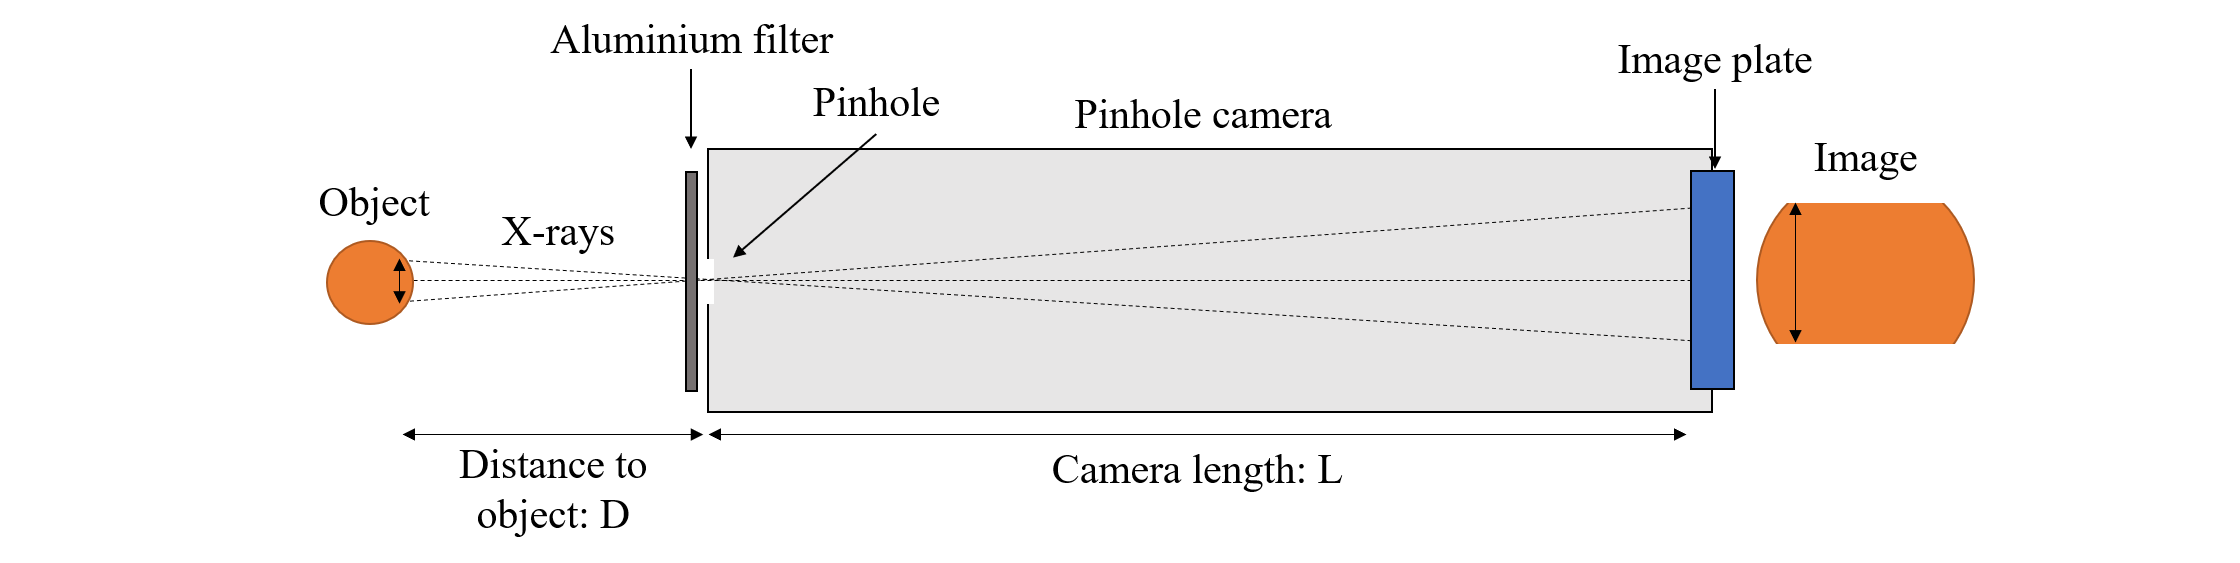
\includegraphics[width=1.0\textwidth]{figures/Experiment/PinholeSchematic2.png}% Here is how to import EPS art
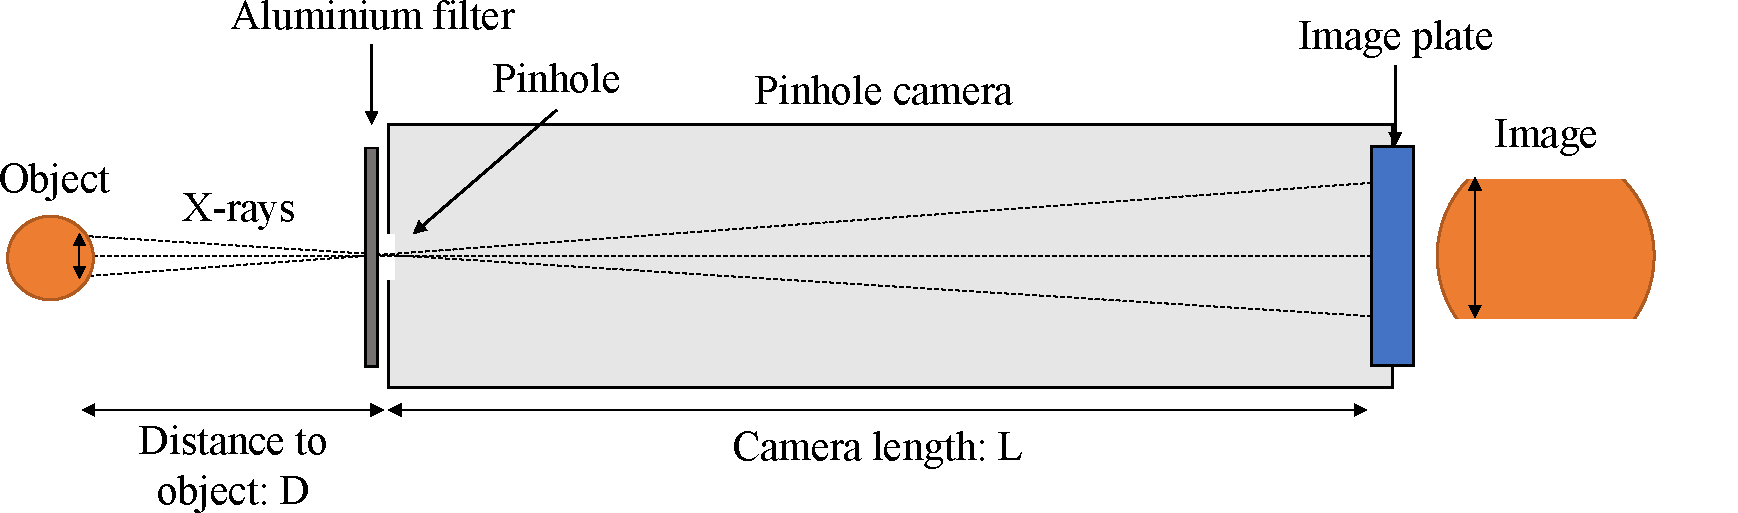
\includegraphics[width=0.8\textwidth]{figures/Experiment/PinholeTest.pdf}% Here is how to import EPS art
\caption{\label{fig:Pinhole schematic} A schematic of a pinhole camera. The distance D between the object and the camera sets the field of view and the magnification.  }
\end{figure}

It is possible to quantify the amount of X-rays received by the image plate, but such an analysis was not necessary/useful for this experiment. Instead, the camera was used to indicate the spatial characteristics of the VULCAN spot. This was useful for confirming where the laser spot hit on the target, that there was a good overlap between the six beams, and to estimate the spot size.

\subsection{Fiducial} \label{Fidu theory}
A fiducial was setup on one of the VISAR streak cameras. A fibre-optic cable was setup behind one of the mirrors in the VULCAN laser chain. These mirrors were slightly lossy, and the fibre `picked-off' some of this parasitic signal. The other end of the fibre was positioned so that it produced a small dot on the side of one of the VISAR streak cameras. The fibre length was such that this parisitic VULCAN signal reached the streak camera in the same streak window that the main signal from the target was detected. This setup can be seen in Figure \ref{fig:Appx-VISARstreaks} in Appendix \ref{app:2-experimentphotos}.

Two-minute shots (low-power VULCAN shots, so-named as they can be fired every two minutes) were performed without a target present, so that the VULCAN pulse could be measured directly on the streak camera. By doing so, the time delay between the VULCAN shot reaching the target and the fiducial signal showing on the streak could be determined. This meant on subsequent full power shots, where the VULCAN pulse could not be seen directly due to the presence of the target, it was possible to calculate the time at which the pulse was applied based on the fiducial signal.

\subsection{Calorimetry}
Calorimeters, which returned a voltage signal based on the fluence of light received, were in place behind a leaky mirror in each of the six beams. These were calibrated to provide an estimate of the energy in each beam for each pulse (one of these was partly blocked by the fiducial, and so returned a low signal - as the six beams were delivering similar energies, an average of the other beam energies was used for this beam when estimating the total pulse energy).

The VULCAN beam is generated at IR, and had to pass through a frequency-doubling crystal to be converted to 527 \unit{\nano\meter}. The facility staff performed a series of calibration shots. On these shots, larger calorimeters were set up in the main beam path to measure the full energy in each beam, while the orientation of the crystal was optimised. This also allowed for calibration of the smaller, on-shot calorimeters; the voltage the parasitic calorimeters measured as a function of the energy measured by the full calorimeters were recorded, and used to find the relationship between voltage and energy, so that the energy of the beam on shot could be calculated.

\subsection{Pulse length}
Photodiodes were placed behind the final set of mirrors in the Vulcan chain (a different set of mirrors to the calorimeters). This can be seen in Figure \ref{fig:Appx-Photodiode} In Appendix \ref{app:2-experimentphotos}. These measured the pulse shape of each beam on every shot, and saved it to an oscilloscope - allowing the pulse length and temporal shape of each beam to be observed.

\section{Preparation for the experiment}

\subsection{Development of the optical setup}

An optical setup was required to collect and transmit the self-emitted light to the SOP. Further optics would also be required to transmit the probe laser to the rear of the target, and to collect the reflected beam and deliver it to the VISAR. 

Both VISAR and SOP were operated normal to the rear target surface. While it is possible to operate VISAR off-axis, this has not previously been done in experiments at these intensities (and would also require a correction to the data). Operating both diagnostics in this configuration meant that a shared optical system would be required to transmit the light from the target to the diagnostics, with a dichroic mirror used to separate the 532 nm light from the self-emission. Similar setups are used on Omega \cite{Miller2007, Gregor2016}.

This optical system had to minimise transmission losses to ensure a strong signal at the diagnostics. In particular, there was a risk that the self-emission could be relatively weak - and thus it was desirable to avoid placing any beam-splitters in the shared optical relay. This meant that the probe laser injection would need to occur prior to the dichroic mirror, resulting in the basic experiment design displayed in Figure \ref{fig:Simple experiment schematic}.

\begin{figure}
  \centering
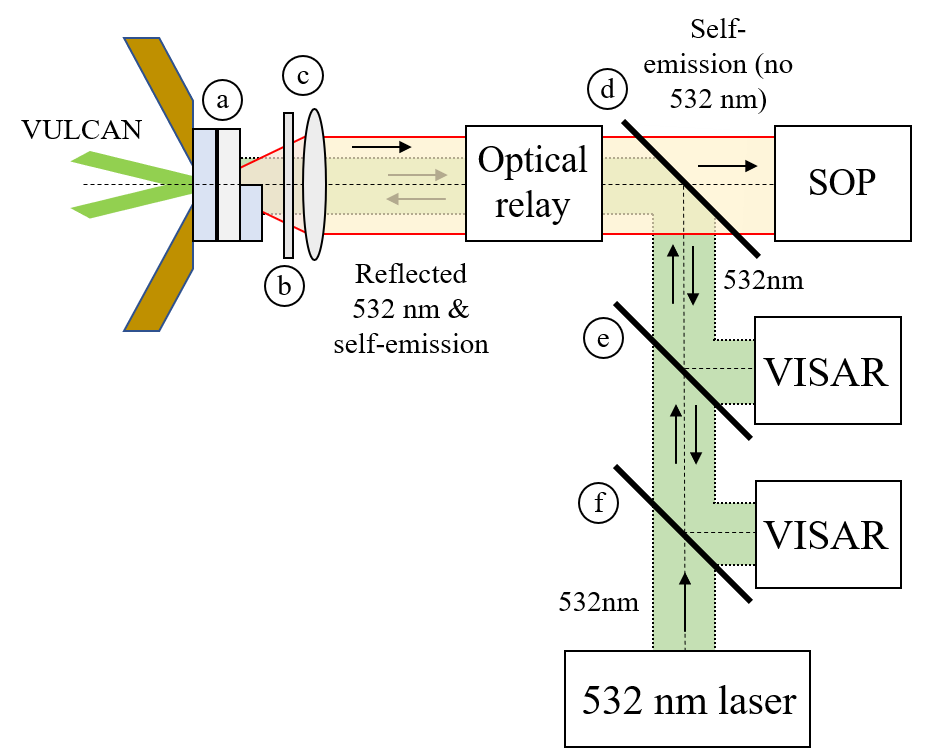
\includegraphics[width=0.8\textwidth]{figures/Experiment/Simple experiment schematic.png}% Here is how to import EPS art
\caption{\label{fig:Simple experiment schematic} A simple schematic of the initially proposed experimental layout. Reflected 532 nm light from a probe laser, and the self-emission, are captured from the target (a) by an objective lens (c) protected by a blast shield (b). This captured light passes through an optical relay, which magnifies it and transports it to the diagnostics. A dichroic mirror (d) reflects the 532 nm light out from the broadband light. This reflected 532 nm light is split and sent to the two VISAR diagnostics via two beamsplitters (e and f). The remaining broadband light passes through the dichroic mirror to the streaked optical pyrometer. The 532 nm laser is injected through the back of the second VISAR beamsplitter, and travels through the full optical relay to illuminate the target. This setup avoids the need for the self-emission to pass through a beamsplitter on it's route from the target to the SOP.  }
\end{figure}

A number of factors needed to be considered in the design of this system:

\begin{itemize}
    \item \textbf{Optical relay spacing}: The spatial configuration of the target chamber and area set limits on the optical relay design. Injecting the probe laser through the VISAR beamsplitter required the laser to be located relatively close to the diagnostics (to avoid a long beam path around the target area). This set constraints on the positions of the optical benches in the target area, and meant that it would be necessary for the optical relay to transmit the light through the south chamber window (which was furthest from the target position). This window was 1.5m away from the target position, with a further 1.3m of window/free space propagation before the optical table would be reached.
    
  \begin{figure}
  \centering
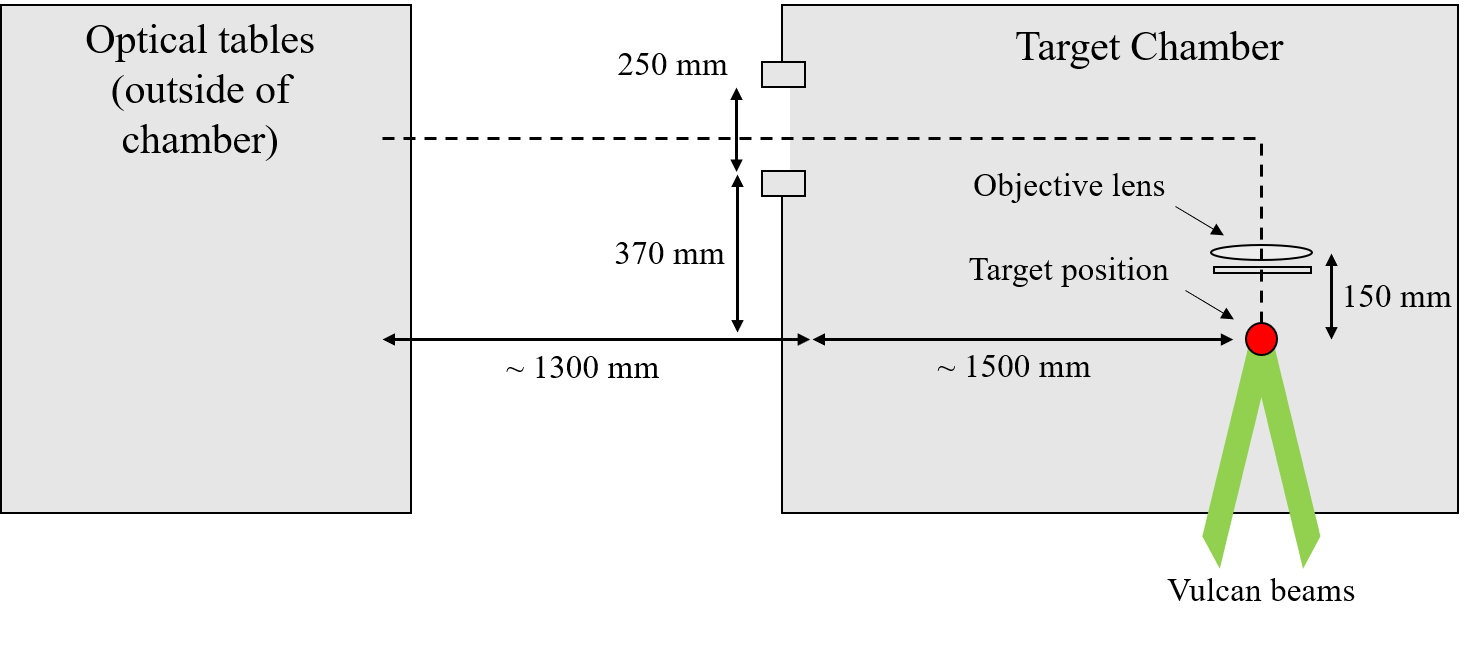
\includegraphics[width=0.8\textwidth]{figures/Experiment/Experiment Spacing.png}% Here is how to import EPS art
\caption{\label{fig:Experiment} A simple schematic (not to scale) showing the spacial considerations for the optical relay. There was a useable distance of $\sim$ 1500 mm of optical table within the chamber before the window. There was then a further $\sim$ 1300 mm gap (in which no lenses could be placed) before the optical tables outside of the chamber, which housed the diagnostics. }
\end{figure}  
    
    \item \textbf{Magnification}: The SOP streak camera had a slit width of 4.46 \unit{\milli\meter}, while the VISAR streaks both had a width of 17.4 \unit{\milli\meter}. The imaged area was 400\unit{\micro\meter} in diameter, and should be magnified to fill as much of this area as possible. The VISAR already had a number of built in lenses (of which only the first could be changed), and so it was necessary to design a system which would provide appropriate magnification for both diagnostics as well as transmitting the beams with minimum losses over the relevant distances.
    
    \item\textbf{Components}: The optical components required for the relay and for the diagnostic systems also needed to be identified and purchased. This included: a dichroic mirror, low-pass and high-pass filters for the SOP, and notch filters (to prevent any 527nm Vulcan noise affecting the VISAR signal). Many of these components, as well as the optical components within the VISAR, were only available in 1-inch versions - which set limits on the beamsize.
    
    \item \textbf{Diagnostic positioning}: Finally, it was necessary to consider how the diagnostics and beam paths would actually fit on the optical table. The VISARs in particular were large pre-assembled systems with fixed entry points for the beam path. The 1-inch optical components meant it was necessary to minimise the distances between the VISARs and the final lens in the optical relay to avoid transmission losses, but this was challenging to achieve practically.
    
\end{itemize}

To assist with this design work, a Matlab script was produced to perform ray-tracing (using simple geometrical optics) of light through a lens system. A number of setups were explored using this code to find a system which minimised losses while being compatible with the above considerations. The final design achieved this, with transmission (according to the simple approximations used within the code) above 99\% from the first lens to the target. Details of the operation of this code are provided in Appendix \ref{appdx: Ray Tracing}.

Figure \ref{fig:Full experiment schematic} shows a full schematic of the experiment. The optical relay consists of 5 lenses (L1 to L5). The dichroic mirror then takes the collimated beam, and sends the signal to the SOP/VISARs. The SOP consists of a 400 nm long pass filter and 500 nm short pass filter, leaving only 400 - 500 nm wavelengths, before a final lens S1 focusses the beam on to the streak camera. Beamsplitters send the VISAR beam into the VISAR system (the `VISAR' here is used to refer to the full system shown in Figure \ref{fig:Dan_VISAR}, rather than just the interferometer). The beam passes through a notch filter, followed by the 4 lenses within the VISARs (and the interferometer, which is not shown), before being focussed onto the beam splitter by lens V5 (and further focussed in the vertical direction by the cylindrical lens V6). The lens spacing can be seen on the CAD models in the appendix. The spacing between focussing pairs is fixed by the focal distances of the lenses. There was some flexibility in the spacing between L1 \& L2 and L3 \& L4; however, the distance between L5 \& V1 for each VISAR had to be kept below 1m to avoid losses (otherwise the beam would be too large for the 1 inch components inside the VISAR), and the distance from V4 to the VISAR streak camera also needed to be under 1m. The short pass filter (c) was also a 1 inch component, and so it was important to place this close to the dichroic mirror.

\begin{figure}
%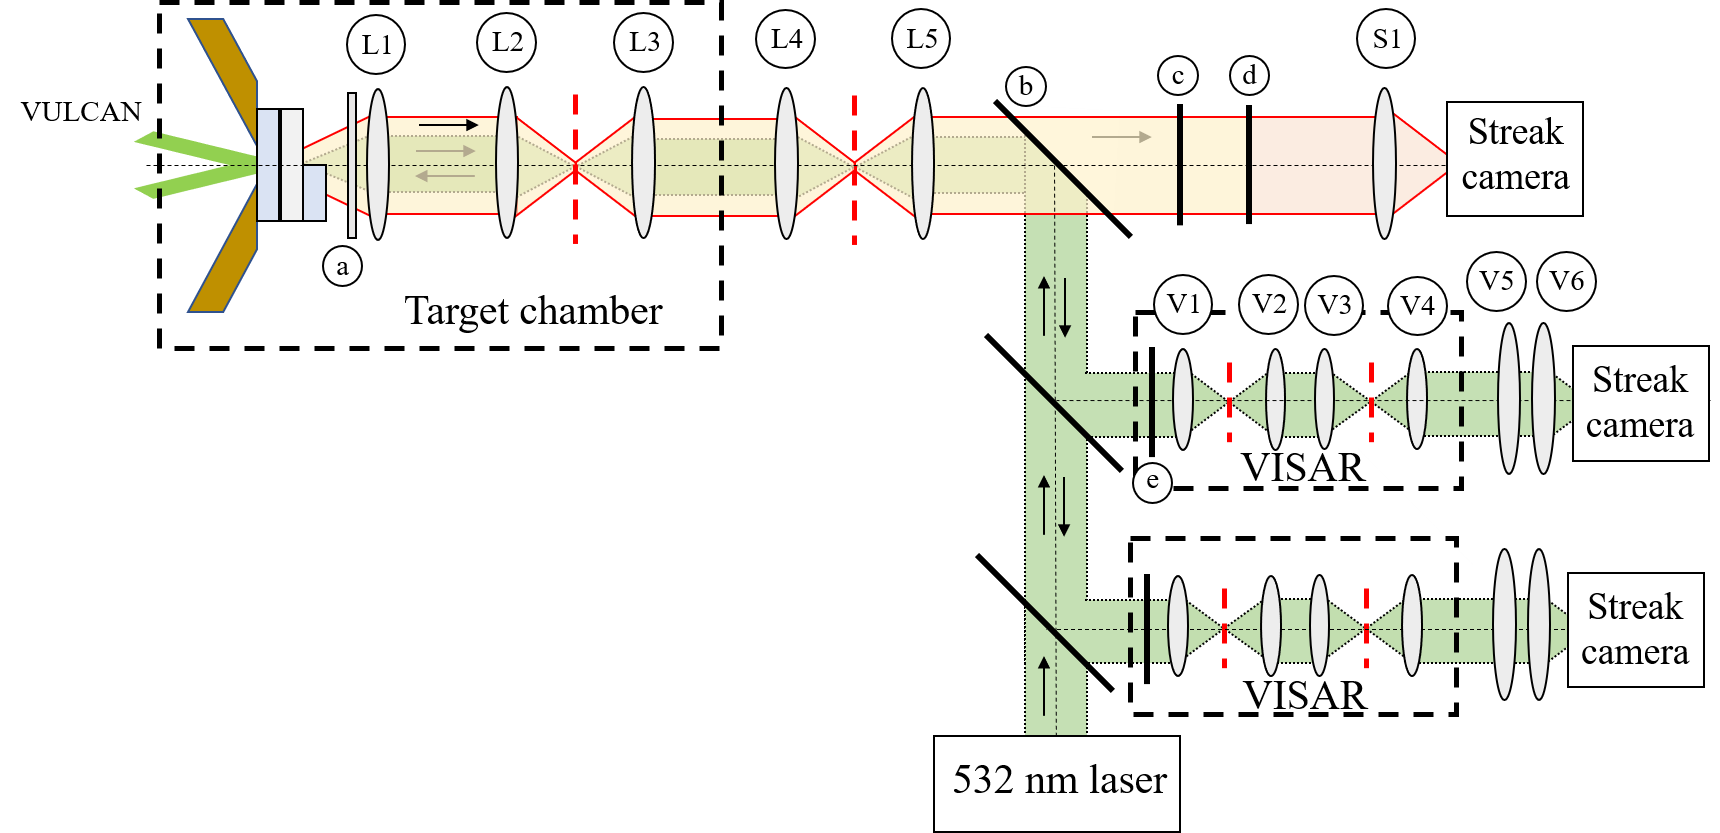
\includegraphics[width=1.0\textwidth]{figures/Experiment/Full experiment schematic.png}% Here is how to import EPS art
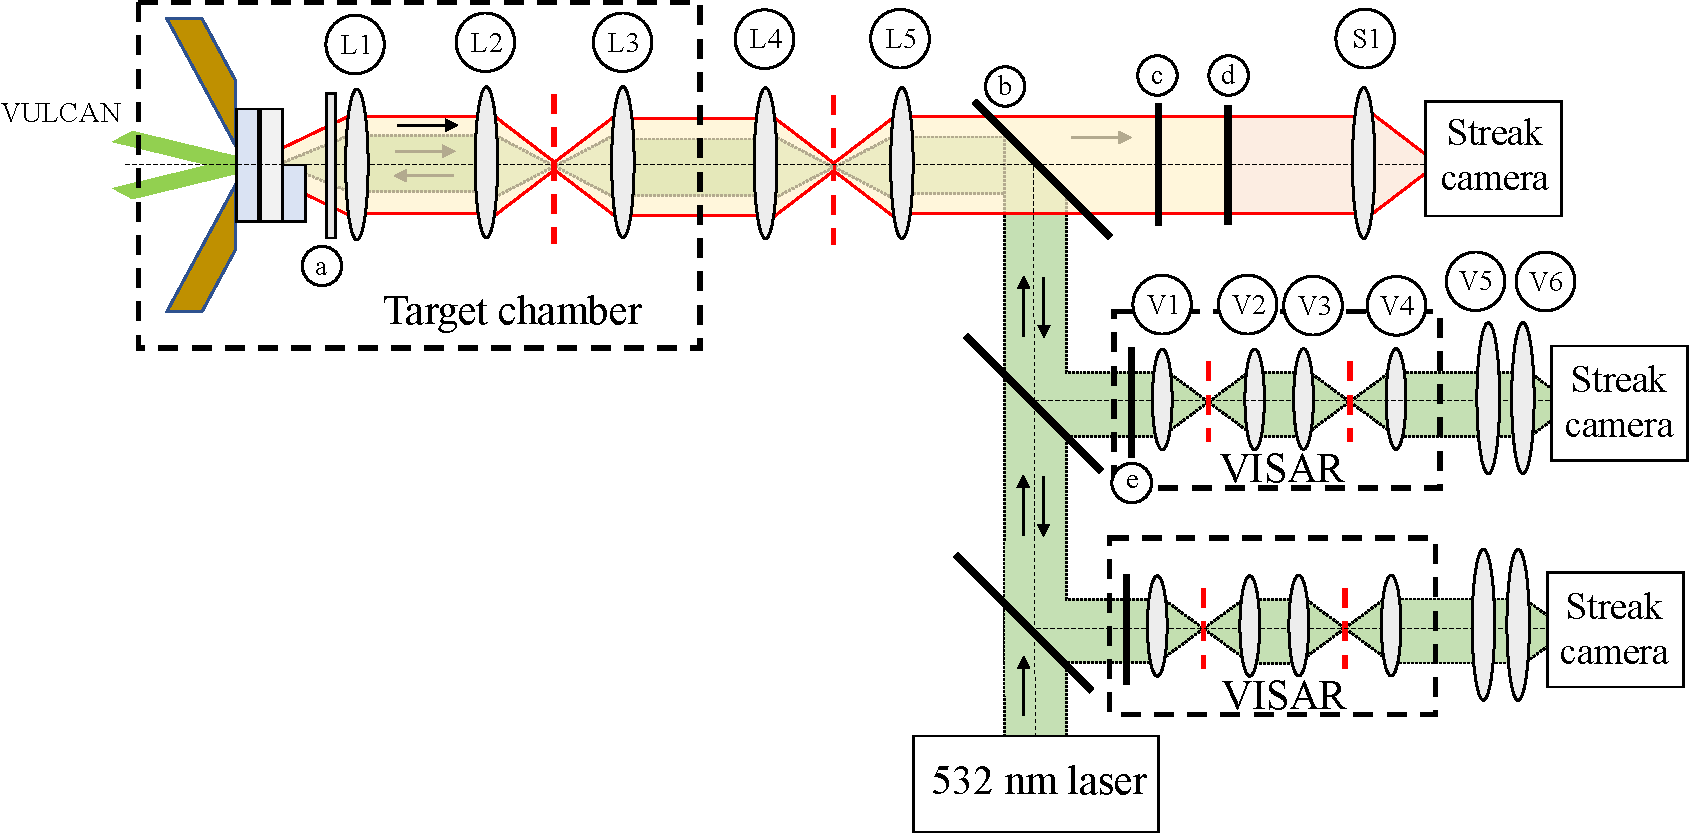
\includegraphics[width=1.0\textwidth]{figures/Experiment/Full Experiment Schematic.pdf}% Here is how to import EPS art
\caption{\label{fig:Full experiment schematic} The full proposed schematic. Lenses labelled 'L' form the optical relay, while those labelled 'S' are part of the SOP and 'V' are part of the VISAR. The two VISARs are identical in terms of components. The dashed red lines represent the positions of image planes. The interferometer in the VISAR is not pictured (it can be viewed in Figure \ref{fig:Dan_VISAR}), but is positioned so that the second beamsplitter is positioned at the second image plane. The focal lengths are as follows: L1 = 150mm, L2 = 700mm, L3 = 500mm, L4 = 700mm, L5 = 250mm, S1 = 300mm, V1 = 400mm, V2 = 250mm, V3 = 1000mm, V4 = 300mm, V5 = 300mm, V6 = 200mm (cylindrical). Also indicated are the other components in the beamline: a blast shield to protect the objective lens (a), the dichroic mirror (b), the short-pass (c) and long-pass filters (d) for the SOP, and notch filters (e) for the VISARs.}
\end{figure}

Figure \ref{fig:Original CAD} shows the designed arrangement of this setup, which allows all the spatial requirements to be satisfied. Figure \ref{fig:Ray trace} then shows the output of the ray tracing script for the target to SOP and target to the second (furthest) VISAR. 

\begin{figure}
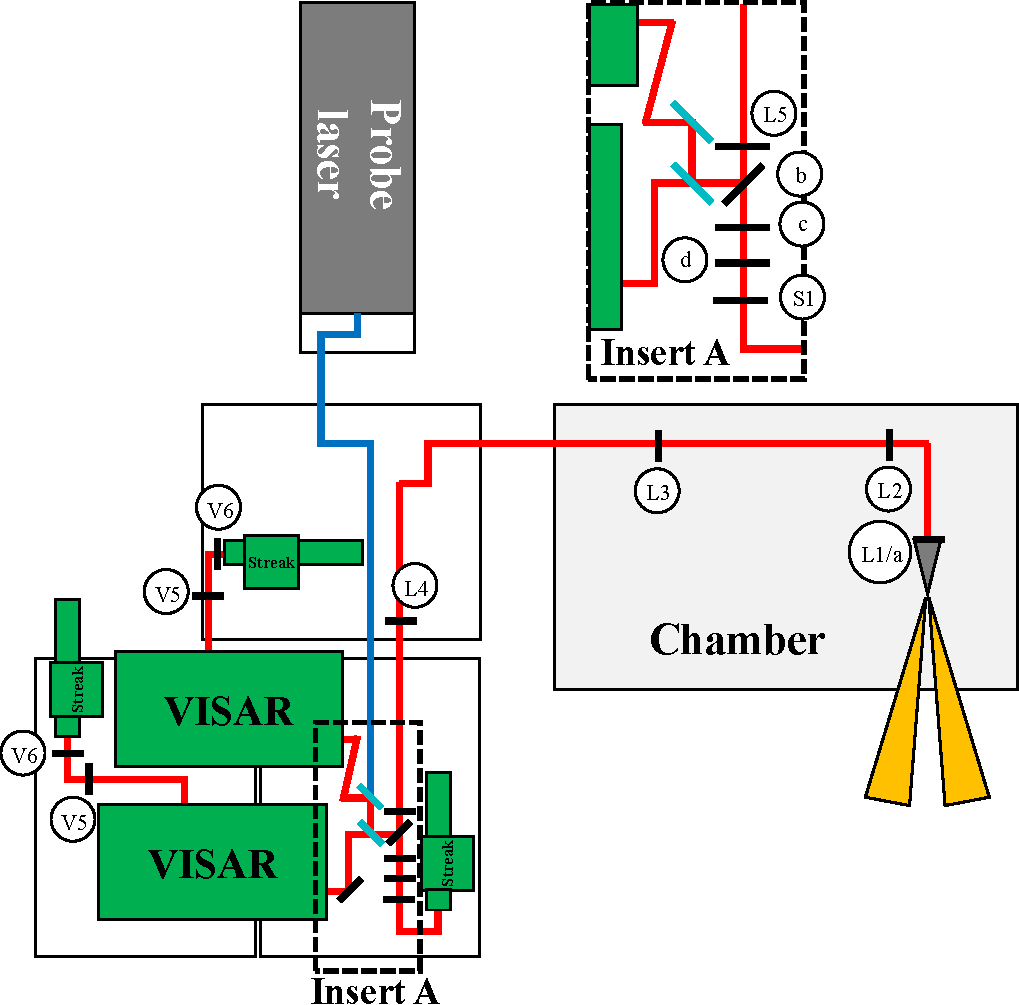
\includegraphics[width=1.0\textwidth]{figures/Experiment/OriginalSetup.pdf}% Here is how to import EPS art
\caption{\label{fig:Original CAD} A schematic showing the spatial arrangement of the experimental equipment (not quite to scale, but close enough to be representative). The white boxes indicate the optical tables on which components could be placed. Mirrors are not shown, but are present when the beam turns. Beamsplitters are displayed in teal; all other components are labelled as described in Figure \ref{fig:Full experiment schematic}. The insert shows a close up view of the section in the dashed black box. The beamline colors are used to correspond to the CAD models in the appendix, rather than representing anything physical.}
\end{figure}


\begin{figure}
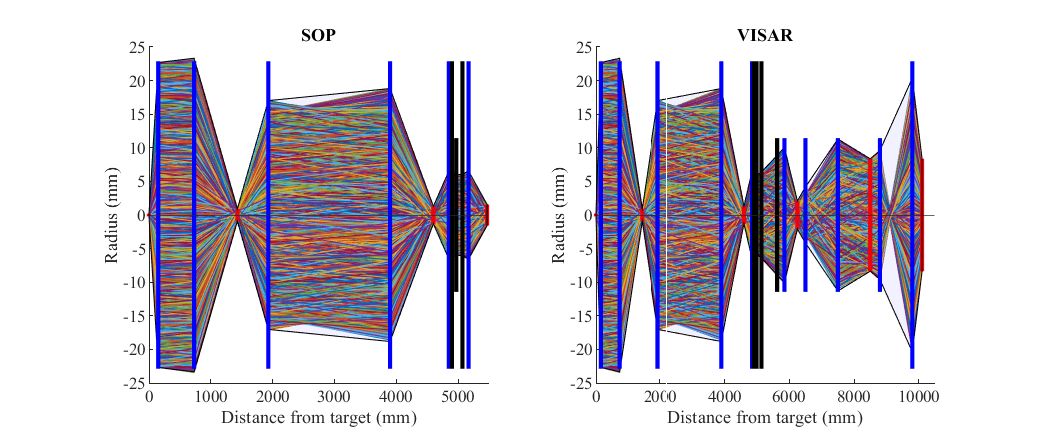
\includegraphics[width=1.0\textwidth]{figures/Experiment/RayTracing.eps}% Here is how to import EPS art
\caption{\label{fig:Ray trace} Ray tracing simulations from the target through to the SOP and VISAR. The components are placed with the real experimental spacing. Lenses are represented by blue lines, while other components (dichroic mirror, beamsplitters, filters) are represented by black lines. 10,000 rays are generated, each at a random position on the target and with a random angle. These rays are propagated through the system according to simple geometric optics through thin lenses. At each component position, the radial position of each beam is compared to the component size; if it is bigger, the ray is considered `lost'. This approach suggests transmission through the system greater than 99\% for both the VISARs and SOP (with the small losses occuring between L1 and L2).}
\end{figure}

\subsection{Target design and hydrodynamic simulations} \label{Target Design}

\subsubsection{Layer choice and thickness}

The initially proposed target was based on multi-layer step target desgins successfully used in previous experiments \cite{Falk2014a, Falk2020}. The initial proposal used an aluminium layer as the reference, but this was replaced with quartz so that the velocity of the shock could be measured directly using the VISAR \footnote{The original proposal had suggested that the VISAR could be used to measure the free surface velocity of the aluminium and foam. Under this approach, the VISAR reflects from the rear of an opaque target. The target is shocked, and the shockwave reaches the rear surface, which undergoes free surface expansion. The free surface velocity is measured by the VISAR; this is generally approximated as being twice the particle velocity within the shocked medium. This is a common approach at lower pressures, but it is not possible in this regime - as the shocked material becomes a plasma, the rear surface is destroyed and thus the free surface velocity cannot be measured. As such, the target design was changed to replace the aluminium with quartz, and the foam shock velocity was instead determined from the transit time}. The four layers and step structure led to a relatively complicated target.

The thicknesses of the different layers were influenced by a number of factors. These are listed below:

\begin{itemize}
    \item \textbf{VULCAN pulse length/energy capabilities}: In order to ensure a sustained shock, it was intended that the laser pulse should last until the shock broke out from the rear of the target. There was an upper limit on how long VULCAN could sustain a pulse for (particularly at high intensity, where high energy is required), and this therefore prevented very thick targets with long shock propagation times.
    \item \textbf{Secondary shocks}: Hydrodynamic simulations showed that when the shock crossed from the gold layer into the quartz, a release wave would propagate back through the target. Upon reaching the ablation front, this would generate a second shock which would travel through the target. Depending on intensity/target thickness, this secondary shock could catch up and merge with the primary shock. This would mean the shock strength would change, which would prohibit the use of the impedance matching calculation. This effect was heavily influenced by the thickness of the different layers, and needed to be avoided. An example of this behaviour can be seen in FIGURE.
    \item \textbf{Fabrication constraints}: Target fabrication indicated that the 40~\unit{\micro\meter} was the minimum thickness of quartz/foam that they would be able to produce.
    \item \textbf{Preheating}: The gold layer would need to be sufficiently thick to prevent preheating of the quartz/foam. 
    \item \textbf{Avoiding direct laser heating of gold}: The ablator needed to be sufficiently thick so that the ablation front remained in this layer throughout the laser pulse, and thus the gold did not undergo direct laser heating.
\end{itemize}

Hydrodynamic simulations were performed to find the optimal target design. The minimum 40~\unit{\micro\meter} thickness for the quartz and foam was chosen to mitigate the pulse length concerns. This also was required for the second shock; the thicker the quartz/foam layers were, the more distance there was for the second shock to catch the primary shock in. 40~\unit{\micro\meter} quartz/foam thickness the second shock was already a significant problem. 

Increasing the gold and ablator thicknesses were both found to delay the second shock, improving this issue (the gold/quartz interface was moved further from the ablation front, which meant the second shock (which has to travel this distance twice once it is generated at this interface) had a longer distance to travel relative to the first). Simulations were performed investigating the potential gold/ablator thicknesses that could be used, and the impact this would have on the required laser pulse time/energy at different intensities.

The selected design used a 40~\unit{\micro\meter} ablator, and a 3~\unit{\micro\meter} gold layer. In Hyades, this led to the required pulse times/pulse energies as a function of intensity seen in Figure \ref{fig:VULCAN energy} - remaining under the 600 J maximum energy of VULCAN for the full planned intensity range \footnote{In spherical hydrodynamic simulations a multiplier is applied to the incoming laser energy to account for losses such as cross-beam energy transfer. CBET is likely to be less important for this setup, but there likely would be some loss. The simulations presented in this section do not include such a multiplier, and so it's likely that the shots would require a larger energy/pulse time for a given intensity. However, as the highest intensity in Figure \ref{fig:VULCAN energy} requires only 500 J as opposed to the 600 J VULCAN can deliver, there is some additional energy available to account for this. }. The target did not experience second shock merger over this intensity range. The simulations also suggested that the ablation front remained in the ablator for all of these intensities, and that the 3\unit{\micro\meter} gold layer would prevent preheating of the foam to less than 10K. Hydrodynamic simulations cannot be expected to describe preheating with high accuracy, as they do not include many of the laser plasma effects; however, previous experiments have used similar gold thicknesses, and did not report substantial amounts of preheat - suggesting that this thickness would be appropriate.


\begin{figure}[hbt!]
\centering
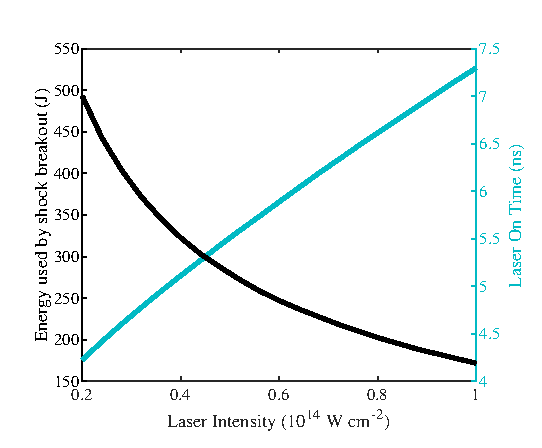
\includegraphics[width=0.6\textwidth]{figures/Experiment/EnergyandPulsetimes_edit.eps}% Here is how to import EPS art
\caption{\label{fig:VULCAN energy} The required VULCAN pulse times as a function of intensity, if the pulse is to be applied until shock breakout from the rear of the target, as simulated in HYADES. The shock breakout time is identified from simulation at each intensity, which defines the required pulse time. The energy of this pulse (given the known intensity and required pulse time) can also then be calculated. There is an inverse relationship between these two parameters; higher intensities result in faster shocks (and thus shorter required pulse lengths), but the increased intensity also means that the required energy of the pulse is higher (i.e. the pulse length does not reduce by enough to balance the increased power).}
\end{figure}

\subsubsection{Additional considerations}

There were also a number of practical concerns with the target assembly. Firstly, it was key to the experiment that no glue layers were used in the target, for a number of reasons. Firstly, there was concern that glue might wick into the foam, which would change it's behaviour. Secondly, a glue layer between the quartz and the foam would prevent impedance matching being performed, as these two materials would not be in contact. Finally, a glue layer between the gold and the quartz would make it difficult to determine when the shock entered the quartz from the glue layer. This meant that the target had to be constructed without glue. The manufacture of the targets was handled by CLF target fabrication (particularly Chris Spindloe, Sam Irving, David Haddock, and Donna Wyatt). The ablator and gold coatings were grown directly on to the quartz, so that no glue was required here. The foam was placed in position on the quartz, so that one foam edge was centered on the quartz piece (giving the step structure). The foam was then `tacked' to the quartz with glue at the corners - this was sufficiently far from the center of the target that there would be no glue between the layers in the shocked/imaged region.

Secondly, coatings were required for the quartz. An anti-reflection coating was requested on the quartz surfaces, to prevent spurious reflections and `ghost fringes' (where reflections from other surfaces lead to interference and persistent fringes in the data).

\subsection{Hydrodynamic simulations}

The hydrodynamic simulations mentioned in the previous section also enabled the expected conditions in the quartz/foam to be investigated. A selection of the key shock variables can be seen in Figure \ref{fig:PreExpHydro}. These simulations were performed in Hyades and were used to inform etalon selection, as well as confirming that the quartz pressure was sufficient for a reflective shock front. Experimental collaborators also ran simulations of this in Multi, Helios, and FLASH, and good agreement was observed (a comparison between these codes can be seen for the post-experiment simulations).

\begin{figure}[hbt!]
\centering
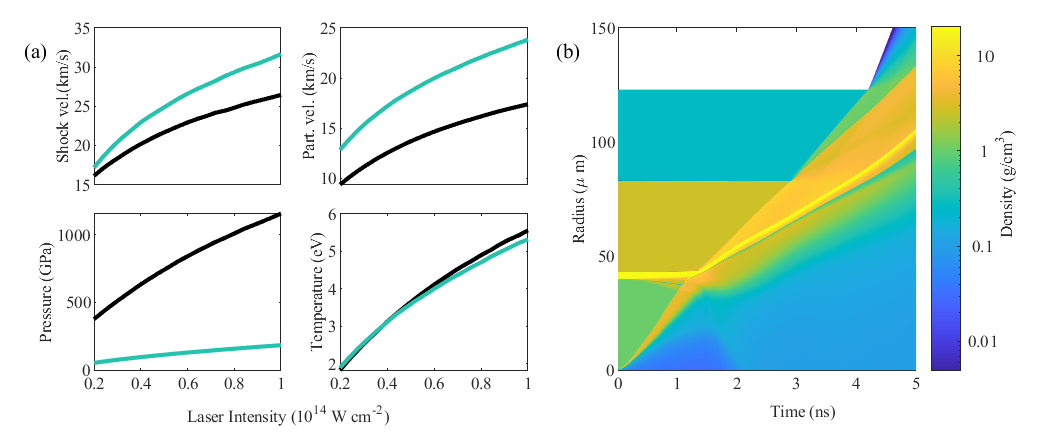
\includegraphics[width=1\textwidth]{figures/Experiment/PreExperimentHydro.eps}% Here is how to import EPS art
\caption{\label{fig:PreExpHydro} Shock conditions in the quartz (black) and foam (teal) as a function of intensity (a), and a density plot showing shock propagation through the target for an intensity of \num{1e14} \unit{\W\per\centi\meter\squared}. The quartz shock velocity informed decisions on the required etalons. The shock pressure in the quartz is also confirmed to be above the threshold for a reflective shock for the full range of simulated intensities.}
\end{figure}

Two-dimensional simulations of this setup were also performed to ensure that the shock was planar and that similar shock behaviour was observed in higher dimensions. The simulations presented in this section were performed in h2D (the two-dimensional version of Hyades). This is a Lagrangian code and as such suffers from mesh tangling, where the movement of the different zones can cause the mesh to become distorted and prevent the simulation from continuing. This requires the user to manually rezone the problem, and frequently also resulted in the simulation code crashing. After a number of iterations a sufficiently detailed simulation was ran to completion. Other 2D simulations were performed in Multi-2D and FLASH 2D by the other collaborators and were used to confirm these results; as these codes were ran with more success they were used instead of h2D for the post-shot simulations, and will be discussed in more detail in that section.

In h2D, a simple four layer target was simulated without a step in the foam. This was sufficient to measure shock propagation and to estimate the shock variables, as well as to indicate the shock planarity. 2D FLASH simulations (performed by other collaborators) were used to confirm that the step did not have a significant impact on the shock behaviour (this can be seen in later sections). h2D is an axisymmetric code, and so the target is simulated as a cylinder where the shock propagates along the long axis. R=0 is the axis of symmetry, and the 2D plane can be rotated around this axis to produce the full target (this also means that any off-axis beams are actually rings of laser light). The laser was simulated as 3 beams at -25$^{\circ}$, 0$^{\circ}$, and 25$^{\circ}$ to the target normal. Given the real experimental configuration (three pairs of two beams) a simulated setup consisting of two beams at 6$^{\circ}$ and -6$^{\circ}$ would also have been valid, but the three beam setup was chosen as included larger deviations from target normal, and would thus be more likely to exhibit changes from 1D behaviour. 

Figure \ref{fig:H2DSchematic} shows a number of schematics highlighting how the simulated setup works and compares to the real experimental configuration. Figure \ref{fig:H2DSchematic} (a) shows the real laser setup (not to scale), with the 3D configuration of the six beams. This cannot be accurately simulated in 3D. Figure \ref{fig:H2DSchematic} (b) shows the 2D simulation. Three laser beams are simulated by specifying a number of `rays' with an initial angle and position. The rays were created using a `random-to-uniform' lens-to-target mapping in Matlab. 10,000 uniformly spaced points were generated over the laser spot at the target, and for each point an incident ray was generated. Each ray was given an origin position at random, corresponding to a position on the lens for one of the three laser beams (considering the real lens size and lens-to-target distances). This method ensures that uniform illumination of the laser spot is achieved with the finite number of beams, while also using a random mapping to ensure behaviours such as defocussing past the laser focus. The energy of the ray was scaled according to the square of it's radial position at the target; this accounted for the axisymmetric symmetry, and the fact that a ray incident on a higher radial position is spread over a much larger area if the 2D slice is converted to a 3D cylinder. While only positive radii are simulated, as the rays are described at a single point (on the target face), it is possible to include rays which would have originated on the other side of the Z-axis. This is shown in Figure \ref{fig:H2DSchematic} (c) where the simulation is reflected around the z axis, and it is shown that the rays shown in (b) do in fact originate from all 3 beams. Finally, Figure \ref{fig:H2DSchematic} (d) shows the rotation of the simulated setup in (b) around the axis. Here, it can be seen that this rotation means that the off-axis beams in fact represent a hollow cone of incoming laser light.

%\begin{figure}[hbt!]
%\centering
%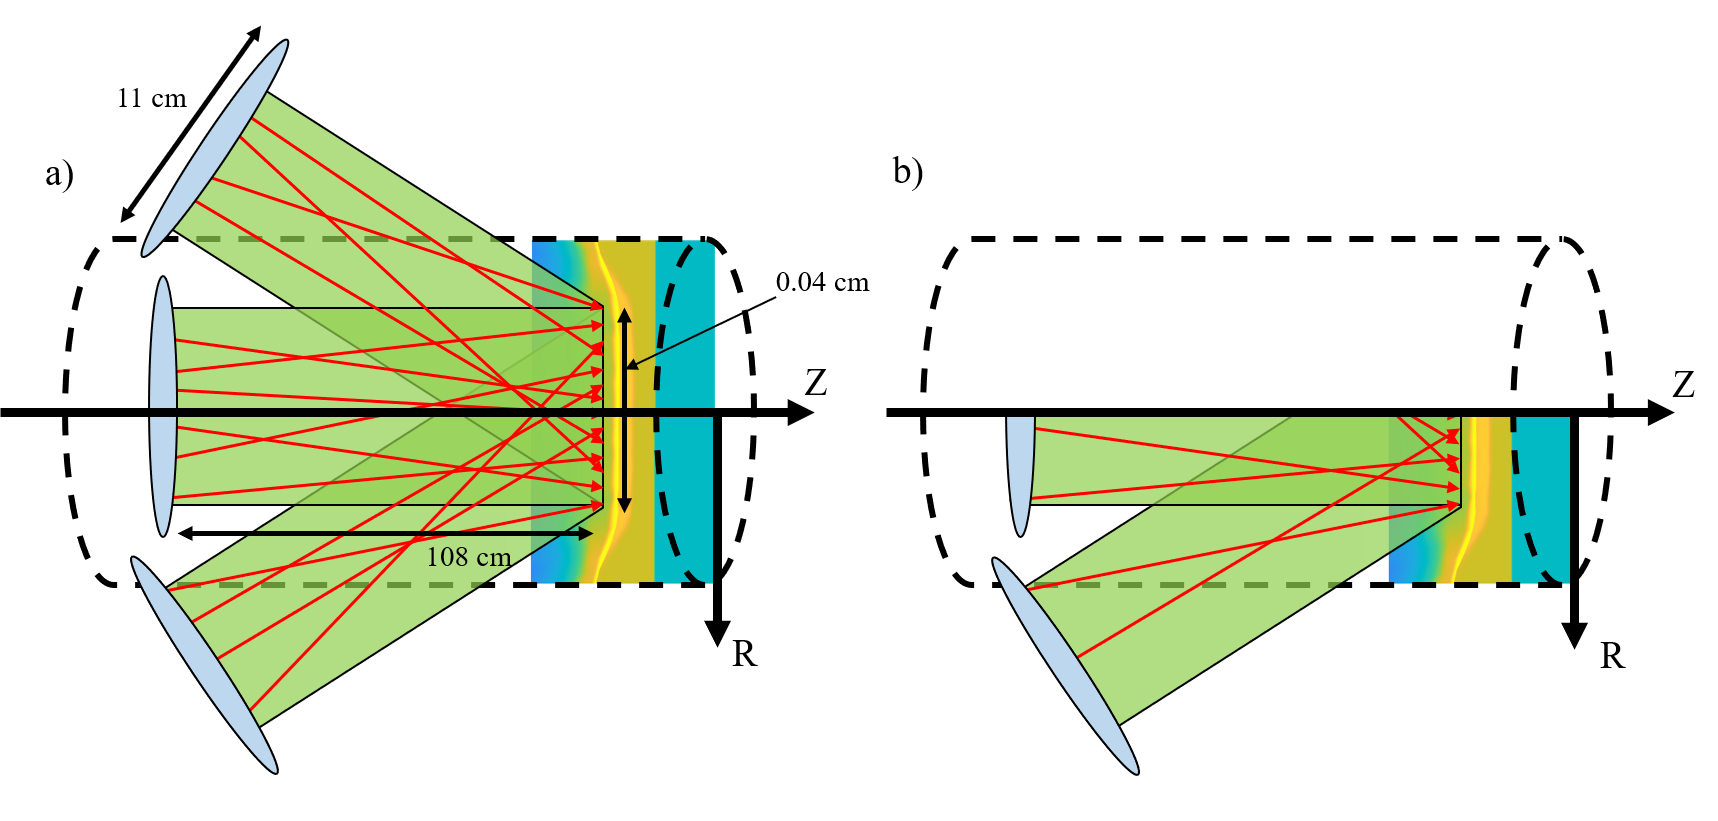
\includegraphics[width=1\textwidth]{figures/Experiment/H2DSchematic2.png}% Here is how to import EPS art
%\caption{\label{fig:H2DSchematic} A schematic (not to scale) showing the simulated setup. In a), the full concept is shown. Three three beams produce a 400 \unit{\micro\meter} laser spot on the target. These beams are described by a series of rays originating from three 11 cm diameter lenses 108 cm from the target (these dimensions are accurate to the experiment). A small number of example rays are demonstrated by the red arrows. The rays are evenly spaced at the laser spot, but each is mapped to a random origin point on one of three lenses, which ensures the beam would defocus appropriately beyond the focal plane (the lenses are much larger than the focal spot, and so in practice these beams are heavily focussed - unlike in the schematic). For the purposes of the simulation, the target is considered to be a cylinder. R and Z are simulated, but the azimuthal behaviour is neglected (due to the 2D nature of the simulation). In b), the section included in the simulation is shown. Half the target diameter is simulated, and this can be extruded round the azimuth to produce the full target. Only the rays incident on this half of the target are included - but as the rays are specified at the target surface, it is possible to include rays that would have originated on the other side of the Z-axis. As the rays would also be uniform around the azimuth, the two off-axis beams would actually be simulated as a cone of incoming laser light.}
%\end{figure}

\begin{figure}[hbt!]
\centering
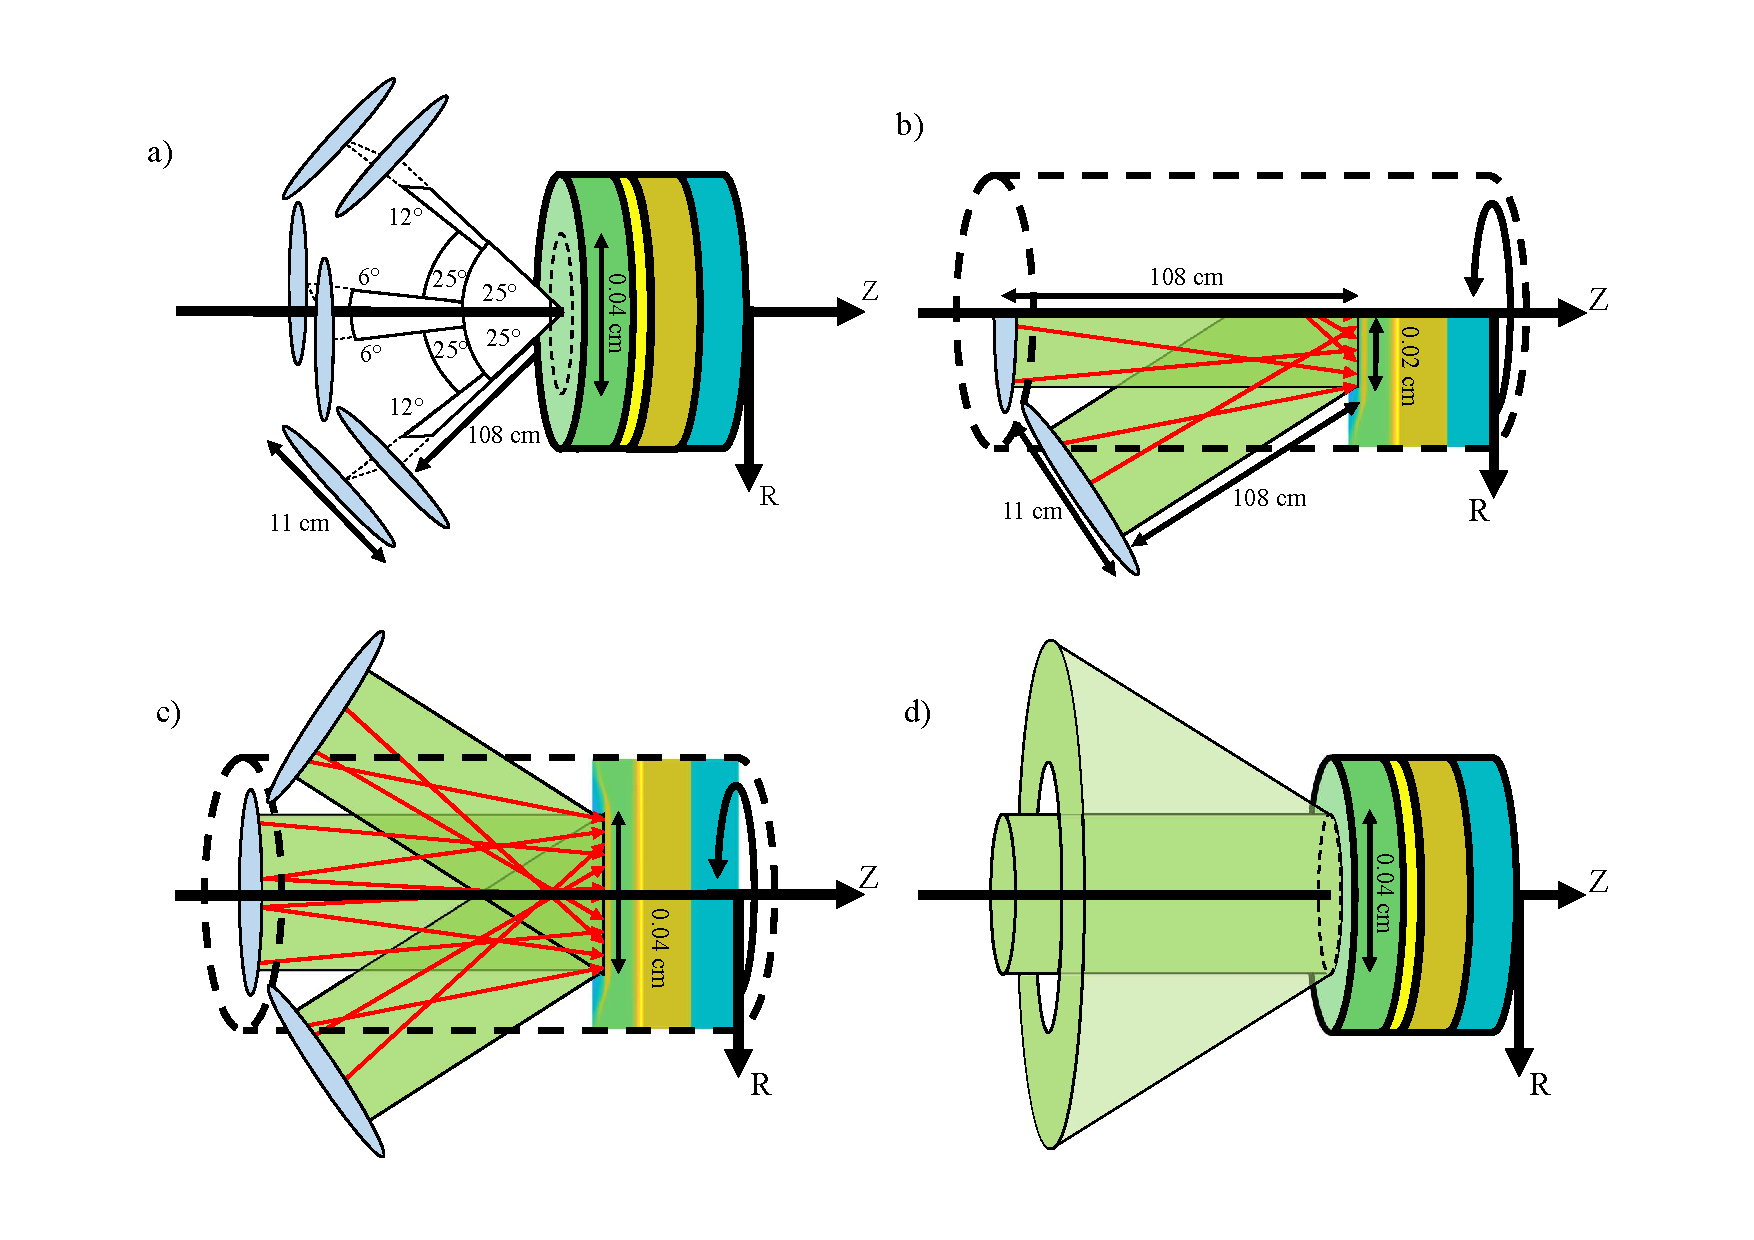
\includegraphics[width=1\textwidth]{figures/Experiment/H2DSchematic.pdf}% Here is how to import EPS art
\caption{\label{fig:H2DSchematic} A schematic (not to scale) showing how the setup is simulated in h2D. a) The real experimental layout of the 6 beams. The beams are arranged in three planes at -25$^{\circ}$, 0$^{\circ}$, and 25$^{\circ}$ to the horizontal, with each plane containing two beams at 6$^{\circ}$ and -6$^{\circ}$ to the vertical. Each beam is 11 \unit{\centi\meter} in diameter at the lens, which is 108 \unit{\centi\meter} from the target, and is focused to a 400 \unit{\micro\meter} meter spot. b) The h2D simulation. This is done in 2D with cylindrical symmetry. The laser is described using rays, which are mapped from a random position on one of three lenses (at -25$^{\circ}$, 0$^{\circ}$, and 25$^{\circ}$ to the horizontal, at the correct distance) to a uniform grid of points in the laser spot. c) The h2D simulation has been reflected around the x-axis, and the rays traced back to show their sources. As the rays are generated in the laser spot, the configuration in (b) allows for rays to cross the z-axis, even though this lens would not be in the area included in the simulation. d) The 3D extrapolation of the 2D simulation. As the simulation has cylindrical symmetry, the two beams at -25$^{\circ}$ and 25$^{\circ}$ actually form a laser `ring', with a hollow cone of incoming laser light.}
\end{figure}

Figure \ref{fig:H2DPlot} (a) shows four snapshots of the 2D shock structure. It can be seen that the shock front is relatively planar over a nearly 200 \unit{\micro\meter} radius (and thus the 400 \unit{\micro\meter} diameter of the imaged region). Figure \ref{fig:H2DPlot} (b) shows the shock propagation through the target (at the position of the dashed black lines in (a)) as a function of time, which shows good qualitative agreement with the 1D simulation seen in Figure \ref{fig:PreExpHydro}.

\begin{figure}[hbt!]
\centering
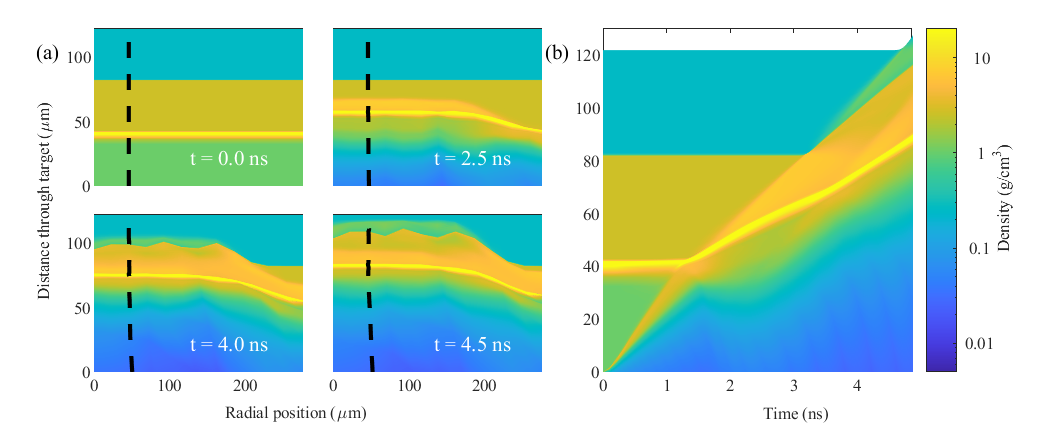
\includegraphics[width=1\textwidth]{figures/Experiment/H2DPlot.eps}% Here is how to import EPS art
\caption{\label{fig:H2DPlot} A two-dimensional h2D simulation of the setup using a simple four-layer target (ablator, gold, quartz and foam without the step structure), for a laser intensity of \num{1e14} \unit{\W\per\centi\meter\squared}. (a) shows four snapshots of the 2D simulation at the indicated times, while (b) shows the shock propagation of through the target as a function of time for a given radial position, represented by the black dashed lines in (a). It can be seen that for the later two times, the black dashed line is noticeably curved. This is because the lagrangian mesh moves as the simulation occurs, and thus the mesh points (where the simulation parameters are returned) do not have fixed radii. This small amount of curvature does not significantly affect the results - particularly as it is only seen in the ablated material significant behind the shock.}
\end{figure}

Figure \ref{fig:H2DPressure} shows how the pressure just behind the shock front in this simulation varies across the radius of the target. It is clear from the figure that, while the pressure reduces towards the edge of the target, over the central region the shock pressure is relatively planar in both the quartz and the foam. Meanwhile, Figure \ref{fig:H2DTiming} displays the shock breakout times from the gold, quartz and foam layers. This again indicates that the shock is planar over the central region of the laser spot.

\begin{figure}[hbt!]
\centering
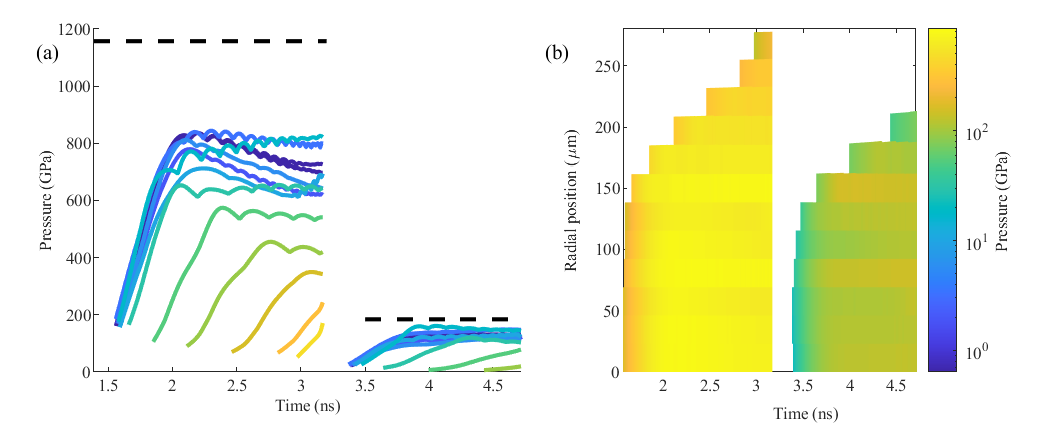
\includegraphics[width=1\textwidth]{figures/Experiment/H2DPressure.eps}% Here is how to import EPS art
\caption{\label{fig:H2DPressure} Plots showing the shock pressure in the simulation displayed in Figure \ref{fig:H2DPlot} as a function of both time and radial position. In (a), the different lines represent the different radial positions, with the colour transitioning from dark blue through to yellow (i.e. up the colour bar in Figure \ref{fig:H2DPlot}) as the radius moves further away from the center of the target. It can be seen here that the pressure is relatively uniform over the central regions, but drops off towards the edge. The dashed line represents the average shock pressure obtained in both materials in the 1D simulation. It is clear that this is significantly higher, but the difference appears to depend on simulation parameters (such as resolution) and was not observed in the other 2D codes. (b) represents the same data, but here the pressure is represnted by the colour on the 2D plot of position vs time. On both plots, the shock front pressure is only recorded when the shock front can be automatically identified in the simulation, and thus there are blank regions when the shock crosses material interfaces and the shock front cannot be clearly identified.}
\end{figure}

\begin{figure}[hbt!]
\centering
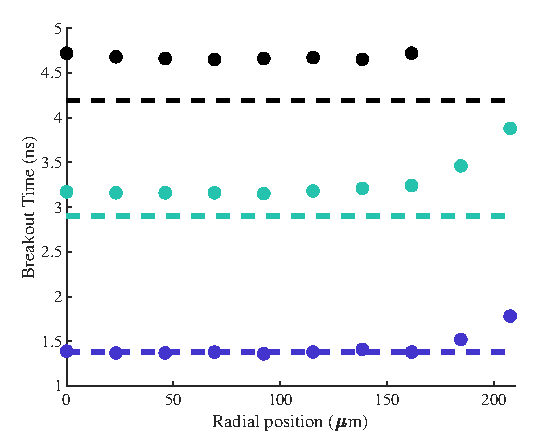
\includegraphics[width=0.6\textwidth]{figures/Experiment/H2DTiming.eps}% Here is how to import EPS art
\caption{\label{fig:H2DTiming} Shock breakout times from the gold (blue points), quartz (teal points) and foam (black points) as a function of radial position in the target. It can be seen that the breakout time is roughly steady over a radius of 150 \unit{\micro\meter}, and then increases towards the edge of the laser pulse. The dashed lines represent the breakout times obtained from the 1D Hyades simulation. While there is good agreement for the gold breakout, the 2D simulation returns a later breakout from the quartz and the foam, suggesting a slower and weaker shock. This is not observed in the other 2D simulations.  }
\end{figure}

Both Figure \ref{fig:H2DPressure} (a) and Figure \ref{fig:H2DTiming} also compare these results to the 1D Hyades simulation shown in Figure \ref{fig:PreExpHydro}. It can be seen that the timing agreement is reasonably close, but there is a small increase in the shock transit time in both the quartz and the foam. This increase in transit time is due to a decreased shock velocity, which in turn indicates a lower shock pressure as seen in Figure \ref{fig:H2DPressure}. While the change in shock transit is relatively small, the corresponding impact on the pressure is relatively significant. Interestingly, as can be seen in the post-experiment simulations, such an effect was not observed to the same extent in the simulations performed in other 2D codes. This effect (particularly the pressure) was found to vary with the resolution of the simulations, suggesting it had not fully converged; unfortunately it was not possible (due to persistent issues with mesh tangling and crashing) to increase the resolution of the simulation to a point where the results converged. As such, while the h2D simulation was useful for confirming the shock planarity and expected behaviour in 2D, it was decided that the results should not be relied on for the precise shock timings/pressures, and the other codes (such as Multi and FLASH) were used for the post-experiment 2D simulations.


%were also performed in a variety of codes, to check that the shock was relatively consistent across the shock diameter. Simulations were performed in h2D (the 2D version of Hyades) which showed that the shock behaviour was largely similar to that seen in Hyades. The shock was planar over most of the 400\unit{\micro\meter} imaged region, and the transit time was only slightly reduced compared to the 1D simulations. Piotr R\k{a}czka also performed a 2D Flash simulation which included the target step (as h2D was a lagrangian code, issues with mesh tangling prevented such a simulation from being performed) and showed that this did not significantly affect the shock propagation.

\section{Conducting the experiment}

The experiment was performed over a five and a half week period. Roughly two and a half weeks of this were setup, with a further three weeks of experimental shots. A series of images showing the experimental setup can be seen in Appendix \ref{app:2-experimentphotos}.

Throughout the run a number of changes were required from the original setup and experimental plan. These are outlined and explained in the following sections.

\subsection{Changes from planned target} \label{Target issues}
The actual targets that were delivered for the experiment differed slightly from the planned targets. This was due to challenges in fabricating the targets, as well as one of the suppliers failing to deliver a shipment of quartz (which also limited the number of available targets).
\begin{itemize}
    \item \textbf{Different target dimensions}: the delivered quartz was thicker than expected, which led to the quartz layer in each target being $\sim$ 50 \unit{\micro\meter} thick (rather than the planned 40 \unit{\micro\meter}). The foam thickness also varied, and was frequently significantly larger than the planned 40 \unit{\micro\meter}.
    \item \textbf{Fewer targets with an AR coating}: the reduced quantity of quartz meant that some targets did not have the planned anti-reflection coating. Fortunately, this did not seem to have a significant effect.
    \item \textbf{Delamination in some targets}: in a small number of early targets, the ablator/gold delaminated from the quartz, and had to be glued back on. The glue layer prevented an accurate timing measurement in the quartz and meant that the target could not be used for impedance matching; however, they were shot as test/setup targets. These later became important in understanding some features of the results (see Section \ref{Glue targets}).
\end{itemize}

\subsection{Poor VISAR illumination and subsequent changes to optical setup}

Once setup was complete and shots started, it became apparent that the probe laser was only illuminating a small section of the imaged region. This prevented sufficient VISAR data from being collected. This was due to the fact that the probe laser travelled through the optical relay before reaching the target, which demagnified it and brought the laser to focus at the target position, as seen in Figure \ref{fig:Full experiment schematic}. 

An initial solution was to place a 700 \unit{\milli\meter} focal length lens between the laser and the VISAR beamsplitter; this would mean the laser was not collimated when entering the relay, and so would not be perfectly focussed by the objective lens. This did not sufficiently improve the problem. As such, a modified setup was designed which would solve the problem while requiring minimal changes to the optical relay (which at this point was already setup). In the new setup, the first mirror after the objective lens was replaced with a beamsplitter, and the probe laser was injected through this beamsplitter rather than after the VISARs. This meant the probe laser bypassed the relay, and only the objective lens was shared. A lens was placed in the probe laser beampath prior to this beamsplitter to form a lens pair with the objective lens; this meant that the probe laser would be collimated by the objective lens, and thus collimated when it reached the target \footnote{While this was initially the case, extra mirrors were later added to the setup to give additional control one the probe laser position. Spatial constraints meant these mirrors had to be added between the lenses, which increased the P1-L1 distance from the intended 550mm to 875mm. This meant that the beam was no longer perfectly collimated. However, burn paper tests showed that the spot size at the target position was still sufficient, and the illumination remained uniform. Simulation of this setup with the ray tracing code suggested the spot size was around 1 mm in diameter.}. A simple schematic showing this new setup can be seen in Figure \ref{fig:Full experiment schematic with new laser setup}, with a schematic showing the spatial arrangement shown in Figure \ref{fig:Full setup}. A scale 3D CAD model and engineering drawings with measurements of this setup are provided in Appendix \ref{app:2-experimentphotos}.

\begin{figure}
\begin{centering}
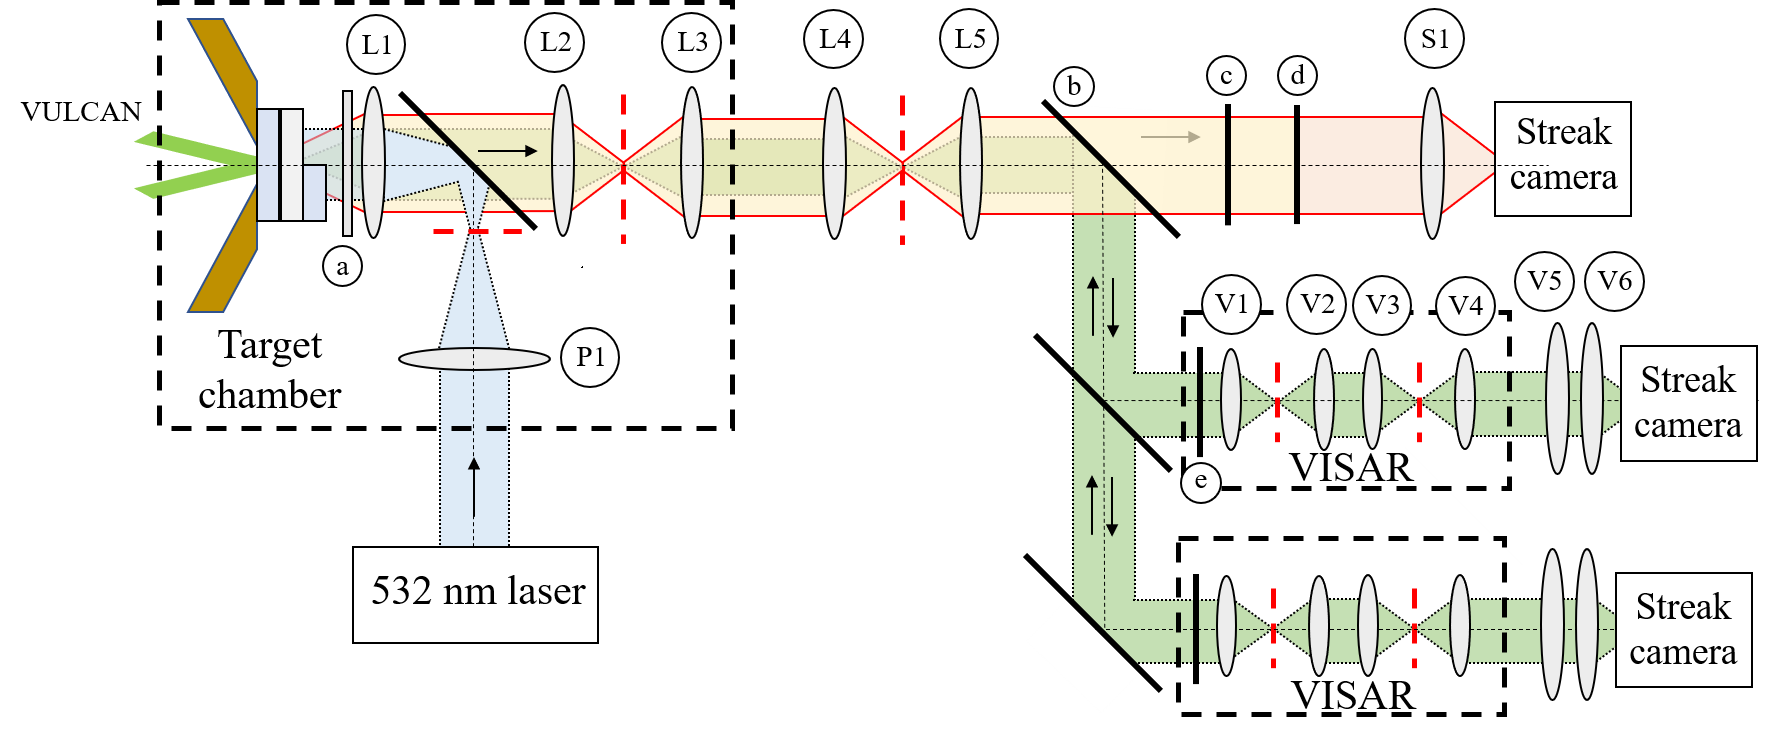
\includegraphics[width=1.0\textwidth]{figures/Experiment/Full experiment schematic new laser injection.png}% Here is how to import EPS art
\caption{\label{fig:Full experiment schematic with new laser setup} The full schematic, with the new probe laser injection. The probe laser is displayed in blue to differentiate the beampath from the reflected probe light shown in green, but both have the same 532 nm frequency. The labels are unchanged from Figure \ref{fig:Full experiment schematic}, except for a new 400 mm lens P1. This forms a lens pair with the objective lens L1; the beam passes through P1 and is focussed at the focal point of L1, so that L1 collimates the beam before it reaches the target. The incoming laser is then scattered from the target, and the objective lens is thus still considered to be collimating the reflected light. The only other changes from the original setup are the addition of a beamsplitter between L1 and L2 (replacing a mirror in the previous setup), and the replacement of the beamsplitter prior to the bottom VISAR with a mirror.}
\end{centering}
\end{figure}

\begin{figure}
\begin{centering}
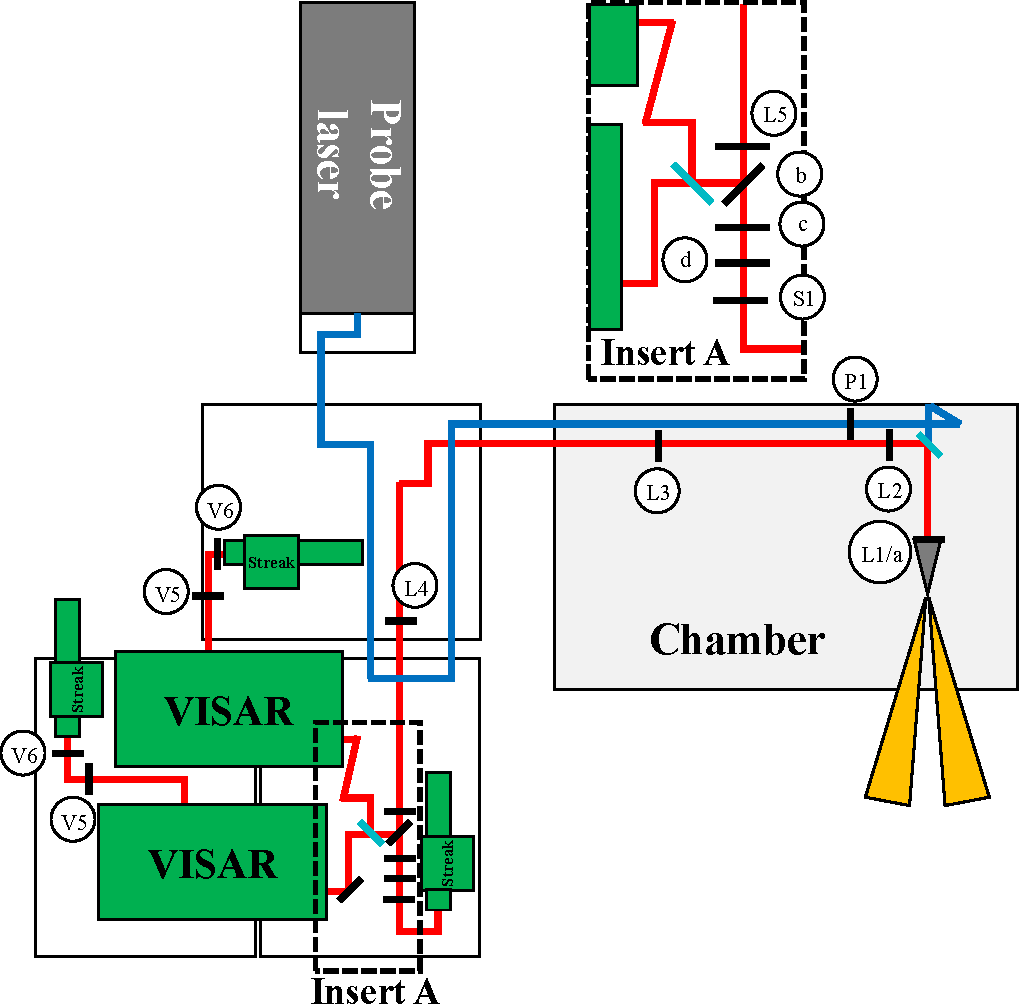
\includegraphics[width=1.0\textwidth]{figures/Experiment/FinalSetup.pdf}% Here is how to import EPS art
\caption{\label{fig:Full setup} The updated spatial arrangement. The labels are as in previous figures. The main changes are the new beampath route for the probe laser, which leads to a beamsplitter between L1 and L2 (previously a mirror), and the removal of the beamsplitter before the second VISAR (replaced with a mirror).}
\end{centering}
\end{figure}

This setup significantly improved the illumination, as shown in Figure \ref{fig:VISAR before and after}. The downside of this approach was that the beamsplitter in the relay would reduce the intensity of the captured emission (both the VISAR signal and the self-emission) by half (although the second VISAR beamsplitter could be replaced with a mirror, which compensated for the signal loss on one of the VISARs). This was a necessary sacrifice though, as without this change the illumination was not sufficient for the VISAR to be used.

\begin{figure}
\begin{centering}
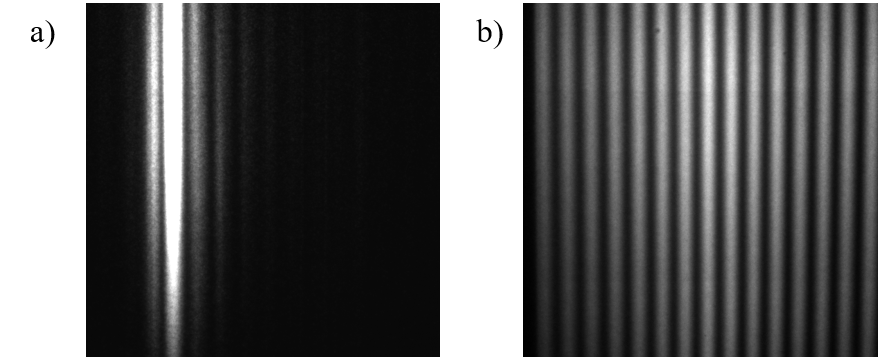
\includegraphics[width=0.8\textwidth]{figures/Experiment/VISAR before and after.png}% Here is how to import EPS art
\caption{\label{fig:VISAR before and after} Images taken in focus mode on the VISAR streak camera from a piece of quartz a) using the original setup and b) using the updated setup. The quartz sample is stationary, and the camera used in focus mode so the signal at a single time across two spatial dimensions is recorded; uniform fringes are expected across the whole image. It is clear that in (a) only part of the sample is well-illuminated, whereas the new setup well illuminates the full imaged region. The signal strength was also better using the new setup; (a) is only brighter due to different filtering.}
\end{centering}
\end{figure}

\subsection{Later than expected shock breakout times}

It was noted mid-experimental run that the shock breakout times being measured for a given intensity were significantly longer than those predicted by simulations. This meant that the VULCAN drive beam was frequently ending prior to shock breakout - contrary to the experimental plan, where the drive beam would be kept on until shock breakout to ensure a sustained shock. Additional simulations were therefore performed mid-run to determine the expected impact of the drive laser pulse ending before shock breakout time. It was found that in fact this did not lead to substantial differences in shock behaviour, and thus this was not a major cause for concern.

There was also concern that this could be due to a lower than expected laser intensity. However, the pulse time and pulse energy were directly measured for each shot using the diagnostics, and the laser spot diameter could easily be estimated from the pinhole image (the complete post-experiment analysis of this is given in Section \ref{Other diagnostic analysis}). This suggested that the intensity was as expected, and not responsible for the issue.

\subsection{Signal strength issues}

Throughout the experiment, both diagnostics suffered from a lack of signal strength. Some of this could be explained by the streak cameras. Three were used in this experiment; two high dynamic range Hamamatsu C7700 cameras were used for the VISARs, while a Hamamatsu C5680 was used for the streaked optical pyrometer. The older C5680 was expected to be less sensitive, and this was used for the SOP accordingly (as the VISAR was the more important diagnostic). This camera struggled for signal throughout. One of the VISARs also consistently recorded low signals compared to the other; it was later realised that this camera had an S1 streak tube as opposed to the S20 used in the other. The S1 tube (which was also present in the SOP streak) is around two orders of magnitude less sensitive to 532 \unit{\nano\meter} light.

The signal strength for both VISARs was also heavily influence by the probe laser. This laser was relatively high power, and significant ND filters were needed to prevent it damaging the optics in the optical chain. However, the long optical relay likely resulted in some decrease in signal strength. There were also significant operational issues with the probe laser. It frequently did not seed, resulting in the pulse being significantly weaker, and being emitted at a different time. This would occur on shots, where the low strength and change in time (relative to the VULCAN pulse) would prevent useful data from being collected. After attempting a number of fixes, the facility staff eventually replaced the seed laser within the unit with one from a different laser. This improved the situation and allowed the experiment to continue, but the timing and pulse intensity continued to vary drastically from shot to shot.



\chapter{\label{ch-experimentAnalysis} Measuring the TMPTA principal Hugoniot: analysis and interpretation}

\minitoc

\section{Introduction}

This chapter will outline the steps taken to analyse the data from Chapter \ref{ch-experiment}. The results will then be discussed and compared with simulation, and a few unexpected features in the data investigated. 

In Section \ref{VISAR analysis}, the analysis of the VISAR data will be discussed, showing how the streak images can be used to calculate the shock state achieved in the foam on each shot. Section \ref{SOP analysis} focuses on the SOP data, describing how this was used to calculate the shock temperature, and how SOP timing data could be compared to that obtained from the VISAR. Section \ref{Other diagnostic analysis} then looks at the information that could be obtained using the fiducial, pinhole camera, and photodiode traces of the laser pulse. The data analysis then concludes with Section \ref{Data choices}, which broadly describes how decisions were made regarding the final data set.

The main results are then discussed in Section \ref{Experiment Results}, where they are compared to both theoretical models and data from previous experiments on similar materials. Comparison with post-experiment simulations is then presented in Section \ref{Post shock simulations}. Section \ref{Weak quartz shock} then describes how a certain feature of the data - a weaker than expected shock in the quartz - was investigated, and explores a potential explanation for this. Finally, Section \ref{Suggested Improvements} discusses suggested improvements that could be made were such an experiment to be performed again.

The structure used here has been chosen to aid explanation of the results, and roughly follows how it was actually performed. However, the analysis was in reality an iterative process; early stages were refined and revised later on, and early results from the preliminary analysis meant that this was performed with some knowledge of the final data set. A basic confidence ranking had to be performed early on to obtain preliminary results and spot trends in the data, and this was then updated as understanding and interpretation of the data set improved. In recognition of this, the results from each stage of the described analysis will be included in that section, although these will not be discussed in detail until Section \ref{Experiment Results}. The data set used in these results is the data set selected in Section \ref{Data choices} (highlighting the iterative nature of this analysis!).

Throughout this chapter, experimental data is displayed to aid understanding of the analysis. For consistency, wherever possible data from the same shot has been used, but this was not always possible. Shot 38 is used for the general VISAR and SOP analysis, as this shot contained the clearest data. However, it did not have a fiducial present, which meant that the ablator/gold transit times could not be determined - the simulations therefore focus instead on an alternative shot, Shot 47. Data from other shots are sometimes used where necessary to best show a particular feature of behaviour - these shots are identified for transparency.

%I performed the work described in this chapter, and wrote the code in which the analysis was performed. I also performed a large amount of the simulation work, and interpreted the data. I have included some work performed by the other experimental collaborators, and have indicated where this arose. This was predominantly in the analysis of the curved VISAR data (where I performed the analysis based on code written by Daniel Eakins), and in the simulation work, where Multi and some of the Helios simulations were performed by Paul Neumayer and Artem Martynenko, and the Flash simulations were performed by Piotr R\k{a}czka.

\section{Analysis of VISAR data} \label{VISAR analysis}
%\subsection{Collected data for a typical shot}

%The data collected for a typical shot is consisted of:
%\begin{itemize}
%\item Photos of the target (taken by target fabrication)
%\item Measurements of the target dimensions (performed by target fabrication)
%\item Measurements of the energy of each beam (from the on-shot calorimetry)
%\item Traces of the pulse profile of the beams (taken from photodiodes viewing parasitic signal from a lossy-mirror)
%\item Images from each VISAR streak camera (one from each, two in total)
%\item Image from the SOP streak camera (one - containing fiducial signal from start of beam)
%\end{itemize}

\subsection{Identifying shock velocities from raw VISAR data}

In the VISAR streak images, the x-axis position is a spatial dimension, and the image contains two distinct halves - one corresponding to the quartz, and the other to the foam. The y-direction represents time, with later times at the bottom of the image. A labelled example can be seen in Figure \ref{fig:VISARImage}. Three `transitions' can be identified in the image. Firstly, shock entry into the quartz can be identified by a sudden change in signal intensity on the quartz half of the image. Secondly, shock breakout from the quartz rear-surface can be identified by fringe extinction on this half. This also corresponds to the shock entering the foam (although as the foam is opaque to the probe laser, no change is seen in the foam signal at this point). Finally, shock breakout in the foam could also be identified by fringe extinction, but on the other half of the image.

\begin{figure} [h]
\begin{centering}
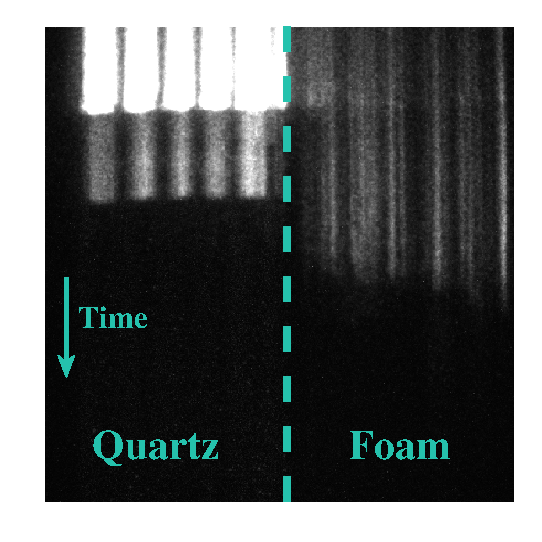
\includegraphics[width=0.5\textwidth]{figures/Experiment/VISARImage.eps}% Here is how to import EPS art
\caption{\label{fig:VISARImage} A raw VISAR streak image for shot 38, labelled to indicate the quartz and foam signals. Three clear changes can be observed; a change in fringe intensity in the quartz (corresponding to the shock entering the quartz from the gold), fringe extinction in the quartz (shock breakout from the quartz), and fringe extinction in the foam (shock breakout from the foam). }
\end{centering}
\end{figure}

Both VISAR images were viewed side by side, and the contrast adjusted to aid identification of these changes. On each image, where possible, the three times were selected. The selections used for an example shot are displayed in Figure \ref{fig:VISAR ROI}. As the change in signal was not always instantaneous, a `region of interest' (ROI) was selected to cover the full range over which the transition most likely occurred. 

\begin{figure} [h]
\begin{centering}
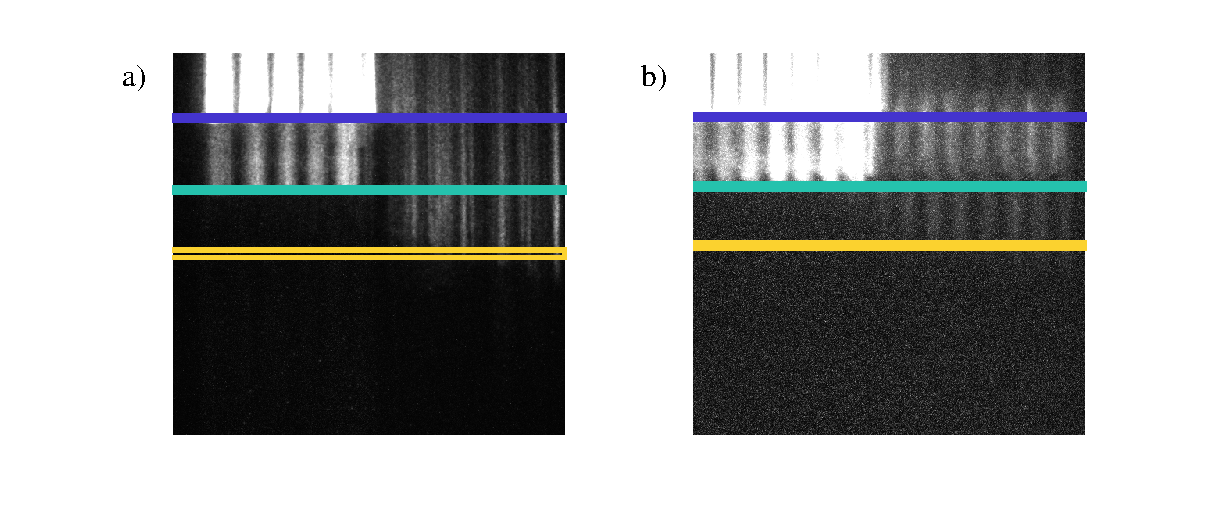
\includegraphics[width=1.0\textwidth]{figures/Experiment/VISARROI.eps}% Here is how to import EPS art
\caption{\label{fig:VISAR ROI} VISAR images from the two VISARs for shot 38. The selected regions where the shock transitions are believed to be confirmed are shown. The blue region corresponds to shock entry into the quartz, while the teal region corresponds to shock breakout from the quartz and the yellow corresponds to shock entry into the foam. The edge of image (a) appears to show some curvature; this is expected based on the simulations due to the size of the VULCAN laser spot. The region was chosen to capture the transition at the center, where the shock seems to be more planar.}
\end{centering}
\end{figure}

The streak time was and used to convert the pixels (in the y-direction) to time. The ROI's were thus converted from a pixel range into a time (the mean position of the window) with associated uncertainty (the width of the window). The finite slit width of the camera also introduced a minimum possible time resolution (which was used for the uncertainty if the ROI width was less than this value). The shock transit times through both quartz and foam were then calculated, as the differences between these three transitions.

The two VISARs, when both operating well, gave independent measurements of the same behaviour. In many cases, each transit time could only be confidently identified from one of the two VISARs - in such cases, only the transit times from a single image were used. However, in cases where both VISARs returned good data, the calculated transit times from the two diagnostics were combined. Since the value from both should be consistent, having two measures allowed the error to be reduced. The 'average' measurement range was taken as the region in which the two separate measurements overlapped.

Finally, the thickness of the quartz and foam layers (with estimated uncertainties) were then used to calculate the average shock velocity in each material. The shock velocity calculated for a single shot using the independent time measurements from each VISAR, along with that calculated from the combined time measurements, are shown in Figure \ref{fig:VISAR Timing}.

\begin{figure} [h]
\begin{centering}
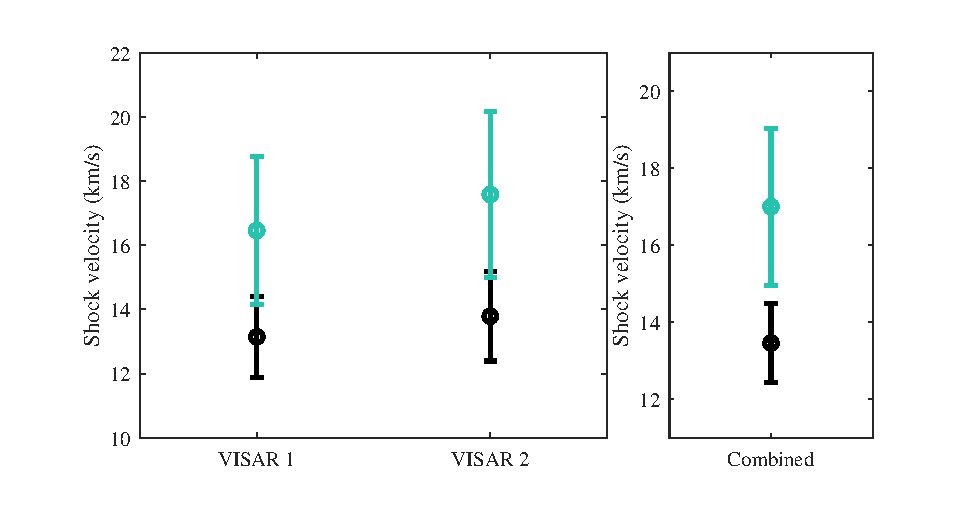
\includegraphics[width=1.0\textwidth]{figures/Experiment/VISARTiming.eps}% Here is how to import EPS art
\caption{\label{fig:VISAR Timing} Calculated shock velocities in the quartz (black) and the foam (teal)  for shot 38, using the shock timings obtained from the VISAR images in Figure \ref{fig:VISAR ROI}. In this shot, all three timings can be identified from both VISARs. The shock velocities corresponding to the timing data from each of the two VISARs independently is displayed, along with the shock velocity calculated from the `combined' timings. The combined measurement uses both sets of VISAR measurements to reduce the error, giving a `combined' set of possible timings that is compatible with the range measured by each VISAR.}
\end{centering}
\end{figure}

%An attempt was made at this point to identify the same three transitions from the SOP data, to provide another measure of these shock transit times. However, this turned out not to be possible - there was no clear change in the SOP data correlating to the shock breakout from the quartz, which prevented either shock breakout time from being calculated. It was also found that the start of the foam self-emission occurred before the shock breakout in the VISAR images (likely indicating some transparency of the foam to these self-emitted frequencies).


\subsection{Impedance matching calculation} \label{IM calc}
The impedance matching calculation was then performed to calculate the foam shock state from the two shock velocity measurements. The principles behind this calculation is described in Sections \ref{IMTheory} and \ref{IMTheoryMeasurements}, where in this case the quartz is the reference material (for which the Hugoniot and release isentrope are known) and the foam is the material of study.

An initial faster but less accurate impedance matching calculation was performed to assess the data (and to provide a sanity check on the more accurate, but more complicated, subsequent calculation). This used a common assumption that the quartz release isentrope can be approximated by reflecting the quartz hugoniot around the quartz shock state. This is a reasonably accurate approximation at low pressures, but can introduce errors as the pressure is increased \cite{Forbes2012}. In this calculation, the quartz Hugoniot described in \cite{Knudson2009} was used, with a functional form of 
\begin{equation} \label{eqn:Old Hugoniot} U_s = a + b u_p - c u_p \exp{-d u_p}, \end{equation}
with coefficients of $a = 6.26 \pm 0.35$ \unit{\kilo\meter\per\second}, $b = -1.20 \mp 0.02$ , $c = 2.56 \mp 0.15$, and $d = 0.37 \pm 0.02$ $(\unit{\kilo\meter\per\second})^{-1}$. Then, as described in Section \ref{IMTheoryMeasurements}, the measured shock velocities were used to produce the quartz and foam Rayleigh lines. The intercept of the quartz Rayleigh line with quartz Hugoniot was used to determine the quartz shock state. The quartz Hugoniot was then reflected about this state, and the intercept of this approximate release isentrope with the foam Rayleigh line allowed the foam shock state to be calculated. This calculation was performed for each shot, and the preliminary results indicated that there was indeed a trend in the data and thus the more complicated analysis should be conducted.

%A common approximation in impedance matching calculations is not to calculate the release isentrope, but instead to reflect the hugoniot of the reference material (for this experiment, quartz) around the reference material (quartz) shock state. For low pressures this is reasonably accurate, but it can introduce errors as the pressure is increased. An initial calculation was performed using this approach to produce a first estimate of the results, and to provide a sanity check on the results of the more complicated (but more complete) approach. In this calculation, the Hugoniot described in \cite{Knudson2009} was used: \begin{equation} \label{eqn:Hugoniot} U_s = \sum_{n=0}^3 a_n u_p^n \;, \end{equation} with coefficients in Table \ref{tab:HugoniotCoeffs} \cite{Knudson2013} - a cubic fit to experimental data from \cite{Knudson2009} The intercept of this Hugoniot with the quartz Rayleigh line,  $P = \rho_0^{quartz} U_s^{quartz} u_p$, where $P$ is Pressure, $u_p$ is particle velocity, and $U_s^{quartz}$ is the measured quartz shock velocity, was found. This intercept provided ($P^{quartz}, u_p^{quartz}$), the quartz shock state. The Hugoniot was then reflected around this point to approximate the release isentrope. The intercept of this reflected Hugoniot with the foam Rayleigh line, $P = \rho_0^{foam} U_s^{foam} u_p$, was then found, which defined the foam shock state ($P^{foam}, u_p^{foam}$). This was performed for each shot.

\begin{table}%The best place to locate the table environment is directly after its first reference in text
\centering
\caption{\label{tab:HugoniotCoeffs}%
Coefficients for the quartz Hugoniot in equation \ref{eqn:Hugoniot}, reproduced from \cite{Knudson2013}.
}
\begin{tabular}{lccr}
\hline\hline
\textrm{$a_0$ \si[per-mode=symbol]{(km/s)}}&
\textrm{$a_1$}&
\textrm{$a_2$ \si[per-mode=symbol]{\kilo\meter\per\second} }&
\textrm{$a_3$ \si[per-mode=symbol]{(km/s)^{-2}} } \\
\hline
1.754 & \num{1.862} & \num{-3.364E-2} & \num{5.666E-4}\\
\hline\hline
\end{tabular}
\end{table}

The more accurate calculation used a full and complete calculation of the release isentrope. For this version of the impedance matching calculation a slightly different functional form for the Hugoniot was used \cite{Knudson2013} - a cubic fit to the same data as used previously \cite{Knudson2009}. The new Hugoniot was described by \begin{equation} \label{eqn:Hugoniot} U_s = \sum_{n=0}^3 a_n u_p^n \;, \end{equation} with coefficients in Table \ref{tab:HugoniotCoeffs}. This newer form was used to facilitate the use of Monte Carlo error analysis (described in Section \ref{MC error}). The release isentrope was then accurately calculated according to the relevant quartz shock state. This was done largely according to the method outlined by Knudson and Desjarlais \cite{Knudson2013}, but with a few small differences. 

In their paper, Knudson and Desjarlais model the isentrope using a new `linear-reference' Mie-Gruneison model. The key departure of this model from other approaches is the use of a variable Gr{\"u}neisen parameter. They compare the new model to the previous standard - a conventional Mie-Gruneison model with a fixed Gr{\"u}neisen parameter of $\Gamma = 0.64$ - and found that the new model led to reduced errors. However, the range of pressures over which this model is valid does not extend across those achieved in this experiment, and the model  returned implausible results for some of these values. As such, the conventional Mie-Gruneison model, with a fixed Gr{\"u}neisen parameter of $\Gamma = 0.64$, was used. This value of the Gr{\"u}neisen parameter was calculated from a range of EOS models \cite{Hicks2008}, and is in good agreement with that derived \cite{Hicks2008} from experiments \cite{Hicks2005, Trunin1994}. Other than this change to the Gruneison parameter, the method for calculating the release isentrope for a given quartz shock state was as Knudson and Desjarlais described \cite{Knudson2013}.

The impedance matching calculation was therefore conducted as in the previous method, with this more accurate model for the quartz isentrope used, and the foam shock ( $u_p^{foam}, P^{foam}$) state was determined from the intercept of this curve with the foam Rayleigh line. A graphical representation of this for the experimental data from Shot 38 is shown in Figure \ref{fig:Impedance Match}. This calculation was performed for all shots. A comparison with the previous method, using the reflected Hugoniot as the isentrope, found the difference to be essentially negligible; this suggests the isentrope is comparable to the reflected Hugoniot in this regime, and provided a sanity check that the release isentrope had been calculated correctly.

%The calculation follows that described for the reflected-Hugoniot model, except that once the quartz shock state ($P^{quartz}, u_p^{quartz}$) has been found, the associated isentrope for that state is calculated following the method described in appendix. This is then used in place of the reflected Hugoniot. Once this had been performed for all shots, the results of this calculation were compared to the reflected hugoniot ones, and the difference was found to be negligible. A graphical representation of this imedance matching calculation is shown in Figure \ref{fig:Impedance Match}.

\begin{figure} [h]
\begin{centering}
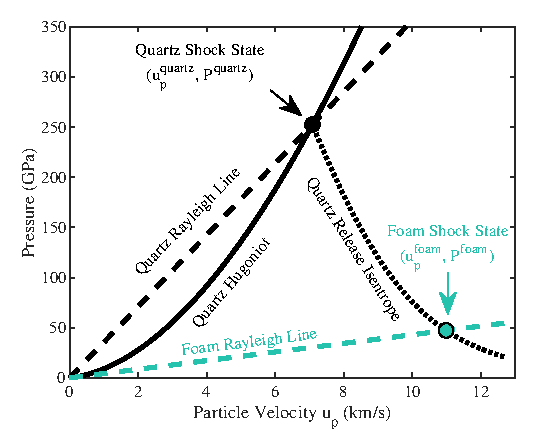
\includegraphics[width=0.6\textwidth]{figures/Experiment/ImpedanceMatch.eps}% Here is how to import EPS art
\caption{\label{fig:Impedance Match} The impedance matching calculation for the shock velocities obtained from shot 38. The intercept of the quartz Rayleigh line and the quartz Hugoniot defines the quartz shock state. The release isentrope for this shock state is then calculated, and the intercept of this curve with the foam Rayleigh line describes the foam shock state.}
\end{centering}
\end{figure}

The resulting foam shock states for the final data set are displayed in Figure \ref{fig:Hugoniot}, where they are compared to theoretical models. These results will be discussed in Section \ref{Experiment Results}. The error bars are explained in Section \ref{MC error}.

\begin{figure} [h]
\begin{centering}
\includegraphics[width=0.6\textwidth]{figures/Experiment/Hugoniot.eps}% Here is how to import EPS art
\caption{\label{fig:Hugoniot} The foam hugoniot data calculated from the impedance matching calculation, compared to hugoniots generated from theoretical equation of state models.}
\end{centering}
\end{figure}


\subsection{Uncertainty quantification - Monte Carlo analysis} \label{MC error}

Uncertainty quantification for the shock variables obtained using the impedance matching calculation was performed using a Monte Carlo approach \cite{Root2010}. This technique allowed the experimental uncertainty to be propagated through the complex IM calculation, while also including uncertainty contributions from the quartz hugoniot fit and foam initial density. This section is accompanied by a flow chart in Figure \ref{fig:MC Flow Chart} which shows the different steps of the calculation for the shot considered in the previous sections, with the relevant distributions and example MC samples. Uncertainty quantification in this way has previously been performed on other similar experiments \cite{Knudson2013, Root2010, Root2013, McCoy2016}.

%My initial solution to this problem was to perform each calculation three times for a single shot. Consider the IM calculation as a black box, which takes inputs (shock velocities) and returns outputs (shock pressures, particle velocities etc.). If we take an input of $A \pm B$, the calculation was performed for A, A + B, and A - B. This would return answers of C, D, and E - where C is the 'value' we would then use, and D and E are the ranges of our uncertainties. This approach worked, but lacked elegance. It was difficult to include Hugoniot error, and it also required careful thought to ensure the right 'sets' of inputs were included to make sure the uncertainties summed in the right way. This approach also had statistical flaws - I was finding max errors by assuming that each input had it's maximal error at the same time (a worst-case scenario), but this is more pessimistic than standard error propogation formulas, and thus led to larger errors.

The calculation begins with the measured shock velocities for the quartz and foam for a particular shot. These are of form $U_{shock} \pm \epsilon$; a quoted value $U_{shock}$, with an experimentally measured error that is symmetric around this value $\epsilon$. A normal distribution is then produced for each of the two shock velocities; this has a mean at the value $U_{shock}$, and a standard deviation of $\epsilon$. A similar distribution is produced for the foam initial density.

These distributions were then used to perform 10,000 Monte Carlo iterations of the impedance matching calculation for each shot. For each iteration, a sample is randomly generated for each shock velocity and the foam density according to the relevant distribution. Samples are also generated for each of the four Hugoniot fit parameters, according to the covariance matrix covariance matrix\footnote{The printed matrix is that provided by \cite{Knudson2013}, but actually attempting to use this to generate the parameters returned an error due to the matrix not being positive definite. To resolve this, a small correction was added, $C + \num{1e-10}\cdot I$ was required, where $I$ is the identity matrix \cite{Holton2003}.} provided in \cite{Knudson2013},
\[C = 
\begin{bmatrix}
\num{2.097e-2} & \num{-6.159e-3} & \num{5.566e-4} & \num{-1.572 e-5}\\
\num{-6.159e-3} & \num{1.877e-3} & \num{-1.742e-4} & \num{5.017e-6}\\
\num{5.566e-4} & \num{-1.742e-4} & \num{1.650e-5} & \num{-4.834e-7}\\
\num{-1.572 e-5} & \num{5.017e-6} & \num{-4.834e-7} & \num{1.438e-8}\\
\end{bmatrix}. 	
\]

The impedance matching calculation was then performed, as described in Section \ref{IM calc}, using these randomly sampled values. The 10,000 iterations produced 10,000 different estimates of the quartz and foam shock states, providing distributions for each of the relevant shock variables. The standard deviations $\sigma$ of these distributions were then calculated, and used to define the uncertainty range of these values.


%\begin{table}%The best place to locate the table environment is directly after its first reference in text
%\caption{\label{tab:HugoniotCovariance}%
%Coefficients for the quartz Hugoniot in equation \ref{eqn:Hugoniot}, reproduced from \cite{Knudson2013}.
%}

%\begin{tabular}{lccccccccr}
%\hline\hline
%\begin{tabular}{@{}c@{}}$\sigma_{a_0}^2$ \\ $(\times 10^{-2})$\end{tabular}
%\begin{tabular}{@{}c@{}}$\sigma_{a_0}\sigma_{a_1}$ \\ $(\times 10^{-3})$\end{tabular}
%\begin{tabular}{@{}c@{}}$\sigma_{a_0}\sigma_{a_2}$ \\ $(\times 10^{-4})$\end{tabular}
%\begin{tabular}{@{}c@{}}$\sigma_{a_0}\sigma_{a_3}$ \\ $(\times 10^{-5})$\end{tabular}
%\begin{tabular}{@{}c@{}}$\sigma_{a_1}^2$ \\ $(\times 10^{-3})$\end{tabular}
%\begin{tabular}{@{}c@{}}$\sigma_{a_1}\sigma_{a_2}$ \\ $(\times 10^{-4})$\end{tabular}
%\begin{tabular}{@{}c@{}}$\sigma_{a_1}\sigma_{a_3}$ \\ $(\times 10^{-6})$\end{tabular}
%\begin{tabular}{@{}c@{}}$\sigma_{a_2}^2$ \\ $(\times 10^{-5})$\end{tabular}
%\begin{tabular}{@{}c@{}}$\sigma_{a_2}\sigma_{a_3}$ \\ $(\times 10^{-7})$\end{tabular}
%\begin{tabular}{@{}c@{}}$\sigma_{a_3}^2$ \\ $(\times 10^{-8})$\end{tabular} \\
%\hline
%2.097 & -6.159 & 5.566 & -1.572 & 1.877 & -1.742 & 5.017 & 1.650 & -4.834 & 1.438\\
%\hline\hline
%\end{tabular}
%\end{table}


10,000 Monte Carlo iterations were then performed. For each iteration, a random sample was taken from each distribution. The impedance matching calculation was then performed using this random set of values. Overall, this produced 10,000 different calculated quartz and foam shock states, giving distributions of each output value (i.e. quartz/foam pressures, particle velocities etc.). The uncertainty of each of these parameters was taken as the standard deviation of the corresponding distribution.

The mean of the MC distribution of a particular value does not always equal the `exact' value obtained if the IM calculation is performed without considering uncertainty (i.e. if no MC sampling is performed, and thus for all shock velocities $U_{shock} \pm \epsilon$ the values of $U_{shock}$ are used, along with the exact Hugoniot fit parameters quoted in Table \ref{tab:HugoniotCoeffs}). This was most noticeable for the shock pressure, where there is a small amount of skew in the distribution\footnote{Skew in the MC distributions of such an experiment was also previously noted in \cite{Root2013}.} (the particle velocity distributions are effectively normal). This effect arises from a non-linearity in the calculation. Consider a shock velocity $U_{shock}$ and associated pressure $P$. A small positive increase in $U_{shock}$ results in a larger change in $P$ than a small decrease in $U_{shock}$, leading to a distribution mean that is skewed towards higher values.

The most obvious way to present the results of this calculation would be to quote each shock variable as the MC mean plus/minus the standard deviation. This could lead to confusion; for instance, the quartz shock state would then be quoted as $\bar{u_p}^{quartz} \pm \sigma_{u_p^{quartz}}$ and $\bar{P}^{quartz} \pm \sigma_{P_{quartz}}$ (where a variable with a bar is used to indicate the MC distribution mean), but the state ($\bar{u_p}^{quartz}, \bar{P}^{quartz}$) would not actually be a valid state on the quartz Hugoniot described by Equation \ref{eqn:Hugoniot}. To avoid this, the shock variables are instead quoted as the `exact' values - those obtained if the IM calculation is done without random sampling of any of the variables. These values are quoted with asymmetric error to describe the same uncertainty range as the standard deviation (which was symmetric about the mean). This is shown in the last box of Figure \ref{fig:MC Flow Chart}, where one standard deviation $\sigma$ from the mean (solid black line) is described by asymmetric errors $\epsilon_+$ and $\epsilon_-$ around the `exact' quoted value (orange) \footnote{It is also worth noting that the difference between the mean and the exact value is relatively small, and this uncertainty range actually represents 34\% (i.e. $1 \sigma$) of the generated MC samples in either direction from the `exact' value to within one or two percent).}.

%While the resulting distributions for the particle velocity were effectively normal, there was some noticeable skew in the Pressure distribution. This meant that the mean of the distribution was different to the value obtained for an `exact' impedance match calculation (note: in this case, `exact' is used to mean that for a shock velocity $U_{shock}$ with uncertainty $\epsilon$, quoted as $U_{shock} \pm \epsilon$, the calculation is performed for a value of $U_{shock}$ using the hugoniot parameters quoted in \label{tab:HugoniotCoeffs}). This difference is due to the non-linearity of the calculation; and indeed, an individual sample that used the `exact' shock velocities and Hugoniot parameters would return the exact outputs. Consider the exact pair $U_{shock}$ and $P$. If there is a small deviation $+ \delta$ from $U_{shock}$ in the positive direction, the resulting deviation from $P$ is larger than if there is a small deviation $- \delta$ in the negative direction. This shifts the mean to higher values. It is also worth noting that, as the number of MC samples tends towards infinity, the median of the MC samples tends towards the exact values. 

%Using the mean of the distributions would result in quoted values that were not consistent with the `exact' Hugoniot (i.e. the quoted ($P^{quartz}, U_s^{quartz}$) would not actually lie on the Hugoniot given by the quoted parameters in Table \ref{tab:HugoniotCoeffs}). To avoid this inconsistency, the `exact' value of each variable was used when quoting values - and so the values reported in the results section are those that would be achieved if the exact impedance matching calculation is performed on the quoted shock velocities. However, the calculated uncertainty - being the standard deviation of the distribution - is centered on the distribution mean, rather than this exact value. This means that the error bars that accompany the quoted values are asymmetric, as they are centered on the mean, rather than the `exact' value. These error bars still represent 34\% (i.e. $1 \sigma$) of the generated MC samples in either direction from the `exact' value to within one or two percent.

\begin{landscape}
\begin{figure} 
\begin{centering}
\includegraphics[width=1.5\textwidth]{figures/Experiment/FlowChart.png}% Here is how to import EPS art
\caption{\label{fig:MC Flow Chart} Flow chart showing the MC methodology for quantifying the uncertainty in the calculated variables. The MC analysis is shown for shot 38. The values/lines in red show the IM calculation performed for an example random sample from the set of the 10,000 random samples.}
\end{centering}
\end{figure}
\end{landscape}


\subsection{Achieved quartz shock states} \label{Achieved quartz shock states}

The achieved shock states in the quartz are displayed in Figure \ref{fig:QuartzShockStates}. This plot includes the 8 shots from the main dataset, plus an additional two shots\footnote{These two shots were not included in the main dataset because of the lack of foam signal, but the quartz velocity could be calculated with confidence. In one, the target did not contain a foam layer. The other did have a foam layer, but the signal was too weak for foam breakout to be detected.}. As the quartz particle velocity and pressure were not measured directly, but were inferred using the hugoniot based on the measured shock velocity, these data points all lie perfectly on the hugoniot curve. It can be seen that the pressures achieved in these shots are significantly lower than were expected for the pre-experiment simulations, presented in Figure \ref{fig:PreExpHydro} (this is also the case for the foam pressures). While it is not surprising that shock pressure is higher in 1D simulations, the size of this discrepancy is unexpected. This will be explored further in Section \ref{Weak quartz shock}.

\begin{figure} [h]
\begin{centering}
\includegraphics[width=0.6\textwidth]{figures/Experiment/QuartzShockStates_edit.eps}% Here is how to import EPS art
\caption{\label{fig:QuartzShockStates} The quartz shock states achieved in the experimental shots, for the main data set (black) and two additional shots where the quartz signal could be determined with confidence (blue). The shock pressures and particle velocities are found using the quartz hugoniot, and thus all lie on this curve.}
\end{centering}
\end{figure}

This weaker than expected quartz shock strength potentially explains two of the behaviours noted during the experiment. Firstly, the weaker shock will have a lower shock velocity, which explains the longer than predicted shock transit times. Secondly,  many of the shots in Figure \ref{fig:QuartzShockStates} are at pressures around 200-300 GPa, which (particularly when the error range is considered) are comparable to the threshold pressure at which the quartz is expected to become reflective. This provides a potential explanation for the lack of fringe curvature exhibited on the VISAR in most shots; it could well be that the shock pressure simply wasn't high enough for the shock front to exhibit sufficiently high reflectivity. 

A small number of shots in this experiment did demonstrate some degree of fringe curvature, although the weak signal strength meant this couldn't be analysed to a sufficient level for velocities to be determined. It is useful to compare these shots with Figure \ref{fig:PreExpHydro} to check the pressure that this occurred at. Figure \ref{fig:QuartzShockStates} displays 10 shots in total; of these 4 displayed some degree of curvature, at pressures of 290 \unit{\giga\pascal}, 360 \unit{\giga\pascal}, 810 \unit{\giga\pascal} and 820 \unit{\giga\pascal}. There were only 2 shots with pressures above 290 \unit{\giga\pascal} that did not display any curvature (at 450 \unit{\giga\pascal} and 720 \unit{\giga\pascal}). No shots displayed curvature for pressures below 290 \unit{\giga\pascal}. This suggests that it may indeed have been necessary to achieve a pressure above 290 \unit{\giga\pascal} in order to obtain sufficient reflectivity for the VISAR, and thus that the lack of fringe curvature observed on the other shots was likely just a function of the shock pressure being too low. This correlation between the pressure and the shots displaying fringe curvature gives confidence that the shock velocity measurements and calculation of shock pressure are likely accurate.

\subsection{Calculation of velocity from VISAR fringe curvature}

The intention for this experiment was that the VISAR signal would display fringe motion in the quartz, and the quartz shock velocity as a function of time could be calculated from this following the analysis procedure described in Appendix \ref{appdx: VISAR analysis}. Unfortunately this was not possible; very few shots displayed any fringe motion, and those that did had low signal strength or were too noisy for meaningful analysis to be conducted. However, attempts were made to produce such an analysis for shots where some curvature was observed. This was performed based on code written by Dan Eakins, which I adapted for use in this experiment\footnote{In particular, I adapted the code so that it could be used in cases where there were fringe discontinuities which could increase the velocity by an integer number of VPF. I also adapted it so that the code could be used on data where there were only small regions where the fringe signal strength was sufficient for analysis.}.

\begin{figure} [h]
\begin{centering}
\includegraphics[width=0.8\textwidth]{figures/Experiment/VISARdata.eps}% Here is how to import EPS art
\caption{\label{fig:VISAR curvature analysis} Analsyis of the curved VISAR fringes in shot 39. In a), the fringes in the quartz for the SOP image (cropped and rotated) are shown. In b), the phase has been extracted from this image. The lineouts in c) then show the velocity extracted from these fringes at different vertical positions in the image. The velocity calculation has only included the time period where the fringes are strongest, as including earlier times leads to erraneous results.}
\end{centering}
\end{figure}

Figure \ref{fig:VISAR curvature analysis} shows this analysis for data from shot 39; the only shot in the final data set to show significant curvature. Figure \ref{fig:VISAR curvature analysis} (a) shows the raw VISAR data up until the time of quartz breakout, where it can be seen that the fringes have clearly curved and shifted from their original position. Figure \ref{fig:VISAR curvature analysis} (b) shows this data after filtering has been applied. Here the fringe movement can be seen more clearly; but it is also clear that the low signal leads to discontinuities. In particular, there are regions in the original data where the signal strength is low, and the filtered image is obviously also very poor in these positions. The signal between roughly 1.3 ns and 1.6ns is stronger and produces clearer fringes; this range has been selected, and the analysis applied to allow velocity to be determined from these fringes (relative to the original `zero velocity' fringes before the shock enters the quartz.

Figure \ref{fig:VISAR curvature analysis} (c) then shows velocity traces for different positions within the image according to this reason. As only one VISAR returned a curved signal, it was not possible to unambiguously determine the velocity. As such, the average velocity measurement was used to determine the appropriate integer multiples of the VPF to add to the velocity signal (for this shot, VPF was 8.85 \unit{\meter\per\second}).

The measured average quartz velocity for this shot was $15.8 \pm 1.8$ \unit{\meter\per\second}, and it can be seen that the velocity measured on the VISAR is roughly compatible with this. The trend in velocity seems to vary significantly along the target; the darker traces (corresponding to higher positions in the image) suggest a shock which is reasonably steady, whereas the lighter colors suggest a significant amount of shock decay (this can also be seen by the different amounts of curvature in the fringes in the filtered image). It is unlikely that such a discrepancy in shock behaviour was actually being recorded in the target, particularly as shock breakout (which occurs on the right of the image) is seen to occur at the same time at all positions. This discrepancy is likely due to the poor signal strength - the data is clearly very noisy, and the fringes are much less prominent than would be desired. This analysis therefore shows that the VISAR could in principle be used for such measurements, and the agreement with the average velocity lends a small amount of confidence to this approach; but it is also clear that even for one of the best examples of curved fringes achieved in the experiment the signal was too poor to return useful results, and it is thus difficult to make any conclusions about the shock velocity or stability from this data.




\section{Analysis of SOP data} \label{SOP analysis}


\subsection{Calculating grey-body temperature from SOP data}
As for the VISAR streak images, the x-dimension in the SOP streak image was spatial, while the y-dimension was temporal. The streak time for the camera on each shot was used to convert pixels in the y-direction into time values. An example SOP streak camera image (for the same shot considered in the previous sections) is displayed in Figure \ref{fig:SOP data}

\begin{figure} [h]
\begin{centering}
\includegraphics[width=0.6\textwidth]{figures/Experiment/SOPImage.eps}% Here is how to import EPS art
\caption{\label{fig:SOP data} SOP streak image for shot 38. As with the VISAR image, the quartz is positioned on the left of the image, with the foam on the right. Time increased in the negative y-direction. The yellow rectangles represent the chosen regions covering the SOP emission for both materials, while the traces show the spatially averaged signal across these regions.}
\end{centering}
\end{figure}

In each image, a region was selected covering the emission from the two materials. This region was used for spatial averaging of the signal, to obtain an average intensity vs time for each material; this was chosen to cover the section of the image where the emission was uniform (i.e. to avoid including weaker signal in the averaging from the edge of the target), while being as wide as possible to improve the averaging. The maximum in the averaged signal for the two materials were then identified, and used in the temperature calculation. The selected regions for each material in Figure \ref{fig:SOP data} are indicated by the orange rectangles. As no temporal averaging occurs and only the maximum intensity is used, the temporal range of these selections is not significant; the only concern is ensuring that both peaks are captured, and that the foam selection does not capture any quartz signal (as this would be higher intensity than the foam signal).

In order to calculate the grey-body temperature using Equation \ref{eqn: SOP eqn}, the reflectivity of the two materials was required. This was not measured in the experiment, and thus need to be estimated from other sources. The quartz is a well-characterised reference, and thus relationships between shock velocity and reflectivity have been previously published. The equation \begin{equation} \label{eqn:QuartzR} R_{532} = \num{4.614e-3} + \frac{ (0.3073 - \num{4.614e-3})\cdot U_s^{9.730}}{U_s^{9.730} + 16.185^{9.730}}, \end{equation} published in \cite{Millot2015}, was used to estimate the quartz reflectivity using the shock velocity values determined from the VISAR.

Less literature data exists for the foam. The only relevant data available was for polystyrene \cite{Hu2014}, but this was for solid density plastic rather than a foam. To improve this, collaborators at the University of Rochester kindly agreed to perform density functional theory simulations to calculate the foam reflectivity for the conditions achieved in two separate shots. These were performed using the same method used for the polystyrene data (which they were also responsible for) \cite{Hu2014, Hu2017}. They found that for a density of 1.0906~\unit{\gram\per\centi\meter\cubed} and a temperature of 4.8454~\unit{\kilo\electronvolt}, the reflectivity was 0.227, and for a density of 1.0568~\unit{\gram\per\centi\meter\cubed} and a temperature of 1.9743~\unit{\kilo\electronvolt}, the reflectivity was 0.174. 

There were a few options on how reflectivity should be estimated for the other data points. The most basic method would be to assume a linear relationship between these two points. However, it was clear from the polystyrene data that reflectivity saturated at higher pressures; assuming a similar relationship for the TMPTA foam would mean a linear relationship would therefore overestimate reflectivity at these pressures. Instead, the polystyrene fit was scaled using the two new data points. First, the polystyrene data was extrapolated at low pressures to ensure it covered the full intensity range. It was then scaled and shifted so that it passed through both of the new simulation data points. This gave a linear relationship over most of the pressure range of interest, but ensured that high pressure saturation was included in the model. This reflectivity curve (with the two points indicated) can be seen in Figure \ref{fig:Foam Reflectivity}.

\begin{figure} [h]
\begin{centering}
\includegraphics[width=0.6\textwidth]{figures/Experiment/FoamReflectivity.eps}% Here is how to import EPS art
\caption{\label{fig:Foam Reflectivity} The foam reflectivity model used in this work. The polystyrene pressure reflectivity model from \cite{Hu2014} has been scaled so that it passes through the two teal points; these were the results of two DFT simulations for the TMPTA material, performed for this experiment by collaborators at the University of Rochester. It can be seen that for the pressures of interest to this experiment, this is effectively just a linear relationship between the two points. However, this fit ensures that for any MC ransom samples at significantly higher pressures (statistically unlikely), the reflectivity will saturate rather than increasing indefinitely.}
\end{centering}
\end{figure}

As discussed in Section \ref{SOP theory}, the SOP setup was not absolutely calibrated and thus the calibration constant $A$ in Equation \ref{eqn: SOP eqn} could not be determined in advance, and the quartz was therefore used as an on-shot temperature reference. Equation \ref{eqn:Temp fit} was used to estimate the expected quartz temperature, based on the the VISAR-determined shock velocity. This temperature and the maximum quartz SOP intensity from the SOP data were substituted into Equation \ref{eqn: SOP eqn} and used to determine $A$. This same calibration constant was then used for the foam data, and the maximum foam intensity was therefore used to calculate the foam shock temperature.

This approach has large uncertainties associated with it. The use of on-shot calibration means that the quartz temperature has to be estimated, based on the measured quartz shock velocity and fits to previous data; this will introduce error that will propagate through to the foam temperature. The models to estimate the quartz and foam uncertainty will also influence the final result. To capture all these contributors in the final uncertainty quantification, the same Monte Carlo analysis described in \ref{MC error} was applied. The same quartz shock velocity samples used for the impedance matching were also used to perform 10,000 iterations of the temperature calculation. As uncertainties for the various fits used were not quantified, estimates had to be made. The quartz temperature fit was assumed to have an uncertainty of 8\%, as this is the standard uncertainty for SOP temperature measurements at Omega \cite{Millot2015} (where the data for the fit was obtained). The quartz reflectivity fit was assumed to have a 10\% error, based on the size of the error bars in the published data \cite{Millot2015}. The foam reflectivity was given a large error of 0.1, to account for the uncertainty regarding this material (and lack of published experimental data). The streak counts for the quartz and foam measurements were assumed to be based on a Poisson distribution, with the uncertainty appropriate for that distribution used (the square root of the number of counts). The uncertainty in all these models were included in the MC analysis. As described in that section, the quoted temperature for each shot is the `exact' temperature (that obtained without sampling), while the error bars represent the standard deviation of the temperature distributions obtained using the MC methodology.

The results of the temperature measurements, compared to the theoretical modes, are displayed in Figure \ref{fig:SOP Temp}. These results will be discussed in SECTION.

\begin{figure} [h!]
\begin{centering}
\includegraphics[width=0.6\textwidth]{figures/Experiment/Temp.eps}% Here is how to import EPS art
\caption{\label{fig:SOP Temp} The calculated grey-body temperatures of the shocked foam, as a function of shock velocity, compared to the theoretical equation of state models.}
\end{centering}
\end{figure}

\subsection{Comparing SOP timings to VISAR timings}
It was not possible to identify the breakout timings from each layer directly from the SOP data, as there was no clear change in signal corresponding to shock breakout from the quartz. However, the signal was expected to begin when the shock entered the quartz, and the foam signal was expected to peak at shock breakout from the foam. Based on this, it should be possible to determine a combined quartz/foam transit time that could be compared to the VISAR data.

The combined transit time for both the SOP and the VISAR data for all the valid experiment shots can be seen in Figure \ref{fig:SOP Timing}. The error bars on the SOP data are large; this is due to the large slit size used for the SOP (used to maximise signal strength), and the large sweep time. However, it can be seen that the agreement between the two diagnostics is good. This comparison serves two purposes. Firstly, it gives more confidence in the timing data for these two shots, as it is confirmed by two independent diagnostics. Secondly, it provides more confidence to the assumption that (despite the relatively low signal strength) the foam peak in the SOP data does in fact correspond to the foam breakout.

\begin{figure} [h!]
\begin{centering}
\includegraphics[width=0.6\textwidth]{figures/Experiment/SOPVISARtiming.eps}% Here is how to import EPS art
\caption{\label{fig:SOP Timing} The combined quartz/foam transit time measured using the VISAR (black) and SOP (teal).}
\end{centering}
\end{figure}





\section{Analysis from additional diagnostics} \label{Other diagnostic analysis}

Data was also obtained from the x-ray pinhole camera, fiducial, and photodiode traces of the laser pulse. Firstly, the fiducial allowed the laser switch-on time to be determined, which allowed the shock transit time through the combined ablator and gold layers to be determined. This is discussed in Section \ref{Fidu for coating transit}. The pinhole camera allowed the laser spot size to be estimated, which allowed the assumption of a 400 \unit{\micro\meter} spot to be tested - this is described in Section \ref{Estimating spot size}. Section \ref{Estimating pulse length} describes how the laser pulse length could also be measured (using both the fiducial and photodiode traces). These two pieces of information allowed an estimate of laser intensity to be made; this intensity is then presented in Section \ref{Intensity vs Shock Velocity}, where the trend between laser intensity and shock velocity is also presented. 



\subsection{Using the fiducial to estimate laser turn-on time} \label{Fidu for coating transit}
As discussed in Section \ref{Fidu theory}, a fiducial on one of the VISAR streak cameras displayed the VULCAN pulse, and two-minute shots were performed to allow the time delay between the fiducial and the main pulse to be calculated. Three such shots were performed, and the data from one such shot is displayed. The time difference between the peak fiducial signal, and the peak of the (spatially-averaged) VULCAN signal, was calculated. This is shown for one of the two-minute shots in Figure \ref{fig:Two Minute}. This delay was averaged across the three shots to calculate the overall `fiducial delay'. 

\begin{figure} [h!]
\begin{centering}
\includegraphics[width=0.7\textwidth]{figures/Experiment/TwoMinute.eps}% Here is how to import EPS art
\caption{\label{fig:Two Minute} VISAR streak for a two minute shot. The main VULCAN signal can be seen, along with the fiducial (on the bottom right of the image). On the right, a lineout is taken showing the average intensity of these signals (the fiducial is averaged only across the pixels where it appears, while the laser signal is averaged across the whole width of the image). The maximum intensity of each of these signals is identified (teal lines), and the delay time between them identified.}
\end{centering}
\end{figure}

The fiducial was not present for many of the early shots. For those where it was present the foot of the fiducial signal was identified, and the previously identified fiducial delay time was subtracted to find the time at which the VULCAN pulse was applied. This had an uncertainty associated with how accurately the fiducial delay could be calculated from the two minute shots, and how accurately the foot of the fiducial could be identified. If the quartz shock entry signal could be identified in the same VISAR streak as the fiducial, it was therefore possible to calculate the ablator/gold transit time - the time between when the laser was first applied and the quartz entry signal. This is shown in Figure \ref{fig:Fidu}. 

\begin{figure} [h]
\begin{centering}
\includegraphics[width=0.9\textwidth]{figures/Experiment/FiduPlot.eps}% Here is how to import EPS art
\caption{\label{fig:Fidu} The two VISAR images for shot 47. The fiducial is present on the second VISAR image. The trace on the right shows the intensity of the fiducial; it's start time is identified, and the delay time is used to estimate when the laser is first applied. This is plotted on the streak image (with uncertainty) in teal. The signal strength on this VISAR image is weak, and only the quartz entry signal (dark blue) is identified; this is sufficient to determine the abltor/gold transit time. The other signals (quartz breakout in light blue, foam breakout in orange) are identified from the other VISAR, where the signal strength is stronger. The data in this figure is for a different shot from the previous figures, as that shot did not have a working fiducial.}
\end{centering}
\end{figure}



\subsection{Using the pinhole camera to estimate spot size} \label{Estimating spot size}

The x-ray pinhole camera was used to estimate the laser spot size. This diagnostic was not particularly accurate for such measurements, and was thereofre not intended to be used in the intensity calculation; rather, the spot size from estimate from this diagnostic could be used to indicate whether the 400 \unit{\micro\meter} spot that the phase plates were desgined to create was in fact being achieved, or if the spot was substantially different from this. It could also be used to identify poor alignment between the six beams. An example pinhole camera image is displayed in Figure \ref{fig:Pinhole Analysis}.

\begin{figure} [h]
\begin{centering}
\includegraphics[width=0.6\textwidth]{figures/Experiment/PinholeAnalysis.eps}% Here is how to import EPS art
\caption{\label{fig:Pinhole Analysis} X-ray pinhole image for shot 38. A ring of emission is visible (corresponding to the copper shielding, with a known aperture of $\sim$ 1.2 \unit{\milli\meter} diameter, and the laser spot is visible in the middle of this. The trace below the image shows the log intensity of the signal over a narrow y-range, selected to capture the maximum diameter of the aperture. The position of peak signal either side of the aperture is identified (dark blue lines); this is assumed to be 1.2 \unit{\milli\meter}, providing a reference for the pixel scaling. The trace above the image shows the signal intensity over a narrow region corresponding to the maximum diameter position of the laser spot. The full width half maximum of the spot is then identified (teal lines); in this shot, this was found to be 350 \unit{\micro\meter}.}
\end{centering}
\end{figure}

The pinhole image showed a bright disk corresponding to the laser spot, with a bright halo corresponding to emission from the copper shielding. The fact that the laser seems to be a single spot without noticeable structure suggests good alignment between the six VULCAN beams. As the pinhole camera was positioned above the target the image is distorted in the y-direction, but the camera was normal to the target horizontally and thus the scaling in the x-direction is expected to be accurate. A narrow (in y) region was initially selected, positioned so that the aperture diameter was at it's maximum. The peak in emission either side of the aperture was identified. This can be seen on the trace below the image in Figure \ref{fig:Pinhole Analysis}. The distance between these peaks corresponds to the diameter of the aperture in the copper shielding, which was known to be $\sim$ 1.2 \unit{\milli\meter}. This allowed a horizontal length scale in the image to be determined.

The trace above the image in Figure \ref{fig:Pinhole Analysis} shows the signal in another narrow horizontal selection of the image, located at the peak horizontal diameter of the laser spot. The full-width half-maximum of this signal was identified, and for this shot was measured (using the above scaling) as having a diameter of 350 \unit{\micro\meter}. This method is not expected to give a high accuracy for a variety of reasons (the laser spot clearly extends beyond the FWHM, the diameter of the aperture is assumed etc.) - but the good agreement with the expected 400 \unit{\micro\meter} suggests that the phase plates were producing the desired spot, and thus a spot diameter of 400 \unit{\micro\meter} could reasonably be used for estimating the laser intensity. The pinhole data showed this good agreement for all relevant shots.

\subsection{Measuring laser pulse length using the fiducial and photodiode traces} \label{Estimating pulse length}

The laser pulse length could be determined using two methods. Firstly, the photodiode traces could be used. Traces were captured for each of the six beams, but these could sometimes include noise/spurious signals. The time and amplitude scales of the traces were also independent, which meant it was not possible to know exactly how the beams varied in strength/timing. Nonetheless, a reasonable estimate of the pulse length could be found by selecting the the traces where a sensible signal was recorded, normalising the amplitude of each trace and centering it in time, and then averaging them to produce a combined signal. The pulse length could then be measured as the average full-width half maximum of the individual traces. The six individual laser traces, and the average signal, can be seen in Figure \ref{fig:Fidu and Trace} 

\begin{figure} [h]
\begin{centering}
\includegraphics[width=0.8\textwidth]{figures/Experiment/FiduAndTrace.eps}% Here is how to import EPS art
\caption{\label{fig:Fidu and Trace} The laser pulse, as detected using the two methods, for shot 53. The top plot shows the individual traces for the 6 beams, each normalised and centred. The bottom right plot then averages these to approximate the overall pulse. The bottom left plot shows the intensity profile of the fiducial. The fiducial and average pulse can be seen to show good agreeement. The full width half maximum of either the fiducial or the combined traces can be used to approximate the pulse length.}
\end{centering}
\end{figure}

The fiducial could also be used to measure the pulse length, on shots where this was present and of reasonable intensity. The intensity profile of the fiducial could be extracted from the streak camera image, and also plotted as a function of time. The full-width half maximum of this signal could also be taken and used as a measure of the pulse length. This is also shown in Figure \ref{fig:Fidu and Trace}.

The agreement between these two measures was generally good, as seen in \ref{fig:Fidu and Trace}. It can be seen that averaging the traces also shows a pulse with similar profile to the fiducial, suggesting that both can be used to give a reasonable estimate of the true profile. It was also found that these measured pulse lengths generally agreed well with the pulse length that was requested for the shot. 

Where either the traces or fiducial were present for a shot, the measured pulse length was used in place of the requested pulse length for estimating uncertainty. On shots such as that in Figure \ref{fig:Fidu and Trace} where both were present and the fiducial was of good signal strength the fiducial was used as the more accurate measure, since the fiducial was a measurement of the combined rather than individual beams. The exception to this was for some of the lower intensity shots, where the fiducial strength was much lower; in this case the traces gave a much more detailed and realistic pulse profile, and so these were used instead.

\subsection{Estimating intensity, and comparison with shock strength} \label{Intensity vs Shock Velocity}

The laser energy for each beam was recorded using the on-shot calorimetry. This therefore allowed the laser intensity to be estimated, using the 400 \unit{\micro\meter} spot diameter and the measured pulse lengths. This was performed for each shot.

Figure \ref{fig:Intensity} plots the shock velocity achieved in both the quartz and foam for each shot, as a function of this measured intensity. This provides a simple sanity check on the data; it is expected that the shock strength (and plus shock velocity) in both materials would increase with the laser intensity, and this is indeed seen to be the case.

\begin{figure} [h]
\begin{centering}
\includegraphics[width=0.6\textwidth]{figures/Experiment/Intensity.eps}% Here is how to import EPS art
\caption{\label{fig:Intensity} The measured shock velocity in the quartz (black) and foam (teal) as a function of intensity. The dashed lines show a linear fit to these two data sets, showing a general trend of increasing shock velocity with intensity. The solid lines show the results from pre-experiment 1D simulations.}
\end{centering}
\end{figure}

Figure \ref{fig:Intensity} also compares this trend to that seen in the pre-shot simulations. This shows a noticeable discrepancy - the shock strength in each material is significantly lower than would be expected in the simulation for a given intensity. This adds to the discussion in Section \ref{Achieved quartz shock states}, where it was observed that the shock pressures achieved in the quartz were significantly lower than had been predicted experimentally. This discrepancy will also be seen in the comparison with post-experiment simulations in Section \ref{Post shock simulations}, and will be explored further in Section \ref{Weak quartz shock}.






\section{Shot selection for final data set} \label{Data choices}

With the main analysis of the data now performed, this final analysis section considers decisions were made regarding the data set used for the final results. Subsection \ref{Second shock} describes artefacts seen in the VISAR and SOP data on certain shots, and how this is interpreted as potentially corresponding to a shock merger occurring in the quartz. Subsection \ref{Confidence} then outlines the confidence ranking procedure that was used to select shots for the final results, ensuring shots that returned low-quality data or such artefacts were omitted. 

\subsection{Possible evidence of second shocks}\label{Second shock}

A small number of shots showed unexpected additional changes in signal in the VISAR and SOP data. The VISAR data would sometimes display a sudden increase in quartz signal strength part way through the quartz transit time. In the SOP, there would sometimes appear to be distinct periods of emission in the quartz. These two behaviours were often correlated. VISAR and SOP data for a shot where this is observed are displayed in Figure \ref{fig:Second Shock}.

\begin{figure} [h]
\begin{centering}
\includegraphics[width=0.8\textwidth]{figures/Experiment/Second Shock.png}% Here is how to import EPS art
\caption{\label{fig:Second Shock} VISAR (left) and SOP (right) data for shot 62, displaying a possible second shock. A sudden increase in the intensity of the VISAR signal is seen as the shock transits the quartz, which could correspond to a higher pressure shock with enhanced reflectivity. In the SOP signal, two distinct bands of emission within the quartz are observed.}
\end{centering}
\end{figure}

The most likely explanation for this would seem to be a second shock, which catches and overtakes the primary shock within the quartz layer. This would lead to a higher shock pressure being achieved in the quartz later in time (and thus an increased reflectivity and large VISAR signal), and an increase in shock temperature (and thus a region of second emission). Such a behaviour would mean that two shocks, of different velocity, contribute to the shock transit time - and thus the average velocity calculated from the VISAR data would not be physically meaningful. This would prevent an accurate impedance matching calculation from being performed. For this reason, any shots where such behaviour was observed were not included in the final results for this experiment.

The second shock phenomena was observed in the pre-hydrodynamic simulations for higher intensities, and is discussed in Section \ref{Target Design}. The increased quartz thickness used in the experiment (see Section \ref{Target issues}) made this problem more likely, as did the higher intensities used (in order to try and generate stronger shocks). 

This effect was investigated in post-shot simulations, and is discussed in Section \ref{Shock merger}. These simulations suggested that the shock could indeed be an issue in this regime, but it was not possible to predict/recreate this behaviour for specific shots. This is a difficult phenomena to simulate - the state behind the first shock is already complicated, and will have some error/uncertainty compared to the real experimental conditions, and thus describing the transit of a second shock through this uncertain state is likely to have much larger uncertainty associated with it. In addition, later sections will demonstrate that there is a discrepancy between the shock strength in the quartz layer seen in the experiment relative to the simulations; such an effect would also impact any secondary shocks, leading to further uncertainty surrounding this effect. By omitting the shots where this behaviour is observed it is assumed that this effect has not had a significant impact on the experimental results; however, it is possible that in some shots the second shock would have undergone recombination in the foam, and this may not lead to an obvious signal.

\subsection{Confidence ranking of shots} \label{Confidence}
Although 38 shots were used in total, far fewer of these resulted in VISAR images where all three necessary transitions could be confidently identified. Often it was not possible to select a particular breakout time from the VISAR data, or it was unclear if there was really a change in signal there. To account for this, a confidence ranking of each shot was performed as the data was analysed.

Each shot was given a score between 0 and 10. A 10 meant that it was absolutely certain that the times identified corresponded to those signals. A 0 meant that there was no timings which could be determined. A 5 was used as the threshold - meaning that I believed that someone else performing the analysis would be expected to choose the same times as me. This included a range of factors. Agreement between the two VISARs resulted in higher confidence. Strange artefacts or behaviours in the signals led to lower confidence (as did unreasonable calculated values). This was an iterative process, which was returned to with later information (such as evidence of second shocks, or cross-comparison with SOP data). For the final results only data with a confidence value greater than 5 were used, which removed shots where there was low confidence that real behaviours were being measured.





\section{Results and discussion} \label{Experiment Results}

The foam shock states achieved for each shot in the final data set are displayed in Figure \ref{fig:Hugoniot Results}, in the ($u_p,P$) plane. These data points are compared to three theoretical hugoniots generated using different equation of state models; the SESAME EOS for CH, as well as a quotidian EOS (QEOS) model for both CH and TMPTA \cite{More1988}, generated using the HUGONIOT utility packaged with Hyades and provided by Cascade Inc. In each case, the hugoniots are generated for the homogeneous material at the foam density, rather than for a foam material. The QEOS models demonstrate that for the compression behaviour, there is no noticeable difference between CH and TMPTA; and thus it is a reasonable comparison to use the CH SESAME table (there is no TMPTA SESAME table to be compared to).

\begin{figure} [h!]
\begin{centering}
\includegraphics[width=0.6\textwidth]{figures/Experiment/Hugoniot.eps}% Here is how to import EPS art
\caption{\label{fig:Hugoniot Results} The calculated grey-body temperatures of the shocked foam, as a function of shock velocity, compared to the theoretical equation of state models.}
\end{centering}
\end{figure}

It can be seen that the data can be well described by all three of the models, although the large error bars unfortunately prevent a conclusion being drawn about which model provides the best fit. As is expected, the error is dominated by the experimental uncertainty in the quartz and foam shock velocities (with the hugoniot error for instance contributing very little). It can be seen that the highest pressure point is not well described by any of the three models, and is at significantly lower pressure than these models predict. This could be indicative that the models describe the material less well at high pressure; however, it is not possible to make any conclusions about this based on a single data point.

Overall, this suggests that in the pressure range displayed in Figure \ref{fig:Hugoniot Results}, the three theoretical models used here are sufficient to describe the material to within the experimental uncertainty. This is notable due to the fact that they are based on the homogeneous material; and this therefore suggests that this approximation is a valid one to this level of uncertainty for this material. This is a useful results, as it means that such foams should therefore be able to be simulated to reasonable accuracies using these models, rather than requiring foam specific versions.

The grey-body foam temperature is displayed in Figure \ref{fig:SOP Temp Results}. There are fewer data points on this plot, as the SOP did not return good data for all the shots shown in Figure \ref{fig:Hugoniot Results}. Here, it is clear that the theoretical models do well describe the experimental data; all three theoretical models pass above all of the data points, and many of the data points are outside of the error of these predictions. This is despite the large error bars, which originate from the large experimental uncertainty in the shock velocities, along with the large uncertainty in the foam reflectivity model.

However, there is not sufficient confidence in this temperature data to make firm conclusions about the accuracy of the theoretical models. As noted previously, the SOP signal in this experiment was very weak; it was often difficult to detect any foam signal, and the streak camera had to be operated on maximum gain. As such, this temperature data should be used as an initial indication of this only; it may well be that there is a temperature difference from the models, but this would need to be explored with more accurate temperature measurements before this could be concluded with any degree of certainty.

\begin{figure} [h!]
\begin{centering}
\includegraphics[width=0.6\textwidth]{figures/Experiment/Temp.eps}% Here is how to import EPS art
\caption{\label{fig:SOP Temp Results} The calculated grey-body temperatures of the shocked foam, as a function of shock velocity, compared to the theoretical equation of state models.}
\end{centering}
\end{figure}

These experimental results can be compared with those obtained in previous experiments, looking at similar materials. In particular, the data here is compared to the results of explosively driven experiments performed at Los Alamos on CH foams \cite{Marsh1980}, absolute Hugoniot  measurements of CH foam performed using the Naval Research Laboratory's Nike Laser facility \cite{Aglitskiy2018}, and impedance matched TMPTA-plastic foam experiments performed at the LULI facility at Ecole Polytechnique \cite{Koenig1999}. These experiments explored foams at a range of densities, which leads to an interesting comparison - as seen in Figure \ref{fig:Other Foam Data}.

\begin{figure} [h!]
\begin{centering}
\includegraphics[width=1.0\textwidth]{figures/Experiment/OtherDataUpP_wide.eps}% Here is how to import EPS art
\caption{\label{fig:Other Foam Data} A comparison of the experimental data points with CH and TMPTA data from previous experiments. The different colours represent different initial densities, while the different symbols represent the facility they were performed at. The NRL data has a much larger particle velocity than the other experiments, and thus is not visible on the main plot; the inset therefore shows the 100 \unit{\milli\gram\per\centi\meter\cubed} data over a wider velocity range to include these results. }
\end{centering}
\end{figure}

In a plot of ($Up,P$), as seen in Figure \ref{fig:Other Foam Data}, the Hugoniot dependence on density is observed. For higher initial density foams (darker colours in the figure), the experimentally achieved pressure is higher. There are three rough density groupings in the figure, and as expected it can be seen that the data groups rougly into three curves. This trend is consistent between data sets and facilities, and is seen across the full pressure range investigated.

The SESAME and QEOS Hugoniots for CH used in Figure \ref{fig:Hugoniot Results} are also repeated here. It can be seen that the LANL data for a similar initial density (slightly higher at 286 \unit{\milli\gram\per\centi\meter\cubed}) continues the trend seen in the data from this experiment at lower pressures, effectively extending the pressure range of the data set to cover two orders of magnitude. It can be seen that both experimental models capture the rough trend of the data over this range, but the SESAME model appears to match the LANL data at low pressure more closely than the QEOS model, potentially suggesting that the SESAME model better describes these foams over the a wider pressure range.

\begin{figure} [h!]
\begin{centering}
\includegraphics[width=0.6\textwidth]{figures/Experiment/OtherDataCR.eps}% Here is how to import EPS art
\caption{\label{fig:Other Foam Data CR} A comparison between the different experiments of the same data, but in terms of the compression ratio. Horizontal error bars have been emitted as they cover the full horizontal range of the plot. No trends are obvious given the spread of the data. }
\end{centering}
\end{figure}

The same data could also be considered in terms of compression ratio vs pressure, where compression ratio is the density of the shocked material divided by it's initial density. This is displayed in Figure \ref{fig:Other Foam Data CR}. However, density is particularly sensitive to the uncertainty in the data, leading to large relative errors in this value \cite{LePape2008}. For this reason error bars are not displayed on this plot, as they cover the full horizontal range of the plot. This issue also affects the other data, and makes discrimination between models impossible even with the addition of the new data set.











\section{Comparison with simulation} \label{Post shock simulations}

Post-experiment simulations were also performed in a variety of 1D and 2D codes in order to compare with and help interpret the experimental results. These simulations used the real measured target dimensions. A realistic laser profile was used; the intensity profile of the fiducial was normalised, and scaled to give the appropriate laser intensity (as seen in SECTION, the fiducial trace was seen to show good agreement with the photodiode traces and thus gave a reasonable approximation of the pulse). Such simulations were performed in the codes Hyades (by the author), Helios (seperately by both the author, and by Artem Martynenko and Paul Neumayer), Multi (by Artem Martynenko and Paul Neumayer), and FLASH (by Piotr R\k{a}czka).

An example 2D FLASH simulation (performed by Piotr R\k{a}czka) is displayed in Figure \ref{fig:SimSubPlot}. The 2D FLASH simulations are unique as the only ones to include the 2D step structure, and were thus used to assess the impact of the step on shock propagation. In Figure \ref{fig:SimSubPlot} (a), the 2D shock is displayed at four snapshots in time. The step structure is seen to have no significant effect on the shock; the target has a planar shock front across the majority of the laser spot, and this is not significantly disrupted by the presence of the step. The shock propagation as a function of time at a particular horizontal position within the target is displayed in Figure \ref{fig:SimSubPlot} (b), allowing the shock transit times through the target to be determined.

Three key features of the post-experiment simulations will be discussed in this section. First, the shock propagation times will be compared between experiment and simulation. Second, the level of shock stability will be investigated. Finally, the shock merger pheonema will be discussed.

\begin{figure*} [h!]
\begin{centering}
\includegraphics[width=1\textwidth]{figures/Experiment/SimSubPlot.eps}% Here is how to import EPS art
\caption{\label{fig:SimSubPlot} 2D FLASH simulation using the measured target dimensions and temporal laser profile for shot 47, with a peak simulated laser intensity of \num{1.8E14} \si[per-mode=symbol]{W/cm^2}. (a) shows four snapshots of the shock propagating through the target in 2D. It can be seen that the shock propagation through the foam is largely undisturbed by the step structure. (b) shows the shock propagation vs time at a single horizontal position (50 \si[per-mode=symbol]{\micro\meter} within the target, indicated by the dashed black line in (a). The same colour scale (representing density) is used in all plots.}
\end{centering}
\end{figure*}

\subsection{Shock propagation time} \label{Shock propagation time}

Simulations were performed in all of these aforementioned codes for shot 47 for a range of laser intensities and thus shock strengths. The same realistic laser profile was used, but scaled to different maximum intensities. For each simulation, the transit time of the shock through the ablator/gold and quartz layers was measured. These timings were compared to the experimentally measured transit times for these layers (determined from the VISAR for the quartz, and from the fiducial for the ablator/gold); this can be seen in Figure \ref{fig:SimulationPlot}. The figure shows good agreement between the different codes (both 1D and 2D) for these propagation times. 

\begin{figure} [h!]
\begin{centering}
\includegraphics{figures/Experiment/SimulationVertical_edit.eps}% Here is how to import EPS art
\caption{\label{fig:SimulationPlot} Simulated shock transit times through the combined ablator/gold layers (left) and the quartz layer (right) for shot 47. This was performed in 4 different 1D radiation hydrodynamics codes: HYADES (black circles), FLASH (teal squares), MULTI (yellow diamonds) and HELIOS (blue triangles). 2D simulations were also performed in MULTI (yellow stars) and FLASH (teal hexagrams). On each plot, the grey shaded region corresponds to the experimentally measured value (bounded by the uncertainty). The agreement between codes is good, and in all cases it is not possible to match the experimentally measured times in both ablator/gold and quartz layers at any one intensity.}
\end{centering}
\end{figure}

It is clear from the figure that it is not possible to match transit times in the two materials in a single simulation (i.e. for a single laser intensity). This was found to be the case for all the targets. Matching the experimentally measured ablator/quartz transit times requires a high intensity, comparable to the $\sim$\num{1.8e14}~\si[per-mode=symbol]{W/cm^2} intensity used in the real shot. However, matching the quartz transit time requires this simulated intensity to be almost an order of magnitude lower. This is a significant discrepancy, and suggests that somethings is causing the shock to be significantly weaker in the quartz than in previous layers in the target than would be expected based on the simulations. 

It was noted throughout the analysis that the quartz shock strength was weaker than expected. This analysis shows that the shock is not weaker across the whole target (i.e. that it is not due to, for instance, a lower than expected laser intensity - something also ruled out by the analysis in Section \ref{Other diagnostic analysis}), but rather due to decrease in shock strength within the target. This weaker quartz shock also helps provide an explanation for the lack of VISAR fringe curvature, and further supports the claim made in Section \ref{Achieved quartz shock states} that this was due to an insufficient quartz shock pressure. This discrepancy between the shock strength in the ablator/gold and the quartz will be further discussed and investigated in Section \ref{Weak quartz shock}, where a possible mechanism will be proposed and explored.

It is important to note at this point that this effect does not affect the accuracy of the impedance matching calculation, and thus does not undermine the previously presented results. This calculation simply requires that a shock passes through the quartz and into the foam, and that it is reasonably consistent across these two layers; the fact that the shock was previously stronger in the ablator/gold layers is not significant. The shock velocity measurements are not made until the shock has entered the quartz, and thus the shock behaviour in the previous layers is not captured\footnote{Of course, the exception here would be if whatever is responsible for this decrease in shock strength led to other effects, such as significant shock decay beyond that seen in the simulation. These second order effects could influence the impedance matching calculation. However, no evidence for such effects was observed}.

\subsection{Shock stability}

The simulations also allowed the stability of the shock to be investigated. The impedance matching calculation requires accurate knowledge of the shock either side of the interface - the shock velocity immediately before it exits the quartz, and immediately after it enters the foam. Yet in this experiment average shock velocities for these two materials were used\footnote{the initial experimental plan where the shock velocity in the quartz would have been determined based on the VISAR fringe curvature would have allowed the shock velocity to be measured as a function of time - which would allow the shock decay to have been measured directly, and the shock velocity just before shock breakout to have been measured.}, and thus the calculation therefore requires that the shock is reasonably stable (without significant decay) within these two layers. Any deviation from a stable shock would introduce a systematic error.

\begin{figure} [h!]
\begin{centering}
\includegraphics[width=1\textwidth]{figures/Experiment/ShockDecay_wide.eps}% Here is how to import EPS art
\caption{\label{fig:ShockDecay} Simulated shock velocity, pressure and particle velocity at the shock front as the shock propagates through the quartz and foam layers, from a 1D Helios simulation of shot 47 with a simulated laser intensity of \num{1.5E13} \si[per-mode=symbol]{W/cm^2}. The shock velocity is displayed as a function of time, while for pressure and particle velocity, profiles of the shock front are provided at eight equally spaced time intervals (later times are further to the right, and are plotted in darker colour). The shock transit times through the quartz and the foam were used to calculate average shock velocities (the dashed horizontal teal lines). The same analysis procedure as used on the experimental data was then used to calculate the pressure and particle velocity in the two materials (the dashed horizontal black lines).}
\end{centering}
\end{figure}

Figure \ref{fig:ShockDecay} shows the simulated shock velocity, pressure, and particle velocity in the foam from a 1D Helios simulation, again using the realistic laser profile. While the shock is relatively stable, a small amount of decay is seen in both materials - particularly in the foam, where a noticeable decrease in the shock pressure is observed. The dashed teal line in the shock velocity plots indicates the average shock velocity which would be calculated for each layer based on the shock propagation time, representing the value which would be measured experimentally. The impedance matching calculation was then performed for these two average velocity measurements, and the results of this are represented by the dashed black lines in the pressure and particle velocity plots; these represent the values that would be calculated based on these experimental results. Ideally, these should correspond to the shock state just before the shock leaves the quartz (the darkest trace in the quartz plots) and just after it enters the foam (the lightest foam trace). In the case of Figure \ref{fig:ShockDecay} it can be seen that the shock decay does indeed lead to some discrepancy, but this is relatively small and the calculated values are a reasonable approximation of these shock states. Indeed, this suggests that the use of average shock velocities in this experiment was sufficient to give calculated shock states average to within a systematic error (based on the shock decay) of around 10\%, which is reasonable and typically less than the random error represented by the error bars in the experimental data.

\subsection{Shock merger} \label{Shock merger}

A second potential systematic error was the second shock which originates in the gold layer, reflects from the ablation front, and could potentially merge with the primary shock within the quartz or foam layers. The experiment was designed to mitigate this phenomena through choice of target dimensions and laser intensities, as discussed in Section \ref{Target Design}. However, the delivered targets were often thicker than originally proposed, and the low shock strength led to larger laser intensities being frequently used. Both of these effects made the second shock more probably. Section \ref{Second shock} described how some of the experimental shots appeared to indicate that this shock merger had occurred in the quartz, and were thus not included in the final data set.

Simulations were performed for some of the shots where a second shock was seen to occur in the data, using the real laser profiles; however, these did not recreate the observed behaviour. Meanwhile, many of the higher intensity simulations of shots which did not appear to show this effect did demonstrate it. This can be seen in Figure \ref{fig:ShockPlot}, which shows the propagation of shots through the Lagrangian simulation zones of the target in a 1D HYADES simulation. It can be clearly seen here that the second shock merges with the first just as it crosses from the quartz into the foam. This effect was found to be different between codes; this phenomena is also seen in the 2D FLASH simulation shown in Figure \ref{fig:ShockDecay} of the same shot, where shock merger is observed to occur earlier in the quartz, but in a 1D Helios simulation with the same settings the merger does not occur until the shock breaks out from the rear of the target.

\begin{figure}
\begin{centering}
\includegraphics{figures/Experiment/ShockPlot2.eps}% Here is how to import EPS art
\caption{\label{fig:ShockPlot} Shock propagation plot (log derivative of pressure) from a 1D Hyades simulation of the same shot (47) and laser intensity as in Figure \ref{fig:SimSubPlot}. It can be seen that a second shock (originating from the gold layer) catches and overtakes the primary shock just before it reaches the foam layer (this is different to the FLASH simulation, where this occurs at an earlier time). The figure is plotted as a function of Lagrangian simulation zone number (rather than radius), so that the zone material boundaries are stationary and the shock propagation can be seen more easily. The zone boundaries are indicated by the white horizontal lines.}
\end{centering}
\end{figure}

This difference between codes demonstrates the difficulty in accurately simulating this effect. The second shock has a particularly large uncertainty associated with it, as it is propagating through material which has already been shocked. Any uncertainty/difference between codes in the first shock will result in a different shock state for this first material, which will then be magnified further with the transit of the second shock. In addition to this, Section \ref{Shock propagation time} already noted that the simulations cannot accurately describe the shock propagation through the target in a single simulation, as there is an unexplained decrease in shock strength between the ablator/gold. This effect would also be expected to have a significant (but unknown) impact on the second shock, which would also not be included in the simulations. Given this, it is no surprise that it is not possible to simulate accurately whether this effect will or will not occur for a given shot. It is expected that by identifying shots which show behaviour linked to this effect, as described in Section \ref{Second shock}, this shock merger should not have had a significant impact on the experimental results (although it is worth noting that it may not be possible to identify cases where the shock merger occurred within the foam layer).

\section{Investigation of the shock strength discrepancy} \label{Weak quartz shock}

Throughout the analysis section it was noted that the shock strength seen in the experiment was significantly lower than predicted in the simulations performed prior to the experiment. This was further highlighted by the post-experiment simulations, which also suggested that the shock strength in the ablator/gold layers was much closer to the simulation - suggesting that something was leading to a decrease in shock strength between these two layers. This section presents some further investigation of this discrepancy, and proposes a potential solution.

\subsection{Analysis of non-data targets} \label{Non-data targets}

As discussed in Section \ref{Target issues}, in some of the early targets the gold/CH coating delaminated from the quartz, and had to be glued back on. The resulting glue layer between the quartz and gold layers prevented the average quartz transit time from being accurately measured, which meant that the quartz shock state could not be determined and thus impedance matching could not be performed. These targets were shot early on as setup targets while first testing the system. 

A disproportionate number of these glue targets displayed fringe curvature compared to the data targets. There were 5 glue targets shot, and three of these displayed clear evidence of curvature. Of the other two, one displayed no clear signal at all, and in the other it was not possible to determine if there was curvature or not. This is a much better success rate than for targets without glue - 38 of these targets were shot in total, and only 7 displayed any signs of possible fringe motion. 

As discussed in Section \ref{Achieved quartz shock states}, fringe curvature in this experiment generally correlated to a higher quartz pressure, and this suggests that the glue targets were far more likely to access higher pressures in this experiment than targets without glue. As the targets were otherwise alike, this suggests that gluing the gold and quartz together tended to improve the shock strength in the quartz - which in turn suggests that the decrease in shock strength might be arising at the interface between these two materials.

%An aluminium reference target was also shot during the experimental campaign, consisting of a single piece of aluminium with a step machined in it (and thus no coating or different layers). This target was simulated, and it was found that it was possible to match the transit time through the two steps of this target in a single simulation (although at a lower intensity than was actually used). This target is much simpler than the data target and so they cannot be compared too closely. However, it does suggest that the shock discrepancy issue originates in the target, rather than in the laser. The fact such a target, without interfaces, can be matched with experiment also is compatible with the discrepancy occurring as the shock crosses from the gold to the quartz.

\subsection{Proposed explanation for the discrepancy} \label{Curvature and Pressure}

The key points are therefore as follows:
\begin{itemize}
    \item The shock decreases significantly in strength between the ablator/gold layers and the quartz layer, compared to 1D and 2D simulation.
    \item This effect is not seen between the quartz and foam layers, suggesting it is not a simple shock decay.
    \item This effect is not seen in an solid aluminium target.
    \item Gluing the gold to the quartz appears to significantly improve the shock strength in the quartz.
\end{itemize}

The proposed explanation for this is that there was a poor contact between the gold and quartz layers, which led to a loss of shock strength as the shock crossed this interface. This would likely be a partial delamination between these two layers, resulting in gaps between the two materials. This is something that could well have happened, given that full delamination of these layers was observed in a small number of cases. Gluing the gold on to the quartz would prevent such delamination from occurring, which would explain why adding a glue layer seemed to enable higher shock pressures in the quartz. This is the working assumption for why this discrepancy was occurred, as no other explanation was found that fit all the experimental evidence.


\subsection{Simulation of a gap between layers}

Efforts were made to simulate the impact of a gap between these layers. Hyades simulations were performed using a low gas fill between the layers, or a Hyades `vacuum' zone - but this did not result in any reduction in shock strength in the quartz, nor a significant increase in shock transit time. Further simulations performed by collaborators using Multi and Flash also failed to find a substantial change in behaviour when a gap was included.

However, it is possible that such an effect could not be captured in one-dimensional hydrodynamics codes. Firstly, there is no obvious energy loss mechanism in 1D, and so once the gold material crosses the gap, the shock would continue undisturbed. This can also be demonstrated by the following simple model. When the shock reaches the rear target surface, it will undergo free surface expansion at roughly twice the shock velocity \cite{Forbes2012}. If this is approximated as a uniform density plate at the shocked density (a very basic assumption, since in fact the expanding gold will have a strong density gradient), then the impact of the gold and quartz can be considered as a standard plate flier impedance match experiment (a commonly discussed setup \cite{Forbes2012}). The solution to this interaction is a shock wave in the quartz with the exact same strength as if there had been no gap.

However, it is suggested that in a real interaction, there may be more losses. The shock will not be perfectly planar or uniform, and this will be exacerbated by the material crossing the gap. There could also be lateral energy transfer during this process. The process of shock-breakout is likely not perfectly clean and ideal, and all these factors could contribute to a reduction in the shock strength.

This was investigated in a series of 2D Flash simulations, performed by Piotr R\k{a}czka in a customised version of FLASH (since FLASH does not natively support non-linear boundaries). Three different gaps were simulated with varying degrees of non-uniformity, as seen in Figure \ref{fig:GapSims}. The level of non-uniformity in the gap does appear to correlate with an increased shock propagation time. However, this is a very small increase, on the order of tens of picoseconds, and is thus significantly smaller than the nanosecond level discrepancy seen previously. As such, the simulated behaviour clearly not explain this effect. However, it is worth noting that a real gap would likely be highly non-linear, and thus it is possible that this effect could be much greater in magnitude in practice.

\begin{figure} [h!]
\begin{centering}
\includegraphics[width=1\textwidth]{figures/Experiment/GapSims.eps}% Here is how to import EPS art
\caption{\label{fig:GapSims} 2D of three different gap structures in FLASH, performed by Piotr R\k{a}czka. The bottom row of plots show the time at which the shock front first breaks out from the quartz, while the dashed black line indicates the position this occurs at. Increasing the non-linearity of this gap structure is shown to increase the propagation time, albeit by a small amount.}
\end{centering}
\end{figure}

\section{Suggested improvements} \label{Suggested Improvements}

Were this experiment to be repeated, there are a number of improvements which could be made and would improve the quality of the results.

\subsection{Target improvements}
A number of improvements could be made to the target design. Firstly, having the originally designed target dimensions would hopefully help avoid the second shock, and having thinner layers (i.e. the quartz layer was intended to be 40 \unit{\micro\meter} as opposed to 50 \unit{\micro\meter}) would result in less shock decay and mean average velocity measurements were therefore more accurate. It would also be useful to have enhanced target metrology to probe the existence of gaps and delamination in the target, to help identify whether this was indeed present and leading to shock decay.

In addition to this, changes to the materials could be made to help make a more robust target. The quartz could be replaced with a reference material (such as LiF) where the shock becomes opaque at lower pressures, which would enable the VISAR to be used as intended to determine shock velocity for the lower pressures seen in this experiment. In addition, the gold layer could be replaced with additional CH doped with iodine or bromine \cite{Desjardins2021}. This doped plastic could prevent preheating without the need for the gold - a high impedance material which leads to the generation of the second shock. In addition, this might result in a better contact with the quartz, and thus help with the delamination issue.

\subsection{Equipment}
Improvements to some of the equipment and diagnostics would also aid the experiment. The VISARs and SOP both suffered significantly from signal strength, and a large factor was the streak cameras available. If three cameras with the more sensitive s20 streak tubes could be obtained and used, these diagnostics would likely perform significantly better. The probe laser worked unreliably throughout the experiment and resulted in many wasted shots; a probe laser that worked reliably and well would be a significant benefit if this was to be repeated. A powermeter or photodiode could be permanently placed to measure the probe laser light reflected from the input beamsplitter; this would provide a measure of the probe laser power (and possibly even pointing) on each shot, which would allow diagnosing issues with this laser with greater ease.

The SOP had to be built from scratch, and this required it to be used with on-shot calibration. This is likely unavoidable at a facility such as the CLF. However, using a calibrated SOP (such as that at Omega) would be a significant advantage to this type of work, as the well characterised diagnostic would result in significantly less experimental uncertainty (as well as likely being better set-up and aligned.

\subsection{Experimental layout}

The initial plan to inject the probe laser through the VISAR beamsplitter required the diagnostics to be located near the probe laser, which mean placing them on the south side of the chamber. This was a large distance from the target position, and needed the 5 lens optical relay to transmit the captured light with low losses. However, injecting the probe laser inside the target chamber instead (as was done in the final setup) meant the diagnostics could be placed on the north side instead.

Doing so significantly reduces the distance from the target, which in turn allows the optical relay to be simplified to a 3 lens setup. This would make the alignment much faster and easier, and would likely also result in fewer losses and thus stronger signals. A new suggested setup has been created; this is displayed in schematic form in Figure \ref{fig:SuggestedSchematic}, and a possible spatial arrangement compatible with this is shown in Figure \ref{fig:SuggestedSetup}. This again produced minimal losses in the ray-tracing code, and (due to changes to the lenses) results in similar magnifications for all diagnostics (M=44.9 for the VISAR, and M=8.9 for the SOP).

\begin{figure}
\begin{centering}
%\includegraphics[width=0.8\textwidth]{figures/Experiment/SuggestedSchematic.png}% Here is how to import EPS art
\includegraphics[width=1.0\textwidth]{figures/Experiment/SchematicsWithBackgrounds/ImprovedSchematic.png}% Here is how to import EPS art
\caption{\label{fig:SuggestedSchematic} Schematic of the suggested new setup. All components are the same, except: L2 is now a 1000mm focal length lens, L3 is 300mm, S1 is 400mm, and the first lens in each VISAR (V1) is now 500mm. This schematic does not have the beam collimated as it leaves the chamber, but it would be possible to do this if required.}
\end{centering}
\end{figure}

\begin{figure}
\begin{centering}
\includegraphics[width=0.8\textwidth]{figures/Experiment/ImprovedSetup.pdf}% Here is how to import EPS art
\caption{\label{fig:SuggestedSetup} A possible arrangement for the new setup displayed in Figure \ref{fig:SuggestedSchematic}, with labels as in the previous figures. No CAD model has been produced for this new setup, and so while representative this schematic is not properly to scale.}
\end{centering}
\end{figure}

\section{Conclusion}
The results of the experiment have been analysed. It was found that, for the 20 - 120 \unit{\giga\pascal} pressure range considered, the compression behaviour of the 260 \unit{\milli\gram\per\centi\meter\cubed} TMPTA foam was well described using QEOS and SESAME equation of state models for CH plastic. These equation of state models assume the foam to be a low-density homogenous plastic, and this agreement thus suggests this approximation can be used to obtain a reasonable description of the foam under these conditions. While the equation of state models overestimated the experimentally-measured shock temperatures, a lack of confidence in these measurements due to poor signal strength means that further data would be required to make firm conclusions on this topic.

It was observed in the data that the shock strength in the quartz was significantly lower than expected, based on both simulations and from shock-propagation times through previous layers of the multi-layer target. After assessing the evidence, it was suggested that a partial delamination of the quartz from the previous layers may be a likely explanation for this. Further comparison was made of the experimental results to simulations in a variety of 1D and 2D codes, and a range of potential improvements that could be implemented in a follow on experiment were suggested.
%\begin{savequote}[8cm]
%\textlatin{Neque porro quisquam est qui dolorem ipsum quia dolor sit amet, consectetur, adipisci velit...}

%There is no one who loves pain itself, who seeks after it and wants to have it, simply because it is pain...
% \qauthor{--- Cicero's \textit{de Finibus Bonorum et Malorum}}
%\end{savequote}

\chapter{Summary and future work} \label{ch:Conclusion}

\minitoc

\section{Summary}

This thesis presents a number of new results that are relevant to foam capsules for direct-drive ICF. Firstly, the performance of low-convergence ratio implosions of wetted-foam capsules was explored. An interesting new `low-instability' regime was identified, defined through restricting convergence ratio and other key implosion parameters, where instability growth is expected to be minimal. This regime was explored in a large simulations campaign, and promising performance was identified within it. This also established the necessary code and methods to allow other parameter spaces and implosion types to be explored in this way.

This simulation work was then expanded in a variety of different directions. The simulation campaigns were repeated to explore the fusion performance of alternative laser drivers, including higher frequency and novel `two-colour' implosions. It was demonstrated that moving to higher frequencies would allow higher gains to be generated at low energy, and would allow gains closer to that required for an IFE reactor to be achieved even within the `low-instability' regime. Further simulations explored the role that auxiliary heating of implosions using electron beams could potentially play in improving fusion performance. It was found that this technique could significantly improve the yield of sub-ignition implosions, although the potential of such a scheme is heavily dependent upon how efficiently such beams of electrons can be generated and deposited into the plasma.

In order to facilitate future experimental verification of these results and the low-instability nature of the regime, surrogate `hydrodynamic equivalent' capsules were produced. These demonstrate similar hydrodynamic behaviour to the main implosions, but can be performed at room temperature; permitting easier experiments to allow the regime to experimentally validated. Such capsules replace the wetted-foam layer with a `dry' (without DT-wetting) foam of equivalent overall density (i.e. a higher foam density, to compensate for the lack of DT).

Foams in general are poorly described by existing equation of state models, and this presents a limit on the accuracy of simulations of these `hydrodynamic equivalent' capsules, and wetted-foam capsules in general. To help address this, an experiment was performed at VULCAN to measure principal Hugoiniot data of TMPTA foam at 260 \unit{\milli\gram\per\centi\meter\cubed}. VULCAN was used to drive a shock wave through a multi-layer target containing alpha quartz (a reference material) and the TMPTA foam, and shock breakout times in the quartz and foam were measured using VISAR, while SOP was used to measure shock temperatures. The results suggested that in the pressure range of 20 - 120 \unit{\giga\pascal} probed in the experiment, the foam could be reasonably well described by equation of state models for low-density homogeneous plastic. This is encouraging, and suggests that simulations of the hydrodynamic-equivalent targets should be reasonably accurate.

\section{Future work}
There are a few obvious research directions suggested by this work. The simulation results in the first chapter suggest promising performance in a regime where instability is expected to be low, and it would be desirable to test these assumptions experimentally. The hydrodynamic-equivalent capsules were proposed for this purpose, and an experiment should be proposed based on these capsules to test the low-instability regime. This will require further simulation work in higher-dimensions, and this is being performed through collaboration with the University of Rochester. 

There are other routes that could also be taken forward. The auxiliary heating results discussed in Chapter \ref{ch-FurtherSims} shows significant promise, but much more work is required. Firstly, further simulations should be performed where PIC/VLASOV codes are used to simulate the actual heating mechanism, the results of which are then fed into a fluid code. Work is underway in our group to develop this. Further research is required into electron beams to better understand the efficiency with which these can be created and delivered to the hotspot. Ultimately, it would also be interesting to conduct an experiment where such beams are used to heat a plasma so that this process can be demonstrated experimentally.

Other follow-on experiments could also be conducted following the TMPTA shock-compression experiment. While this was an investigation of a dry-foam material, there is a real open research question regarding the equation of state of DT-wetted foam. This is a far more challenging experiment to conduct (particularly because it would need to be performed at cryogenic temperatures), but there is significant interest in this topic. Such an experiment should therefore be performed as a high priority.

Finally, the simulation platform developed and used to explore the low-instability regime demonstrated a lot of potential to effectively explore fusion performance in different parameter spaces. It could easily be applied to a range of other types of implosion (as demonstrated with the high frequency and two-colour campaigns), but it is currently labour-intensive. This type of optimisation procedure is well-suited to machine learning applications, however, and this would remove the need for a user to run the simulations and significantly speed up how quickly results could be obtained. It would therefore be valuable to implement machine learning to run this optimisation, and this is again something that is currently being investigated.


%% APPENDICES %% 
% Starts lettered appendices, adds a heading in table of contents, and adds a
%    page that just says "Appendices" to signal the end of your main text.
\startappendices
% Add or remove any appendices you'd like here:
\chapter{\label{app:benchmark} Benchmarking}

\minitoc

In order to verify that the simulations performed give reasonable estimates of direct drive experimental performance, the simulation code and settings used were benchmarked by simulating previously performed direct drive experiments. This benchmarking was not intended to be exhaustive, as the results presented in this paper are only meant to be taken as an indication of the performance possible in a new regime, but should serve to demonstrate that simulations performed in this code and with these settings can be used to describe such implosions.

\section{Direct-drive Omega shots}

10 calibration shots performed in a direct-drive configuration on OMEGA for a study of diffusion-dominated mixing were simulated \cite{Zylstra2018a}. The capsules used in these shots consisted of different HT vapour mixtures, surrounded by either pure CH or CH with 2\% D shells (these shells were homogeneous, and did not have a layer structure such as those presented in the paper referenced). Each of the ten shots was simulated using the parameters described in section \ref{Sim Details}, including the 0.8 multiplier to the laser power used to account for CBET. For each of the 10 experimental shots the laser energy absorbed, DT and TT yields were measured, while the bang time and burn width were recorded for 3 of the shots.

\begin{figure}[ht]
\centering
\includegraphics{figures/LowCR/BenchmarkOmegaAbsorbtion.eps}
\caption{Fractional absorption of the laser energy. The orange/grey points are the simulated data, while the blue/black points are the experimental data. The simulated data is obtained by measuring the absorption within the simulation, and multiplying this value by the 0.8 input power multiplier used to account for CBET.}
\label{fig:OmegaAbs}
\end{figure}

\begin{figure}[ht]
\centering
\includegraphics{figures/LowCR/BenchmarkOmegaYield.eps}
\caption{DT and TT yields for the different OMEGA shots, normalised to the experimental data. The orange/grey points are the normalised simulated data, while the blue/black points with a consistent value of 1 are the normalised experimental data, included to show the error bars.}
\label{fig:OmegaYield}
\end{figure}

Figure \ref{fig:OmegaAbs} shows the fractional laser absorption. It is clear that the simulated absorption is typically just outside of the error of the experimental absorbtion, giving a slightly lower value. This could be improved by increasing the value of the CBET multiplier, but given the reasonable agreement between the two (and the fact that high accuracy is not expected or required from this 1D code) it was decided that this constituted an acceptable level of agreement. Figure \ref{fig:OmegaYield} shows the simulated DT and TT yields, normalised to the experimental data, for each of the 10 shots. The normalised DT yield has a mean of 1.14 and varies between approximately 0.7 and 1.7, while the normalised TT yield has a mean of 0.76 and varies between approximately 0.4 and 1.2. Again, given that HYADES is a 1D code, this is a reasonable level of agreement for the purposes of this paper, suggesting that the code and settings used are sufficient to give a reasonable estimate of the obtainable yield. It is notable that while the DT yield is a slight overestimate, the TT yield is a significant underestimate. This could be explained by kinetic effects such as fuel stratification \cite{Bellei2014}, which are not included in hydrodynamic codes and are known to lead to increased TT yields compared to when this effect is not modelled \cite{Casey2012}.

\begin{figure}[ht]
\centering
\includegraphics{figures/LowCR/BenchmarkOmegaBT.eps}
\caption{Bang time and burn width for the different OMEGA shots, normalised to the experimental value. The orange/grey points are the normalised simulated data, while the blue/black points with a consistent value of 1 are the normalised experimental data.}
\label{fig:OmegaBT}
\end{figure}


Figure \ref{fig:OmegaBT} shows the normalised bang time and burn width. The bang time displays very good agreement, varying between approximately 0.97 and 1.05. The burn width is significantly underestimated, with all simulated values being around 0.4 to 0.5 times that of the experimental data. The disagreement in burn width is unexplained, but is likely due to a difference between the definition used in simulating it (the FWHM of neutron rate) and in the experiment (which was unknown to the authors of this work). Given the success of the code in simulating the more important parameters (particularly the DT yield and bang time), it was decided that these results were satisfactory to show that Hyades could be used with these settings to simulate direct-drive implosions.

\section{Polar direct-drive NIF shot}

The polar direct drive NIF shot N190227 \cite{NIFshot} was also simulated. This capsule had a 3943~\si[per-mode=symbol]{\micro\meter} outer diameter and a 25~\si[per-mode=symbol]{\micro\meter} CH ablator, and was filled with 6000 torr DT (64\% D, 36\%T). The laser ramped linearly from 0 to 400 TW over 1.5ns, remained at this power for 2 ns, and then decreased to 0 TW over 0.5 ns. The simulation parameters were unchanged from those used for the OMEGA shots. A range of input power multipliers were used, as the absorption was expected to be lower due to the PDD configuration. This shot produced a DT yield of \num{1.11e16} neutrons (no error was given for this value), a bang time of 4.51 $\pm$ 0.03 ns, and a burn width of 468 $\pm$ 50 ps. 

\begin{figure}[ht]
\centering
\includegraphics{figures/LowCR/BenchmarkNifYield.eps}
\caption{DT yield for NIF shot N190227 simulated using a range of input power multipliers, normalised to the experimental value of \num{1.11e16}. The orange/grey points are the normalised simulated data, while the blue/black points with a consistent value of 1 are the normalised experimental data.}
\label{fig:NIFYield}
\end{figure}

\begin{figure}[ht]
\centering
\includegraphics{figures/LowCR/BenchmarkNifBangTime.eps}
\caption{Bang time and burn width for NIF shot N190227 simulated using a range of input power multipliers, normalised to the experimental values of 4.51 $\pm$ 0.03 ns and 468 $\pm$ 50 ps respectively. The orange/grey points are the normalised simulated data, while the blue/black points with a consistent value of 1 are the normalised experimental data.}
\label{fig:NIFBT}
\end{figure}

The normalised DT yield for the different input power multipliers can be seen in figure \ref{fig:NIFYield}. Reasonable agreement is seen for lower value input multipliers, with the best agreement observed for multipliers between 0.54 and 0.58. The multiplier of 0.8 used for the OMEGA work gives a DT yield for the NIF shot approximately three times higher than that measured experimentally. The normalised bang time and burn width can be seen in figure \ref{fig:NIFBT}. The normalised bang time shows good agreement (between 1.05 and 0.95) for input multipliers ranging from 0.56 to 0.7, although it is closest for around 0.62. The burn width is within the error for an input multiplier of 0.5 to 0.52, and is approximately 0.7 times that of the experimental value for a multiplier of 0.6. These three sets of results together suggest that good agreement can be observed for input multipliers of around 0.55 to 0.6, which is significantly lower than the 0.8 used in the OMEGA simulations.

The requirement for a lower multiplier can most likely be explained by the PDD configuration. As discussed in section \ref{Results}, PDD is particularly susceptible to cross beam energy transfer, which would result in less of the laser energy being absorbed. In addition, as the capsule is compressed, the lasers pointing at the equator in a PDD configuration will no longer be incident on the target, resulting in a fraction of the laser energy not being absorbed. This effect will be most significant at later times where the capsule radius is smallest, which is also when the maximum power is applied. This likely explains the need for a lower multiplier, and so it is worth bearing in mind that the 0.8 multiplier used in the simulation campaign is applicable for a symmetric direct drive configuration, but reduced performance should be expected if a PDD configuration is used instead (or that an input power around 30\% higher would be needed to achieve equivalent performance, along with the associated increase in energy).

These results appear sufficient to suggest that Hyades can be used to gain a reasonable indication of the performance for direct-drive implosions, as it is used for in this paper. This benchmarking is not exhaustive, and could be expanded by looking at more complicated capsule designs. In particular, simulations involving wetted foam capsules would be useful, as this would give some indication of how significant the presence of the CH foam is, and increased confidence in the results. As this paper considers only 1D simulations (and uses them only for an initial exploration of a new regime), it was decided that the benchmarking seen here was satisfactory to demonstrate that Hyades can be used for this application.

%\begin{savequote}[8cm]
%\textlatin{Cor animalium, fundamentum e\longs t vitæ, princeps omnium, Microco\longs mi Sol, a quo omnis vegetatio dependet, vigor omnis \& robur emanat.}

%The heart of animals is the foundation of their life, the sovereign of everything within them, the sun of their microcosm, that upon which all growth depends, from which all power proceeds.
 % \qauthor{--- William Harvey \cite{harvey_exercitatio_1628}}
%\end{savequote}

\chapter{\label{app:1-cardiophys} Key code}

\minitoc


\section{Capsule Meshing}
To represent the target in Hyades in any of the three available geometries (planar, cylindrical or spherical), a mesh must be created which breaks the target into a large number of smaller zones. The necessary quantities (density, temperature, pressure etc.) are calculated at the centre point of each zone, and the mesh size therefore defines both the resolution and accuracy of the simulation. 

The mesh command in the HYADES input deck will create a mesh between two specified positions $R_1$ and $R_2$, with given number of zones/mesh points $n$, and a fixed ratio between successive mesh thicknesses $\alpha$. This can be applied to different regions of the capsule to create meshes with different ratios between points.

Typically, there are a few requirements that the mesh needs to satisfy:
\begin{itemize}
    \item A particular resolution / zone size at the target edges (in spherical, this is at the centre and outer edge of the capsule).
    \item A small (typically >2\%) mass difference between neighbouring zones.
    \item A sufficiently low number of zones, so that the simulation runs in an appropriate time-frame.
\end{itemize}

Maintaining a small mass difference between neighbouring zones becomes challenging at the interface between materials of different density. If a low density material is in contact with a high density one, then the zone size in the high density region will be required to be much smaller. This can lead to a very large number of mesh points, which can make the simulation unfeasible. Therefore, effort has to be made to design a mesh which satisfies this, while also increasing the zone size where available to reduce the overall number of zones.

The meshing script used for this work was based on the below principles. The mesh was broken up into multiple regions (at least one for every material layer present). Appropriate zone thicknesses were chosen for the edges of these regions, and the theory below was used to find the appropriate number of zones $n$ and scaling $\alpha$ to satisfy these constraints.

\subsection{Theory}

In this section, the theory used to identify the number of zones $n$ and scaling $\alpha$ is described. To do this, four values are required: the start and end position of the region $R_1$, $R_2$ and the desired thickness of the first and last region $t_1, t_2$. This provides two constraints; the end zones must have these thicknesses, but the sum of all the zone thicknesses in this region also equal the overall size of the region. This leads two simultaneous equations which can be solved for $n$ and $\alpha$.

\subsubsection{Derivation}
Let $i = 1...N$ be the zone index, where $i=1$ is the first zone with radius $R_1$ and thickness $t_1$ and $i=n$ is the last zone with radius $R_n$ and thickness $t_n$. $\alpha$ is the ratio between the thickness of successive zones in this region, such that 
\begin{equation}{\frac{t_{i+1}}{{t_i}}. = \alpha.}\end{equation}
The thickness of zone $i$ can therefore be described as
\begin{equation}{t_i = t_1 \cdot \alpha^{i-1}.}\end{equation}
The ratio of the thicknesses of the first and last zone can therefore be expressed 
\begin{equation}{\frac{t_{i_n}}{{t_1}}. = \alpha^{n-1},}\end{equation}
which can be rearranged to give
\begin{equation}{\label{eqn: SimEqn1} \alpha = ( \frac{t_{i_n}}{{t_1}} )^{1/(n-1)}.}\end{equation}
As both $t_1$ and $t_n$ are known, this is a first simultaneous equation in terms of $\alpha$ and $n$.

The known endpoints of the region can be used to define the region length. It is clear that the sum of all the zone thicknesses must equal this, and thus
\begin{equation}{L = R_2 - R_1 = t_1 \cdot \sum_{i=1}^{n} \alpha^{i-1} = t_1 \cdot \sum_{i=0}^{n-1} \alpha^{i}.}\end{equation}
The thickness of the first zone, $t_1$, can therefore be expressed in terms of the number of zones and the thickness ratio,
\begin{equation}{t_1  = \frac{R_2 - R_1}{\sum_{i=0}^{n-1} \alpha^{i}}.}\end{equation}
Applying the standard solution for the geometric sequence, 
\begin{equation}{{\sum_{i=0}^{n-1} \alpha^{i}} = \frac{1 - \alpha^n}{1 - \alpha},}\end{equation}
gives a final expression for this known thickness of 
\begin{equation}{t_1  = ( \frac{1 - \alpha}{1 - \alpha^n} )\cdot (R_2 - R_1).}\end{equation}
This can be rearranged to obtain an expression for the number of zones $n$ in terms only of $\alpha$ and known quantities,
\begin{equation}{\label{eqn: SimEqn2} n  =  \log_{\alpha} (1 - \frac{ (1-\alpha) \cdot(R_2 - R_1)}{t_1} )}\end{equation}
the second simultaneous equation.

The pair of simultaneous Equations \ref{eqn: SimEqn1} and \ref{eqn: SimEqn2} can then be solved numerically to return the number of zones and zone ratio $n$ and $\alpha$ required to describe the region with end positions $R_1$ and $R_2$ and thicknesses $t_1$ and $t_n$.

Masses can then also be calculated for each mesh zone, by calculating the zone size and multiplying by the density of the relevant material. For a planar geometry, the zone size is proportional to the zone thickness. However, for spherical geometries, the volume of zone $i$ is proportional to $4 \pi R_i^2 \cdot t_i$ (since each zone is actually a thin shell of a sphere).

\subsubsection{Implementation}
This theory was implemented in a capsule meshing script across multiple regions. The zones must be small at the capsule centre and edges (for accuracy), and larger away from these edges (for speed), while maintaining mass matching at the boundaries. Generally, this problem therefore became setting one region per material layer, and choosing appropriate boundary thicknesses so that 1) there was a valid solution to Equations \ref{eqn: SimEqn1} and \ref{eqn: SimEqn1} 2) neighbouring zones changed mass at an appropriate rate, while requiring as few zones as possible.

The meshing was done as follows. The vapour region was meshed with 150 zones, with a constant thickness ratio. These occur at small radii, so mass matching in this region is impossible. The thickness of the first wetted-foam zone is calculated so that it perfectly mass-matches the last vapour zone. The zone thickness then increases in the foam until it reaches the CH boundary. The CH and foam are again mass-matched, and the CH zone thickness decreases until it reaches the specified thickness at the capsule edge. This setup has one `free' parameter - the thickness at the foam/CH boundary.

This foam/CH thickness was varied by trial and error for a single capsule until an appropriate meshing was obtained which satisfied the mass-matching criteria using a low number of zones. A scaling relation for this thickness was then found semi-empirically (some terms were found based on physical arguments, and others based on trial and error), which allowed this thickness to be scaled for variations on the capsule dimensions while still maintaining comparable mass-differences between the ice layers.

The final meshing script used for the optimisation campaign actually used two regions in the CH layer. As this layer had a much higher density than the foam, there was often a large number of zones in this material with a relatively small mass difference. The CH layer was therefore split in two; the first layer maintained a relatively large CH zone size to reduce the required number of zones, while the second layer aimed for the maximum permissible 2\% mass matching criteria to bring the zone mass down to the size required at the outer edge. This worked well for the majority of capsule designs considered, but failed in cases where the CH layer was thinner; in these cases, the three layer setup discussed above was used.

Overall, this meshing script was sufficient for the optimisation campaign to be conducted. It allowed meshes to be automatically produced for a given capsule, and was robust enough to do this over the range of different capsules typically considered. This was essential for running large parameter scans where 100-200 different capsules were being simulated at a single time. The meshing script would fail or perform poorly if the capsule began to vary too far from the configuration it was designed for (for instance, if the layer thicknesses began to vary too drastically). Such capsules were found to be in a region of poor performance, where either the shell was very thin (and thus the IFAR and implosion velocity criteria were not met), or very thick (where the ion temperature was too low for significant fusion to occur), and thus this was not a concern. Further development of this code could allow such capsules to be investigated, if this was necessary.

\section{Geometrical Optics Code} \label{appdx: Ray Tracing}

Under standard geometric optics, a ray $R$ can be described by a vector describing it's position $y$ and angle $\theta$ as 
\[R = 
\begin{bmatrix}
           y \\
           \theta \\
         \end{bmatrix}.
         \]
         
Using this formalism, the rays motion through free space and a range of optical components can be calculated. Components can be described using matrices \cite{Gerrard1975}, which are applied in sequence to the ray. For instance, the matrix describing free space propagation over a distance $d$ is
\[M_{vacuum} = 
\begin{bmatrix}
           1 & d \\
           0 & 1 \\
         \end{bmatrix},
         \]
while the matrix describing the effect of a lens with focal length $f$ is 
\[M_{lens} = 
\begin{bmatrix}
           1 & 0 \\
           -\frac{1}{f} & 0 \\
         \end{bmatrix}.
         \]
These matrices are applied in the order that the ray passes through them; if an initial ray $R_i$ passes through component 1 and then component 2, then the final ray $R_f$ is given by $R_f = M_2 \cdot M_{1} \cdot R_i$.

The ray tracing code produced for this work allows the user to specify the radius of the target being imaged, the number of rays to be simulated, and the optical setup, which can consist of lenses, free space, and `non-focussing components'. Non-focussing components are used to specify components that do not affect the beam propagation, such as filters and beam-splitters. Any number of components can be specified. 

The code then generates the requested number of rays at the target. The position of each ray on the target is generated at random. For each position, the angular limits for which the ray would be captured by the first lens are calculated, and an angle for the ray is generated at random within this range (this avoids simulating rays which do not enter the lens setup). Propagation through each stage of the setup is then performed on all the rays using the relevant matrix, and the ray position and angle after that stage calculated. At each component position (lens or `non-focussing'), the code checks to see if the ray radius is within the component radius. If not, the ray is considered `lost'. The code then calculates the fraction of rays that make it to the end of the setup, and uses this to calculate the overall transmission. The transmission as a function of ray position at the target can also be calculated in order to assess the level of vignetting present in the setup.

The code also recognises the image planes in the setup. It indicates the position of these, and the magnification of the image at that point. A plot is produced showing the ray propagation through the system, the different components, and the position of the image planes - as seen in Figure \ref{fig:Ray trace}.

\section{VISAR analysis}
\label{appdx: VISAR analysis}
This section describes how the velocity information encoded in the VISAR fringe pattern can be obtained. This approach is based on the method first outlined by Takeda \textit{et al.} \cite{Takeda1982}, and well outlined in \cite{Celliers2004}. A step-by-step explanation is also presented by \cite{Hammel2017}

The signal recorded on the VISAR streak camera $S(x,t)$ can be described as 
\begin{equation} S(x,t) = B(x,t) + A(x,t) \cos[ \phi (x,t) + 2\pi f_0 x + k\epsilon ]. \end{equation}
This equation is in agreement with the pattern described in Equation \ref{eqn:VISAR eqn}, but with a few minor adaptations. Firstly, a background term $B(x,t)$ and amplitude term $B(x,t)$ have been included (this was neglected in Equation \ref{eqn:VISAR eqn}, which describes the functional form of an ideal signal). In addition, the linear ramp $kx\sin\theta$ has been expressed as $2\pi f_0 x$ where $f_0$ is referred to the carrier frequency (the frequency of the fringes). In this Equation, $\phi(x,t)$ is used to refer to the phase difference containing the data ($kd$ in \ref{eqn:VISAR eqn}, where d is now a function of position and time), and as before, $k\epsilon$ is the constant phase offset introduced by the interferometer. This can be rewritten in exponential form as 
\begin{equation} S(x,t) = B(x,t) + C(x,t) \exp(i2\pi f_0 x + ik\epsilon) + c.c, \end{equation} where 
\begin{equation} C(x,t) = \frac{1}{2} A(x,t) \exp(i\phi(x,t)). \end{equation}
To analyse this, a 1D Fourier transform is performed of the image, giving data of the form
\begin{equation} s(f,t) = b(f,t) + c(f - f_0,t) + c*(f + f_0,t). \end{equation}
In the fourier spectrum, this is displayed as 3 peaks: one at $f=0$, and one each at $f = \pm f_0$. The image is filtered so that only the top or bottom node remains,
\begin{equation} s(f,t) = c(f - f_0,t). \end{equation}
The data is then shifted by $f_0$ to place this peak at $f=0$, which removes the carrier frequency (the spatial fringes) from the data,
\begin{equation} s(f,t) = c(f,t). \end{equation}
An inverse Fourier transform is performed, giving 
\begin{equation} D(x,t) = C(x,t) = \frac{1}{2}A(x,t)\exp(i\phi(x,t)) = \frac{1}{2}A(x,t)[\cos(\phi) + i\sin(\phi)]. \end{equation}
Looking at the real ($\Re$) and imaginary ($\Im$) parts of $D(x,t)$\footnote{Note that \cite{Celliers2004} has the real part over the imaginary. I believe this is wrong, and Marko's thesis has it this way too.}, it is clear that 
\begin{equation} \frac{\Im[D]}{\Re[D]} = \tan(\phi), \end{equation}
and therefore that the phase difference can be obtained from 
\begin{equation} \phi = \tan^{-1}(\frac{\Im[D]}{\Re[D]}). \end{equation}

This returns the phase, but the data is wrapped between $-\pi$ and $\pi$. This is unwrapped to give a continuous curve without discontinuities using a phase unwrapping algorithm. Finally, this continuous curve can be converted into the surface velocity $v(x,t)$ by scaling via the VPF (since by definition, the VPF is the velocity change that occurs each complete phase shift - i.e., every phase change of $2\pi$:
\begin{equation} v(x,t) = \frac{VPF}{2\pi} \cdot \phi(x,t). \end{equation}

%\begin{savequote}[8cm]
%\textlatin{Cor animalium, fundamentum e\longs t vitæ, princeps omnium, Microco\longs mi Sol, a quo omnis vegetatio dependet, vigor omnis \& robur emanat.}

%The heart of animals is the foundation of their life, the sovereign of everything within them, the sun of their microcosm, that upon which all growth depends, from which all power proceeds.
 % \qauthor{--- William Harvey \cite{harvey_exercitatio_1628}}
%\end{savequote}

\chapter{Experiment photos and equipment list} \label{app:experimentphotos}

\minitoc

This appendix contains a detailed description of the experiment. A table is given with a full description of the key optics used in the experiment. Then, a series of photographs are provided showing different aspects of the experiment setup. Full CAD models and technical drawings (provided by the CLF CAD team) are also displayed.

\section{Final experimental results}

Table \ref{tab:Data table} provides the key experimental data for each of the shots in the final data set.

%\begin{landscape}
	\begin{table*}
		\caption{\label{tab:Data table} Principal Hugoniot data for the compressed foam. $U_s^{quartz}$ and $U_s^{foam}$ are the measured quartz and foam shock velocities. The quartz particle velocity, pressure, and temperature ($u_p^{quartz}$, $P^{quartz}$ and $T^{quartz}$) are not directly measured, and are instead calculated from the shock velocity using known relations (the  Hugoniot \cite{Knudson2013}, and a measured relationship between $U_s^{quartz}$ and $T^{quartz}$ \cite{Millot2015}). $u_p^{foam}$ and $P^{foam}$ are the foam particle velocity and pressure, determined from the impedance matching calculation, while $T^{foam}$ is the foam grey-body temperature calculated in the SOP analysis. Other than $U_s^{quartz}$ and $U_s^{foam}$, where the quoted error is the experimental uncertainty, the errors given for each value are the standard deviation of a distribution for that value obtained from 10,000 random Monte-Carlo iterations. The SOP did not work correctly on all shots, hence the missing $T^{foam}$ values. }
		
		\renewcommand{\arraystretch}{1.35}
		\resizebox{\textwidth}{!}{%
			\begin{tabular}{ccccccccc}
				\hline\hline
				$U_s^{quartz}$ (\si[per-mode=symbol]{km/s}) & $u_p^{quartz}$ (\si[per-mode=symbol]{km/s}) & $P^{quartz}$ (\si[per-mode=symbol]{GPa}) & $T^{quartz}$ (\si[per-mode=symbol]{eV}) & $U_s^{foam}$ (\si[per-mode=symbol]{km/s}) & $u_p^{foam}$ (\si[per-mode=symbol]{km/s})  &$P^{foam}$ (\si[per-mode=symbol]{GPa}) &  $T^{foam}$ (\si[per-mode=symbol]{eV}) \\ \hline
				$9.2	\pm  0.6 $	& $4.3\ 	^{+\ 0.4}	_{-\ 0.4}$	& $106 \ 	^{+\ 17}	_{-\ 16} $	& -			& $11.1	\pm  1.1 $	& $6.8\ 	^{+\ 0.6}	_{-\ 0.7}$	& $19.2\ 	^{+\ 3.0}	_{-\ 2.1}$	& -			\\
				$13.4	\pm  2.4 $	& $7.0\ 	^{+\ 1.8}	_{-\ 1.6}$	& $249 \ 	^{+\ 123}	_{-\ 93} $	& $0.96\ 	^{+\ 0.59}	_{-\ 0.40}$	& $15.9	\pm  4.9 $	& $11.1\ 	^{+\ 3.2}	_{-\ 2.8}$	& $44.4\ 	^{+\ 19.3}	_{-\ 16.0}$	& $0.60\ 	^{+\ 0.30}	_{-\ 0.23}$	\\
				$13.4	\pm  0.4 $	& $7.0\ 	^{+\ 0.2}	_{-\ 0.2}$	& $250 \ 	^{+\ 16}	_{-\ 15} $	& -			& $22.3	\pm  3.5 $	& $10.5\ 	^{+\ 0.5}	_{-\ 0.5}$	& $59.0\ 	^{+\ 9.9}	_{-\ 7.3}$	& -			\\
				$13.5	\pm  1.0 $	& $7.1\ 	^{+\ 0.7}	_{-\ 0.7}$	& $253 \ 	^{+\ 47}	_{-\ 42} $	& $0.98\ 	^{+\ 0.21}	_{-\ 0.18}$	& $17.0	\pm  2.0 $	& $11.0\ 	^{+\ 1.2}	_{-\ 1.2}$	& $47.4\ 	^{+\ 8.6}	_{-\ 6.2}$	& $0.62\ 	^{+\ 0.16}	_{-\ 0.13}$	\\
				$14.3	\pm  1.5 $	& $7.7\ 	^{+\ 1.0}	_{-\ 1.0}$	& $290 \ 	^{+\ 73}	_{-\ 64} $	& $1.14\ 	^{+\ 0.35}	_{-\ 0.28}$	& $16.3	\pm  2.7 $	& $12.1\ 	^{+\ 1.9}	_{-\ 1.8}$	& $50.0\ 	^{+\ 12.0}	_{-\ 9.4}$	& $0.68\ 	^{+\ 0.20}	_{-\ 0.17}$	\\
				$14.4	\pm  2.7 $	& $7.7\ 	^{+\ 2.0}	_{-\ 1.9}$	& $296 \ 	^{+\ 150}	_{-\ 117} $	& $1.17\ 	^{+\ 0.76}	_{-\ 0.53}$	& $14.5	\pm  3.3 $	& $12.5\ 	^{+\ 3.7}	_{-\ 3.3}$	& $45.7\ 	^{+\ 17.9}	_{-\ 14.8}$	& $0.69\ 	^{+\ 0.35}	_{-\ 0.28}$	\\
				$15.7	\pm  1.8 $	& $8.7\ 	^{+\ 1.3}	_{-\ 1.2}$	& $362 \ 	^{+\ 102}	_{-\ 87} $	& -			& $25.2	\pm  2.8 $	& $13.0\ 	^{+\ 2.2}	_{-\ 2.1}$	& $82.9\ 	^{+\ 18.8}	_{-\ 13.9}$	& -			\\
				$16.9	\pm  1.1 $	& $9.5\ 	^{+\ 0.8}	_{-\ 0.8}$	& $423 \ 	^{+\ 69}	_{-\ 62} $	& $1.79\ 	^{+\ 0.36}	_{-\ 0.31}$	& $19.0	\pm  2.5 $	& $15.1\ 	^{+\ 1.5}	_{-\ 1.5}$	& $72.3\ 	^{+\ 13.2}	_{-\ 9.6}$	& $1.29\ 	^{+\ 0.31}	_{-\ 0.24}$	\\
				$21.6	\pm  0.8 $	& $13.1\ 	^{+\ 0.7}	_{-\ 0.7}$	& $749 \ 	^{+\ 69}	_{-\ 66} $	& $3.62\ 	^{+\ 0.42}	_{-\ 0.40}$	& $22.3	\pm  2.3 $	& $21.2\ 	^{+\ 1.2}	_{-\ 1.4}$	& $120.0\ 	^{+\ 16.1}	_{-\ 10.9}$	& $1.43\ 	^{+\ 0.32}	_{-\ 0.26}$	\\
				\hline\hline
		\end{tabular}}
	\end{table*}
%\end{landscape}





\begin{landscape}
	
	\section{Equipment list}
	\label{sec:Equipment}
	
	Table \ref{tab:Apparatus list} provides a list of the key components used in the experiment.
	
\begin{table} [ht]%The best place to locate the table environment is directly after its first reference in text
\centering
\caption{\label{tab:Apparatus list}%
Equipment list for the key equipment and components used in the experiment.
}
\begin{tabular}{lcr}
\hline\hline
Label & Description & Supplier and model \\
\hline
L1 & 150 mm achromatic doublet (2 inch) & \href{https://www.optosigma.com/eu_en/optics/lenses/achromatic-lenses/achromatic-doublet-50-8mm-diameter-150-7mm-focal-length-DLB-50.8-150PM.html}{OptaSigma EU, DLB-50.8-150PM}\\
L2 & 700 mm achromatic doublet (2 inch) & \href{https://www.optosigma.com/eu_en/optics/lenses/achromatic-lenses/achromatic-doublet-50-8mm-diameter-700mm-focal-length-DLB-50.8-700PM.html}{OptaSigma EU, DLB-50.8-700PM}\\
L3 & 500 mm achromatic doublet (2 inch) & \href{https://www.optosigma.com/eu_en/optics/lenses/achromatic-lenses/achromatic-doublet-50-8mm-diameter-500-3mm-focal-length-DLB-50.8-500PM.html}{OptaSigma EU, DLB-50.8-500PM}\\
L4 & 700 mm achromatic doublet (2 inch) & \href{https://www.optosigma.com/eu_en/optics/lenses/achromatic-lenses/achromatic-doublet-50-8mm-diameter-700mm-focal-length-DLB-50.8-700PM.html}{OptaSigma EU, DLB-50.8-700PM}\\
L5 & 250 mm achromatic doublet (2 inch) & \href{https://www.optosigma.com/eu_en/optics/lenses/achromatic-lenses/achromatic-doublet-50-8mm-diameter-249-4mm-focal-length-DLB-50.8-250PM.html}{OptaSigma EU, DLB-50.8-250PM}\\
S1 & 300 mm achromatic doublet (2 inch) & \href{https://www.thorlabs.com/newgrouppage9.cfm?objectgroup_id=120}{ThorLabs, ACT508-300-A}\\
V5 & 300 mm plano-convex lens (2 inch) & \href{https://www.thorlabs.com/thorproduct.cfm?partnumber=LA1256-A}{ThorLabs, LA1256-A}\\
V6 & 200 mm cylindrical lens & \href{https://www.thorlabs.com/thorproduct.cfm?partnumber=LJ1653L1-A}{ThorLabs, LJ1653L1-A}\\
\hline
b & Dichroic mirror (2 inch, 505nm cutoff) & \href{https://www.thorlabs.com/thorproduct.cfm?partnumber=DMSP505L}{ThorLabs,DMSP505L}\\
c & 500nm short-pass filter (1 inch) & \href{https://www.thorlabs.com/thorproduct.cfm?partnumber=FES0500}{ThorLabs,FES0500}\\
d & 400nm long-pass filter (2 inch) & \href{https://www.thorlabs.com/thorproduct.cfm?partnumber=FGL400S}{ThorLabs,FGL400S}\\
e & 532nm laser-line filter (1 inch, 532 ± 0.2 nm, FWHM = 1 ± 0.2 nm ) & \href{https://www.thorlabs.com/thorproduct.cfm?partnumber=FL532-1}{ThorLabs,FL532-1}\\
\hline
VISAR 1 streak & Hamamatsu C7700 high dynamic range streak camera with S20 tube &\\
VISAR 2 streak & Hamamatsu C7700 high dynamic range streak camera with S1 tube &\\
SOP streak & Hamamatsu C5680 streak camera with S1 tube & \\
VISAR laser & Quantel YG980 20ns SLM custom laser & \\
\hline\hline
\end{tabular}
\end{table}
\end{landscape}

\section{Setup images}

The following section shows a series of photographs taken of the experimental setup. The caption describes what is seen in each image. The images have been annotated to show the beam paths, and the key components.

\begin{figure}[ht]
\begin{centering}
\includegraphics[width=1.0\textwidth]{figures/AppendixExperiment/InitialChamber.png}% Here is how to import EPS art
\caption{\label{fig:Appx-InitialChamber} The target chamber for the initial setup. The probe laser (thin green line) enters from the chamber window, and passes through the optics to the chamber windows. The reflected probe laser light and the self emission is captured by the objective lens and follows the same route back through the chamber window.}
\end{centering}
\end{figure}

\begin{figure}[ht]
\begin{centering}
\includegraphics[width=1.0\textwidth]{figures/AppendixExperiment/InitialSetup.png}% Here is how to import EPS art
\caption{\label{fig:Appx-InitialSetup} The initial setup outside the target chamber. The light from the target travelling from the chamber is represented by the orange line. The dichroic mirror seperates the self-emission (blue) from the reflected probe laser (green). The self-emission continues onwards to the SOP streak, while the reflected probe laser goes to the two VISARs. The probe laser itself is injected into the beamsplitter at the second VISAR, and travels up through the beampath into the target chamber. A 750 mm lens is also shown, which was used to try and decollimate the probe laser prior to the setup being changed.}
\end{centering}
\end{figure}

\begin{figure}[ht]
\begin{centering}
\includegraphics[width=1.0\textwidth]{figures/AppendixExperiment/FinalChamber.png}% Here is how to import EPS art
\caption{\label{fig:Appx-FinalChamber} The target chamber for the final setup. The probe laser beam path (green) is now separate from the imaging beam path (orange). The first mirror has been replaced with a beamsplitter, allowing the probe laser to be injected into the main path just prior to the objective lens (which now serves to collimate this beam). The objective lens captures the reflected probe light, plus the self-emission, and this is transmitted down the orange beam path and out of the chamber as in the initial setup. The pinhole camera is also shown in this image, with it's line of sight represented by the purple line. }
\end{centering}
\end{figure}

\begin{figure}[ht]
\begin{centering}
\includegraphics[width=1.0\textwidth]{figures/AppendixExperiment/FinalSetup.png}% Here is how to import EPS art
\caption{\label{fig:Appx-FinalSetup} The final setup outside of the chamber. The imaging beamlines are unchanged from before, except the beamsplitter before the second VISAR has been changed to a mirror. The probe laser follows a new route into the target chamber.}
\end{centering}
\end{figure}

\begin{figure}[ht]
\begin{centering}
\includegraphics[width=1.0\textwidth]{figures/AppendixExperiment/ObjectiveLens.png}% Here is how to import EPS art
\caption{\label{fig:Appx-Objective} A close-up image showing the target and objective lens.}
\end{centering}
\end{figure}

\begin{figure}[ht]
\begin{centering}
\includegraphics[width=1.0\textwidth]{figures/AppendixExperiment/Pinhole.png}% Here is how to import EPS art
\caption{\label{fig:Appx-Pinhole} The pinhole camera, in position. The image plate is placed at the rear of the camera. A thin piece of aluminium is placed on the front of the pinhole to provide filtering of low-energy x-rays. }
\end{centering}
\end{figure}

\begin{figure}[ht]
\begin{centering}
\includegraphics[width=1.0\textwidth]{figures/AppendixExperiment/DichroicCloseUp.png}% Here is how to import EPS art
\caption{\label{fig:Appx-Dichroic} A close-up image of the components around the dichroic mirror, showing the filters in position. The 400\unit{\micro\meter} long-pass filter is in a slightly different position to the main schematic; this change in position has no effect.}
\end{centering}
\end{figure}

\begin{figure}[ht]
\begin{centering}
\includegraphics[width=1.0\textwidth]{figures/AppendixExperiment/VISARstreaks.png}% Here is how to import EPS art
\caption{\label{fig:Appx-VISARstreaks} A close up showing the beam path as the imaging lines leave the VISARs and are transmitted to the streak cameras. The fiducial captures light leaking through one of the VULCAN mirrors, and shines this on the side of one of the streak cameras.}
\end{centering}
\end{figure}

\begin{figure}[ht]
\begin{centering}
\includegraphics[width=1.0\textwidth]{figures/AppendixExperiment/Chamberandvulcan.png}% Here is how to import EPS art
\caption{\label{fig:Appx-Chamberandvulcan} The VULCAN target chamber, showing the VULCAN mirrors, lenses, and phase plates position. These beams enter through six ports on the chamber and irradiate the target. The two chamber doors are sealed shut so that the chamber can be pumped down to vacuum.}
\end{centering}
\end{figure}

\begin{figure}[ht]
\begin{centering}
\includegraphics[width=1.0\textwidth]{figures/AppendixExperiment/Photodiode.png}% Here is how to import EPS art
\caption{\label{fig:Appx-Photodiode} A close up of one of the final VULCAN mirrors shown in Figure \ref{fig:Appx-Chamberandvulcan}. Each  of these mirrors has a small photodiode placed behind it. A small fraction of the VULCAN light leaks through the mirror, and this is detected by the photodiode and recorded to measure the pulse shape.}
\end{centering}
\end{figure}

\section{Target images}

The following images show the targets used in this experiment. With the exception of the first image, these were provided by Chris Spindloe and CLF target fabrication.

\begin{figure}[ht]
\begin{centering}
\includegraphics[width=1.0\textwidth]{figures/AppendixExperiment/Target.jpg}% Here is how to import EPS art
\caption{\label{fig:Appx-Target} A photograph of the target. It can be seen that half of the front is covered by foam (white), while the other half is quartz (as the quartz is transparent, this half appears gold due to the gold layer underneath).}
\end{centering}
\end{figure}

\begin{figure}[ht]
\begin{centering}
\includegraphics[width=1.0\textwidth]{figures/AppendixExperiment/TargetMicroscope.jpg}% Here is how to import EPS art
\caption{\label{fig:Appx-TargetMicroscope} Microscope image of a target, showing the step between the foam and quartz. }
\end{centering}
\end{figure}

\begin{figure}[ht]
\begin{centering}
\includegraphics[width=1.0\textwidth]{figures/AppendixExperiment/TargetSideOn.jpg}% Here is how to import EPS art
\caption{\label{fig:TargetSideOn} Microscope image of the target, side on. The foam has been measured at three positions, providing the foam thickness used for the average velocity calculation. The variation between different points across a range of these images was used to estimate the uncertainty in this measurement.}
\end{centering}
\end{figure}

\begin{figure}[ht]
\begin{centering}
\includegraphics[width=1.0\textwidth]{figures/AppendixExperiment/FoamSEM.jpg}% Here is how to import EPS art
\caption{\label{fig:Appx-Foam04} A scanning electron microscope image of the foam material. Fibres of plastic polymer can be seen. A number of these were performed, and allowed the pore size to be estimated as roughly 1 \unit{\micro\meter}.}
\end{centering}
\end{figure}

\section{CAD models of experimental setup}

The following section shows a series of CAD models (and associated technical drawings) of the initial and final experimental setups. These were produced post-experiment, and feature the real positions of each of the components.

\begin{figure}[ht]
\begin{centering}
\includegraphics[width=1.0\textwidth]{figures/AppendixExperiment/CADTable3D.pdf}% Here is how to import EPS art
\caption{\label{fig:Appx-CADFinalSetupMeasured} 3D CAD model showing the final configuration used in the experiment}
\end{centering}
\end{figure}

\begin{figure}[ht]
\begin{centering}
\includegraphics[width=1.0\textwidth]{figures/AppendixExperiment/CADFinalMeasured.pdf}% Here is how to import EPS art
\caption{\label{fig:Appx-CADFinalSetupMeasured} Engineering drawing showing the optical tables for the final setup, with full measurements.}
\end{centering}
\end{figure}


\begin{figure}[ht]
\begin{centering}
\includegraphics[width=1.0\textwidth]{figures/AppendixExperiment/CADFinalChamber.pdf}% Here is how to import EPS art
\caption{\label{fig:Appx-CADFinalChamberMeasured} Engineering drawing showing the target chamber for the final setup, with full measurements.}
\end{centering}
\end{figure}

%%%%% REFERENCES

% JEM: Quote for the top of references (just like a chapter quote if you're using them).  Comment to skip.
%\begin{savequote}[8cm]
%The first kind of intellectual and artistic personality belongs to the hedgehogs, the second to the foxes \dots
%  \qauthor{--- Sir Isaiah Berlin \cite{berlin_hedgehog_2013}}
%\end{savequote}

\setlength{\baselineskip}{0pt} % JEM: Single-space References

{\renewcommand*\MakeUppercase[1]{#1}%
\printbibliography[heading=bibintoc,title={\bibtitle}]}


\end{document}
